% USC Dissertation/Thesis LaTeX Template
% Edited by Ruda Zhang, 2020-10-08.
% -----------------------------------------------------------------------------
%	PACKAGES AND DOCUMENT CONFIGURATION
%-----------------------------------------------------------------------------


% Use `report` class with `USCthesis` package (style file) by Brian P. Gerkey
% Font size should be 11 or 12 points for regular paragraph text.
\documentclass[letterpaper,11pt]{report}
% [options] can be any of these default/alternative flag:
%   dissertation/thesis, final/proposal, copyright/nocopyright,
%   fussy/sloppy, flushbottom/raggedbottom, clref/opref.
\usepackage[dissertation, proposal, opref]{USCthesis}

% Packages required by `USCthesis.sty`.
\usepackage{hyperref}
\usepackage{setspace}
\usepackage{tabularx}

% Line spacing and margins in compliance with USC graduate school guidelines.
\usepackage[margin=1in,footskip=.5in]{geometry}
\doublespacing

% Optional packages: mathematical fonts and symbols
% You may comment this section out if you don't need them.
\usepackage{mathptmx} % set font to Times Roman
\usepackage[OT1]{fontenc} % font encoding for xelatex
\usepackage{mathtools}
\usepackage{amsmath}
\usepackage{amssymb}
% Optional packages: graphics
\usepackage{graphicx}
% You can use the "demo" option while editing to avoid compiling figures.
% \usepackage[demo]{graphicx}
% You can add absolute paths as well.
\graphicspath{{./}{../}{figures/}{../figures/}{main/rvagene/figures}}

% Optional packages: bibliography with BibLaTeX.
% Comment this section out if you prefer BibTeX.
%\usepackage[
%    style=nature,
%    sorting=none,
%    isbn=false,
%    url=false,
%    doi=true,
%    eprint=false,
%    date=year,
%    maxnames=6,
%    minnames=6
%]{biblatex}
%\AtEveryBibitem{\clearfield{eventtitle}} 
%\AtEveryCitekey{\clearfield{eventtitle}}
%\AtEveryBibitem{\clearfield{pagetotal}} 
%\AtEveryCitekey{\clearfield{pagetotal}}
%\addbibresource{references.bib}

% Filler text for formatting. Comment these lines out for real writing.
\usepackage[english]{babel}
\usepackage{blindtext}
%%%%%%%%%%%%%%% My Additions ############

%\usepackage[top=0.85in,left=2.75in,footskip=0.75in,marginparwidth=2in]{geometry}
\usepackage{pmi} %pmi piyush rai style
%\usepackage{ml}
% use Unicode characters - try changing the option if you run into troubles with special characters (e.g. umlauts)
\usepackage[utf8]{inputenc}
\usepackage[lining,semibold]{libertine} % a bit lighter than Times--no osf in math
\usepackage[varqu,varl]{inconsolata}% a typewriter font must be defined
% clean citations
%\usepackage{cite}

% hyperref makes references clicky. use \url{www.example.com} or \href{www.example.com}{description} to add a clicky url
\usepackage{nameref,hyperref}
\hypersetup{
  colorlinks   = true, %Colours links instead of ugly boxes
  urlcolor     = blue, %Colour for external hyperlinks
  linkcolor    = blue, %Colour of internal links
  citecolor    = blue  %Colour of citations
}
% line numbers
\usepackage[right]{lineno}
\newcommand\numberthis{\addtocounter{equation}{1}\tag{\theequation}}

% improves typesetting in LaTeX
\usepackage{microtype}
\DisableLigatures[f]{encoding = *, family = *  }


% text layout - change as needed
%-------------------------------------------------
% \raggedright
% \setlength{\parindent}{0.5cm}
% \textwidth 5.25in
% \textheight 8.75in
%--------------------------------------------------
% Remove % for double line spacing
%\usepackage{setspace}
%\doublespacing

% use adjustwidth environment to exceed text width (see examples in text)
\usepackage{changepage}

% adjust caption style
\usepackage[aboveskip=1pt,labelfont=bf,labelsep=period,singlelinecheck=off]{caption}


\makeatletter
\renewcommand{\@biblabel}[1]{\quad#1.}
\makeatother
\usepackage{natbib}
\usepackage{pmi}

\newcommand{\tcr} { \textcolor{red} }

\newcommand{\scrna}{scRNA-seq }

\makeatletter
\renewenvironment{abstract}{%
  \if@twocolumn
    \section*{\abstractname}%
  \else
    \small
    \begin{center}%
      {\bfseries \abstractname\vspace{-.5em}\vspace{\z@}}%
    \end{center}%
    \quotation
  \fi}
  {\if@twocolumn\else\endquotation\fi}
\makeatother


\begin{document}

%-----------------------------------------------------------------------------
%	TITLE PAGE
%-----------------------------------------------------------------------------

% Volume name could be added as option, e.g. `[Volume I]`.
\title{\textbf{\Large{Data driven modeling in transcriptomics and structural biology}}}

\author{Raktim Mitra}

% Committee list is only shown in `proposal` layout.
\committee{A.~Remo Rohs & (Chair)\\*
           B.~Adam MacLean\\*
           C.~Fengzhu Sun\\*
           D.~Xiaojiang Chen & (Outside Member)\\*
           E.~Aiichiro Nakano & (Outside Member)}

% Submission information is only shown in `final` layout.
\majorfield{Computational Biology and Bioinformatics}
\submitdate{May 2020}  % Must be one of the three dates allowed in the guideline

% Make sure everything, specially your title page, exactly follows the guideline:
% https://graduateschool.usc.edu/wp-content/themes/fictional-university-theme/assets/doc/Manuscript_Formatting_and_Documentation_Styles.pdf

%-----------------------------------------------------------------------------
%	PREFACE
%-----------------------------------------------------------------------------

% The preface environment prints the title page.
\begin{preface}

  % Dedication Page, which is truly unnecessary.
  \prefacesection[Dedication]{}
  \topskip0pt
\vspace*{\fill}
\vspace*{-2in}
\begin{quote}
    \center
    I dedicate this thesis to $x$ and $y$, \\
    for their never ending mysteries.
\end{quote}
\vspace*{\fill}


  % Acknowledgement Page, which is also unnecessary for proposals.
  \prefacesection{Acknowledgements}
  %% CHANGE NAMES AND WRITING

I offer my utmost thanks to my advisor Prof. Remo Rohs, whose encouragement, patience, intelligent decisions and immense knowledge supported me throughout my Ph.D., made it a wonderful experience, and helped me overcome many difficulties.

I am also extremely thankful to my dissertation committee members Prof. Helen M. Berman, Prof. Fengzhu Sun, Prof. Adam L. MacLean and Prof. Aiichiro Nakano, and qualifying exam committee member Prof. Xiaojiang Chen. Their insightful comments enriched and widened my research from various perspectives. Also, thanks to Prof. Adam L. MacLean, for working with me in my first rotation and afterwards, to help me publish my first first-author paper.

I also present my gratitude to my collaborator Dr. Cameron Glasscock from the David Baker lab at University of Washington, and to Prof. Ada Yonath and her lab members, for being supportive to my research. 

I am thankful to the Andrew Viterbi Fellowship in Computational Biology and Bioinformatics for supporting me over three years of my PhD.

My sincere thanks goes to the QCB department for allowing me to participate in various departmental acitivities which helped shape me as a person. It has been a pleasure to work with and receive all forms of support from Rokas, Tanya, Katie and Christian.

I thank my fellow labmates Yibei, Tsu-pei, Jinsen, Ari, Jesse, Yingfei, George, previous lab members Brendon and Jared. This dissertation would not have been possible without their stimulating discussions and contributions, both in science and in life. Specially, without Jared's mentorship during the earlier years of my PhD, my dissertation would not be able to achieve its current form. I also thank my graduate mentees Zijin, Wei, Chan, Lexi (and others), and my undergraduate mentees Andrew, Hirad, Avinash and Irika. It has been a pleasure to work with all of you and to see your scientific growth. 
Special thanks go to my friends Bryan, Meilu, Sophia, Vivian, Fred, Eric, Priyanka, Chloe, Nic and Anik, for supporting me along the way. You have made my life in Los Angeles a pristine remembrance. I also offer my gratitude to Prof. Lina Bahn, Christine Lee, Yue Qian, and Haesol Lee, for helping me pursue my interest in violin and music, which helped me conquer many challenging times.

Last but not the least, I am forever indebted to my parents without whose decades long hard work and dedication I would not even be here. On the same thread, I am grateful for the support of my extended family members and childhood friends and teachers, who provided me with unfailing support and continuous encouragement throughout the journey.

  \tableofcontents
  %\listoftables   % Comment this out if you don't have tables
  \listoffigures*

  % Abstract Page
  \prefacesection{Abstract}
  This dissertation proposal contains an account of my research work so far, a proposed next project and discussion about possible future work.
Applying probabilistic machine learning models to solve biological questions has been my primary focus as a researcher. 
In chapter 1, we design and showcase RVAgene: a recurrent variational
autoencoder model applicable on gene expression time-series data, to learn a regularized latent
space representation and a generative process. RVAgene is primarily a visualization tool suitable for biological 
knowledge discovery, while also being suitable for de novo data generation, denoising and a more
efficient alternative to hierarchical Gaussian process based methods to cluster such data. We
analyze one synthetic and two real datasets and demonstrate various properties and aspects of the
model and its potential for unsupervised discovery.  In particular, RVAgene identifies new programs of 
shared gene regulation of \textit{Lox} family genes in response to kidney injury. In
chapter 2, we deal with a different biological problem, using the same probabilistic modeling
technique of Bayesian Variational Inference (VI). Here, we start from a model of nucleic acid binding site
prediction (Geobind) developed by Jared Sagendorf and improve upon it by designing a neural network layer using mean field
VI over a continuous Conditional Random Field model, which makes the predicted binding sites
smoother while improving upon prediction metrics. We also design a smoothness metric
addressing the label imbalance problem associated with the task. In chapter 3, we focus on the fact that the Geobind
model for binding site prediction does not take into account information regarding the binding
elements (drug molecules or nucleic acid sequences). The reason is, for a discriminative model like
Geobind, the datasets become very sparse if we aim to train on datasets specific to nucleic acid
sequences. However, a generative model inspired by and similar to RVAgene can be useful in this
scenario. So, we start where Geobind ends. We propose a generalized binding element design model, where we take binding site
information or some region of interest on a protein surface as input, and generate binding elements which
could bind to the given region of interest on a protein surface. Finally, in chapter 4, we conclude
this dissertation proposal while discussing some long term project ideas for future work.

\end{preface}

%-----------------------------------------------------------------------------
%	CONTENT STRUCTURE
%-----------------------------------------------------------------------------

% Better to separate LaTeX structure and content
%%%%%%%%%%%%%%%%%%%%%%%%%%%%%%%%%%%%%%%%%%%% RVAgene ############################################################
% Research Topic 1
\chapter{RVAgene: Generative modeling of gene expression time series data}
\label{cha:research_topic_1}


\vspace*{0.35in}

\begin{flushleft}
% authors go here:
%{\large Raktim Mitra\textsuperscript{1},
%Adam L. MacLean\textsuperscript{1}}\\

%\bigskip
%$^1$Quantitative and Computational Biology, University of Southern California
%\\

\end{flushleft}


\begin{abstract}
Methods to model dynamic changes in gene expression at a genome-wide level are not currently sufficient for large (temporally rich or single-cell) datasets. Variational autoencoders offer means to characterize large datasets and have been used effectively to characterize features of single-cell datasets. Here we extend these methods for use with gene expression time series data. We present RVAgene: a recurrent variational autoencoder to model gene expression dynamics. RVAgene learns to accurately and efficiently reconstruct temporal gene profiles. It also learns a low dimensional representation of the data via a recurrent encoder network that can be used for biological feature discovery, and from which we can generate new gene expression data by sampling the latent space. We test RVAgene on simulated and real biological datasets, including embryonic stem cell differentiation and kidney injury response dynamics. In all cases, RVAgene accurately reconstructed complex gene expression temporal profiles. Via cross validation, we show that a low-error latent space representation can be learnt using only a fraction of the data. Through clustering and gene ontology term enrichment analysis on the latent space, we demonstrate the potential of RVAgene for unsupervised discovery. In particular, RVAgene identifies new programs of shared gene regulation of {\em Lox} family genes in response to kidney injury.
\end{abstract}




\section{Introduction}
Dynamic changes in gene expression control the transcriptional state of a cell, and are responsible for modulating cellular states and fates. Gene expression dynamics are in turn controlled by cell-internal and external signaling networks. Despite the noisiness of gene expression in single cells \citep{raj2008nature}, over time or over populations of cells, predictable patterns emerge. Here we address the challenge of classifying and predicting gene expression dynamics across large groups of genes.
\par 
Machine learning (and deep learning in particular) has led to recent advances in our ability to explain or predict biological phenomena \citep{ching2018opportunities}. Deep learning modeling via autoencoders \citep{hinton2006reducing} and variational autoencoders \citep{Kingma2014} has been central to progress in the field. Autoencoders learn two functions: one to encode each input data point to a low dimensional point, and another (the decoder) to reconstruct the original data point from the low dimensional representation. Variational autoencoders (VAEs) build on this architecture and instead encode input data points as distributions; VAEs are less prone to overfitting and can offer meaningful representations of biological features in the latent space \citep{way2017extracting}.


%Another challenge is assessment i.e. how much better these methods are compared to some traditional methods for performing similar tasks because often the reported performances of these methods rely on heavy hyperparameter tuning [cite greene] and generalizing a model for different datasets might be hard with a given setting and hence doing a study of straightforward comparison of these methods is hard. The aspect of interpretability of deep networks also remain hard to address [cite stg interpretrable]. 
\par 
Single-cell mRNA sequencing (scRNA-seq) data present appealing sources of data for deep learning models, given their size and complexity \citep{svensson2018exponential}. Deep learning models have been used to analyze \scrna data and address a variety of challenges. Autoencoders have been developed to perform noise removal/batch correction \citep{deng2019scalable, eraslan2019single, wang2019data}, imputation \citep{talwar2018autoimpute}, and visualization \& clustering \citep{lin2017using}. VAEs have been developed for the visualization and clustering of \scrna data \citep{ding2018interpretable, wang2018vasc}, and can provide a broad framework for generative modeling of \scrna data \citep{lopez2018deep}: scVI can be used for batch correction, clustering, visualization, and differential expression testing.
%These methods offer exciting new avenues for discovery from single-cell profiling experiments, although limitations remain \citep{zheng2019emerging}.
\par 
The methods described above for single-cell data analysis by deep learning focus primarily on cell-centric tasks; here we are interested in gene-centric inference. Particularly, we are interested in characterizing dynamic changes in gene expression. These can be either changes with respect to real time or ``pseudotime,'' the latter referring to the ordering of single cells along an axis describing a dynamic cell process such as development or stem cell differentiation (see methods overview in \citep{saelens2019comparison}). We can interpret any \scrna data as gene expression time series data, given an appropriate underlying temporal process, either in terms of real (experimental) time (low resolution: around $2-20$ data points) or pseudotime (high resolution: $10^3-10^6$ data points). \citet{McDowell2018} introduced a non-parametric hierarchical Bayesian method (DPGP) to model such data. Using a Gaussian process to cluster temporal gene profiles and a Dirichlet process to generate the Gaussian processes, DPGP offers powerful and intuitive means with which to cluster gene expression time series data. However, since learning Gaussian processes is equivalent to a fully agnostic search in function space, training DPGP is computationally intensive and difficult to parallelize.  
\par
Clustering relies on strong assumptions about the underlying structure of the data. Even for methods that move away from hard clustering towards probabilistic methods for cell type assignment \citep{jetka2018information, zhu2019semisoft}, assumptions remain and under certain conditions a continuous representation of the data may be better. 
Here we take such an approach, and seek to find a low dimensional representation of the data, on which further analyses (including but not limited to clustering) can be performed. VAEs are an obvious choice, given their success on other \scrna analysis tasks, but modeling temporal changes with a feed-forward VAE would be equivalent to a fully agnostic search, similar to learning a Gaussian process. Recurrent networks offer well-established architectures for learning sequential and temporal data, and have been successfully combined with VAEs  \citep{Fabius2015}. We use a recurrent network architecture to take advantage of the structure in the data.
\par 
We introduce a recurrent variational autoencoder for modeling gene dynamics from \scrna data (RVAgene). RVAgene learns two functions during training, parameterized by encoder and decoder networks. The encoder network projects the training data into latent space (we use a 2 or 3 dimensions in order to visualize, though there are no inherent limits). The decoder network learns a reconstruction of training genes from their latent representation. RVAgene facilitates clustering of other characterization of gene profiles in the latent space. By sampling points from the latent space and decoding them, RVAgene provides means to generate new gene expression time series data, drawn from the biological process that was encoded. Overall, RVAgene serves as a multipurpose generative model for exploring gene expression time-series data. 
\par 
The remainder of the paper is structured as follows: we next present methodological details and development of RVAgene. We produce a synthetic gene expression time-series dataset with innate cluster structure, and demonstrate the accuracy of RVAgene on these data.
{We then explore two biological datasets with RVAgene: a \scrna dataset on stem cell differentiation over pseudotime, on which we demonstrate the advantages of RVAgene over alternative approaches; and a bulk RNA-seq dataset describing dynamic responses to kidney injury, on which we demonstrate the potential for biological discovery. We also present evidence for the efficiency and scalability of RVAgene, and we conclude by discussing its key features and limitations, in light of recent advances in machine learning that will pave the way for future work in these directions.
}

\section{Methods}
We develop a recurrent variational autoencoder to model gene expression dynamics (RVAgene). Here we briefly describe the methods underpinning variational autoencoders, and present the implementation of RVAgene. 

\subsection{Variational inference and variational autoencoders}
In the most general setting of a Bayesian model, we seek to learn the latent variables $\vz$ that best characterize some data $\vx$. Given a generative process that draws latent variables from a prior distribution, $p(\vz)$, and a likelihood of the data observed that is given by $p(\vx|\vz)$, then the posterior probability is given by Bayes rule:
%Our target is to learn about $\vz$ given the observed $\vx$, which is governed simply by the Bayes' rule:
\begin{align*}
 p( \vz | \vx)&= \frac{p(\vx|\vz)p(\vz)}{\int_z p(\vx|\vz)p(\vz) dz}. \numberthis \label{bayes-rule}
\end{align*}
The denominator is often intractable, making it difficult to estimate $p( \vz | \vx)$. Markov Chain Monte Carlo methods provide means to estimate posterior probability distributions. 
An alternative method to estimate hard-to-compute probability distributions is Variational Inference (VI) \citep{Hoffman2013}, which starts from the assumption that the posterior can be approximated by a distribution $q(\vz)$ from the family $\cQ$. VI then amounts to an optimization problem to find the $q^*$ that minimizes the Kullback–Leibler (KL) divergence between the approximation and the true posterior: 
\begin{align*}
 q^*(\vz) &= \textrm{argmin}_{q(\vz)\in\cQ} \textrm{KL}(q(\vz)||p(\vz|\vx)). \numberthis \label{vi-formulation}
\end{align*}

Much recent effort has gone into solving VI problems in different settings \citep{Zhang2019, Ingraham2017, Bouchard-Cote2010}. VI can be framed as solving an optimization problem over function families: neural networks are popular candidates for representing and learning complex functions. VI was incorporated into autoencoders \citep{Kingma2014} to create the architecture of a variational autoencoder (VAE). A VAE consists of an encoder network to approximate $p(\vz|\vx)$ through a function $q_\vx(\vz)$, and a decoder network $p(\vx|\vz)$ (\hyperref[fig:fig2]{Fig. 1A}). Conceptually, the encoder solves an inference problem: approximating the posterior distribution $p(\vz|\vx)$ as some $q^*_\vx(\vz)$, while the decoder solves a reconstruction problem: defining a generative process for $p(\vx|\vz)$, given the latent variables.
The VAE posterior is modeled by a multivariate normal $\cN(\mathbf{\mu},\Sigma)$ of the same dimension as $\vz$. Training then comes down to minimizing two objective functions. For the encoder network, which should learn a ``well distributed'' latent space, minimize the KL divergence: KL$(\cN(\mathbf{\mu},\Sigma) || \cN(0,\vI)) $. For the decoder network, which should reconstruct the inputs $\vx$ from the latent space, minimizing either an $L1$ or $L2$ objective function with respect to $\hat{\vx}$ is appropriate. The use of KL-divergence and an $L2$ objective solves the VI formulation of Eq. \ref{vi-formulation} \citep{Kingma2014}, however, an $L1$ objective may be preferred in practice, e.g. in cases where we want to suppress the effects of outliers on the structure of $\vz$ \citep{botchkarev2018performance}.

% Each input point $\vx_i$ is encoded as a distribution over the latent space $\vz$ given a prior, \tcr{and also project $\vx_i$ to a point $\vz_i$ using the reparametrization trick (\cite{Kingma2014}).} Typically, VAEs typically use a standard normal prior $\cN(0,\vI)$ as the prior distribution over the latent space. The decoder network then takes points from the latent space $\vz$ as input, and generates $\vx$. 


%\begin{center}
%% 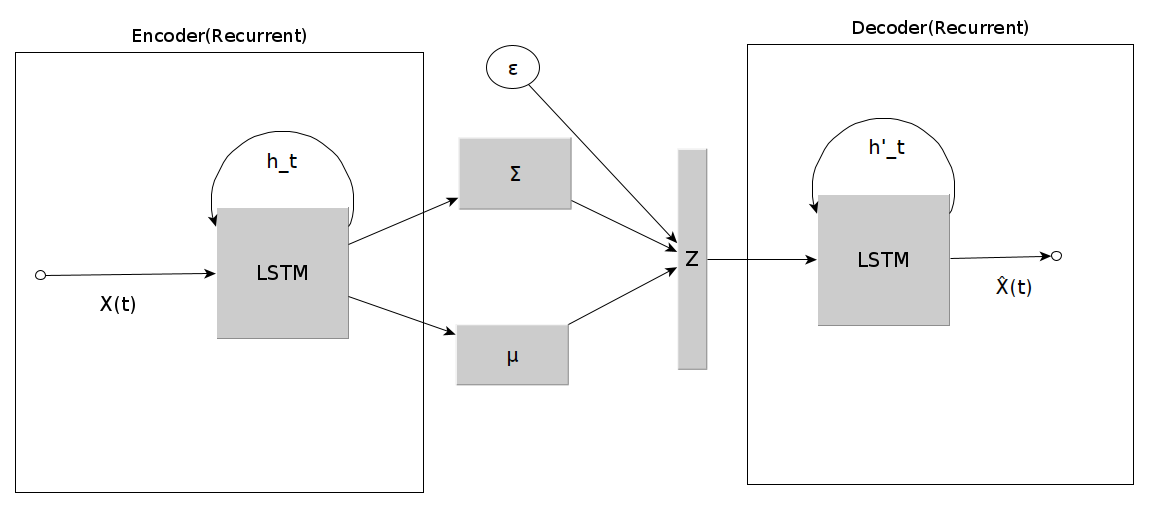
\includegraphics[scale=0.3]{architecture.png} 
%\begin{figure}
%\centering
%  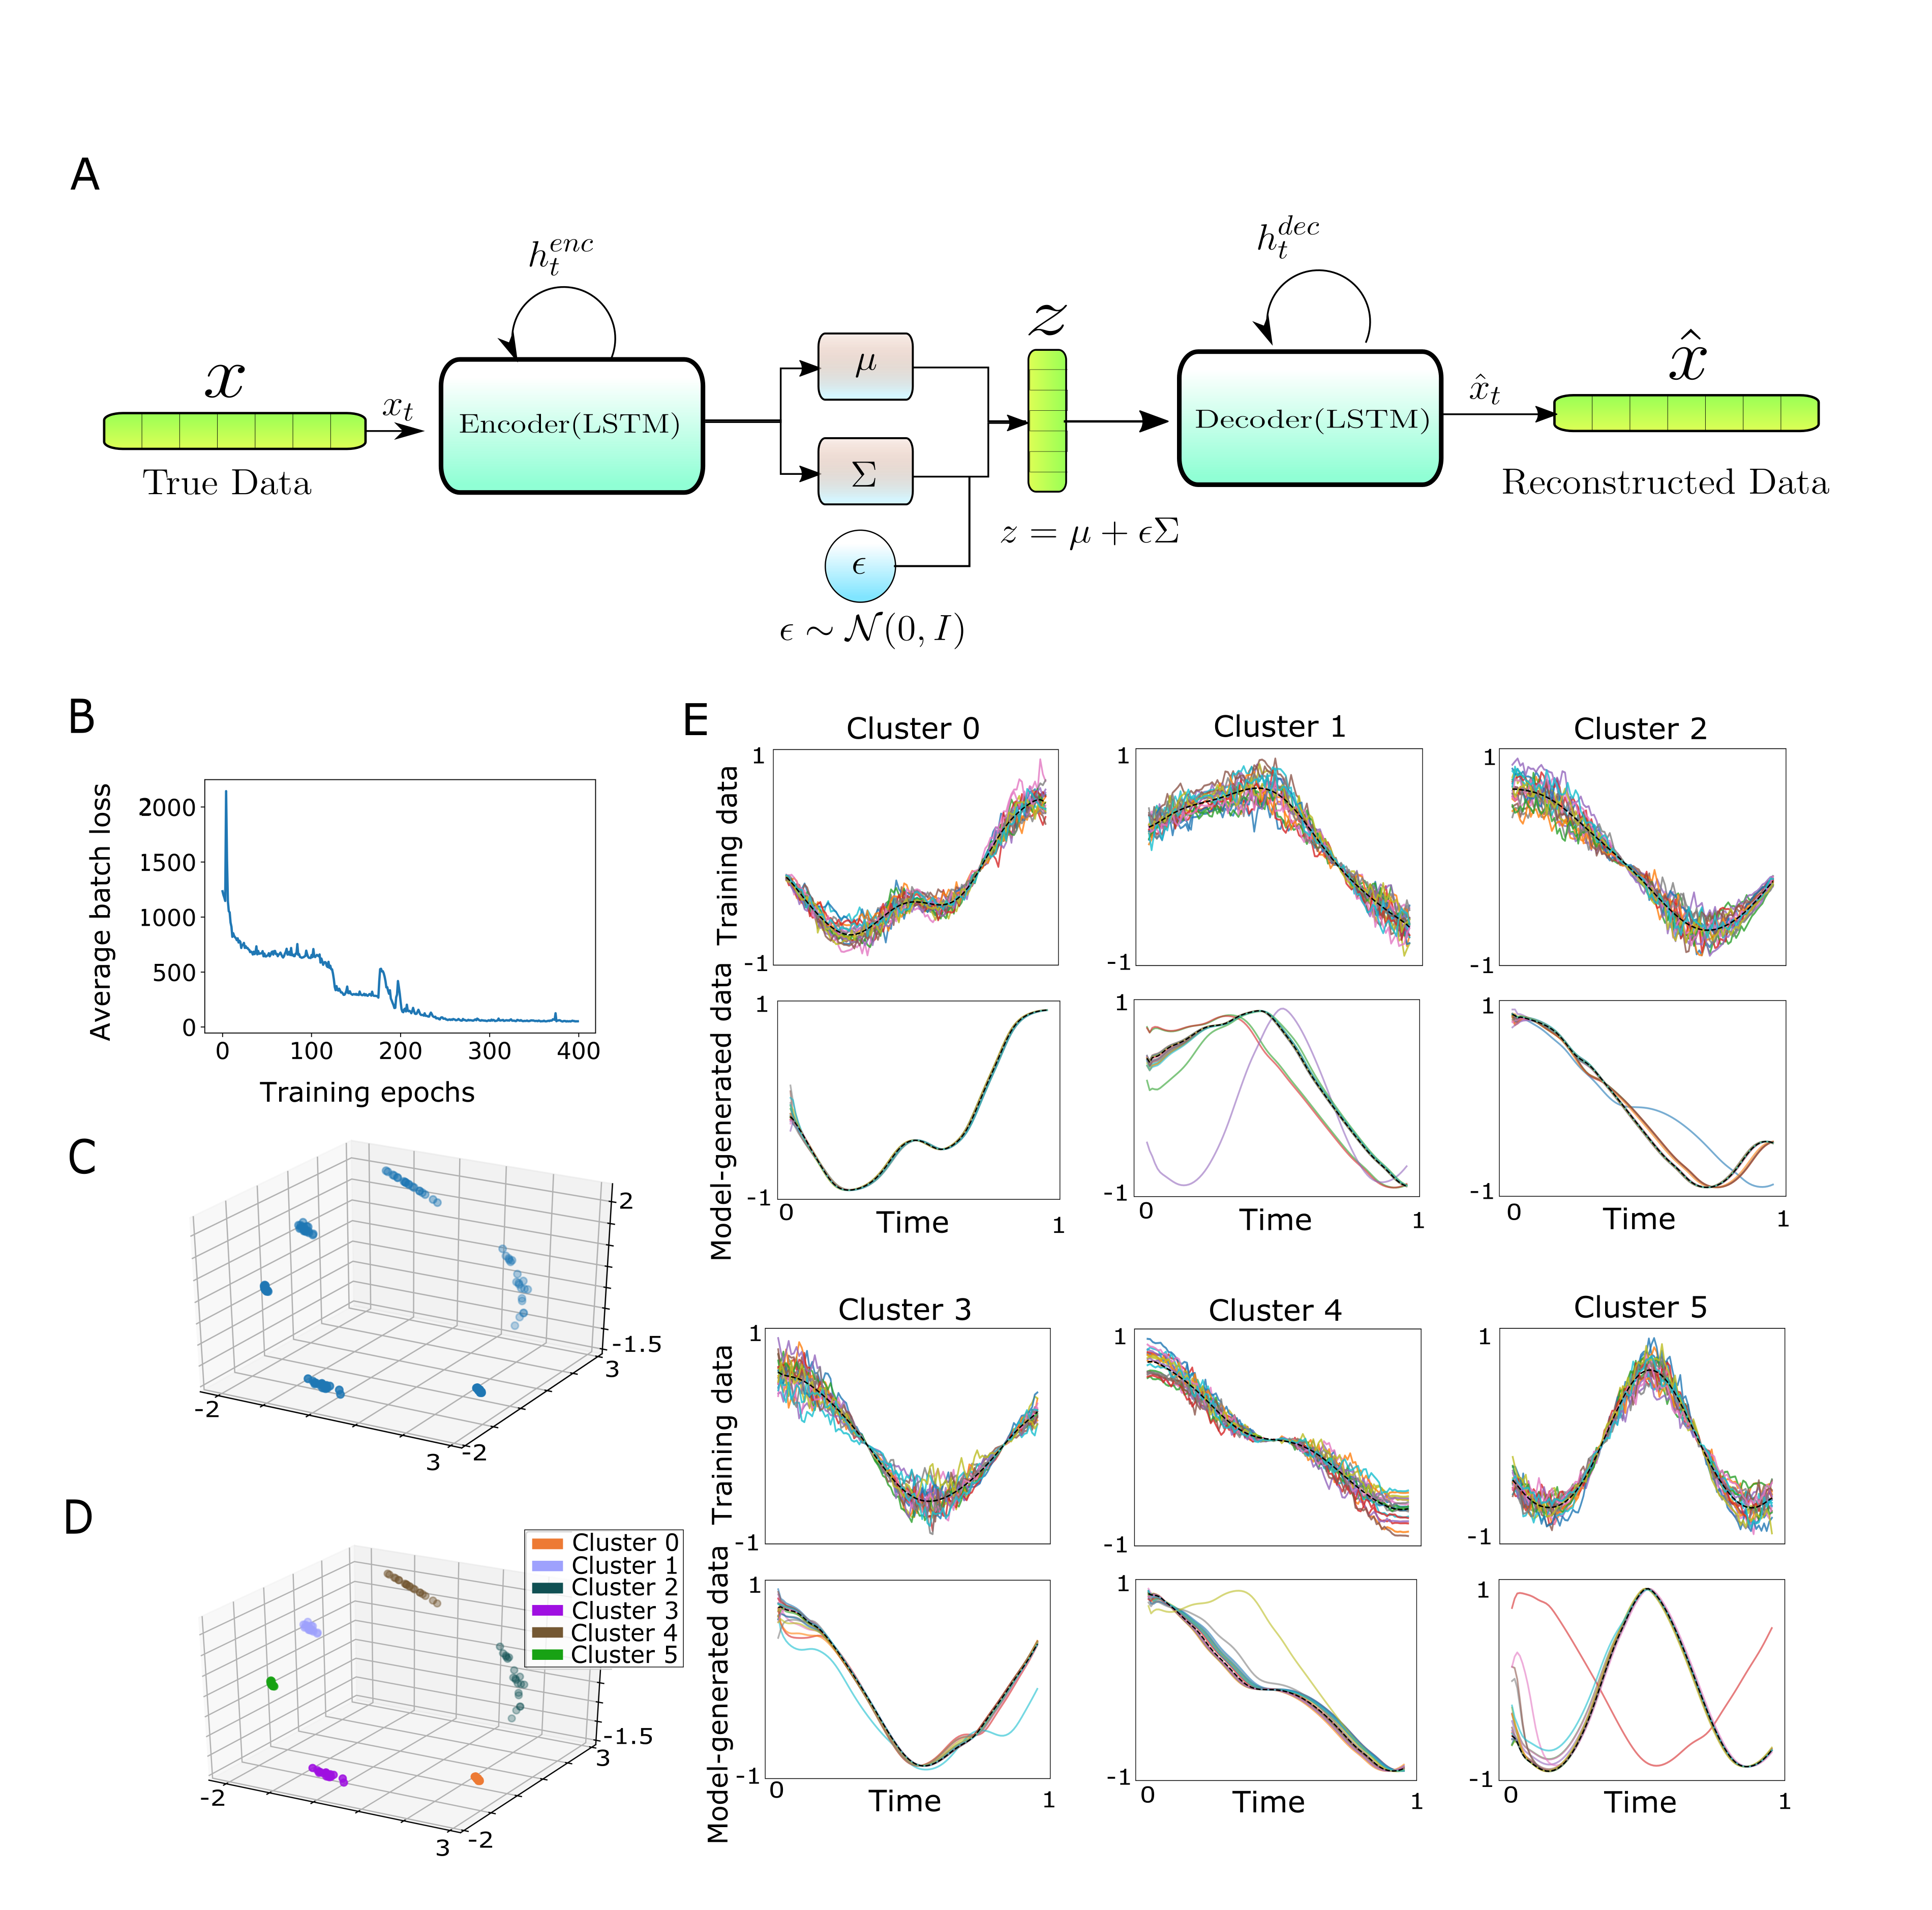
\includegraphics[width=\linewidth]{figures/fig1.png}
% % archetecture.png: 1149x508 px, 72dpi, 40.53x17.92 cm, bb=0 0 1149 508
% \caption{Schematic diagram of RVAgene.}
% \label{fig:scheme}
%\end{figure}
%\end{center}


%% Probably too much detail here, but may want to cite the refs. 
%So far, we haven't specified anything about architecture of the encoder and decoder networks of a VAE, except that they learn certain functions modelling the posterior and likelihood probabilities  of our generative story of the data we are interested in. In general we could make them a fully connected neural network. But, since we are interested in handling sequential (time-series) data, we expect a specific structure of those functions. Intuitively, the $t$-th time point of input sequenece $\vx$ should be causally dependent only on its previous timepoints (upto $t-1$).  Therefore, instead of designing a completely agnostic network (e.g. fully connected layers), we can use a recurrent architecture for the encoder and decoder, which are well established in modelling sequence data (e.g. text data (\cite{Nallapati2016}), time-series data (\cite{Malhotra2015})). This in essence reduces the search space of the model from completely agnostic to a family of recurrent functions.
%\cite{Fabius2015} used this idea and showed how Recurrent Variational Autoencoders can be useful as a unsupervised latent representation learning and generative model for music data.


\subsection{RVAgene: A recurrent variational autoencoder to model gene expression dynamics}
Following the VAE architecture, RVAgene consists of an encoder and a decoder network with a reparameterization step in between. To incorporate the knowledge that we are modeling temporal data, recurrent neural networks offer an ideal architecture to use for both the encoder and the decoder networks. Recurrent and VAE networks have been successfully combined elsewhere, e.g. for textual \citep{Nallapati2016} and time series data \citep{Malhotra2015}.
\par
The architecture of RVAgene is based on \citet{Fabius2015}. An input sequence (i.e. gene) $x \in \vx$, $x = (x_1,x_2,...,x_t,...,x_T)$ is encoded using a recurrent function described by a long short-term memory (LSTM) unit. LSTM units are the state-of-the-art in recurrent architectures, since they are robust against the vanishing gradient problem for longer sequences, unlike other recurrent units (see details in \citet{Hochreiter1997}). We encode $x$ in the following manner:
\begin{align*}
 h_{t+1}^{enc} &= \textrm{LSTM}(W_{enc}^Th_t^{enc} + W_{inp}^T{x_t}+b_{enc}), \numberthis \label{lstm}
\end{align*}
where ($W_{enc}$, $W_{inp}$ and $b_{enc}$) are network weight parameters, and the hidden states $h_t$ represent information shared over timepoints in the LSTM. The dimension of the $h_t$ (and  $W_{enc}$) is given by a hyperparameter (``hidden-size''). The encoded $h_{t+1}$ are used to parametrize the posterior mean and variance from $x$, with mean $\mu_z$ and diagonal covariance $\sigma_z$ as:
%represent this mean and diagonal covariance matrix of the normal distribution an input $x$ is getting encoded to. 

\begin{align*}
 \mu_z &= W_{\mu}^Th_{T+1}^{enc} + b_{\mu} \numberthis \label{mu}\\
  log(\sigma_z) &= W_{\sigma}^Th_{T+1}^{enc} + b_{\sigma}.  \label{sigma}
 \end{align*}
We then use the reparameterization step described in \citet{Kingma2014} to sample $z$ from the distribution:
\begin{align*}
 z = \mu_z + \epsilon\sigma_z, \numberthis 
\end{align*}
where, for known $\epsilon$, backpropagation through the sampling step is possible while training the network.
\par
For the decoder network, the first state $h_1$ is calculated from $z$, and the recurrent formulation follows by reconstructing $x$ as $\hat{x} = (\hat{x}_1,\hat{x}_2,...,\hat{x}_t,...,\hat{x}_T )$, thus:
\begin{align*}
 h_1^{dec} &= \textrm{sigm}(W_{z}^Tz + b_{z})   \\
h_{t+1}^{dec} &= \textrm{LSTM}(W_{dec}^Th_t^{dec} + W_{out}^T{\hat{x}_t}+b_{dec}) \numberthis \label{decoder_lstm} \\
\hat{x}_t &= \textrm{sigm}(W_{out}^Th_t^{dec} + b_{out}), \\
\end{align*}
where $\textrm{sigm}(u) = \frac{1}{1 + e^{-u}}$ is the sigmoid activation function, and ($W_i, b_i$) are the network weight parameters. A schematic diagram of the network is shown in \hyperref[fig:fig2]{Fig. 1A}, which can now be trained using backpropagation, to minimize the objective function: 
\begin{align*}
    \cL(\theta, x) = D_{KL}(\cN(\mathbf{\mu}_z,\Sigma_z)||\cN(\mathbf{0},\vI)) + |x - \hat{x}|, \numberthis \label{lossfunction}
\end{align*}
where $\mathbf{\mu}_z$ and $\Sigma_z = \textrm{diag}(\sigma_z)$ are calculated from $x$ by the encoder.
\par 
To evaluate the accuracy of RVAgene, we need an appropriate error measure. For each gene in the test set, we calculate the $L1$ reconstruction error between generated data $\hat{x}$ and true data $x$, averaged over all time points. We normalize the data to lie in $[0,1]$ to avoid skewing the error by differences in gene expression magnitudes. Thus we define:
\begin{align}
    \textrm{Reconstruction error}(x,\hat{x}) = \frac{1}{T}\sum_{t}| s(\hat{x})_t - s(x)_t |,  & \text{ where } s(x) = \frac{x}{\sum_{t=1}^Tx_t}.
\end{align} 

\subsection{Generating synthetic gene expression time series data}
To test RVAgene, we generate a synthetic time series dataset. Six clusters each containing 20 genes are simulated, where for each cluster $c$, the mean gene expression time series $Y_c = (y_{c1}, y_{c2}, ..., y_{ct})$ was generated using addition or convolution and rescaling of two random sinusoidal functions of the form $k_1\textrm{sin}(k_2t)$, where $k_1,k_2$ are randomly chosen positive integers. Trajectories of cluster members were then generated by sampling from the multivariate normal $\cN(Y_c,\Sigma_c)$. We model $\Sigma_c$ as the positive definite matrix $\alpha Y_cY_c^T$, where $\alpha$ is a scaling factor, we use: $\alpha = 1/|Y_c Y_c^T|$. As defined, $\Sigma_c$ will describe nonzero correlations for all pairs of time points, $(t_i,t_j)$. This is unrealistic, so we set to 0 the entries of $\Sigma_c$ for which column and row indices have a difference of more than some threshold $T$ (we used $T=50$), reflecting the fact that correlations between time points are lost over larger time windows (temporal correlations are local). Note that under this condition, $\Sigma_c$  is no longer necessarily positive definite. The multivariate Gaussian sampler \verb+numpy.random.multivariate_normal()+ implemented in \verb+numpy+ \citep{harris2020array} was used to sample from this augmented $\Sigma_c$.
{After generating a simulated dataset by this process, we also added Gaussian noise, drawn from $\cN(0,0.7)$, to the simulated dataset to produce an additional dataset exhibiting higher levels of noise.}



\section{Results}

\subsection{RVAgene can accurately and efficiently reconstruct temporal profiles from synthetic data}
We generated a dataset of 120 genes using convolutions of sinusoidal functions (see Methods) to test
the ability of RVAgene (\hyperref[fig:fig2]{fig. 6.1A}) to learn and reconstruct noisy nonlinear
temporal profiles. An RVAgene model was trained on all 120 genes from 6 clusters with a hidden size
of 70 and a 3 dimensional latent space. The model was trained for 400 epochs, after which the
average batch objective $\cL$ function indicates convergence (\hyperref[fig:fig2]{fig. 6.1B}),
producing a three-dimensional latent space representation (\hyperref[fig:fig2]{fig. 6.1C}). K-means
clustering on the latent space (k=6) identified well-separated clusters (\hyperref[fig:fig2]{fig. 6.1D}).
%Thus, RVAgene has learnt a latent space in which different temporal profiles can be readily identified and classified using simple clustering methods. 


{\centering
\begin{figure}
  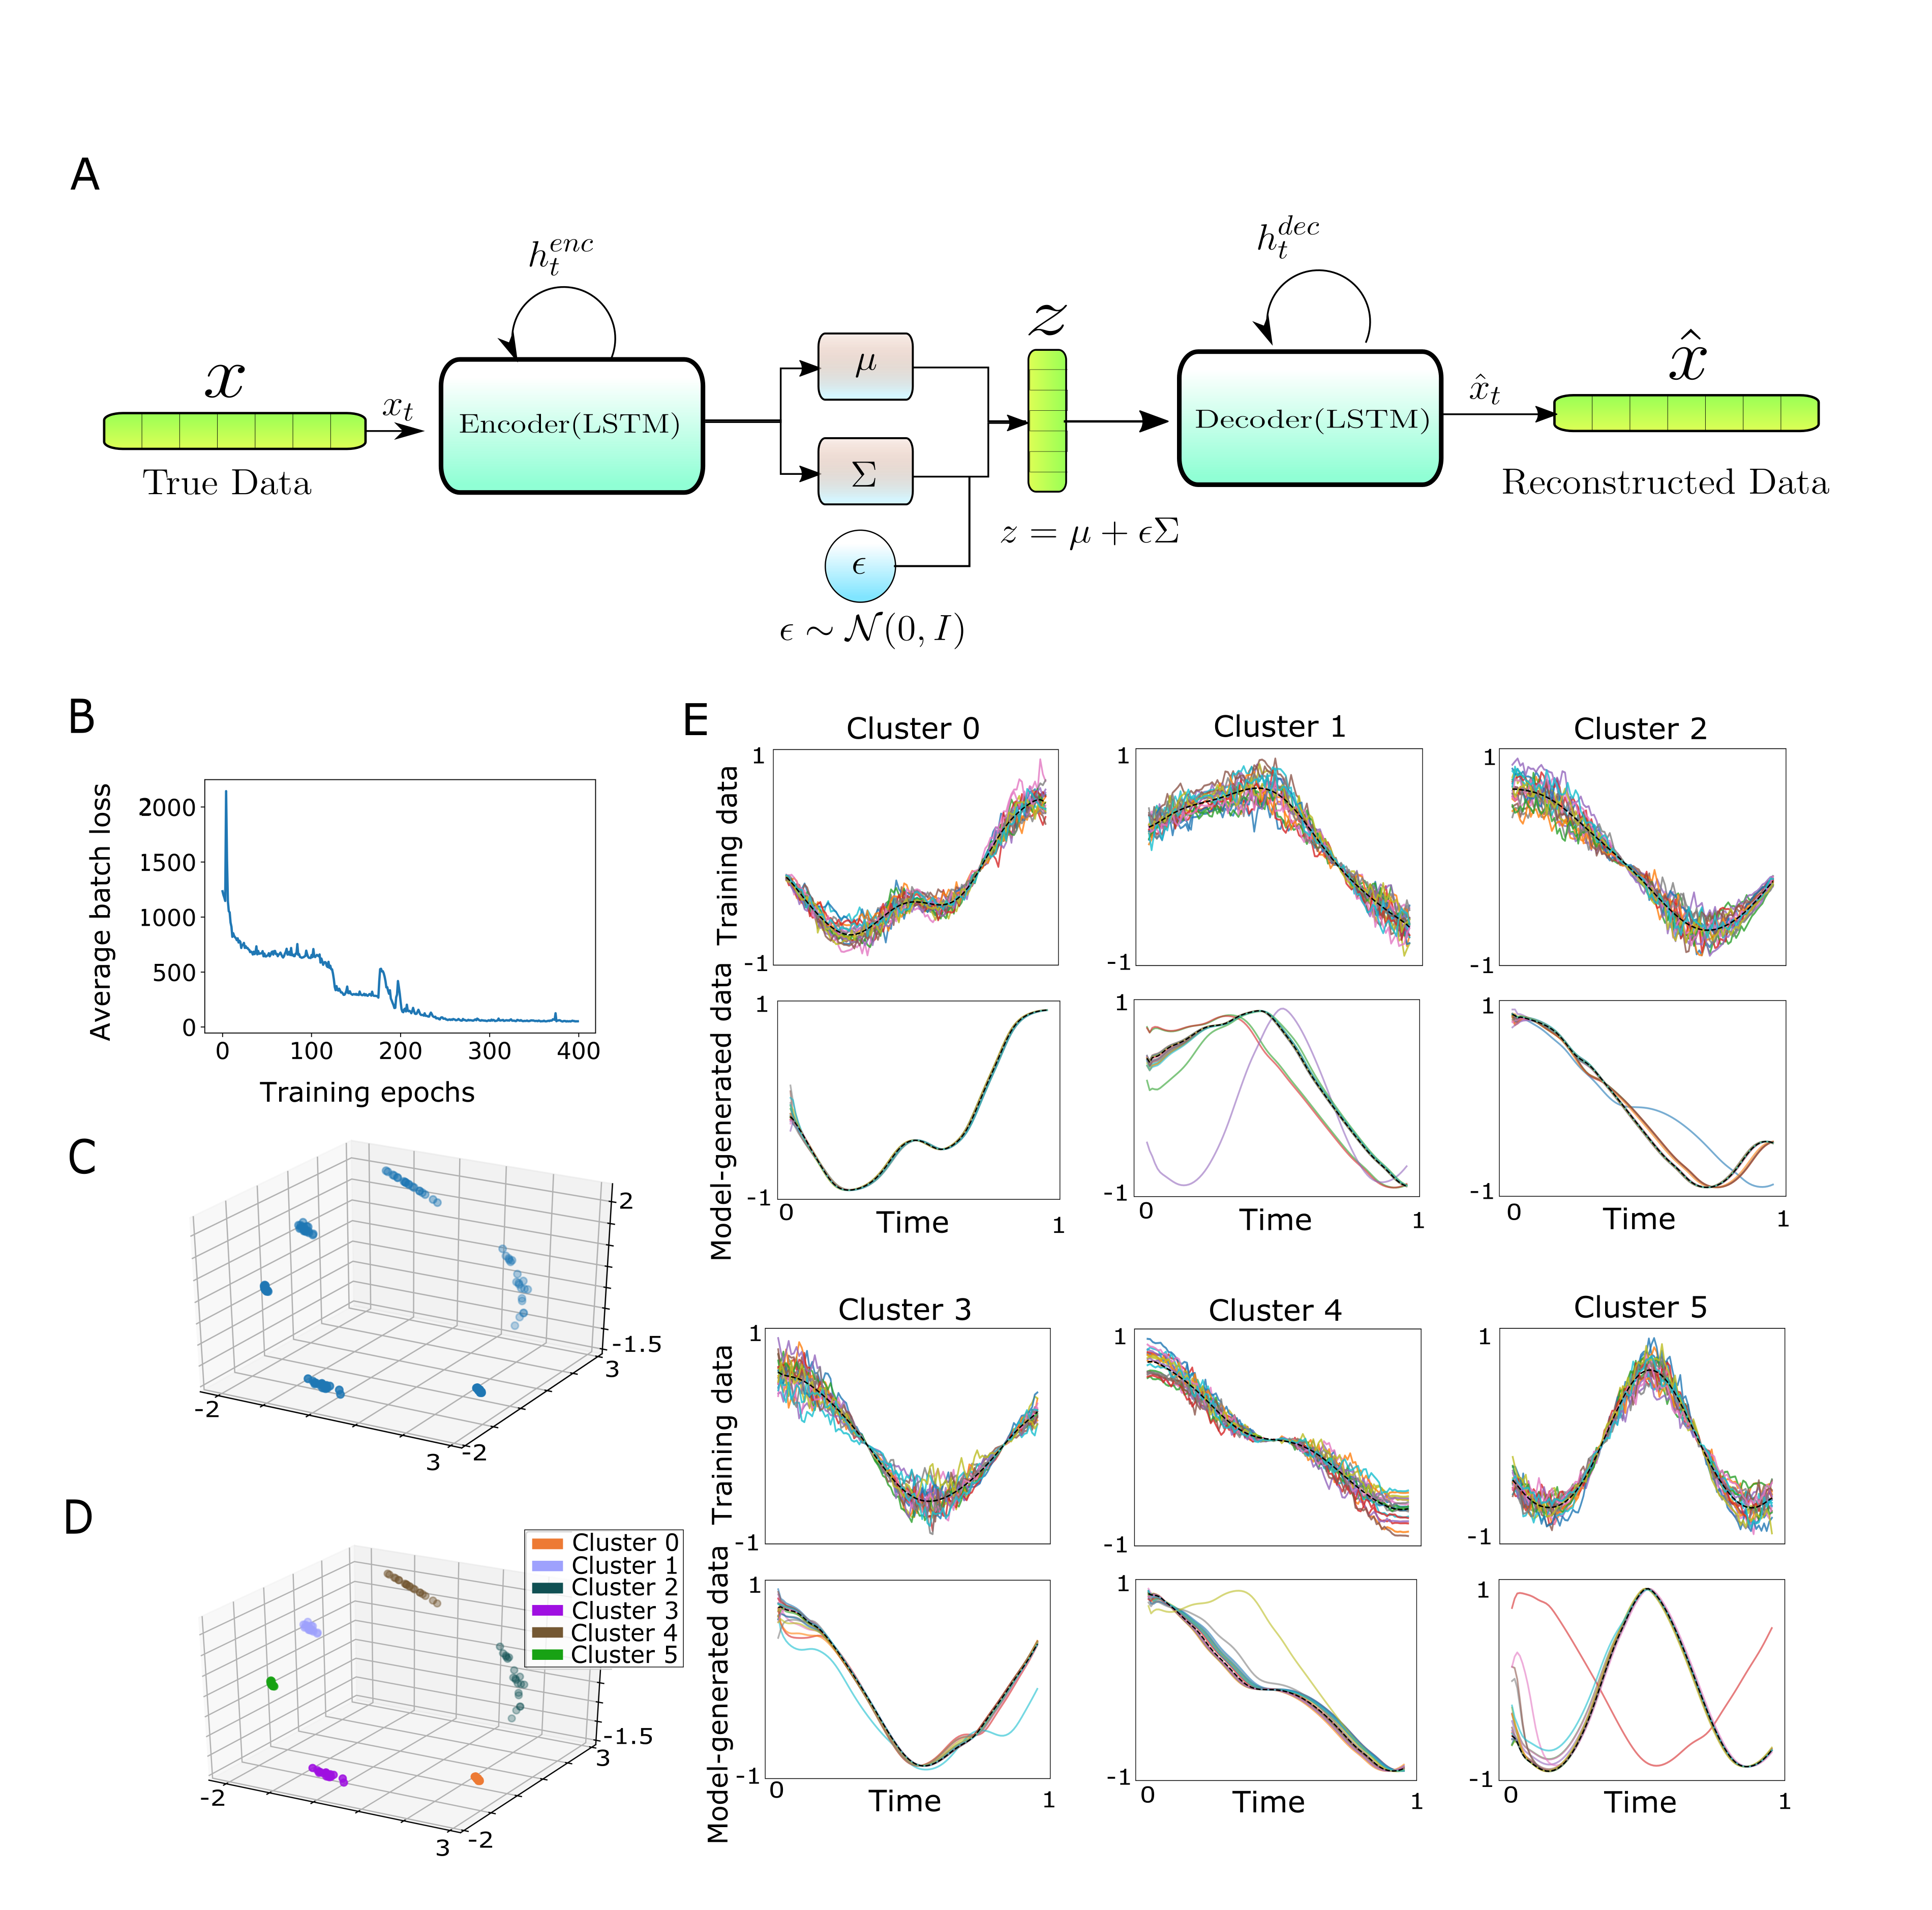
\includegraphics[width=\linewidth]{figures/fig2.png}
 % archetecture.png: 1149x508 px, 72dpi, 40.53x17.92 cm, bb=0 0 1149 508
    \caption[Unsupervised representation learning with RVAgene using synthetic data.]{\textbf{Unsupervised representation learning with RVAgene using synthetic data.} ({\bf A}) Schematic diagram of the RVAgene model. ({\bf B}) Average loss function $\cL$ as over duration of training.
    ({\bf C}) Latent space representation learnt by RVAgene model after training.
    ({\bf D}) Clusters detected by $k$-means clustering on the latent space, with $k=6$
    ({\bf E}) First and third rows show input training data used (20 simulated genes in each of six clusters); cluster means shown in black. Second and fourth rows show the model-generated data, obtained by sampling and decoding points from the latent space; decoded cluster empirical means shown in black.} 
 \label{fig:fig2}
\end{figure}
}
%%\tcr{I'm not sure about this in light of Svensson et al. we should discuss it.} 
RVAgene modeling followed by k-means clustering on the latent space identified 6 clusters with perfect fidelity between predicted and true clusters. One might reasonably ask, why use a neural network for this task? Simpler dimensionality reduction methods (e.g. PCA, t-SNE, or a non-variational autoencoder) would also find the correct solution. RVAgene has the advantage over these methods that the underlying structure of the latent space leads to interpretability. A point in reduced PCA or t-SNE space that does not overlap with a data point is not interpretable. Traditional autoencoders lack regularity in the latent space, i.e. even for a representation with arbitrary accuracy (a reconstruction error of zero), decoding a point that does not correspond to a training data point can result in nonsensical generated data, even if the decoded point is arbitrarily close to a training data point. Variational Auoencoders remedy this by learning a regularized or smoother distribution on the latent space. In this sense, the KL-divergence term in the VAE loss function can be thought of as a regularizer. This property enables RVAgene to generate new gene expression dynamics by decoding points from different regions of the latent space, having properties similar to clusters nearby to those points.


To demonstrate the generative properties of the RVAgene latent space, we sample points from
multivariate Normal distributions, centered on the empirical mean of each cluster with variance of
0.4, i.e. $\cN(\mu_c, 0.4I)$, where $\mu_c$ is the empirical mean of the cluster and $\vI$ is the
identity matrix in $\mathbb{R}^3$. Corresponding to each cluster, we sample 20 points in the latent
space, and use the decoder network to generate new time series data (\hyperref[fig:fig2]{fig. 6.1E}). Most of the points sampled generate trajectories that belong to the correct cluster. Moreover, we identify cases  corresponding to transitions between clusters. For example, some points sampled near Cluster 2 generate trajectories that are similar to members of Cluster 4, and vice versa. This makes sense due to the similarity between the temporal profiles of Clusters 2 and 4. A similar correspondence is observed between Clusters 1 and 5.
{We note that in a few cases the generated data have profiles that differ from their cluster of
origin and appear most similar to those of another cluster. This occurs when points are sampled
close to neighboring clusters, e.g. the red line for Cluster 5 in \hyperref[fig:fig2]{fig. 6.1E} has been sampled from a point close to cluster 3.}
We also observe some generated trajectories that display intermediate profiles between two or more clusters: the decoder function learnt by RVAgene is smooth, and gives rise to meaningful representations of points across regions of the latent space. 
\par
RVAgene offers additional functionality as a tool for removing noise from the data. Via sampling and
decoding points from the latent space, RVAgene reconstructs trajectories that are smooth and
de-noised relative to the input data (\hyperref[fig:fig2]{fig. 6.1E}, \hyperref[fig:figS1]{Fig. S16}). Similar neural network approaches have been proposed to denoise from single-cell data, e.g. using a deep count autoencoder \citep{eraslan2019single}. RVAgene provides data denoising as a by-product of its primary functionality: learning patterns of dynamic gene expression.
\par
{To investigate the impact of input noise levels on RVAgene performance, we added Gaussian noise
drawn from $\cN(0,0.7)$ to the simulated data to produce a dataset with higher overall noise levels.
RVAgene learns a latent space shown in (\hyperref[fig:figS1]{Fig. S16A}) from which six clusters are
identified by k-means clustering (\hyperref[fig:figS1]{Fig. S16B}). It is notable that the clusters
identified in the latent space are not as clear in this case as for lower noise levels
(\hyperref[fig:fig2]{fig. 6.1}), however RVAgene can still reconstruct the distinct profiles with high confidence. To illustrate this, we plot the original training data alongside model-generated data, sampled at random points in the latent space from  $\cN(\mu,0.4\bI)$ around each cluster mean $\mu$ for each of the 6 clusters (\hyperref[fig:figS1]{Fig. S16C}). From these simulations, RVAgene appears able to separate even relatively high levels of noise from the signal, in order to learn a smooth encoding and corresponding generative process for distinct temporal patterns.}

%Similar to other VAE-based tools for the analysis of single-cell data, RVAgene is efficient and scalable for use with large datasets. We compared the performance of RVAgene with a Bayesian nonparametric approach for the analysis of gene expression time series data (Dirichlet Process Gaussian Process \citep{McDowell2018}. Using either CPU or GPU computing, the time and memory gains are substantial, enabling the analysis of larger datasets than would otherwise be possible (\hyperref[supp]{Fig. S1}). Analysis of RVAgene using simulated temporal data highlights the ability of such an architecture as means to study and generate gene expression dynamics. It enables learning of an unsupervised representation space, on which post-processing (e.g. unsupervised clustering) can be performed, as well as data denoising, and the generation of new time series data from arbitrary points in the latent space.
\par
It is inevitably challenging to include sufficient dimensionality and variation in synthetic datasets to accurately capture biological processes such as those we observe in experimental datasets. Thus, in the subsequent two sections, we test the capabilities of RVAgene on two whole-genome biological datasets: embryonic stem cell differentiation, and kidney injury response. As we will see, in these cases it may not be possible to characterize the latent space by simple (e.g. k-means) clustering; we need to use other means to gain insight into the features of the latent space.



\subsection{RVAgene modeling of pseudotemporally ordered data during embryonic stem cell differentiation}

We applied RVAgene to model gene expression dynamics during embryonic stem cell (ESC)
differentiation. \citet{Klein2015} identified 732 differentially expressed genes over the time
course of mouse ESC differentiation following leukemia inhibitory factor (LIF) withdrawal. Data is
gathered at four time points: 0, 2, 4, and 7 days after LIF withdrawal. (Table S2 in
\citet{Klein2015}). We ordered the data (2717 single cells) using diffusion pseudotime (DPT), which
provides robust methods for the reconstruction of single-cell temporal processes
\citep{haghverdi2016diffusion}. The root cell was randomly sampled from the initial time point
(\hyperref[fig:fig3]{fig. 6.2A}). The inferred pseudotime is highly correlated with the experimental
time points, giving confidence that true biological processes are represented over the DPT
pseudotime. The gene expression dynamics over pseudotime show considerable variability among cells.
To smooth the data, we apply a moving window average, over windows of length 40, to give 68 time
points after smoothing (\hyperref[fig:fig3]{fig. 6.2A}). 
We fit linear regression models to the smoothed pseudotime profiles of each gene
(\hyperref[fig:figS2]{Fig. S17}), and see that for the majority of genes the correlation coefficients are
$> 0.5$ (\hyperref[fig:fig3]{fig. 6.2B}), with a clear distinction between the up- and down-regulated genes over pseudotime.
\par 
An RVAgene model was trained on the data with a two-dimensional latent space, on which genes are
classified based on their correlation coefficients  (\hyperref[fig:fig3]{fig. 6.2C}). Two distinctive characteristics emerge: a) the two groups (up- and down-regulated genes) are well-separated in the latent space, and b) the two groups merge and overlap at some point, illustrating the continuity of the latent space, as discussed above. 
We compared the results of RVAgene with DPGP, an unsupervised approach for gene expression time series clustering \citep{McDowell2018}. DPGP is a hierarchical Bayesian model that estimates the number of clusters along with the cluster membership.

To assess the correspondence between methods, genes clustered by DPGP (\hyperref[fig:figS3]{Fig. S18})
were projected onto the RVAgene latent space (\hyperref[fig:fig3]{fig. 6.2D}). Of the 12 clusters
detected by DPGP, the four largest can be characterized by their up- and down-regulation profiles
over pseudotime. On the RVAgene latent space, we find that genes sampled from each of the DPGP
clusters appear close together, and moreover, are represented on a spectrum from upregulation to
downregulation (\hyperref[fig:fig3]{fig. 6.2D}). The goals of RVAgene and DPGP are to some degree complementary: DPGP characterizes gene expression profiles discretely with no need for prior information, while RVAgene characterizes profiles with a continuous representation, that can explain smooth changes in patterns.

%DPGP is a hierarchical Bayesian model that estimates the number of clusters along with the cluster membership, and outputs a posterior mean function and covariance matrix for each gene cluster. In contrast to RVAgene, DPGP does not assume any structure in gene expression data, performing an agnostic search, resulting in higher resource consumption (see \hyperref[supp]{Fig. S1}). DPGP does perform unsupervised clustering, a key advantage, although it does not provide inter-cluster information or predictions, which are provided by RVAgene.


{\centering
\begin{figure}%\begin{wrapfigure}[19]{r}{75mm}
  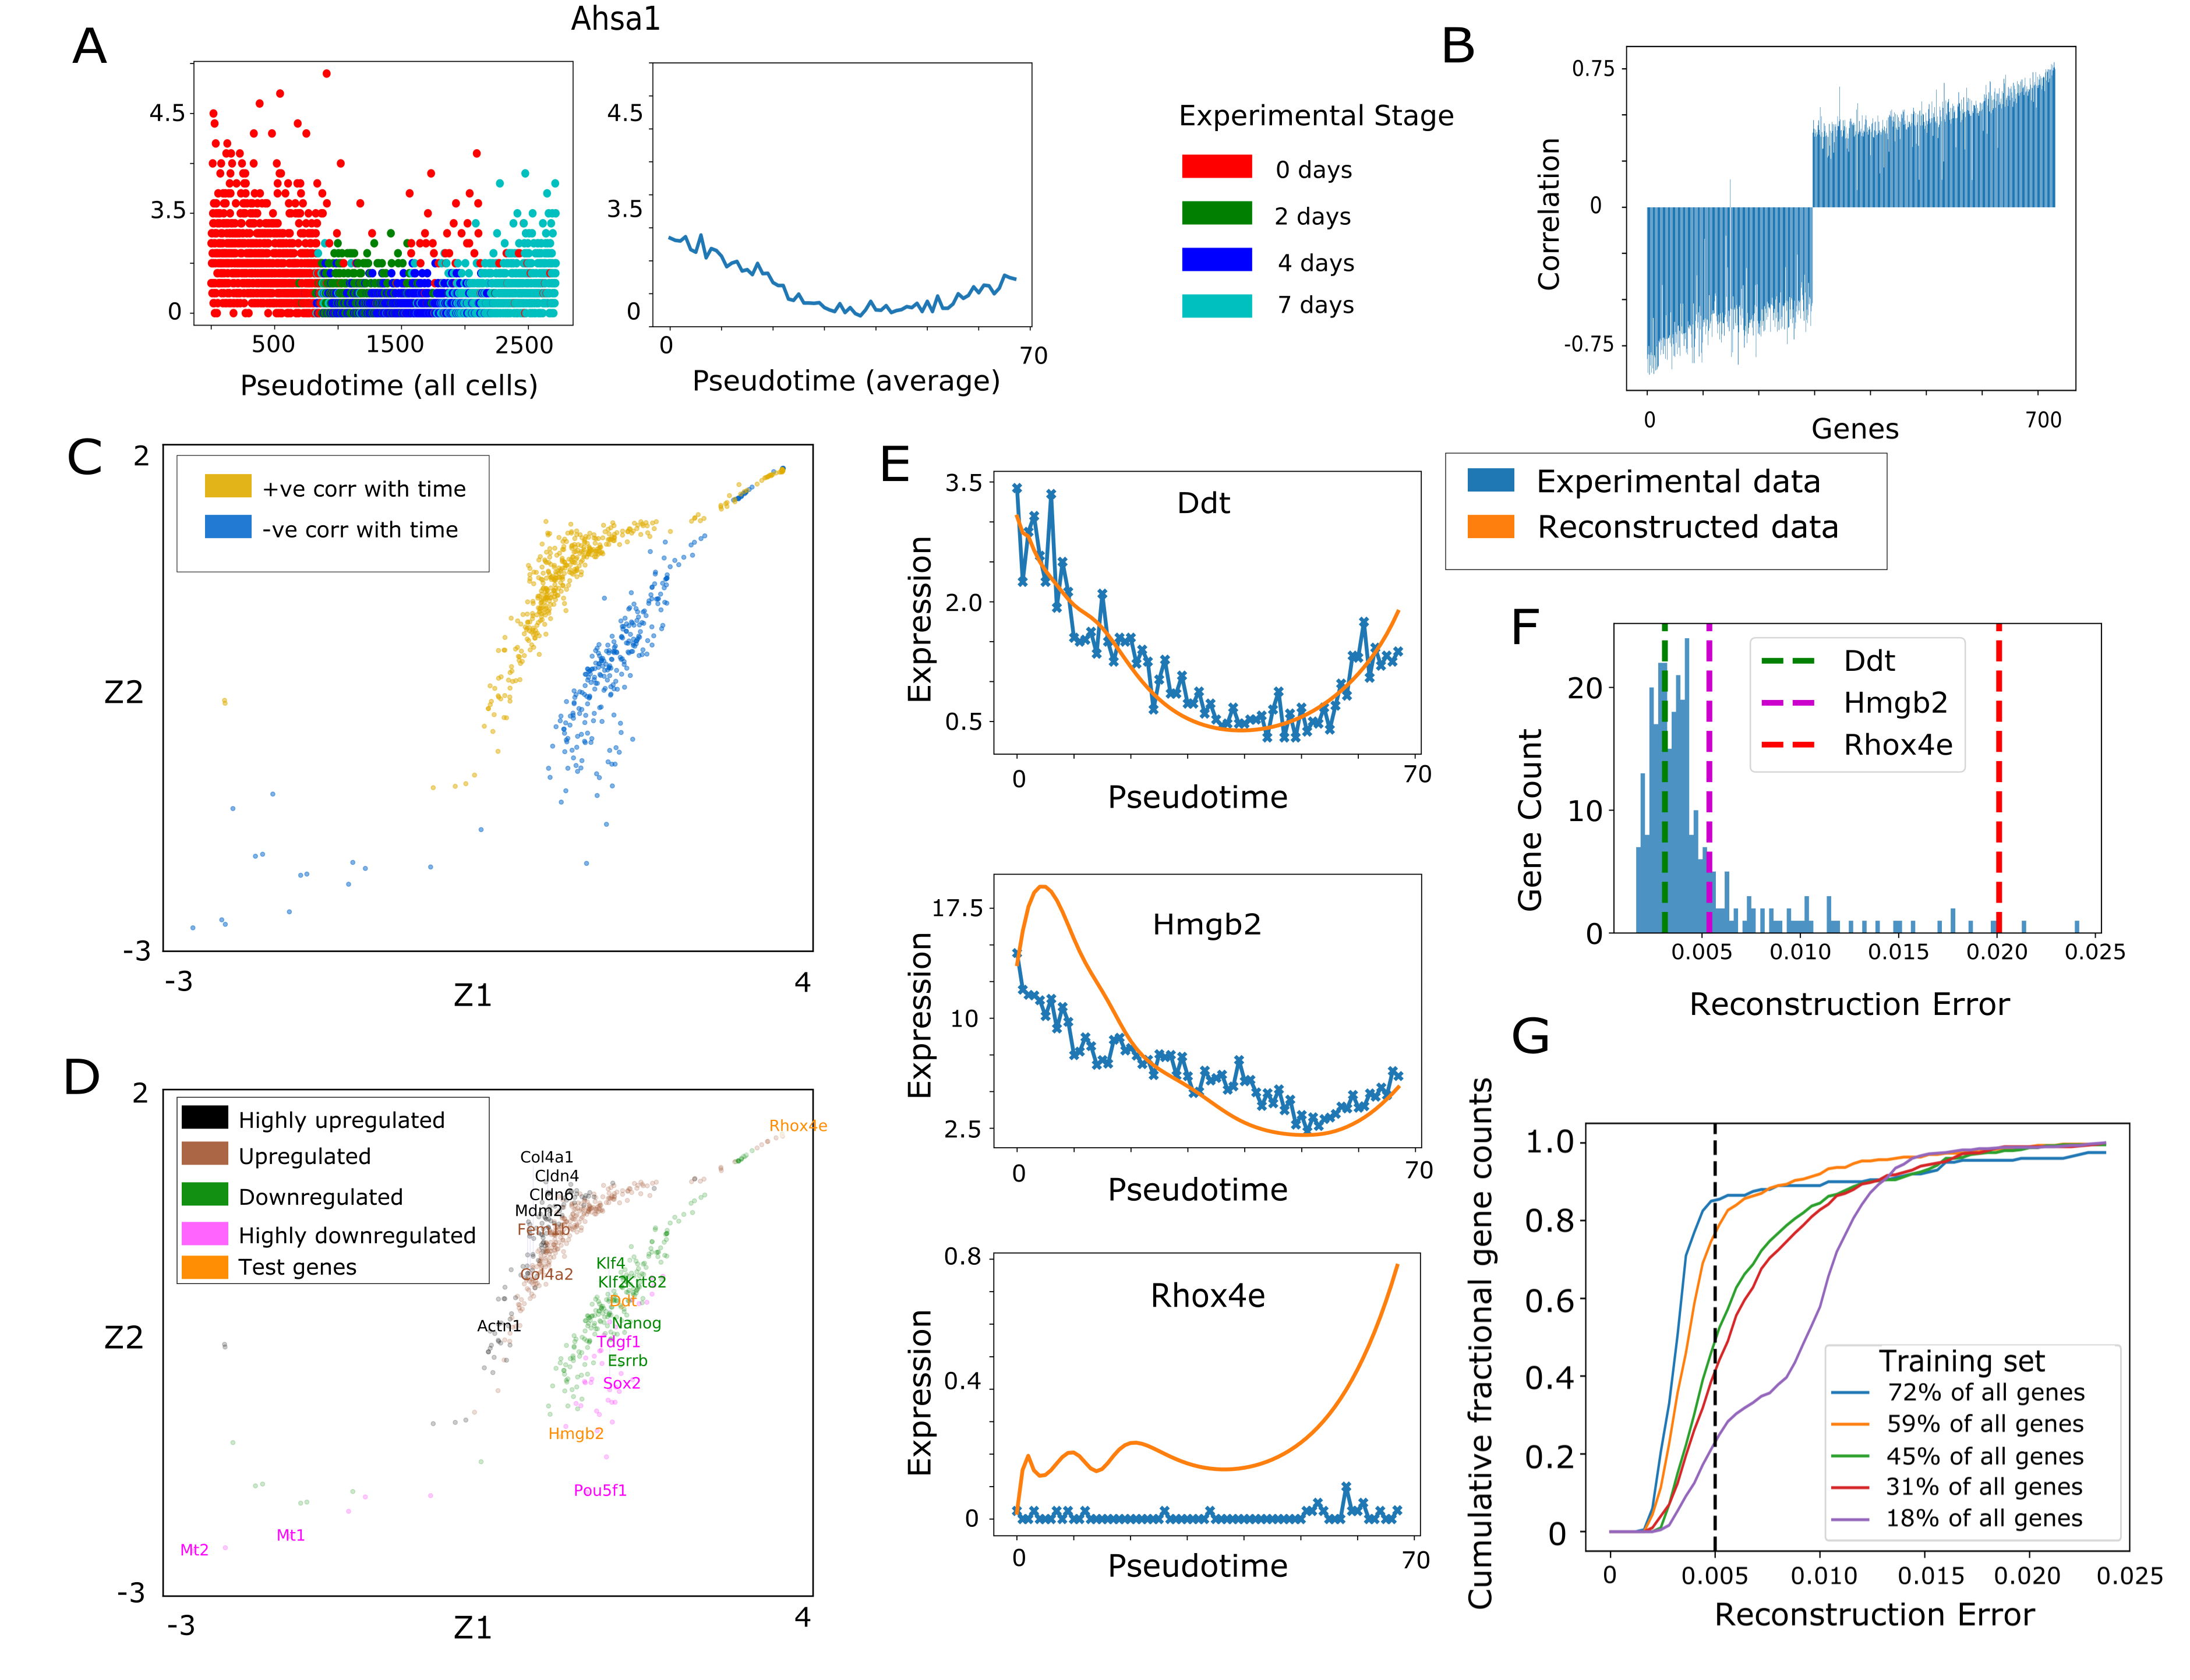
\includegraphics[width=\linewidth]{figures/esc_results.png}
 % archetecture.png: 1149x508 px, 72dpi, 40.53x17.92 cm, bb=0 0 1149 508
    \caption[Accurate reconstruction of embryonic stem cell differentiation dynamics with RVAgene.]{\textbf{Accurate reconstruction of embryonic stem cell differentiation dynamics with RVAgene.}
     ({\bf A}) Pseudotemporal ordering of 2717 single cells (data from \citep{Klein2015}), calculated using DPT; example gene shown: Ahsa1. Gene expression values given as log2(counts+1) for all cells (left), and for sliding window average (right).  ({\bf B}) Pearson correlation coefficient between gene expression and time for 732 differentially expressed genes.
    ({\bf C}) The 2D latent space learnt by an RVAgene model trained on 732 gene profiles over pseudotime, showing clear separation between upregulated and downregulated genes. ({\bf D}) Comparison of RVAgene and DPGP. The four largest clusters from DPGP are plotted on the RVAgene latent space: temporal expression patterns (from highly upregulated to highly downregulated) are in close agreement between methods. ({\bf E}) Comparison of experimental data and reconstructions. Model-generated reconstructions of three genes from the test set not used in training: Ddt, Hmgb2, and Rhox4e. Expression values are log2(counts+1).
    ({\bf F}) Distribution of average $L1$ reconstruction errors for the 300 genes used in the test set. Genes plotted in C are marked.
    ({\bf G}) Cumulative distributions of reconstruction errors on randomly sampled sets of test genes, where the full data were split into test groups of: 200 genes (train on 72\%), 300 genes (train on 59\%), 400 genes (train on 45\%), 500 genes (train on 31\%), and 600 genes (train on 18\%).}
    \label{fig:fig3}
\end{figure}
}

{\centering
\begin{figure}
  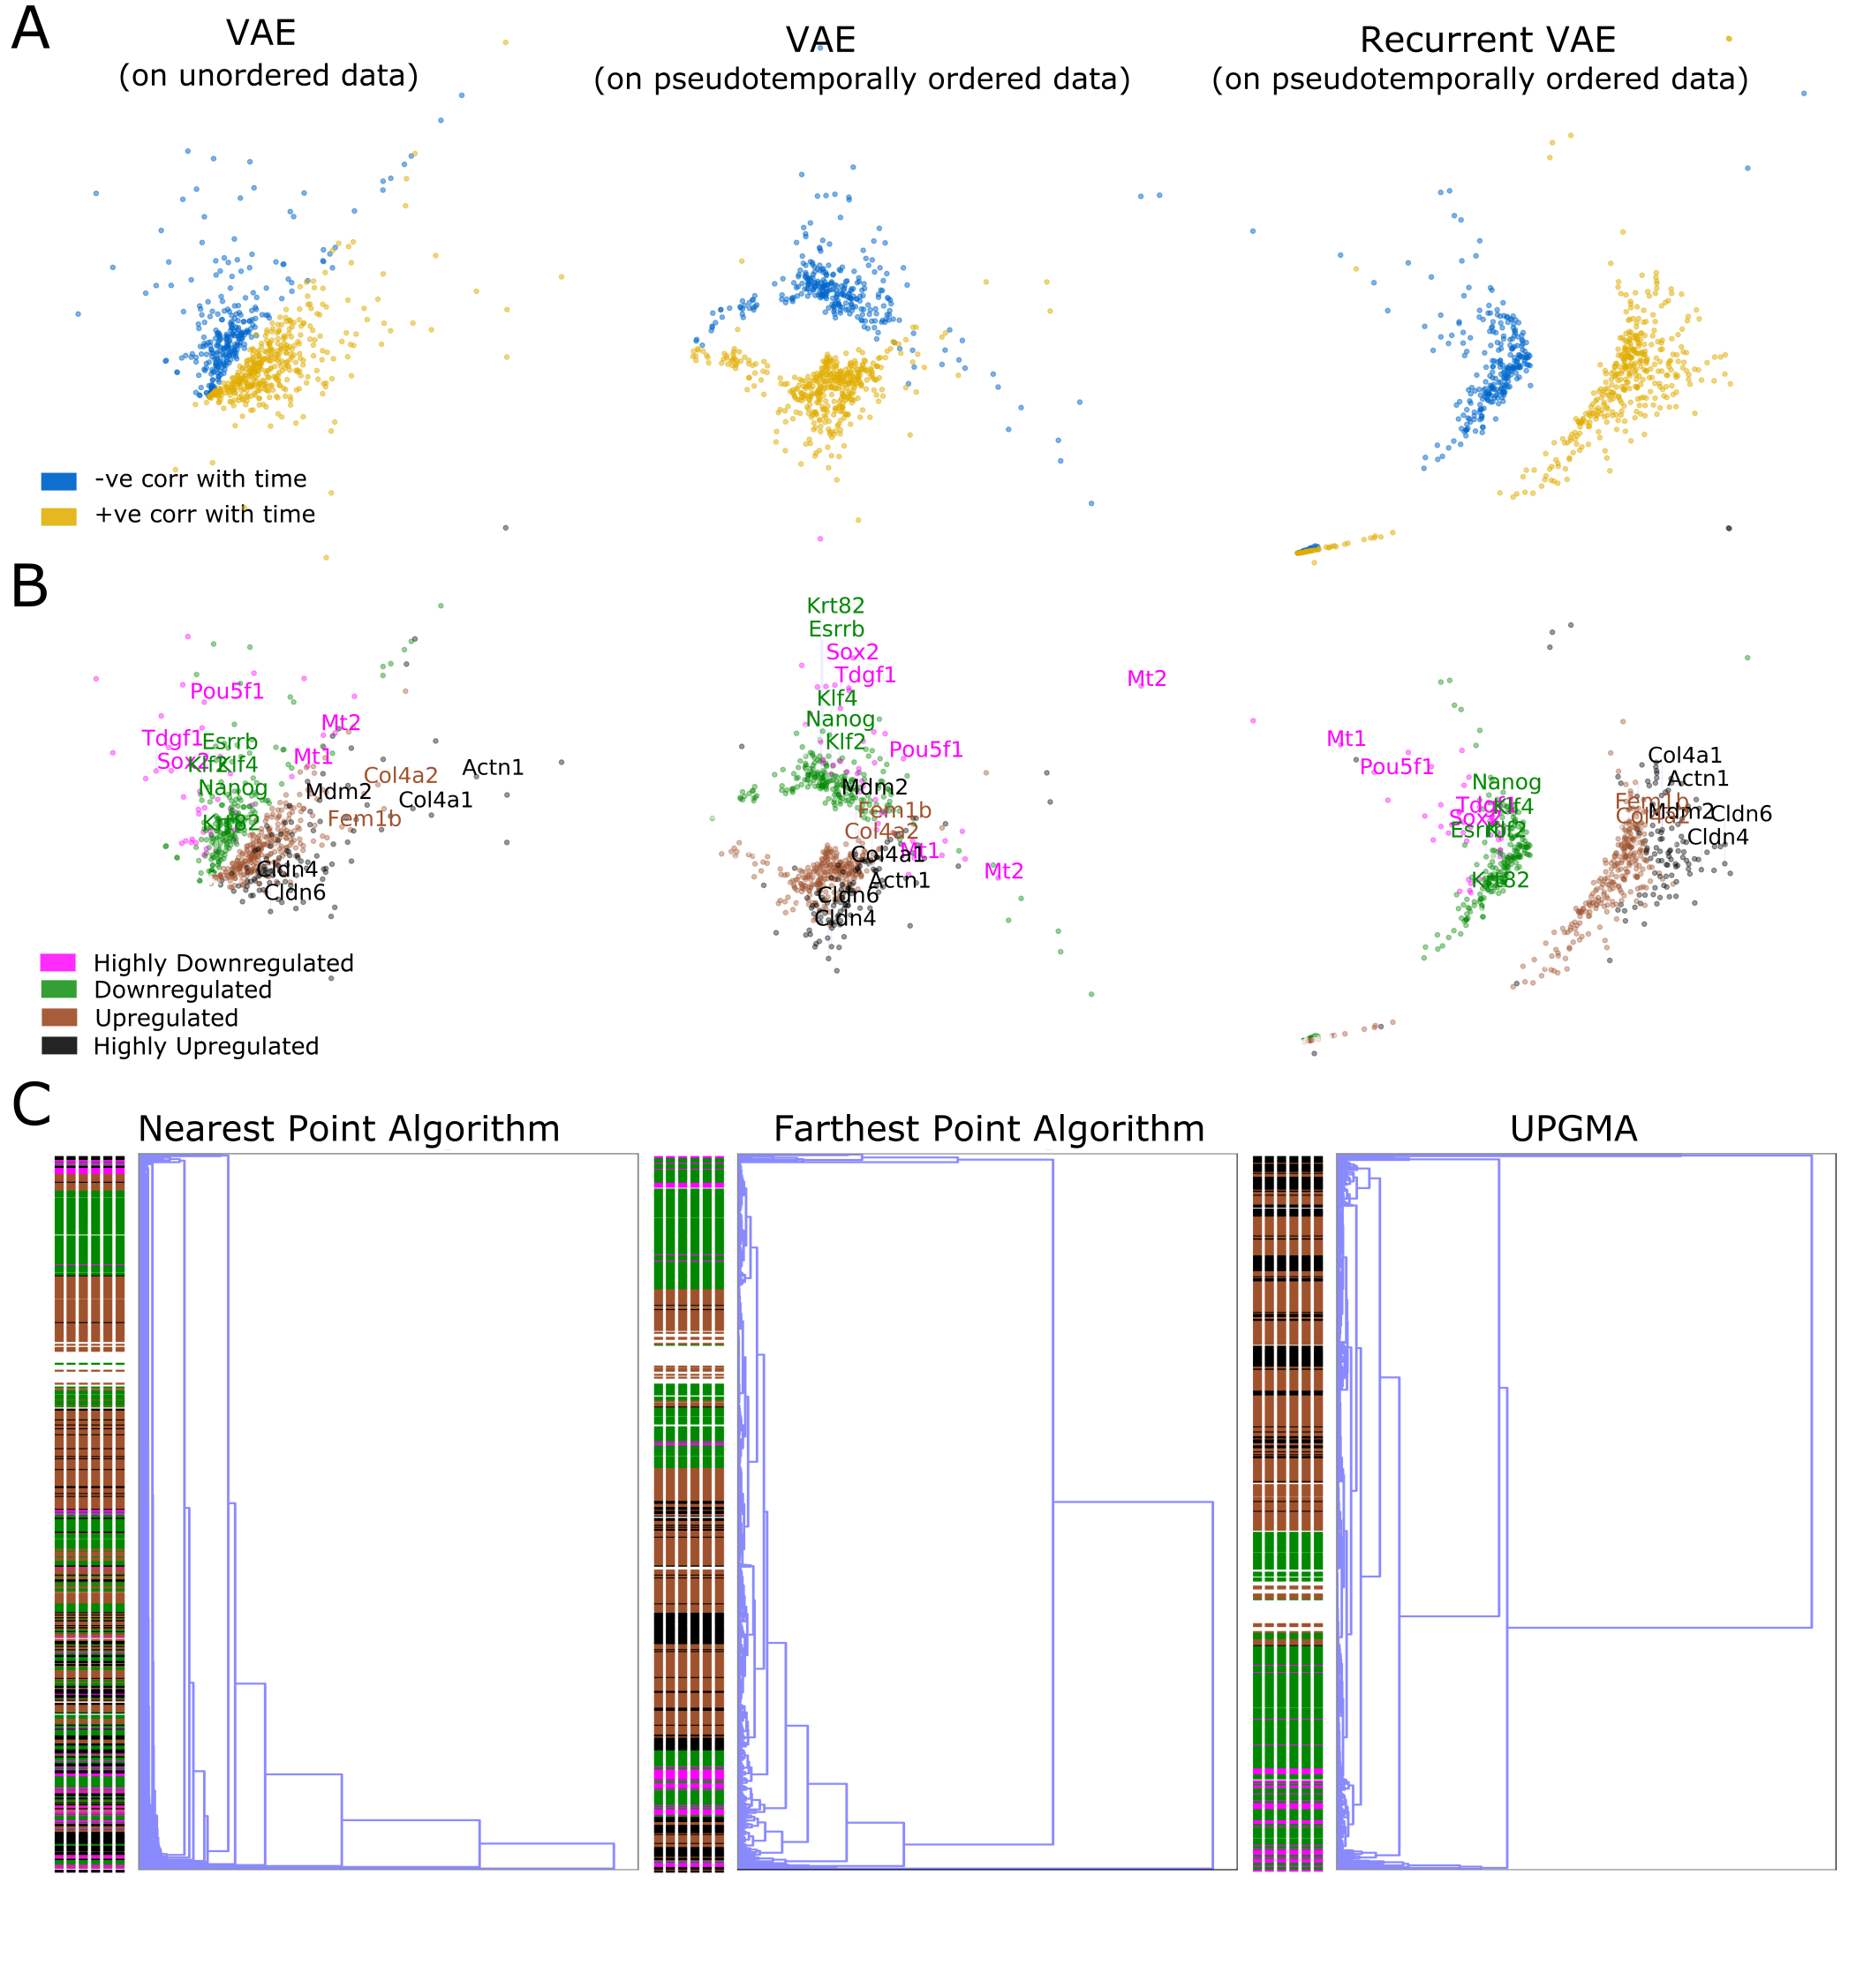
\includegraphics[width=\linewidth]{figures/vae_comp.png}
 % archetecture.png: 1149x508 px, 72dpi, 40.53x17.92 cm, bb=0 0 1149 508
    \caption[Comparison of information captured in RVAgene latent space compared to a standard fully connected VAE and results of standard hierarchical clusterings.]{\textbf{Comparison of information captured in RVAgene latent space compared to a standard fully connected VAE and results of standard hierarchical clusterings.}
    ({\bf A}) Here we show latent spaces learned by fully connected VAE and RVAgene. The pseudotemporally ordered data was also smoothed. ({\bf B}) We annotate the learned latent spaces using the top 4 clusters detected by DPGP on this dataset. In all three of these cases we report best results after relevant hyperparameter search and optimal training. ({\bf C}) We perform standard hierarchical clusterings (Nearest Point Algorithm, Farthest Point Algorithm and UPGMA (Unweighted Pair Group Method with Arithmetic mean) ) on pseudotemporally ordered and smoothed ESC data and annotate the learned representation in the same manner as in (B).} 
  \label{fig:fig4}
\end{figure}}

{
To assess the ability of the model to reconstruct genes not used during training, we kept aside 300 genes for testing and trained RVAgene on the remaining 432 genes.
We note that in this case (and in the case of single-cell datasets in general), the generative model of RVAgene produces pseudotime-smoothed gene expression trajectories, rather than being generative of raw pseudotemporal data, which tend to display overall high noise levels.
}
Reconstructed test gene expression profiles are shown for three reconstructed genes
(\hyperref[fig:fig3]{fig. 6.2E}), chosen to sample across the spectrum of reconstruction errors
(\hyperref[fig:fig3]{fig. 6.2F}). The reconstruction for {\em Ddt}, which has a reconstruction error
near the mode (\hyperref[fig:fig3]{fig. 6.2F}), shows very high accuracy. The reconstruction for
{\em Hmgb2}, which has twice the reconstruction error, still broadly captures the temporal profile
but with lesser accuracy. Finally we show the reconstruction for {\em Rhox4e}, a gene that was
sampled from the long tail of the reconstruction error distribution, i.e. does not well match the
data. Comparing these three examples with the full distribution of reconstruction errors
(\hyperref[fig:fig3]{fig. 6.2F}), we see that the large majority of genes lie to the left of {\em
Hmgb2}, i.e. have better-than-moderate accuracy. The reconstruction error of {\em Hmgb2} is close to
0.005, which we use as a cut off for ``well-reconstructed'' genes, based on analysis of individual
gene reconstructions. The cumulative reconstruction error distribution reiterates this point: 230
out of 300 genes (77\%) have a reconstruction error $\leq 0.005$ (\hyperref[fig:fig3]{fig. 6.2G}); we can conclude that the majority of test genes were faithfully reconstructed by the model.
\par
RVAgene accurately reconstructed most gene profiles using only $\sim60 {\%}$ of the data for
training (\hyperref[fig:fig3]{fig. 6.2G}), likely due to co-regulation of gene expression programs.
This led to a question: what is the smallest training gene set that can be used to accurately
reconstruct gene dynamics? We subset the data randomly into train/test sets and trained separate
RVAgene models on each. We found that reconstruction errors slowly increase as the size of the
training set decreases, but not until the training set was as low as $18\%$ of the data did the
reconstruction errors significantly increase (\hyperref[fig:fig3]{fig. 6.2G}, \hyperref[fig:figS4]{Fig. S19}). Analysis of the cumulative distribution of reconstruction errors across all groups found that RVAgene reconstructs the majority of gene temporal profiles well (defined as below a reconstruction error of 0.005) if $\geq 45\%$ of the data is used for training. The successful reconstruction of gene expression dynamics de novo while training on  small subsets of the data suggests widespread co-regulation of gene expression programs during embryonic stem cell differentiation, as found in previous work \citep{jang2017dynamics}.
% This information is a useful indicator to whether an algorithm estimating number of clusters is overfitting or underfitting (i.e. detecting too many or too few clusters), we talk about this in more detail later in \hyperref[discussion1]{Discussion} section. 

%{\centering
%\begin{figure}
%  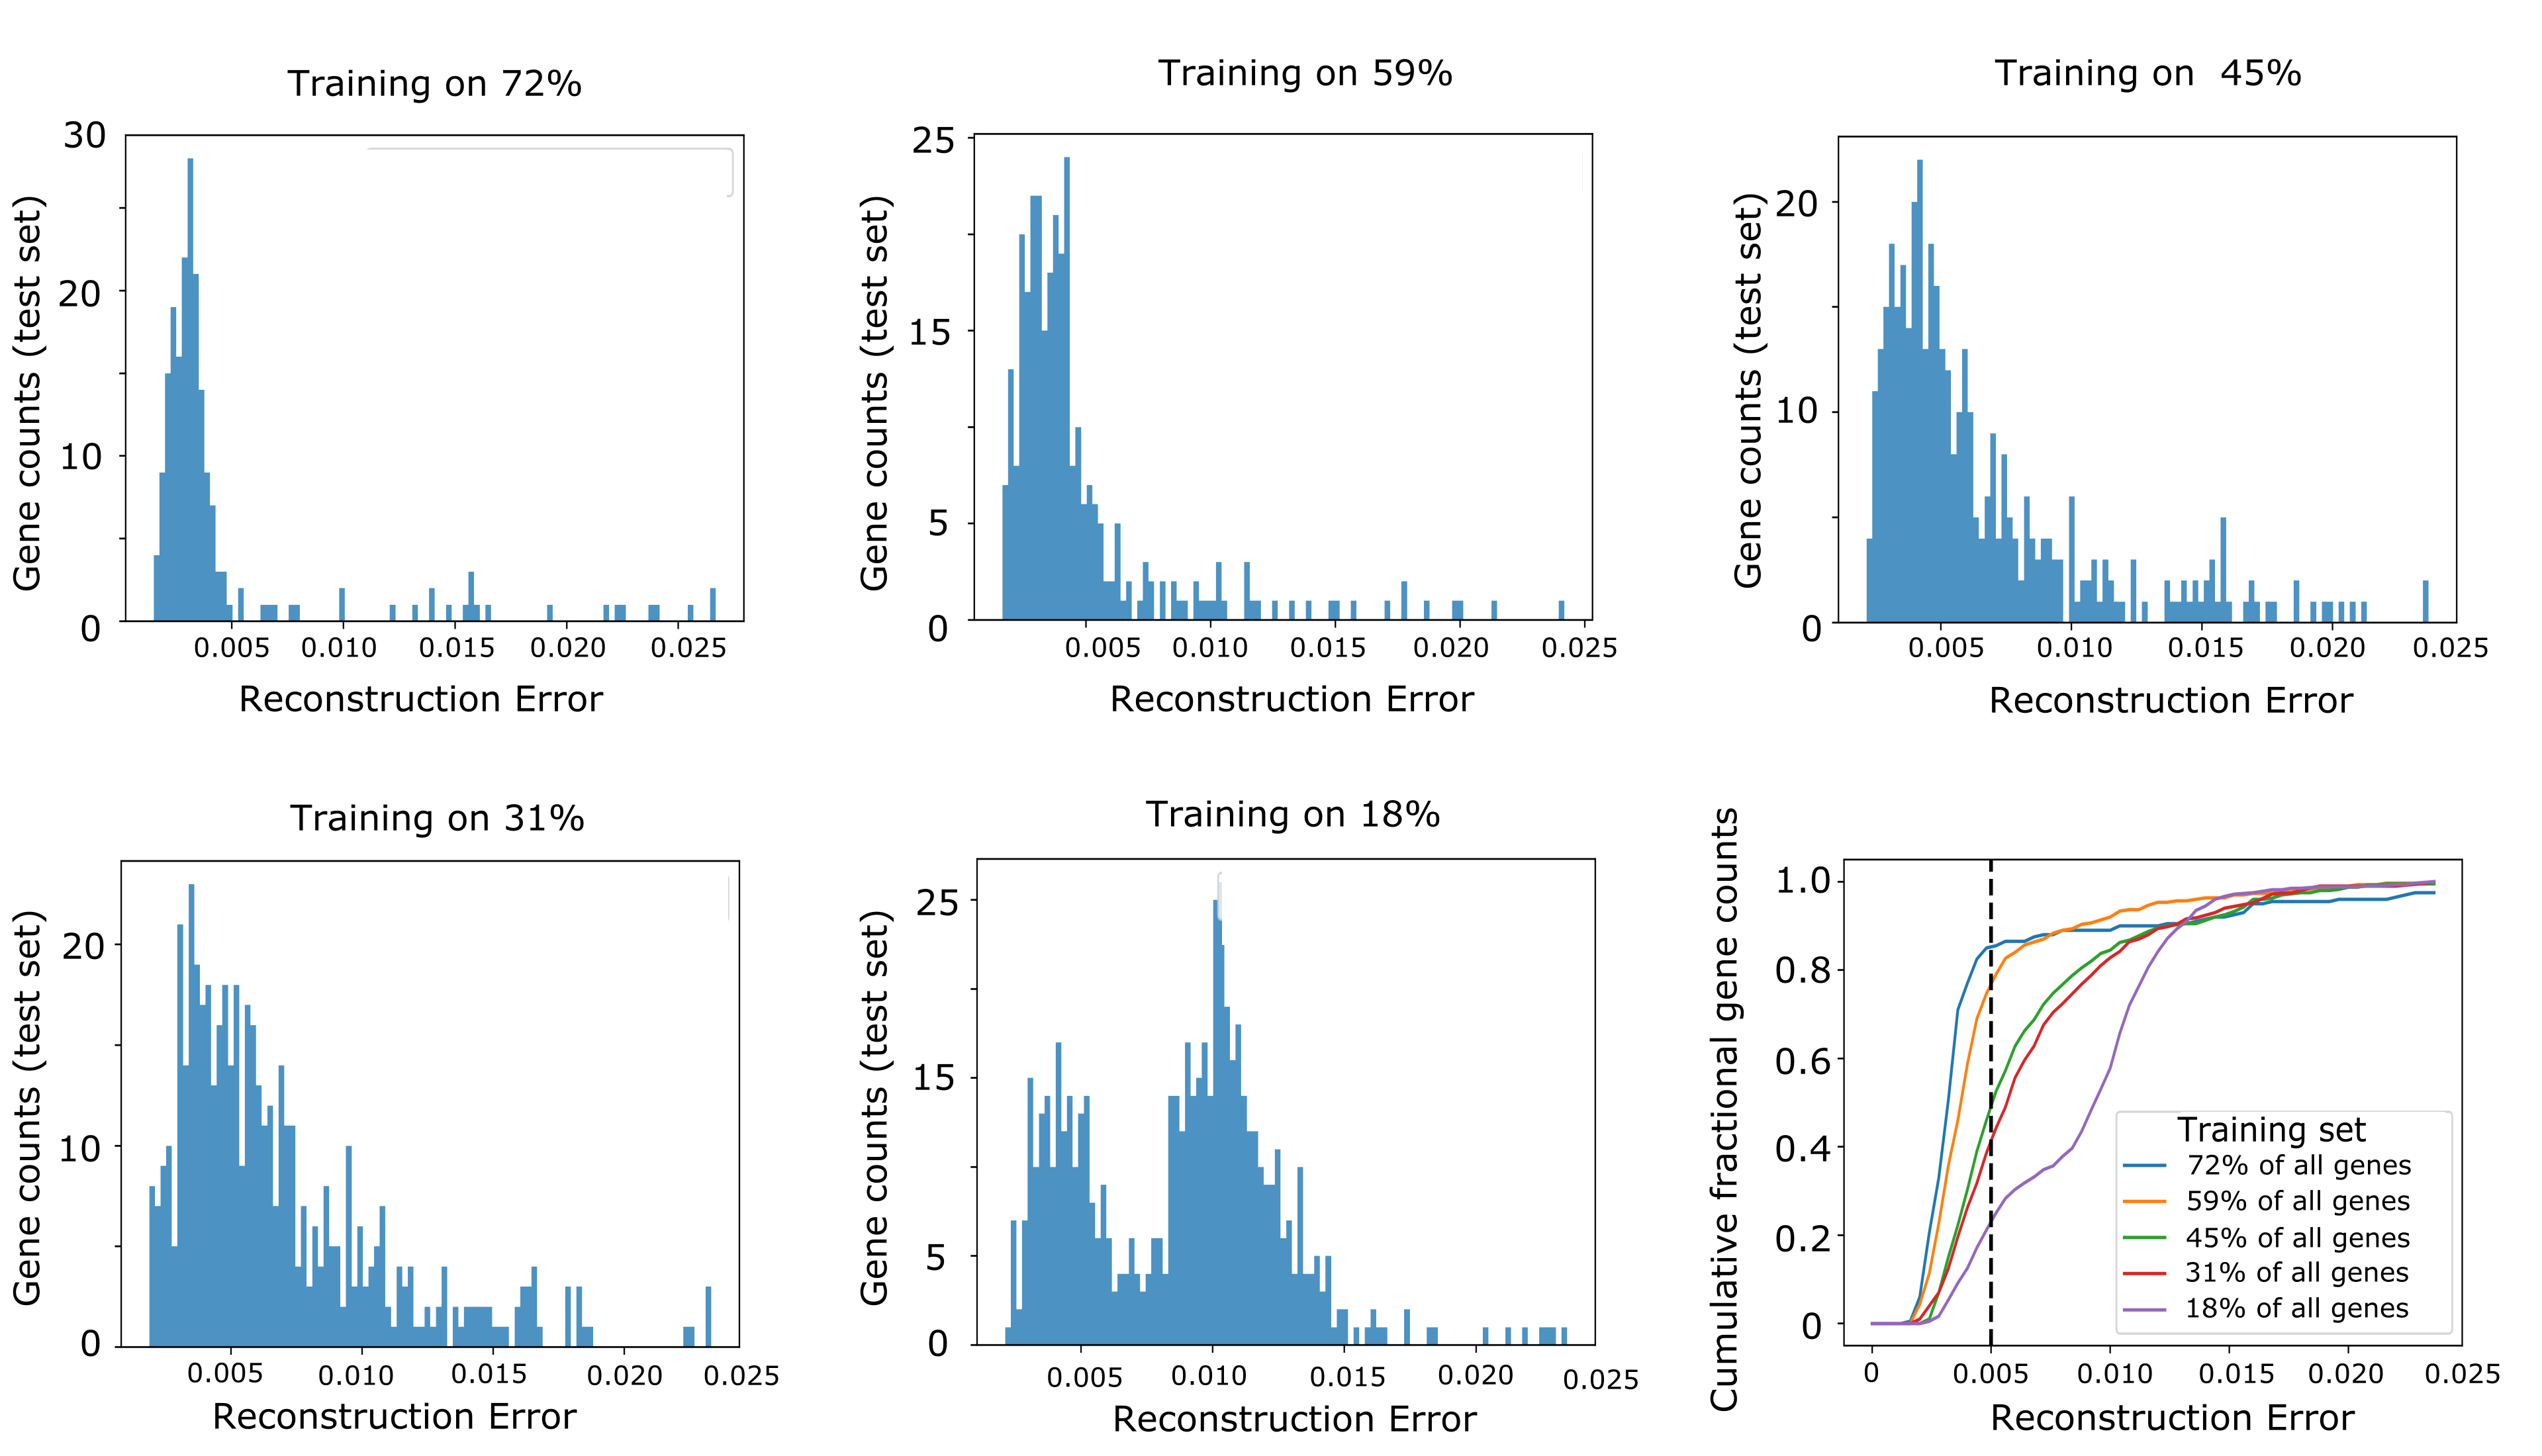
\includegraphics[width=\linewidth]{./figures/supp_varying_test_set_sizes.png}
 % archetecture.png: 1149x508 px, 72dpi, 40.53x17.92 cm, bb=0 0 1149 508
%    \caption{{\bf Accuracy of RVAgene reconstructions for different train/test group sizes.} Distributions of reconstruction errors on randomly sampled sets of test genes, where the full data were split into test groups of: 200 genes (train on 72\%), 300 genes (train on 59\%), 400 genes (train on 45\%), 500 genes (train on 31\%), and 600 genes (train on 18\%). Cumulative fractional distribution of reconstruction errors (cumulative count/test set size) for all groups.}
%  \label{fig:fig5}
%\end{figure}
%}


\subsection{Comparison of RVAgene with alternative approaches for gene clustering}

In order to assess the performance of RVAgene for gene clustering and biological discovery, we compared it to five alternative methods: two neural network approaches and three hierarchical clustering methods. To assess the utility of the recurrent architecture of RVAgene, we trained non-recurrent (i.e. fully connected) variational autoencoders on the embryonic stem cell differentiation dataset \citep{Klein2015}. We compared two options: using the pseudotemporally ordered and smoothed data as input (same as for RVAgene), or using the raw (i.e. unordered and unsmoothed) gene expression data as input. We trained encoder and decoder networks of depth two (one hidden layer) and with a hidden layer size of 400 (we performed a hyperparameter search to optimize this). Theoretically, depth two networks are large enough to learn any non linear function \citep{cybenko1989approximation, hornik1989multilayer, funahashi1989approximate, barron1994approximation}, although the fully connected VAE has no recurrent inductive bias. Thus we test how important this recurrent inductive bias is in practice. 
\par 
The results of the comparison of neural networks are given in \hyperref[fig:fig4]{fig. 6.3A-B}. In
each case, models were trained for 200 epochs. Annotating the results in latent space using
correlations against pseudotime (\hyperref[fig:fig4]{fig. 6.3A}) shows that all three models
separate the data reasonably well, with slightly better separation for the recurrent architecture
(RVAgene). We also annotated the results using cluster labels from the largest four DPGP clusters
for comparison. These are appropriate ``gold-standard'' cluster labels since robust dynamical
signatures are learnt by DPGP in each case (\hyperref[fig:figS3]{Fig. S18}). RVAgene captures: 1) better
separation between clusters that either of the non-recurrent networks, and 2) a spectrum of
behaviors from up- to down-regulated (\hyperref[fig:fig4]{fig. 6.3B}).
\par 
We also performed hierarchical clustering on the pseudotemporally ordered and smoothed data using
three standard hierarchical clustering methods: the Nearest Point Algorithm, the Farthest Point
Algorithm, and UPGMA (the Unweighted Pair Group Method with Arithmetic mean). We annotated the
results with the same clusters labels from DPGP (\hyperref[fig:fig4]{fig. 6.3C}). UPGMA performs best out of these three clustering algorithms, yet still does not attain clear separation between each of the four groups. Thus, the 2D latent space representation of RVAgene is better than both 1D representations via hierarchical clustering and the alternative neural network latent space representations at distinguishing between dynamic gene profiles in pseudotemporally-ordered data.






{\centering
\begin{figure}
  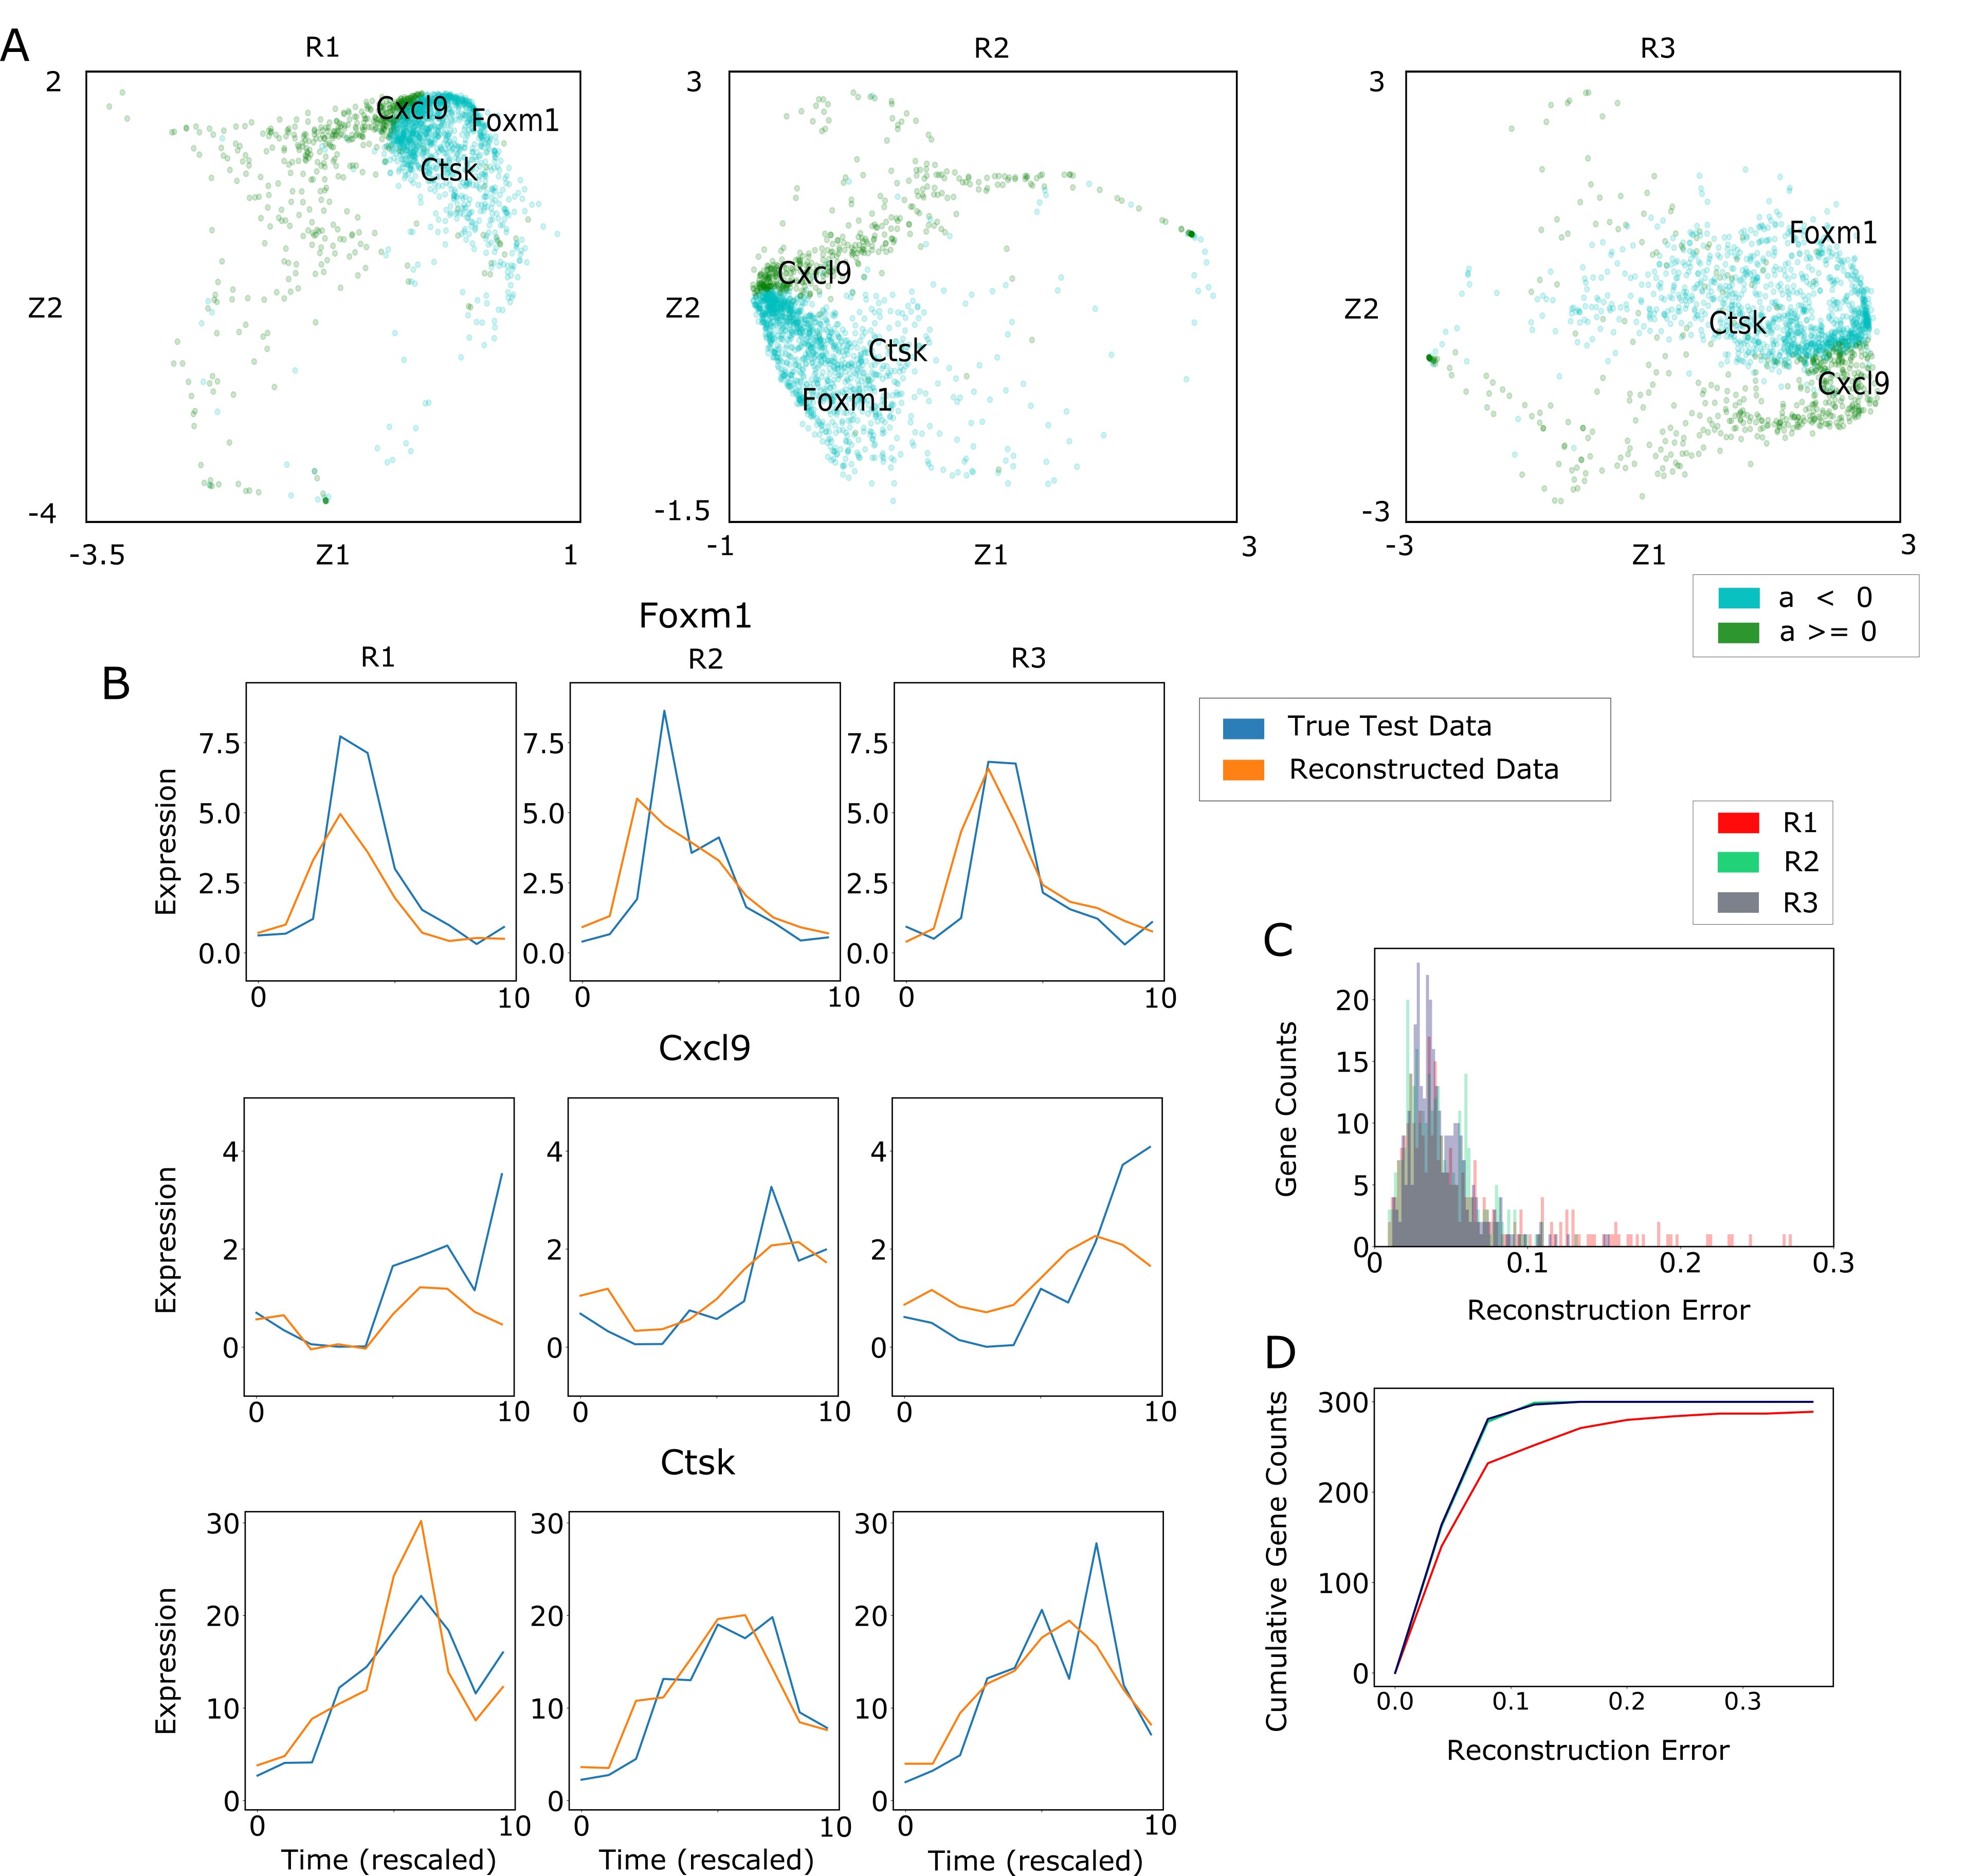
\includegraphics[width = \linewidth]{figures/quad_jci.png}
 % archetecture.png: 1149x508 px, 72dpi, 40.53x17.92 cm, bb=0 0 1149 508
    \caption[Accurate reconstruction of kidney injury response gene dynamics with RVAgene.]{{\bf Accurate reconstruction of kidney injury response gene dynamics with RVAgene. (A)} Latent space representations of RVAgene models trained separately on three independent replicates (R1-R3); classified by quadratic fit coefficient $a$. ({\bf B}) Model generation of gene dynamics for genes not used in training: {\em Foxm1, Cxcl9} and {\em Ctsk}. ({\bf C}) Histograms of reconstruction errors for RVAgene models trained on R1-R3 (truncated). ({\bf D}) Cumulative distribution of reconstruction errors. }
  \label{fig:fig6a}
\end{figure}
}



\subsection{RVAgene can classify and predict gene expression dynamics in response to kidney injury}

We investigated gene expression dynamics in the murine kidney by applying RVAgene to a dataset that describes gene expression profiles before, during, and after a kidney injury \citep{liu2017molecular}. The dataset is temporally rich, with a total of ten bulk samples over twelve months. Since in this case no single-cell information is available, we cannot order samples by pseudotime to smooth the data. Moreover, the temporal gene expression profiles described in \citet{liu2017molecular} display more complex dynamics than for the previous dataset \citep{Klein2015}, and are not readily separable by linear patterns of up- and down-regulated genes (cf. \hyperref[fig:fig3]{Fig. 2C}). Thus, below, we must consider nonlinear models in order to characterize the temporal patterns observed.
\par 
The data consist of one initial timepoint ($t = 0$) before the injury event (an ischemia/reperfusion injury model) and nine subsequent time points ($t = 1$ to $10$) following the injury (48 hours, 72 hours, 7 days, 14 days, 28 days, 6 months and 12 months). We note that the timepoints are not uniformly spaced, which is not taken into account in RVAgene, which only models the broad temporal trend (see Discussion). From an initial list of 1927 differentially expressed genes measured over the time course in three biological replicates, we removed putative/predicted and non-protein coding genes, retaining a list of 1713 genes as input to the model.
\par 
We ran RVAgene separately for each of three biological replicates. Independent replicates \& independently trained models provide additional means with which to test the reproducibility of these methods. For each replicate, RVAgene was trained with a two-dimensional latent space and a hidden size of 10, on the full set of genes over 200 epochs: found to be sufficient for the convergence of $\cL$ (see Methods for further details). We fit linear regression models to the temporal gene profiles (\hyperref[supp]{Fig. S5}) and found that linear fits rarely described the gene temporal profiles well (most correlation coefficients had values close to zero), not did they identify separate clusters in the latent space. Normalizing the data to lie in $[0,1]$ improved our ability to discriminate clusters in the latent space (\hyperref[supp]{Fig. S5C}), but came at the expense of a significant loss of information, as the variance captured in the latent space was dramatically reduced. The absence of evidence for linear correlations could indicate expression dynamics that are uncorrelated with time, but could of course also indicate more complicated (nonlinear) gene expression dynamics, which are explored below. 
\par
To study nonlinear gene expression dynamics, we fit a 2nd degree polynomial, i.e. we fit the temporal trajectory of each gene $x$ to:  $x = at^2 + bt + c$, where $a,b,c$ are constants (\hyperref[supp]{Fig. S6}). We hypothesized that this function could adequately describe the transient dynamics observed by \citet{liu2017molecular} for most genes in response to the kidney injury. 
% Our hypothesis was that this model would be sufficient to capture simple patterns commonly observed during and following kidney injury, where the expression of a gene either increases or decreases transiently, before returning to near-baseline expression values.
Thus, we classified genes into one of two groups, $a < 0$: convex (up-down pattern), 1200 genes; and $a \geq 0$: concave (down-up pattern), 512 genes. In the latent space, the separation of these two groups is clearly visible for each replicate (\hyperref[fig:fig6a]{Fig. 4A}). Moreover, the classification is in agreement with \citet{liu2017molecular}, where the majority of differentially expressed genes are upregulated transiently. 
To explore the ability of RVAgene to reconstruct gene expression profiles not used in model development, we kept aside 300 randomly sampled genes for testing, and trained RVAgene models on the remaining genes for each of the three replicates. Independently for each model, we then generated dynamic profiles for the test genes. Three genes sampled randomly from the test set are plotted in \hyperref[fig:fig6a]{Fig. 4B}. Of particular note, for each of genes, the model-generated data captures the temporal patterns while displaying a higher degree of similarity across replicates than the experimental data itself. This illustrates that the model is neither under- nor overfitting, but capturing the underlying biological patterns while sufficiently accounting for the noise. 
%An interesting point to note is that for each of the shown example genes, the three separately trained RVAgene models for the three replicates come up with similar looking reconstructions although the actual data of the three replicates have different variations (while conforming with the general dynamics common to the three replicates).
Reconstruction errors are comparable across the three replicates, albeit with slightly higher overall errors in replicate 1 (\hyperref[fig:fig6a]{Fig. 4C-D}). Overall, the reconstruction errors are higher than for the previous section (averaging over many pseudotemporal time points allowed us to significantly reduced the noise). 



{\centering
\begin{figure}
  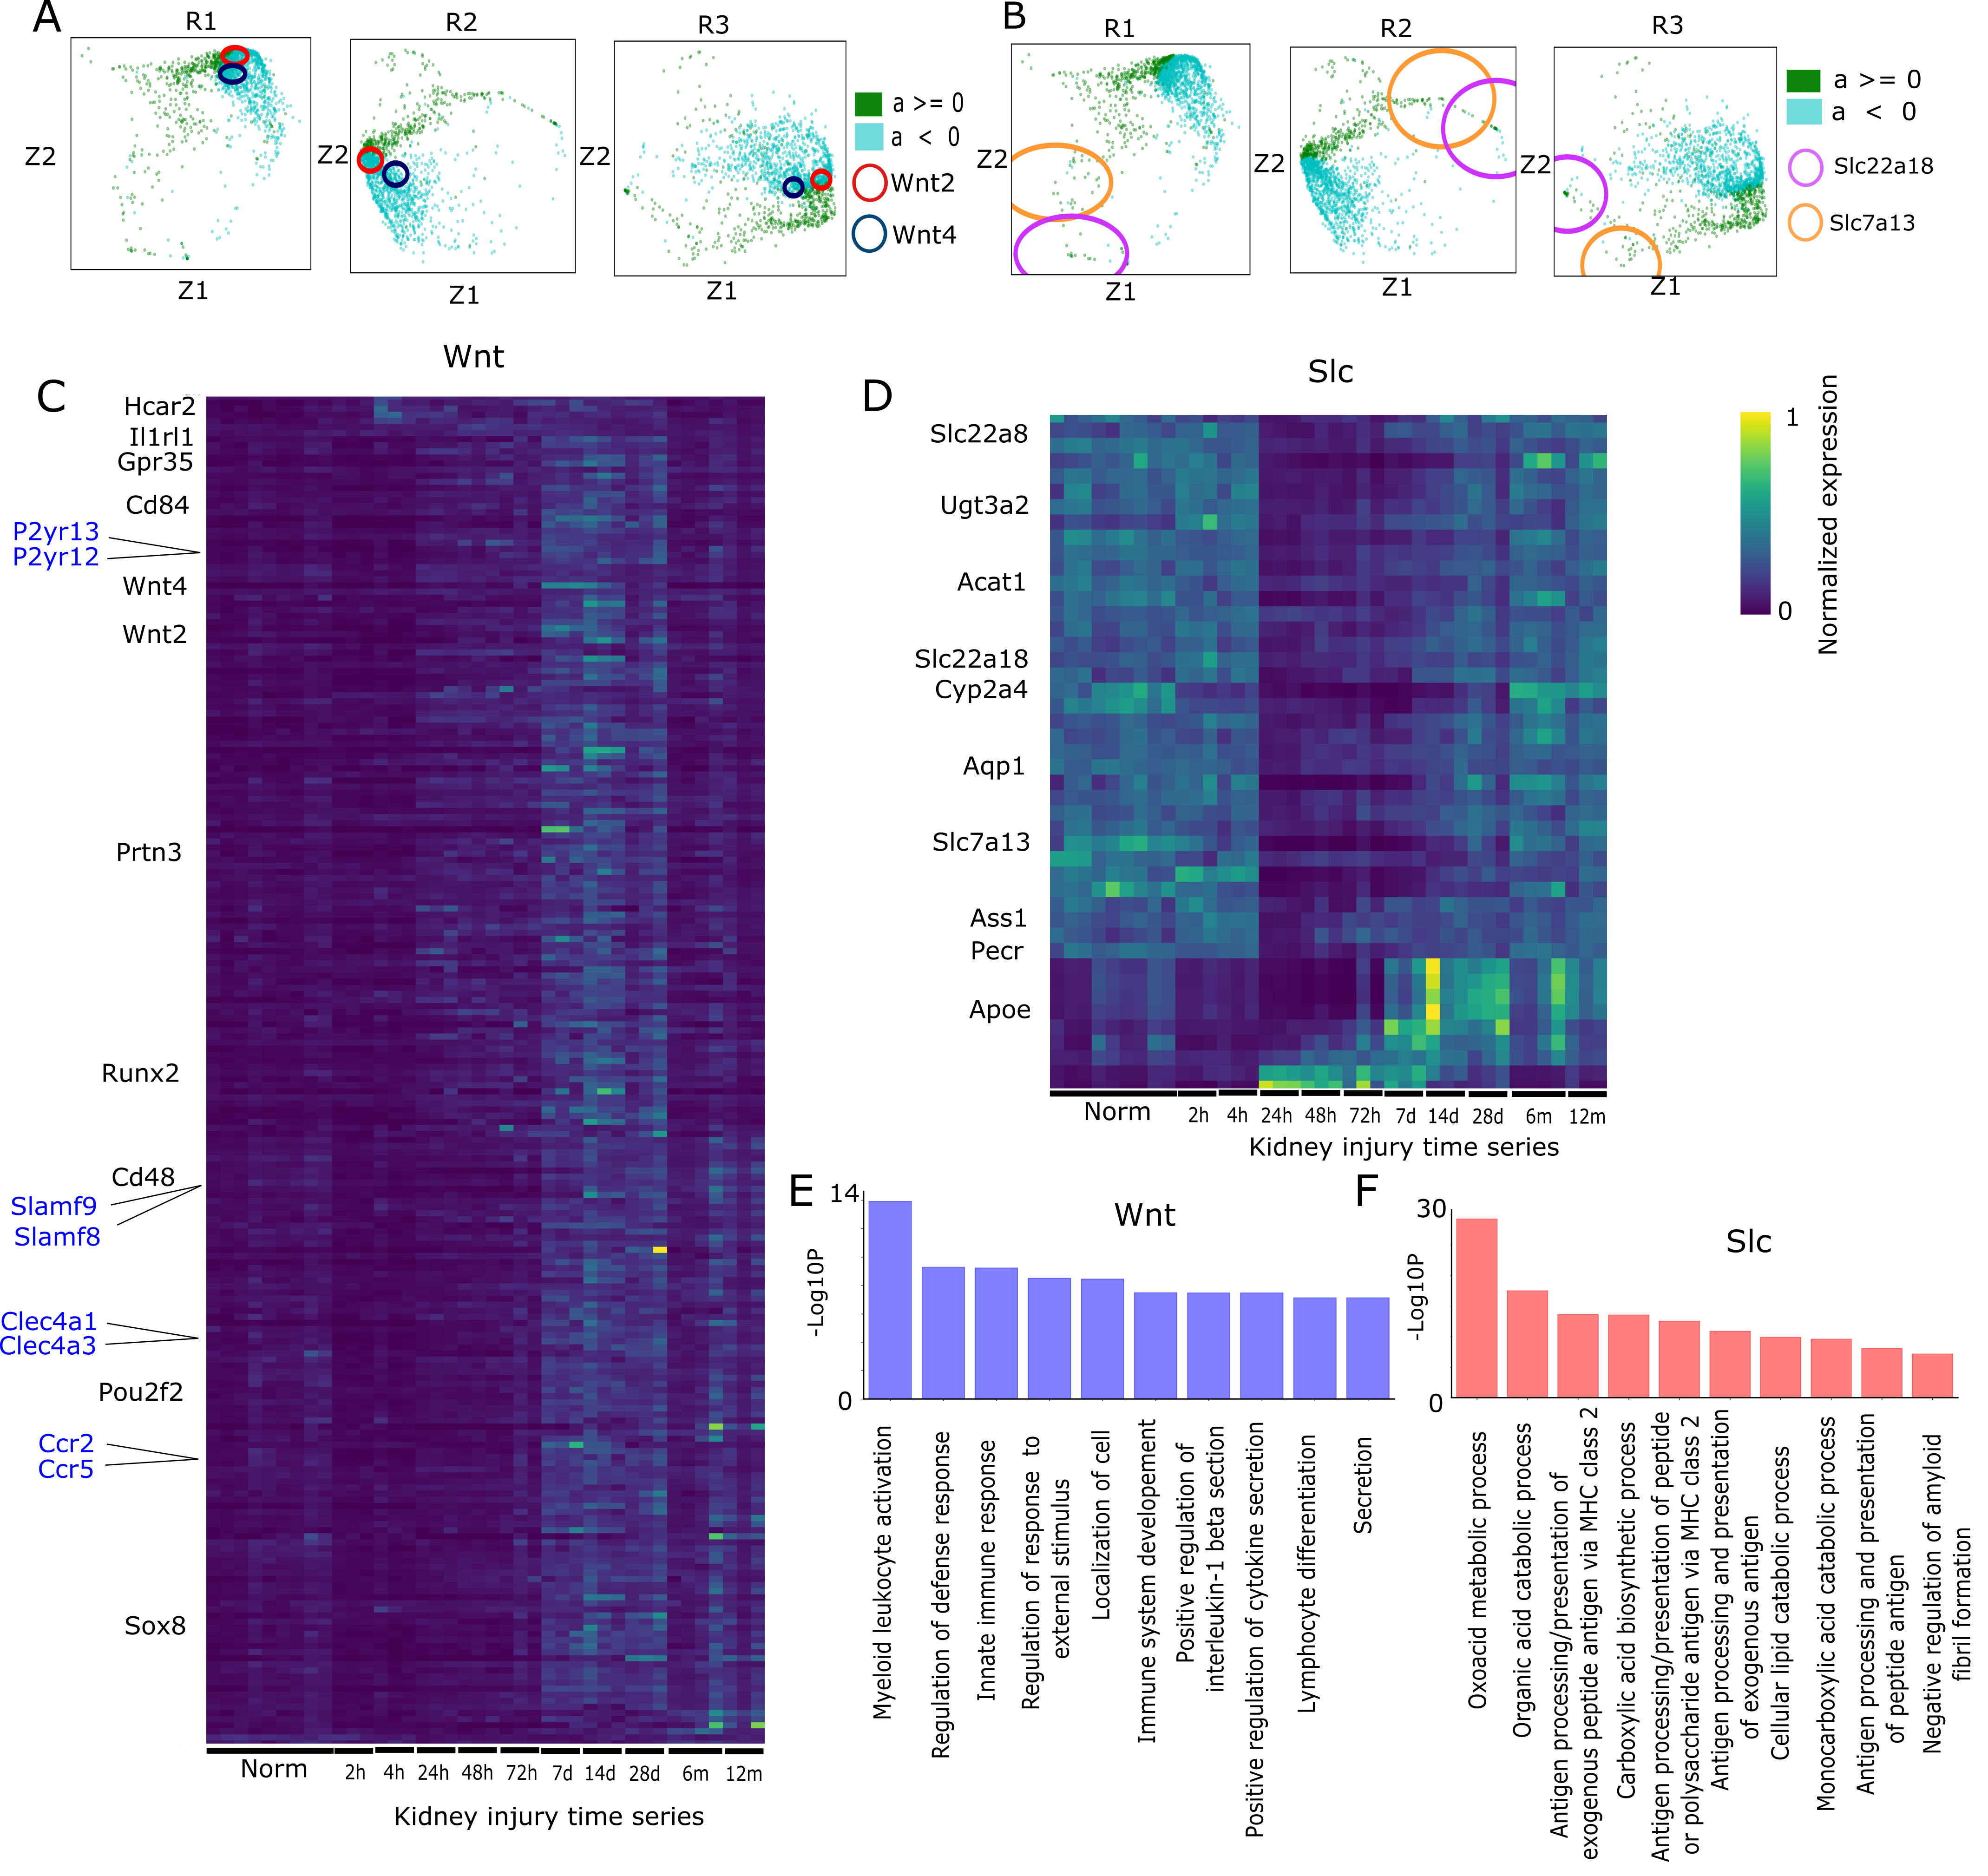
\includegraphics[width = \linewidth]{figures/fig9.png}
 % archetecture.png: 1149x508 px, 72dpi, 40.53x17.92 cm, bb=0 0 1149 508
    \caption[RVAgene latent space captures biological processes driving concordant gene expression changes.]{{\bf RVAgene latent space captures biological processes driving concordant gene expression changes. (A)} Z-plots for replicates R1-R3 with local neighborhoods of Wnt2 and Wnt4 marked (circles). ({\bf B}) As in A, for Slc family members Slc22a18 and Slc7a13. ({\bf C}) Heatmap of expression changes over time course of injury for the Wnt neighborhood genes in the intersection of R1-R3. Selected genes marked (black), as well as ortholog gene pairs (blue).  ({\bf D}) As in C, for Slc neighborhood genes. ({\bf E}) Histogram of -log10 p values of gene ontology terms for biological processes terms associated with the Wnt neighborhood (gene set in C). ({\bf F}) As in E, with the Slc neighborhood (gene set in D). }
  \label{fig:fig6b}
\end{figure}
}

{
  To investigate in more depth the features that are captured in the RVAgene latent space, we performed two sets of analyses: unbiased clustering, and targeted exploration. For the unbiased analysis, we performed k-means clustering on RVAgene latent space of replicate 1 (R1) with $k=9$ (Supplementary \hyperref[supp]{Fig. S7A}); we project the clusters labels learnt onto replicates R2 and R3. All cluster identities are well-preserved across replicates, with the exception of cluster 5, which seems to indicate outlier genes in R1. To study biological processes within these clusters, we performed GO term enrichment analysis on each. In Supplementary  \hyperref[supp]{Fig. S7B} we plot one significant GO term per cluster (omitting cluster 5), and see that specific regions of the latent spaces across replicates can be characterized in terms of biological processes, many of which relate to metabolic and immune system responses. These can be separated into two broad classes, which separate the left-hand side of R1 (metabolic processes downregulated during injury response) from the right-hand side (immune responses upregulated during injury response). 
}
\par 
To study the effects of gene-specific regions of the latent space in greater depth, we chose three distinct regions based on the co-location of genes of interest. These gene groups studied on the latent space are: 1) a {\em Wnt} group consisting of family members {\em Wnt2} \& {\em Wnt4}; 2) an {\em Slc} group consisting of family members {\em Slc7a13} \& {\em Slc22a18}; and 3) a {\em Sdc1} group, consisting of only {\em Sdc1}. For each group, we characterized neighboring genes by defining a circular neighborhood around each gene in the group, with radius $r$ (depending on the local density, the radius was varied, giving: $r^2 = 1$ for {\em Slc}, $r^2 = 0.3$ for {\em Sdc}, $r^2 = 0.05$ for {\em Wnt}. We then took all genes inside this radius for each replicate, and found the intersection of genes over the three replicates (\hyperref[fig:fig6b]{Fig. 5A-B}). We analyzed the intersection gene set for each group by studying their temporal profiles and their gene ontology (GO) term associations. Each group was characterized by a strikingly clear temporal profile. The {\em Sdc1} and {\em Wnt} groups both show transient upregulation, over different timescales: the {\em Sdc1} group is upregulated from 24 hours post-injury until 14-28 days post-injury (fast response) (Supplementary \hyperref[supp]{Fig. S8B}), whereas the {\em Wnt} group is upregulated at 7 days post-injury until 28 days post-injury (slow response) (\hyperref[fig:fig6b]{Fig. 5C}). In contrast, the {\em Slc} group is downregulated at 24 hours post-injury, and remains suppressed until 7-28 days post-injury (\hyperref[fig:fig6b]{Fig. 5D}).
\par 
Analysis of GO biological process terms enriched in each gene group further highlighted the power of the latent space for biological discovery. The fast response ({\em Sdc1}) group was characterized by upregulation of programs related to apoptosis, stress response, wound healing and chemotaxis, i.e. the first responders to the site of injury (\hyperref[supp]{Fig. S8C}). In addition all five {\em Lox} genes comprising the GO term ``peptidyl-lysine oxidization'' were found in this group. This is consistent with the oxidative stress resulting from the renal ischemia-reperfusion injury that was performed. However, distinct factors regulate the {\em Lox} family genes, as can be partly observed by their subtle differences in temporal profile (\hyperref[supp]{Fig. S8D}). Their co-location in the latent spaces of all three models thus highlights the potential use of RVAgene for discovery of complex temporal regulatory events from gene expression data.
\par
The slow response ({\em Wnt}) group was primarily characterized by immune response processes, including leukocyte activation, platelet aggregation, and various cytokine-mediated pathways including {\em IL-1} and {\em IL-33} (\hyperref[fig:fig6b]{Fig. 5E}). Notably, the Wnt group identies multiple gene orthologs (\hyperref[fig:fig6b]{Fig. 5C}) with very similar profiles: likely evidence of shared temporal regulation. This illustrates once again (as for the {\em Lox} genes above) the potency of RVAgene for the discovery of temporally co-regulated genes.
\par
Finally, the {\em Slc} group of genes shows a transiently down-regulated pattern between 24 hours and 7-28 days, although some gene in this group deviate from this pattern (\hyperref[fig:fig6b]{Fig. 5D}). 
GO term enrichment identifies the positive regulation of metabolic processes (\hyperref[fig:fig6b]{Fig. 5F}). The downregulation of metabolic programs during the response to kidney injury is agreement with the findings of \citet{liu2017molecular}. Notably, this metabolism-sensitive group contains many genes that also display sexually dimorphic expression, primarily in specific regions of the proximal tubule \citep{ransick19_singlecell}, thus independently identifying the well-established (though under-studied) interplay between sex differences and injury responses in the kidney \citep{neugarten00_effect}. 
\par 
In summary, unsupervised analysis of groups of genes co-located in the latent spaces of RVAgene finds: 1) high similarity between temporal gene profiles of genes nearby in latent space, and 2) clear biological signatures represented by these groups of nearby genes, in strong agreement with prior knowledge \citep{liu2017molecular}. Moreover, the latent spaces of RVAgene models can be used to predict programs of temporal co-regulation. 
\par


% In the latent space representation for all those genes and for the three replicates. We can see genes with positive and negative correlation between expression and time axis are not as distinctly separated as previous section, which is expected (Supplementary \hyperref[supp]{Fig. S2-B}). 
% This also hints that this dataset might not have clear cluster structures and an uninformed clustering effort on this dataset might produce forced spurious results. Now, one might think that the correlation measure is a measure of shape and somehow magnitude of expression of genes is playing part here (i.e. may be genes with similar dynamics but different scale of magnitudes are being viewed differently). Which means, normalising the expression magnitudes across timepoints to the same range (e.g. 0-1) might be helpful to increase the clarity of separation between the red and blue class. This indeed works as can be seen in supplementary \hyperref[supp]{Fig. S2-C}. However, it drastically reduces the variance in the latent space which can be inferred from the hugely shrunken scales of the axes from supplementary \hyperref[supp]{Fig. S2-B} to supplementary \hyperref[supp]{Fig. S2-C} for both dimensions of latent space i.e. a lot of important information is lost. This might not be a problem for the representation learning part, but, it means the decoder will be hugely underfit. So, we do not recommend normalising the data without any solid reason for the same. Another possibility is increasing the dimension of latent space. A 3D latent space could be better in this case but increasing it beyond 3 defeats the purpose of representation learning because each gene has only 10 timepoints anyway and latent space with more than 3 dimension will require dimensionality reduction for visualization.
 
%%% Local Variables:
%%% mode: latex
%%% TeX-master: t
%%% End:


\begin{center}
    \begin{figure}
    \makebox[\textwidth]{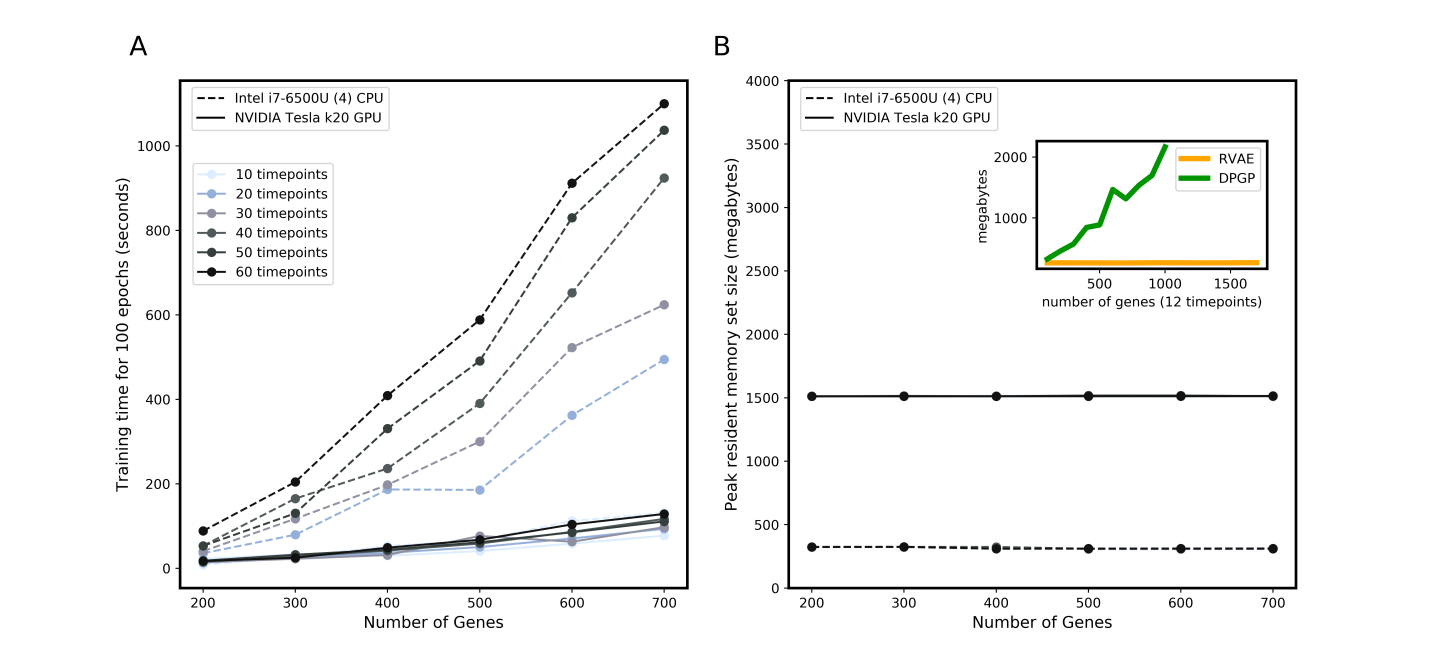
\includegraphics[width=0.8\paperwidth]{figures/fig7.png}}
 % archetecture.png: 1149x508 px, 72dpi, 40.53x17.92 cm, bb=0 0 1149 508
        \caption[Computational cost of training RVAgene]{\textbf{Training RVAgene is reasonably scalable on CPU and even more so using hardware acceleration through GPU.} ({\bf A}) Time cost of training RVAgene for 100 epochs for datasets with varying number of genes and time points on CPU and GPU. ({\bf B}) Maximum memory utilized during training of the model on CPU an GPU for the cases in (A), inset plot: comparison of max memory used compared to DPGP for varying number of genes.}
  \label{fig:fig7}
\end{figure}
\end{center}


\subsection{Assessment of the computational efficiency of RVAgene}

We assessed the computational efficiency of RVAgene for various settings and hardware. For the
majority of the models trained, 100-200 epochs was sufficient for the loss function $\cL$ to
converge. For tests performed here, we recorded the RVAgene runtime for 100 epochs of training using
models that varied in their number of genes and time points. In each case we used a latent space of
dimension two, a hidden size of 10, and a training batch size of 10. We ran the model on an intel i7
CPU with four cores and a Tesla K20 GPU. Runtimes were recorded on linux via the inbuilt time script
(\texttt{/usr/bin/time --verbose}). As the number of time points and genes grew large (up to 60 time
points and 700 genes), total runtimes on CPU were on the order of $10^3$ seconds ($<$ 20 minutes)
(\hyperref[fig:fig7]{fig. 6.6A}). On GPU, total runtimes were decreased to around $100$ seconds ($< 3$ minutes). Thus, RVAgene is readily scalable to tens of thousands of genes and hundreds of time points for training times of up to a few days on CPU or hours on GPU. For comparison, as described in \citet{McDowell2018}, the approximation-free time complexity of each iteration of learning for DPGP is $\cO(GT^3)$, due to the $G$ matrix inversions, each of size $T \times T$, for a dataset with $G$ genes and $T$ timepoints. The complexity for each epoch of training of RVAgene is $\cO(GT)$.
%The cubic complexity of the hierarchical Gaussian Process learning in DPGP quickly increases training time and does not allow scalability over timepoints without some form of approximation.
\par 
In terms of peak memory usage, since RVAgene is a neural network trained using backpropagation
\citep{rumelhart1986learning}, maximum memory used during training is of the same size as the
network itself, which is constant given that the model parameters are fixed
(\hyperref[fig:fig7]{fig. 6.6B}). This is in contrast to Gaussian Processes (such as DPGP), which
initially assign each gene to its own cluster, thus must store $G$ matrices of size $T\times T $,
for $G$ genes and $T$ timepoints per gene. This leads to quickly increasing runtime peak resident
set sizes for DPGP compared to RVAgene (\hyperref[fig:fig7]{fig. 6.6B} Inset). The memory used by DPGP grows with the number of time points as $\cO(GT^2)$). Thus, DPGP will not run with large numbers of genes and time points. %, and RVAgene has greater potential for the discovery of nuanced dynamical features in the data.
A note on this comparison: it is not direct, in the sense that DPGP performs clustering and RVAgene does not, in addition to other important differences between the goals of the methods. 
%However, we must add that direct comparisons must be made cautiously, given the differences between the two methods. 
%DPGP performs independent gene clustering; RVAgene does not (clustering can be performed downstream on the latent space).
Nonetheless, the size and scope of current biological datasets -- particularly at single-cell resolution -- in many cases preclude the use of DPGP without large reductions of the input data size. As we have shown, a feasible and efficient alternative in such cases is to run RVAgene, and then to perform clustering or other classification analyses post hoc on the latent space of the model. 


%what does it do?
%- visualization/classification (encoder) and prediction/generation (decoder)
%
%Plan
%- overview of main findings - ability to classify, predict, and generate 
%- current uses - tuning hyperparameters (DPGP) 
%- current uses - interpretability (cf. other VAEs)
%- future uses - interpretability - using LDVAE
%- future uses - (GRNs)
%- future work: time interval 
%- future work: discret time 
%- future work: different priors (cite SOUP)
%- conclusion


\section{Discussion}
{We have presented RVAgene, a recurrent variational autoencoder for generative modeling of gene expression time series data.
Through its encoder network, RVAgene provides means to visualize and classify gene expression dynamic profiles, which can lead to the discovery of biological processes.
Through its decoder network, RVAgene provides means to generate new gene expression dynamic profiles of either the full data or (in the case of single-cell studies) the pseudotime-smoothed data by sampling points from the latent space. In doing so, RVAgene can accurately reconstruct gene dynamics in complex biological data. As a by-product, on single-cell datasets the model directly produces smoothed outputs, useful for denoising gene expression time series data. RVAgene is efficient on temporally-rich whole genome datasets, in comparison to current existing methods. }
\par
RVAgene can be used to discover structure in the data, such as gene profile clusters. Popular
methods for clustering gene profiles such as Bayesian hierarchical clustering
\citep{cooke2011bayesian} or DPGP \citep{McDowell2018} detect the number of clusters in the data by
fitting a hyperparameter $\alpha$, the concentration parameter of the governing Dirichlet process
\citep{ferguson1973bayesian}. Although unsupervised, inevitably, the choice of $\alpha$ affects the
number of clusters output. Visualizing the data first with RVAgene can give an idea whether the data
favor clustering or a continuous representation. Thus analysis in RVAgene can guide the setting of
the hyperparameter $\alpha$ in DPGP and similar methods. In the case of ESC differentiation, DPGP
predicts 12 clusters (\hyperref[supp]{ Fig. S3}), yet most have very few members and many share
similar patterns. The RVAgene latent space for this dataset finds two major divisions in the data,
and orders the largest DPGP clusters along a spectrum (\hyperref[fig:fig3]{Fig. 1.2D}), suggesting that DPGP might be overfitting the data. Indeed, the two methods can be used complementarily: RVAgene for high-level structure discovery and DPGP for clustering.
{In cases where learning a detailed noise model (at single time point resolution) is important to the user, DPGP or other Gaussian Process models are preferable over RVAgene.}
However, DPGP does not scale well with large datasets and thus cannot always be used
(\hyperref[fig:fig7]{Fig. 1.6}).
\par 
The latent space of an RVAgene model encodes useful information about biological features, and in that sense provides biologically interpretable representations of the data. However, the representation is not interpretable in the sense that the components of the latent space do not have a physical meaning nor are they necessarily independent. Recent methods have tackled this issue of interpretability, by either modifying the loss function to make components independent \citep{higgins2016beta} or substituting linear functions in parts of the VAE \citep{svensson2020interpretable, ainsworth2018oi}. These methods have clear advantages regarding the analysis and interpretation of features in the latent space. In future work, decoding an RVAgene model with a linear function \citep{svensson2020interpretable} could facilitate additional discovery and improve our ability to gain insight into dynamic biological processes through the analysis of the latent space.
\par 
Dynamic changes in gene expression underlie essential cell processes. As such, modeling gene expression changes can also facilitate downstream analysis tasks, including gene regulatory network (GRN) inference. Inferring gene regulatory networks from single-cell data is challenging \citep{chen18_evaluating}, particularly due to cell-cell heterogeneity and high levels of noise. Several recent approaches to GRN inference make use of temporal profiles \citep{deshpande19_network, kim20_tenet}  
or differential equations \citep{ma20_inference, aubin-frankowski20_gene, matsumoto17_scode}. RVAgene could supplement such methods either by providing denoised input data, or by completely replacing the temporal ordering/differential equation-based components of these methods (which can be notoriously difficult to parameterize) with data produced from a RVAgene generative model of the gene expression dynamics.
\par 
RVAgene is currently agnostic of irregular time intervals between consecutive points in a time series,  i.e. it standardizes the time interval. This is not usually a concern for single-cell data, since with pseudotime information we can choose appropriate time intervals. However, in other cases, such as in response to kidney injury \citep{liu2017molecular}, standardizing time intervals distorts the dynamic profiles. Since RVAgene seeks to describe broad temporal patterns, we do not see this as a critical issue, though it would be desirable to generalize the model. A simple way to model irregularly spaced time points would be to augment the data through interpolation, though this is difficult without making strong assumptions about the (generally unknown) noise model. Gaussian process models \citep{McDowell2018, hensman2013hierarchical} can take irregular data as input, although (as noted above) are not efficient enough to run on large datasets. An alternative approach would be to modify the recurrent network architecture to take time points explicitly as input values, this would enable modeling of irregular or asynchronous data \citep{wu2018modeling}.
%\tcr{ https://link.springer.com/article/10.1186/1471-2105-14-252}
\par
RVAgene models in discrete time steps. There is no simple modification to the recurrent network structure that allows for prediction on continuously valued time. However, a recent development: neural ordinary differential equations (ODEs) \citep{chen2018neural}, enables modeling of time series data with continuous timepoints. \citet{chen2018neural} describe a generative latent ODE architecture similar to that of RVAgene, except that in their case the recurrent decoder network is replaced by a neural ODE decoder network. \citet{chen2018neural} demonstrate accurate results using synthetic data, however when we applied the method to the ESC single-cell differentiation dataset \citep{Klein2015}, the neural ODE network was found to converge very slowly and was overall underfit (\hyperref[supp]{Fig. S9}). The latent ODE method used by \citet{chen2018neural} does not address the challenge of modeling asynchronous/irregularly spaced data, but this has been more recently addressed \citep{rubanova2019latent}. These new models may well lead to future improvements in network architectures, although it seems that computational progress is needed before they can be successfully applied to complex biological systems.
%We will keenly follow developments in the field. 
\par 
In the current work, the prior on latent space used throughout was a unit spherical Normal, appropriate for exploratory data analysis where we have no further knowledge about structure in the latent space.
% ($\cN(\mathbf{0},\mathbf{I})$). 
However, given more information, e.g. that the data contains $k$ clusters, a different prior on the latent space might be more appropriate. A multi-modal prior -- such as a Gaussian Mixture Model (GMM) prior -- would permit structured (multi-modal) representations. However, the KL-divergence for an arbitrary GMM is not tractable; approximation  \citep{hershey2007approximating} or numerical computation would be necessary. Moreover, there is a greater problem: mixture models contain discrete parameters and VAE models are ill-suited for the optimization of discrete parameters \citep{dilokthanakul2016deep}, thus directly replacing the Normal prior of a VAE with a GMM is not feasible. A workaround to this problem is presented in \citep{dilokthanakul2016deep}, however implementing this for a recurrent model architecture remains an open problem. 
%A  k-modal prior would increase the probability of a latent space representation containing $\geq k$ clusters, i.e. increasing the structure of the space. 
%cite SOUP
\par 
The points raised above offer much scope for future work. These include the design of new latent space models with informative priors, modeling irregular time series data, and modeling in continuous time. Developments in some of these areas \citep{chen2018neural}, while promising, tend to rely on training data with relatively low levels of noise: far from the reality of most biological data. Thus it seems highly likely to be beneficial for both machine learning and biology to develop new neural network architectures in light of biological data. 











\section*{Acknowledgements}
We thank A.P. McMahon for valuable discussions and comments on the manuscript.
R.M. gratefully acknowledges support from a USC Viterbi Fellowship.

\section*{Data Availability}
The synthetic data used for evaluation of RVAgene are available at:
\url{https://github.com/maclean-lab/RVAgene}. Additional data used in the manuscript are available from the Gene Expression Omnibus: ESC differentiation (GEO accession GSE65525) and kidney injury (GEO accession GSE98622).

\section*{Software Availability}
RVAgene is available in Python released under an MIT license:  \url{https://github.com/maclean-lab/RVAgene}.


%%%%%%%%%%%%%%%%%%%%%%%%%%%%%%%%%%%%%%%%%%%%%%%%%%%%%%%%%%%%%%%%%%%%%%%%%%%%%%%%%%%%%%%%%%%%%%%%%%%%%%%%%%%%%%%%%%%%%%%%%%%%%%%%%%

%%%%%%%%%%%%%%%%%%%%%%%%%%%%%%%%%%%%%%%%%%%%%%%%%% CRF %%%%%%%%%%%%%%%%%%%%%%%%%%%%%%%%%%%%%%%%%%%%%%%%%%%%%%%%%%%%%%%%%%%%%%%%%%%
% More Research Topics
% \include{ResearchTopic2}

\chapter{A probabilistic model for smooth binding site label prediction on protein surfaces}
\label{cha:research_topic_2}

\vspace*{0.35in}

\begin{flushleft}

%{\large Raktim Mitra\textsuperscript{1}, 
%Jared Sagendorf\textsuperscript{1}}\\

%\bigskip
%$^1$Quantitative and Computational Biology, University of Southern California
%\\


\end{flushleft}

\begin{abstract} 
    Predicting DNA/RNA binding sites on a given protein surface is an important computational task, since experimentally determining such information is often expensive and time consuming. This binding site prediction task can be formulated as a node classification task over a 3D mesh representing the protein surface, with features over the vertices and edges of the mesh representing various geometrical and physicochemical features of the protein structure. We developed a deep learning based method, PNAbind, which classifies mesh vertices as binding and non-binding sites. This often results in irregular binding site predictions over the protein surface. However, intuitively, binding site predictions should be contiguous and not patchy i.e. as ``smooth" as possible while being correct. In this chapter, we describe what such kind of ``smoothness" entails and we improve upon the original architecture by designing a network layer based on a probabilistic Continuous Conditional Random Field (CCRF) model, which increases smoothness of binding site prediction while improving prediction accuracy of the model. This network layer implementation has been published as part of the PNAbind package.
\end{abstract}

\section{Introduction} Predicting DNA/RNA binding sites on protein structures is an important
computational task.  There are many existing methods which attempt to solve this problem either on
the sequence level or on 3D structure level based on either sequence features or structural features
of proteins \citep{deng2018pdrlgb, wang2010bindn+, wang2006bindn, li2013predna}
.We  represent protein surfaces as 3D triangulated meshes with 
vertices and edges having features representing diffferent geometrical and physicochemical aspects
of the protein structure. Now, we can learn a model which classifies each vertex of such a mesh to either binding-site or
non-binding sites. With recent advances in 3D deep learning, Graph Convolutional
Networks(GCNs) have come out as a useful approach for learning higher level features over
3D mesh objects. We developed a GCN based deep learning model for the binding site classification
task: Geobind. \hyperref[fig:crf_concept]{Fig. 2.1A} shows schematic diagram of
the task Geobind achieves.

Standard neural network approach is to predict each binding-site label independently
through it's output layer. However, classification tasks often come with additional non-trivialities which
are not addressable with independence assumption.  For example, image segmentation task involves
classifying every pixel of an image (which can be thought of as a grid of pixels) to some class.
However, independence assumption often gives poor/scattered results. In that case, some form of
conditionallabel (re)assignment is necessary for each pixel considering its neighbouring pixels. The
most common way to achieve the same in the field of computer vision is via optimizing a conditional
random  field (CRF) model over a set of initially  learned labels. For example,
\hyperref[fig:crf_concept]{Fig. 2.1B} adapted
from \citet{krahenbuhl2012efficient}  shows how an implementation based on CRF can improve image
segmentatation results. In our case, we also expect certain properties from a predicted binding site
region on a protein surface. A binding site region on a protein surface is basically a combination
of multiple mesh vertices predicted as binding site. We generally expect such a region to be
"smooth" i.e. not randomly have misclassified points scattered around. This idea is visually illustrated in
\hyperref[fig:crf_concept]{Fig. 2.1C}. So, we need to do some kind
of conditional (re)assignment of class labels generated by our Geobind network.

In addition to Computer vision, CRF models are also heavily used in Natural Language processing (NLP)
\citep{roark2004discriminative,mccallum2003early,liu2017identification}. However, both in Computer
vision and NLP, the underlying graph structure, over which the CRF is defined, is very sparse and
simple e.g. linear chain or tree for NLP and 2D grid for computer vision. Which makes it easy to
find some form of optimization scheme on the discrete domain of labels. However, this is not the
case for a general underlying graph, where the combinatoriality of the possible label assignments
for all vertices is huge and in the discrete domain of labels there is no gradient information for
efficient optimization.

\citet{krahenbuhl2012efficient} proposes an efficient inference algorithm for fully connected CRFs
based on mean field Variational Inference and high dimensional filtering using permutohedral lattice
approximation. However, the high dimensional filtering step is not compatible with
SIMD\citep{nickolls2008scalable} paradigm of GPU computation. \citep{teichmann2018convolutional}
making it impossible to use on large datasets and non-trivial graphs.
\citet{teichmann2018convolutional} improves upon this by implementing Convolutional CRFs which is
another kind of approximation to full CRF inference which is efficient and compatible with GPUs.
However, their method is only applicable for 2D grid i.e. image data.  However, none of these methods
are applicable to our case directly. One of the more interesting advances of applying CRF layer on
mesh object comes from \citet{kalogerakis2010learning} using alpha-expansion graph-cuts method proposed by
\citet{boykov2001fast}. However, being pre-CNN revolution work, this method is not sutiable for deep
learning and is not readily integrable to our Geobind model. 
\par
Overall, it turns out, optimizing a CRF model over the predicted labels of Geobind on the discrete
domain to reassign them is not computationally easy. However, instead of trying to smooth the
predicted labels we can directly try to make these predicted labels itself smoother. This means we
need to have an operation before the final fully connected layer of Geobind which smooths the
information over different vertices taking into account their neighbours information along with
their own. The good thing about this idea is that the optimization domain is not discrete anymore.

Such an operation is based on Continuous variant of a CRF or CCRF. \citet{ristovski2013continuous}
shows how to calculate the updates for such a model using mean field variational inference, although
not in a neural network context. \citet{gao2019conditional} introduces this approach for graph
convolution based networks, however, the network layer update equation presented in their work is
faulty and results into simply an Identity transaformation. We calculated the correct
form of the network layer which we use as the second last layer of our Geobind model.

In this next sections we shall formally describe a metric  denoting "smoothness" of binding site
prediction over protein meshes, the CCRF model and the CCRF layer's architecture, followed
by results showing how it has significantly improved Geobind for the binding site classification task.
\begin{center} 
 \begin{figure}[!htp]
                \makebox[\textwidth]{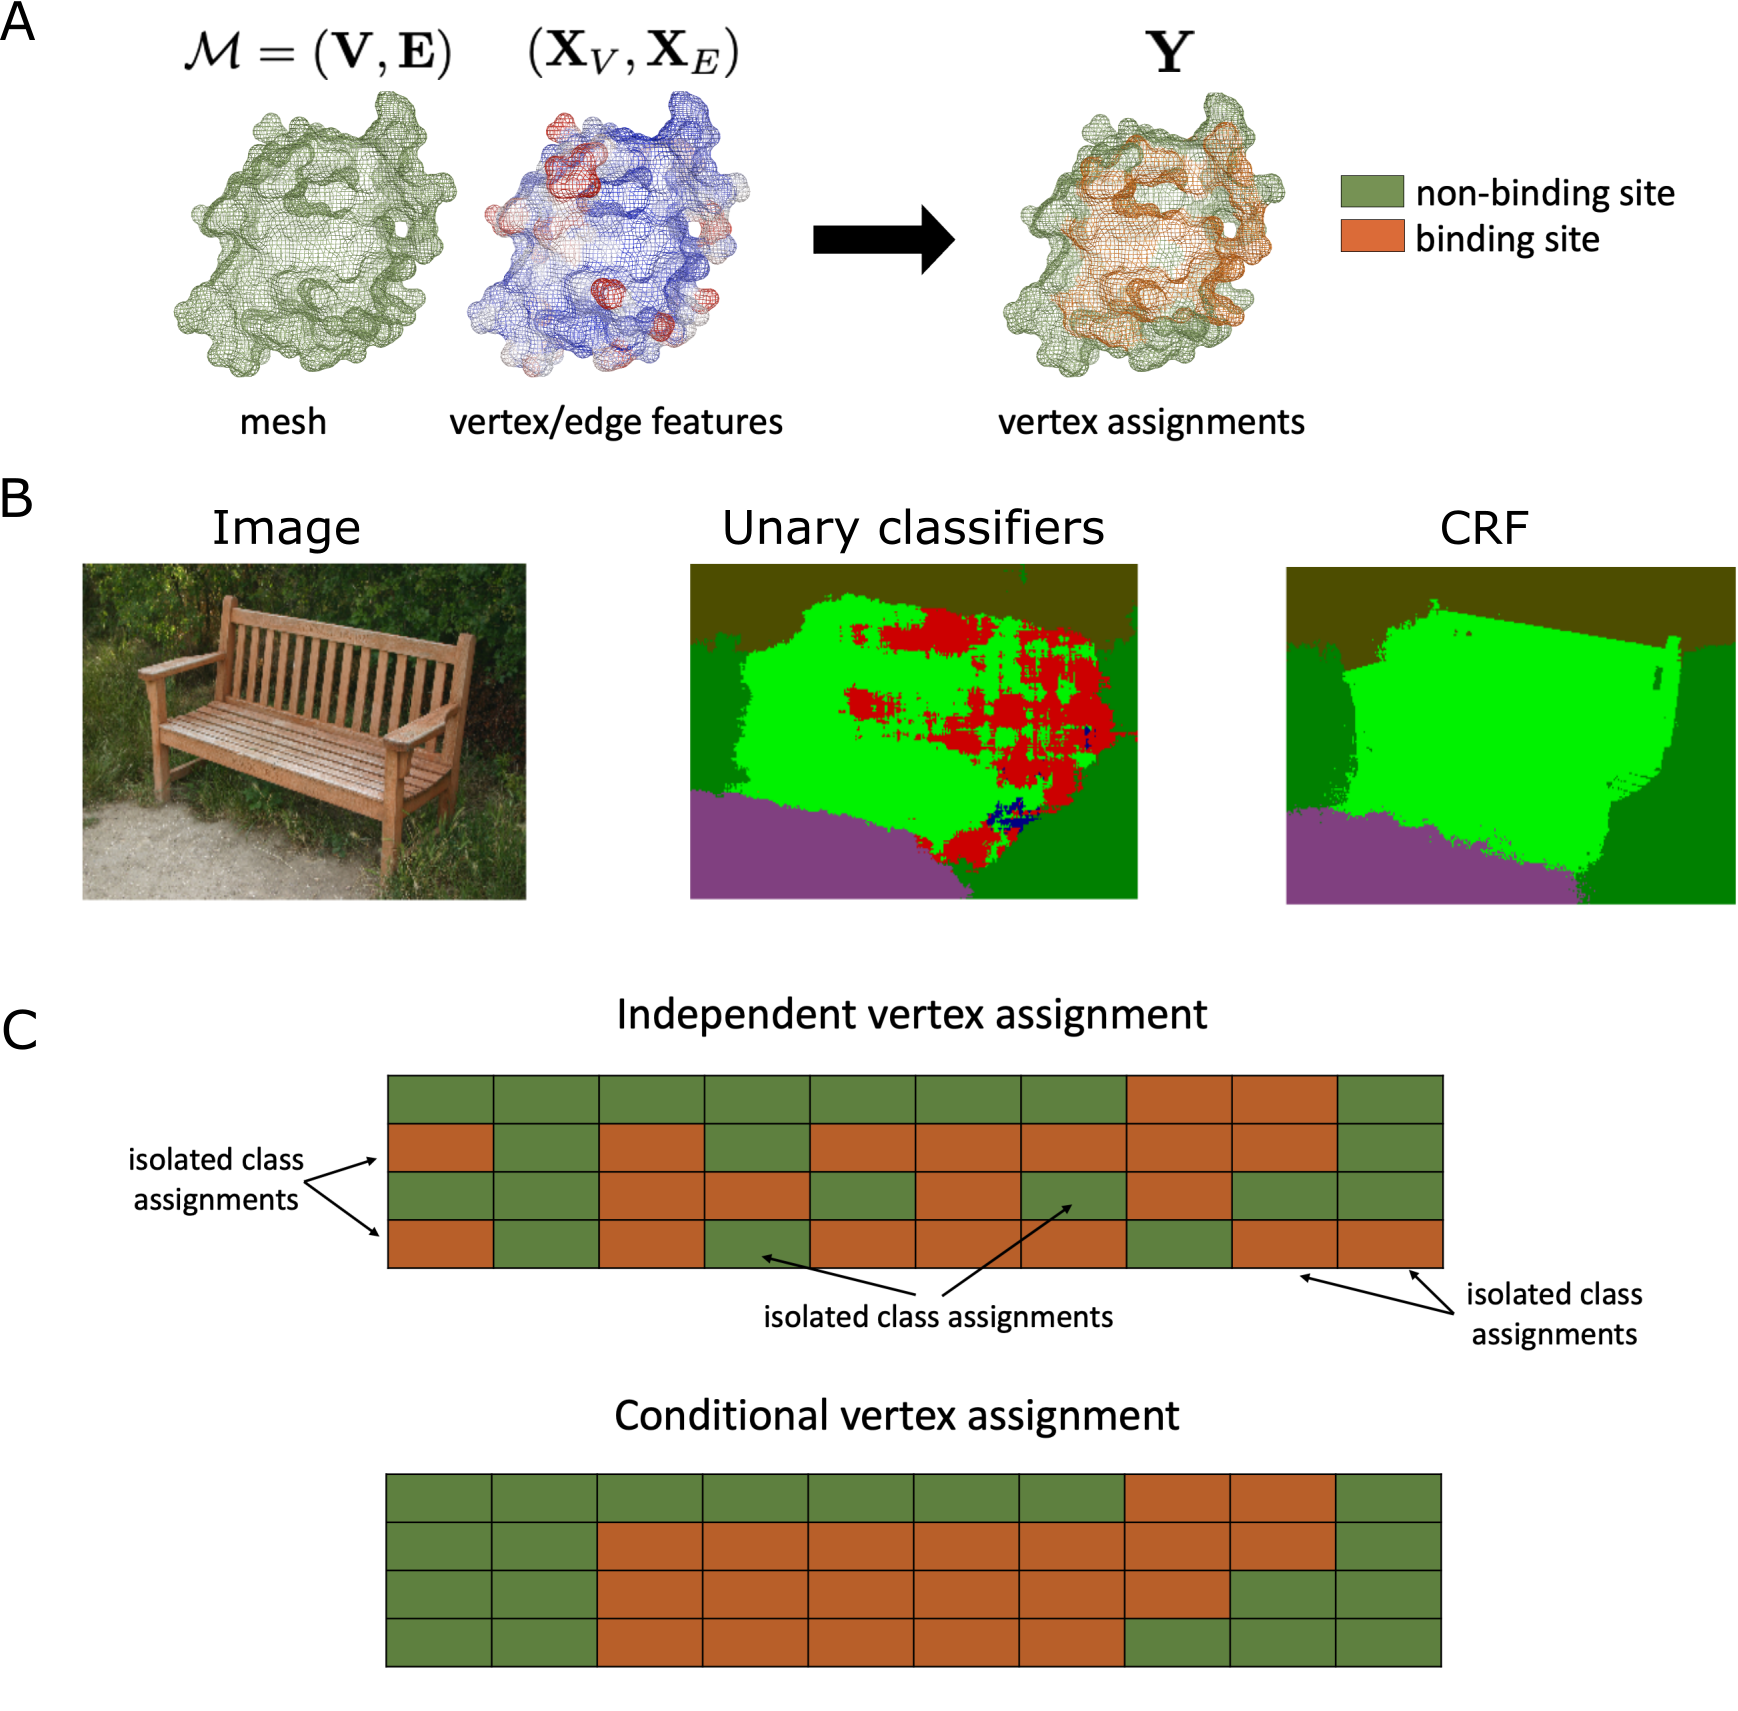
\includegraphics[width=0.8\paperwidth]{crf_figs/crf_concept.png}}
 % archetecture.png: 1149x508 px, 72dpi, 40.53x17.92 cm, bb=0 0 1149 508
        \caption[Geobind schematic, example and conceptual explanation of CRF application scenario]{\textbf{Geobind schematic, example and conceptual explanation of CRF application scenario}
        ({\bf A}) Schematic diagram showing how Geobind predicts binding sites over a protein surface represented as a mesh. ({\bf B}) \citet{krahenbuhl2012efficient} shows how applying a fully connected CRF model results in better image segmentation results compared to 
        just unary classification. ({\bf C}) (above) An exmple independent class assignment in a 2-D grid of cells which is irregular, (below) A smoother classification, which we would 
        expect to get as result of a conditional assignment process.}
        \label{fig:crf_concept} \end{figure} \end{center}

\section{Methods}
We develop a recurrent variational autoencoder to model gene expression dynamics (RVAgene). Here we briefly describe the methods underpinning variational autoencoders, and present the implementation of RVAgene. 

\subsection{Variational inference and variational autoencoders}
In the most general setting of a Bayesian model, we seek to learn the latent variables $\vz$ that best characterize some data $\vx$. Given a generative process that draws latent variables from a prior distribution, $p(\vz)$, and a likelihood of the data observed that is given by $p(\vx|\vz)$, then the posterior probability is given by Bayes rule:
%Our target is to learn about $\vz$ given the observed $\vx$, which is governed simply by the Bayes' rule:
\begin{align*}
 p( \vz | \vx)&= \frac{p(\vx|\vz)p(\vz)}{\int_z p(\vx|\vz)p(\vz) dz}. \numberthis \label{bayes-rule}
\end{align*}
The denominator is often intractable, making it difficult to estimate $p( \vz | \vx)$. Markov Chain Monte Carlo methods provide means to estimate posterior probability distributions. 
An alternative method to estimate hard-to-compute probability distributions is Variational Inference (VI) \citep{Hoffman2013}, which starts from the assumption that the posterior can be approximated by a distribution $q(\vz)$ from the family $\cQ$. VI then amounts to an optimization problem to find the $q^*$ that minimizes the Kullback–Leibler (KL) divergence between the approximation and the true posterior: 
\begin{align*}
 q^*(\vz) &= \textrm{argmin}_{q(\vz)\in\cQ} \textrm{KL}(q(\vz)||p(\vz|\vx)). \numberthis \label{vi-formulation}
\end{align*}

Much recent effort has gone into solving VI problems in different settings \citep{Zhang2019, Ingraham2017, Bouchard-Cote2010}. VI can be framed as solving an optimization problem over function families: neural networks are popular candidates for representing and learning complex functions. VI was incorporated into autoencoders \citep{Kingma2014} to create the architecture of a variational autoencoder (VAE). A VAE consists of an encoder network to approximate $p(\vz|\vx)$ through a function $q_\vx(\vz)$, and a decoder network $p(\vx|\vz)$ (\hyperref[fig:fig2]{Fig. 1A}). Conceptually, the encoder solves an inference problem: approximating the posterior distribution $p(\vz|\vx)$ as some $q^*_\vx(\vz)$, while the decoder solves a reconstruction problem: defining a generative process for $p(\vx|\vz)$, given the latent variables.
The VAE posterior is modeled by a multivariate normal $\cN(\mathbf{\mu},\Sigma)$ of the same dimension as $\vz$. Training then comes down to minimizing two objective functions. For the encoder network, which should learn a ``well distributed'' latent space, minimize the KL divergence: KL$(\cN(\mathbf{\mu},\Sigma) || \cN(0,\vI)) $. For the decoder network, which should reconstruct the inputs $\vx$ from the latent space, minimizing either an $L1$ or $L2$ objective function with respect to $\hat{\vx}$ is appropriate. The use of KL-divergence and an $L2$ objective solves the VI formulation of Eq. \ref{vi-formulation} \citep{Kingma2014}, however, an $L1$ objective may be preferred in practice, e.g. in cases where we want to suppress the effects of outliers on the structure of $\vz$ \citep{botchkarev2018performance}.

% Each input point $\vx_i$ is encoded as a distribution over the latent space $\vz$ given a prior, \tcr{and also project $\vx_i$ to a point $\vz_i$ using the reparametrization trick (\cite{Kingma2014}).} Typically, VAEs typically use a standard normal prior $\cN(0,\vI)$ as the prior distribution over the latent space. The decoder network then takes points from the latent space $\vz$ as input, and generates $\vx$. 


%\begin{center}
%% 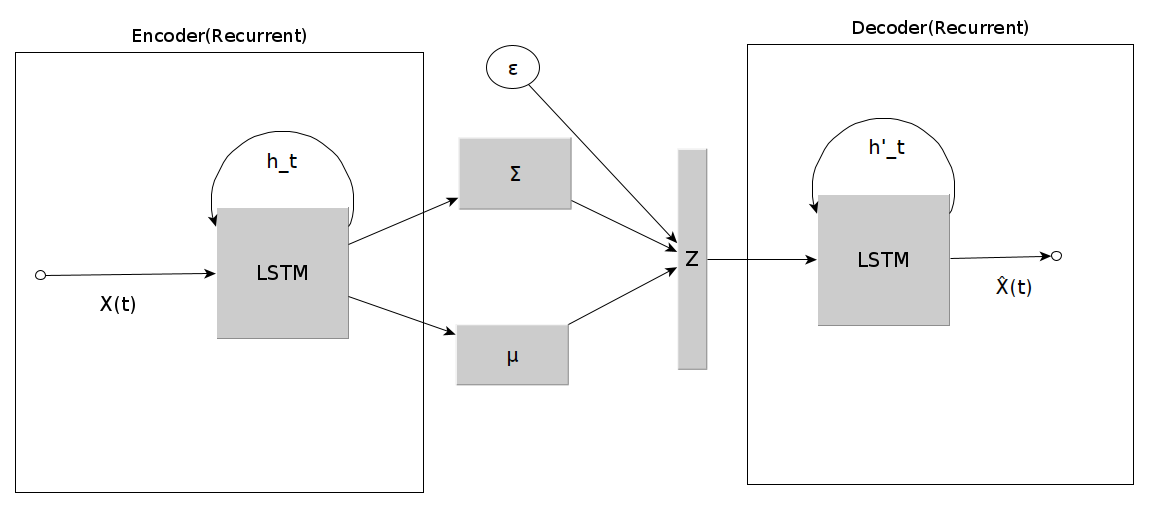
\includegraphics[scale=0.3]{architecture.png} 
%\begin{figure}
%\centering
%  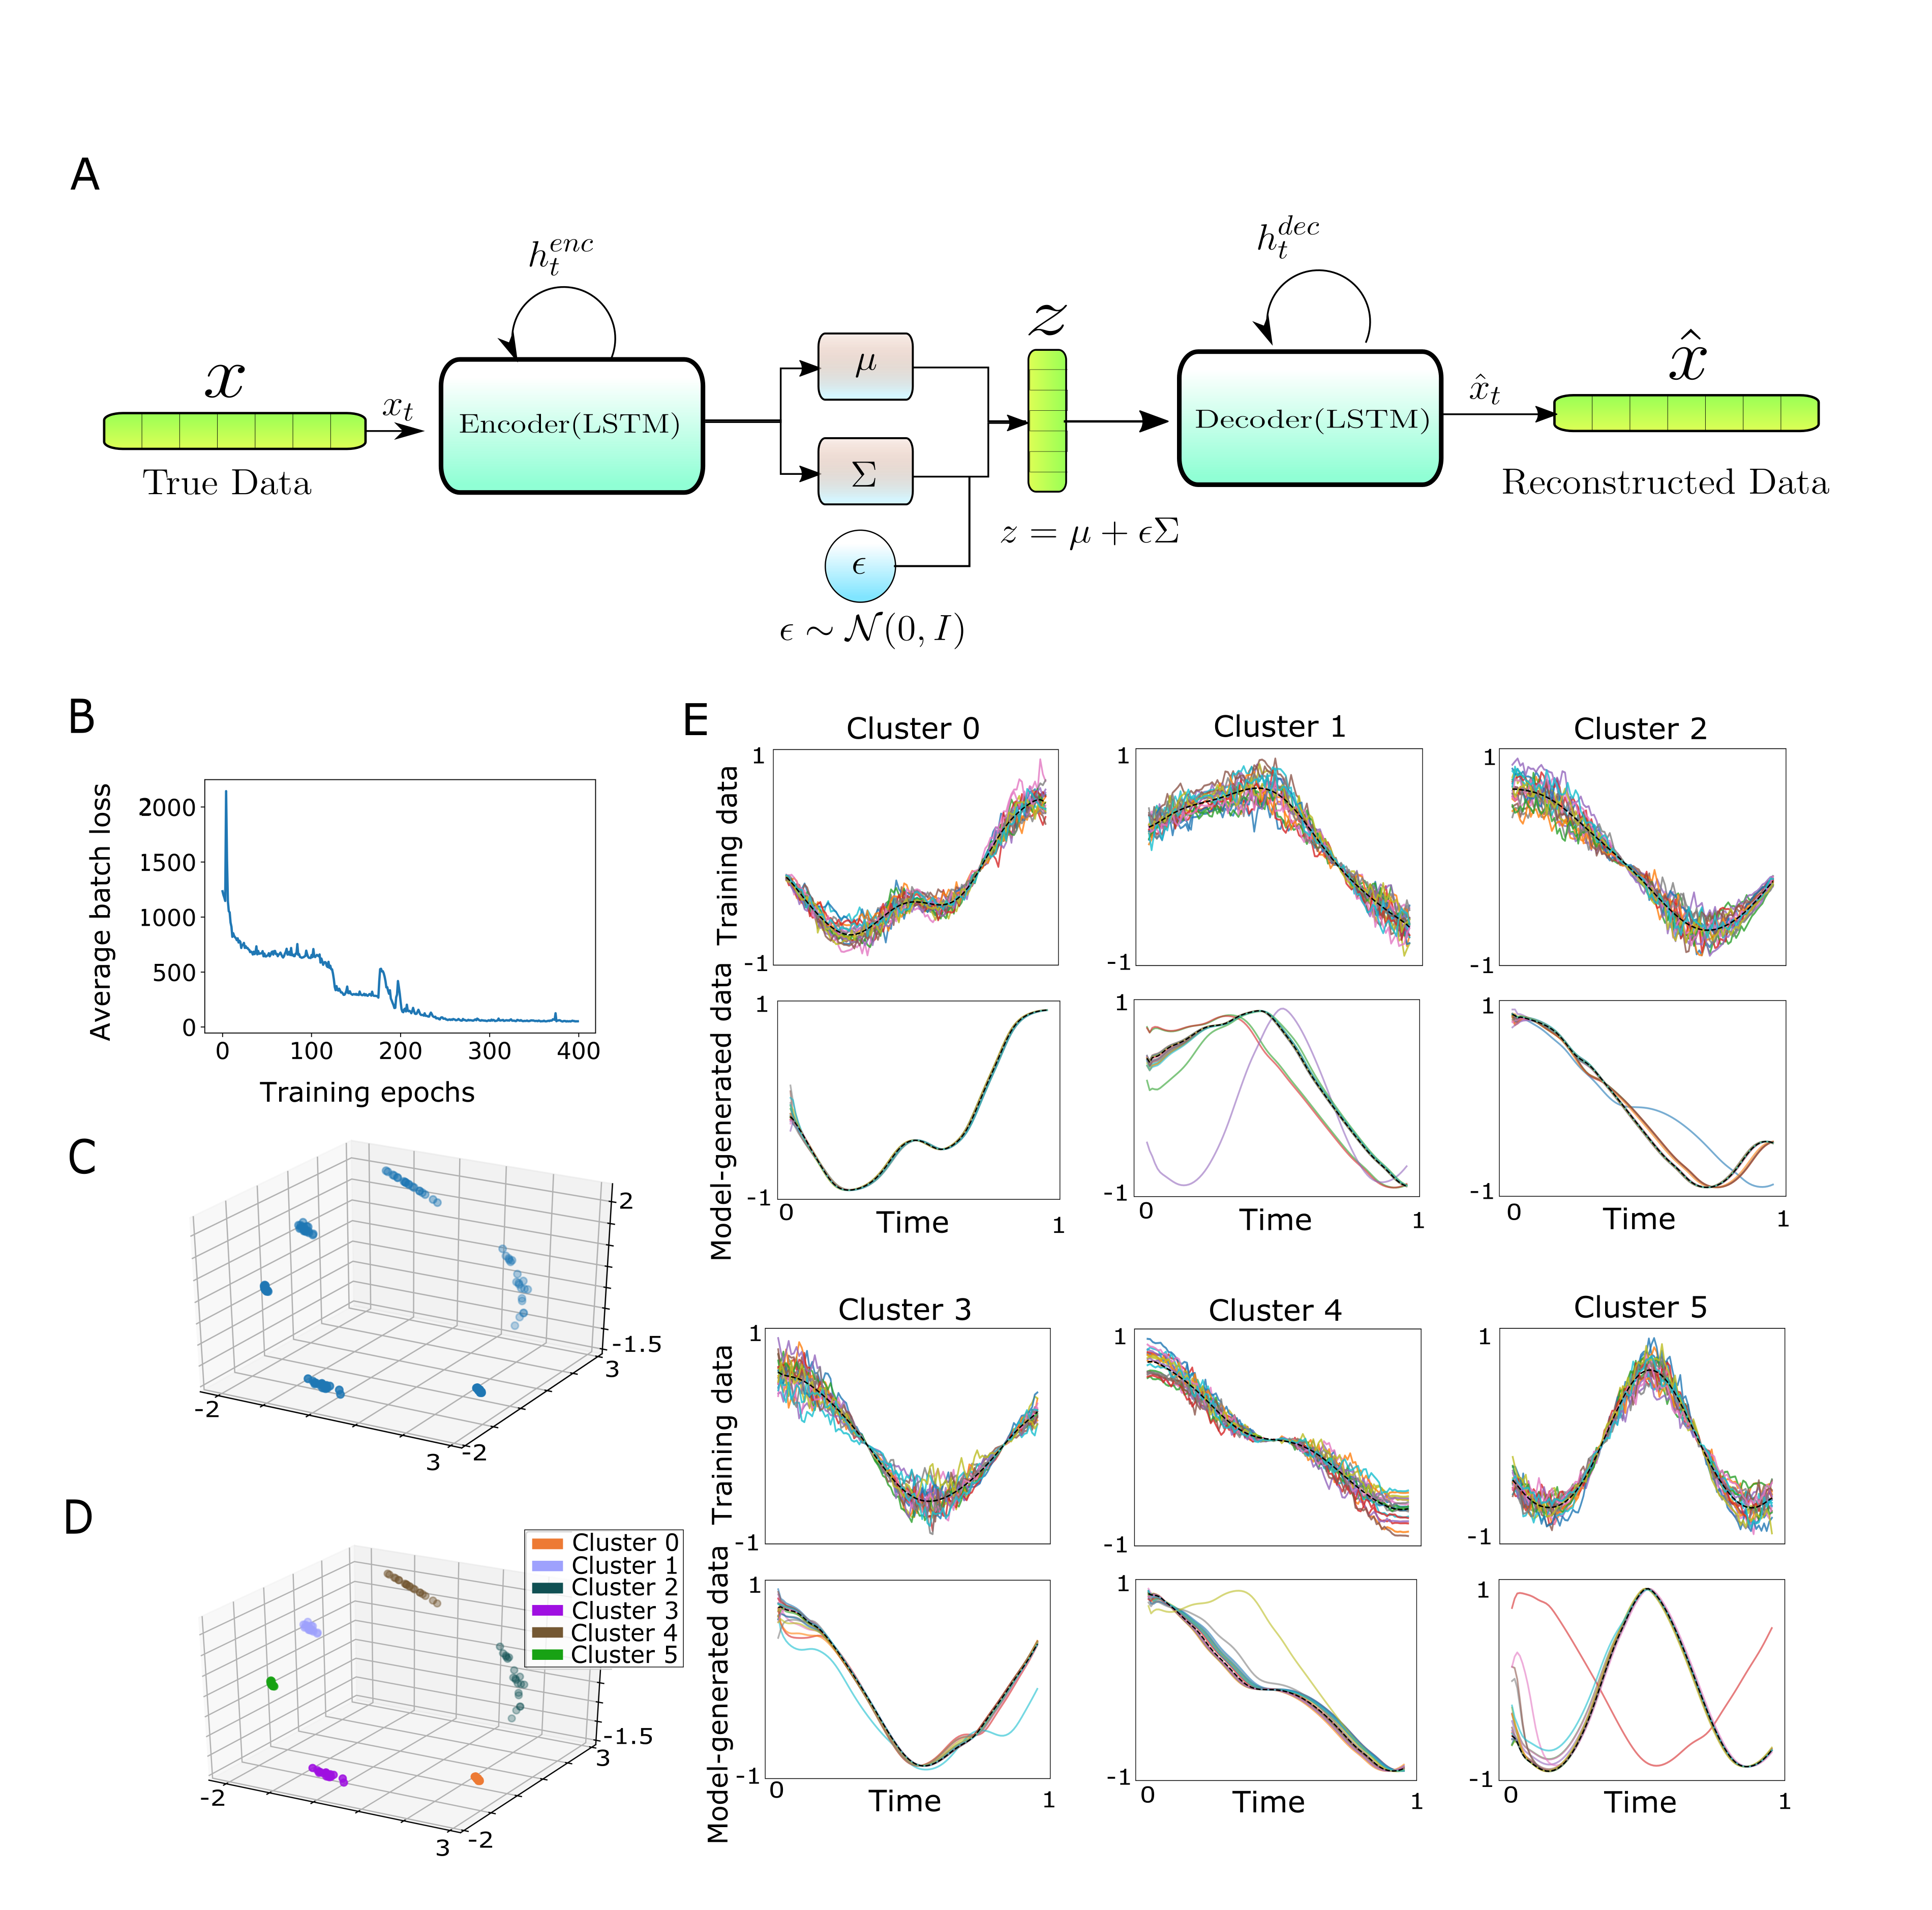
\includegraphics[width=\linewidth]{figures/fig1.png}
% % archetecture.png: 1149x508 px, 72dpi, 40.53x17.92 cm, bb=0 0 1149 508
% \caption{Schematic diagram of RVAgene.}
% \label{fig:scheme}
%\end{figure}
%\end{center}


%% Probably too much detail here, but may want to cite the refs. 
%So far, we haven't specified anything about architecture of the encoder and decoder networks of a VAE, except that they learn certain functions modelling the posterior and likelihood probabilities  of our generative story of the data we are interested in. In general we could make them a fully connected neural network. But, since we are interested in handling sequential (time-series) data, we expect a specific structure of those functions. Intuitively, the $t$-th time point of input sequenece $\vx$ should be causally dependent only on its previous timepoints (upto $t-1$).  Therefore, instead of designing a completely agnostic network (e.g. fully connected layers), we can use a recurrent architecture for the encoder and decoder, which are well established in modelling sequence data (e.g. text data (\cite{Nallapati2016}), time-series data (\cite{Malhotra2015})). This in essence reduces the search space of the model from completely agnostic to a family of recurrent functions.
%\cite{Fabius2015} used this idea and showed how Recurrent Variational Autoencoders can be useful as a unsupervised latent representation learning and generative model for music data.


\subsection{RVAgene: A recurrent variational autoencoder to model gene expression dynamics}
Following the VAE architecture, RVAgene consists of an encoder and a decoder network with a reparameterization step in between. To incorporate the knowledge that we are modeling temporal data, recurrent neural networks offer an ideal architecture to use for both the encoder and the decoder networks. Recurrent and VAE networks have been successfully combined elsewhere, e.g. for textual \citep{Nallapati2016} and time series data \citep{Malhotra2015}.
\par
The architecture of RVAgene is based on \citet{Fabius2015}. An input sequence (i.e. gene) $x \in \vx$, $x = (x_1,x_2,...,x_t,...,x_T)$ is encoded using a recurrent function described by a long short-term memory (LSTM) unit. LSTM units are the state-of-the-art in recurrent architectures, since they are robust against the vanishing gradient problem for longer sequences, unlike other recurrent units (see details in \citet{Hochreiter1997}). We encode $x$ in the following manner:
\begin{align*}
 h_{t+1}^{enc} &= \textrm{LSTM}(W_{enc}^Th_t^{enc} + W_{inp}^T{x_t}+b_{enc}), \numberthis \label{lstm}
\end{align*}
where ($W_{enc}$, $W_{inp}$ and $b_{enc}$) are network weight parameters, and the hidden states $h_t$ represent information shared over timepoints in the LSTM. The dimension of the $h_t$ (and  $W_{enc}$) is given by a hyperparameter (``hidden-size''). The encoded $h_{t+1}$ are used to parametrize the posterior mean and variance from $x$, with mean $\mu_z$ and diagonal covariance $\sigma_z$ as:
%represent this mean and diagonal covariance matrix of the normal distribution an input $x$ is getting encoded to. 

\begin{align*}
 \mu_z &= W_{\mu}^Th_{T+1}^{enc} + b_{\mu} \numberthis \label{mu}\\
  log(\sigma_z) &= W_{\sigma}^Th_{T+1}^{enc} + b_{\sigma}.  \label{sigma}
 \end{align*}
We then use the reparameterization step described in \citet{Kingma2014} to sample $z$ from the distribution:
\begin{align*}
 z = \mu_z + \epsilon\sigma_z, \numberthis 
\end{align*}
where, for known $\epsilon$, backpropagation through the sampling step is possible while training the network.
\par
For the decoder network, the first state $h_1$ is calculated from $z$, and the recurrent formulation follows by reconstructing $x$ as $\hat{x} = (\hat{x}_1,\hat{x}_2,...,\hat{x}_t,...,\hat{x}_T )$, thus:
\begin{align*}
 h_1^{dec} &= \textrm{sigm}(W_{z}^Tz + b_{z})   \\
h_{t+1}^{dec} &= \textrm{LSTM}(W_{dec}^Th_t^{dec} + W_{out}^T{\hat{x}_t}+b_{dec}) \numberthis \label{decoder_lstm} \\
\hat{x}_t &= \textrm{sigm}(W_{out}^Th_t^{dec} + b_{out}), \\
\end{align*}
where $\textrm{sigm}(u) = \frac{1}{1 + e^{-u}}$ is the sigmoid activation function, and ($W_i, b_i$) are the network weight parameters. A schematic diagram of the network is shown in \hyperref[fig:fig2]{Fig. 1A}, which can now be trained using backpropagation, to minimize the objective function: 
\begin{align*}
    \cL(\theta, x) = D_{KL}(\cN(\mathbf{\mu}_z,\Sigma_z)||\cN(\mathbf{0},\vI)) + |x - \hat{x}|, \numberthis \label{lossfunction}
\end{align*}
where $\mathbf{\mu}_z$ and $\Sigma_z = \textrm{diag}(\sigma_z)$ are calculated from $x$ by the encoder.
\par 
To evaluate the accuracy of RVAgene, we need an appropriate error measure. For each gene in the test set, we calculate the $L1$ reconstruction error between generated data $\hat{x}$ and true data $x$, averaged over all time points. We normalize the data to lie in $[0,1]$ to avoid skewing the error by differences in gene expression magnitudes. Thus we define:
\begin{align}
    \textrm{Reconstruction error}(x,\hat{x}) = \frac{1}{T}\sum_{t}| s(\hat{x})_t - s(x)_t |,  & \text{ where } s(x) = \frac{x}{\sum_{t=1}^Tx_t}.
\end{align} 

\subsection{Generating synthetic gene expression time series data}
To test RVAgene, we generate a synthetic time series dataset. Six clusters each containing 20 genes are simulated, where for each cluster $c$, the mean gene expression time series $Y_c = (y_{c1}, y_{c2}, ..., y_{ct})$ was generated using addition or convolution and rescaling of two random sinusoidal functions of the form $k_1\textrm{sin}(k_2t)$, where $k_1,k_2$ are randomly chosen positive integers. Trajectories of cluster members were then generated by sampling from the multivariate normal $\cN(Y_c,\Sigma_c)$. We model $\Sigma_c$ as the positive definite matrix $\alpha Y_cY_c^T$, where $\alpha$ is a scaling factor, we use: $\alpha = 1/|Y_c Y_c^T|$. As defined, $\Sigma_c$ will describe nonzero correlations for all pairs of time points, $(t_i,t_j)$. This is unrealistic, so we set to 0 the entries of $\Sigma_c$ for which column and row indices have a difference of more than some threshold $T$ (we used $T=50$), reflecting the fact that correlations between time points are lost over larger time windows (temporal correlations are local). Note that under this condition, $\Sigma_c$  is no longer necessarily positive definite. The multivariate Gaussian sampler \verb+numpy.random.multivariate_normal()+ implemented in \verb+numpy+ \citep{harris2020array} was used to sample from this augmented $\Sigma_c$.
{After generating a simulated dataset by this process, we also added Gaussian noise, drawn from $\cN(0,0.7)$, to the simulated dataset to produce an additional dataset exhibiting higher levels of noise.}


\section{Results} We compare binding site prediction results between two Geobind networks, one
without a CCRF layer (noCRF) and one with a CCRF layer as its second last layer (CRF). For both
cases we trained and validated the networks on three different datsets. The datasets used are as
follows:\\ \\ \textbf{PDNA-62 :} \citet{ahmad2004analysis} constructed a non-redundant dataset of 62
protein–DNA complexes which has been used in a variety of other studies
\citep{kuznetsov2006transient, wang2006bindn} etc. The protein sequences used were filtered to
ensure a maximum identity of no more than 25\% between any two sequences and the resolution of the
chosen structures was 2.5 A or better. The structures in this dataset contain only helical B-form
DNA.\\ \textbf{PDNA-74 :} We constructed a dataset of 74 single-stranded DNA binding proteins bound
to target ssDNA. We first used the structural database DNAproDB
\citep{sagendorf2017dnaprodb,sagendorf2020dnaprodb} to identify 374 protein-ssDNA complexes based on
structural critera which included ensuring the bound DNA in the structure presented the
single-stranded secondary structure, a minimum length of 4 nucleotides per DNA strand and 40
residues per protein chain, and a minimum of 5 nucleotide-residue interactions (as defined by
DNAproDB). Next, we verified that all proteins identified had known ssDNA binding function based on
annotations from the Gene Ontology knowledgebase \citep{gene2019gene}.  Finally, all protein
sequences were clustered with a 70\% sequence identity threshold using CD-HIT \citep{li2006cd}.
These clusters were then randomly sampled, with up to three samples per cluster, to generate the
final set of 74 protein structures. This sampling method allows us to construct a dataset with
limited amount of sequence redundancy but more conformational sampling than would be possible with a
stricter requirement on sequence redundancy. This is useful in the case of ssDNA where the polymer
is very flexible, but structural data is limited.\\ \textbf{PDNA-224:} a non-redundant dataset of
224 protein-DNA complexes originally constructed by \citet{li2013predna}\\ \begin{center}
        \begin{figure}
                \makebox[\textwidth]{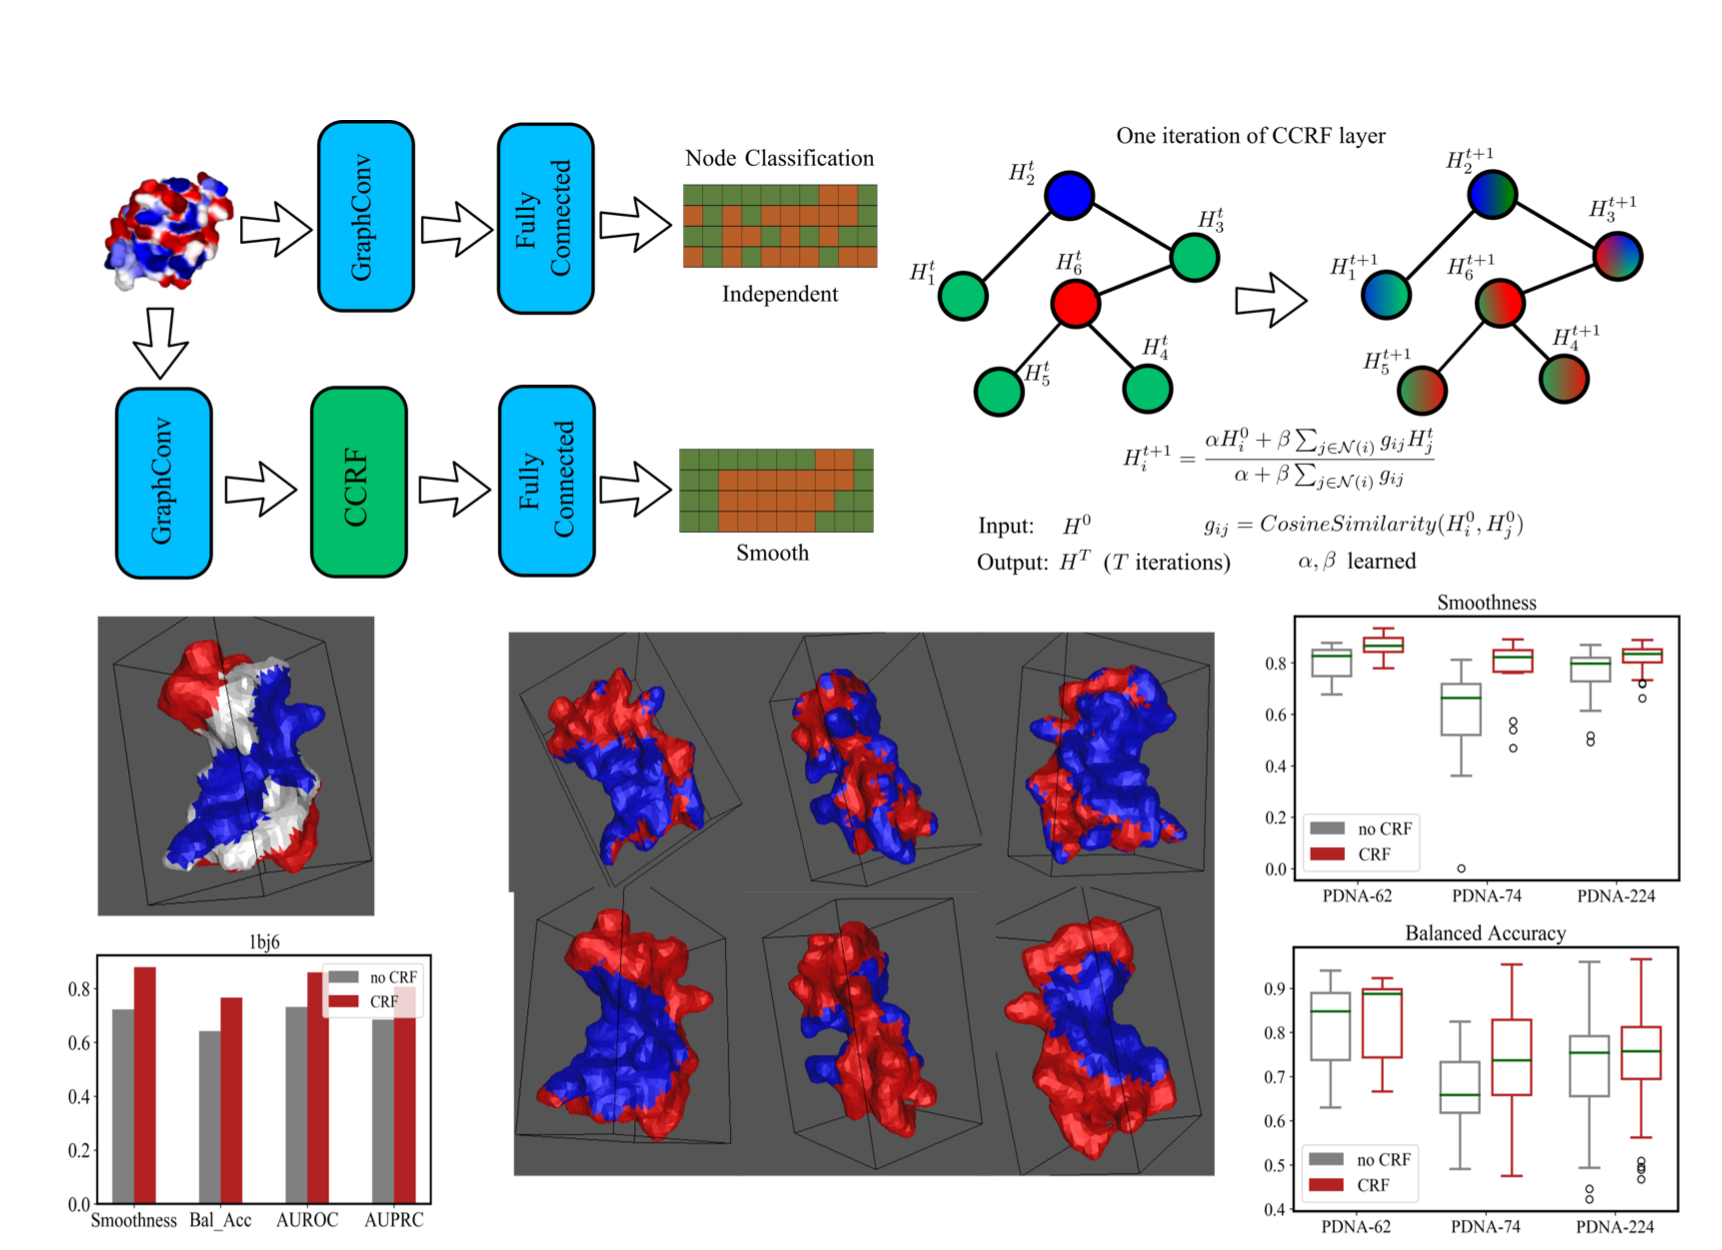
\includegraphics[width=0.8\paperwidth]{crf_figs/demo_crf_fig.png}}
 % archetecture.png: 1149x508 px, 72dpi, 40.53x17.92 cm, bb=0 0 1149 508
        \caption[CCRF for smooth binding site label prediction over protein surface.]{\textbf{CCRF
        for smooth binding site label prediction over protein surface.} ({\bf A}) ({\bf B}) }
        \label{fig:ccrf} \end{figure} \end{center}

Both CRF and noCRF models were trained on the three datasets with a 4:1 training and validation set
        split. \red{\hyperref[fig:ccrf]{Fig. 2.1D}} shows smoothness( eq.
        \ref{final_smoothness_metric}) and Balanced Accuracy  metrics achieved on the validation set
        in each case. We can clearly the smoothness of the predictions have increased significantly.
        It should also be noted that that, median Balanced Acuracy has also increased for all three
        cases. Therefore, we can conclude applying the CCRF layer improves the smoothness of the
        predicted labels over mesh vertices without compromizing in accuracy of prediction. For a
        more visual understanding, \red{\hyperref[fig:ccrf]{Fig. 2.1C}} shows one particular example
        of the effect of using CRF layer against the noCRF model for a protein in the validation set
        for PDNA-74 dataset. The top left panel in \red{\hyperref[fig:ccrf]{Fig. 2.1C}} shows the
        ground truth data. We can clearly see how the CRF model improves smoothness of the
        prediction along with various other classification metrics.



\section{Discussion}
In this chapter we applied mean field Bayesian Variational inference to
design a network layer for PNAbind which results in smoother binding site predictions on protein surfaces. We also designed a smoothness metric appropriate for the task of protein surface segmentation.

In the PNAbind framework, the model predicts whether a protein would bind nucleic acids or not, and segments the protein surface into binding and non-binding regions. However, it does not try to predict binding specificity (i.e. what nucleic acid sequence is preferred) and is only based on protein surface and physicochemical features. We assume there are some commonalities between the proteins binding to, say, ss-DNA (for PDNA-74) and this model implicitly learns those sets of commonalities. 

The PNAbind package has been published as joint work led by Jared Sagendorf, who mentored me in this project, with contributions from Jiawei Hunag, Prof. Xiaojiang Chen and supervised by Prof. Remo Rohs\citep{Sagendorf2024}. In recent years multiple works have been published which compete with PNAbind \citep{gainza2020deciphering, gligorijevic2021structure, yuan2022alphafold2, xia2021graphbind, tubiana2022scannet, krapp2023pesto, li2023geobind, sverrisson2021fast}. But, no deep learning method to predict binding specificity across protein families has been achieved yet.

As a next step, we work towards predicting binding specificity. One of the key challenges in this problem setting is data sparsity. In the next chapter, we present DeepPBS, a model for protein-DNA binding specificity prediction, based on a given co-crystal structural model, which works across protein families.  


%%%%%%%%%%%%%%%%%%%%%%%%%%%%%%%%%%%%%%%%%%%%%%%%%%%%%%%%%%%%%%%%%%%%%%%%%%%%%%%
\chapter{Proposal:  A generalized generative model for binding element design.}
\begin{abstract} 
    Predicting DNA/RNA binding sites on a given protein surface is an important computational task since experminetally determining such information is often expensive and time consuming. Such binding site prediction task can be formulated as a node classification task over a 3D mesh representing the protein surface, with features over the vertices and edges of the mesh representing various geometrical and physicochemical features of the protein structure. At our lab we developed a deep learning based method, which independently classifies mesh vertices as binding and non-binding sites. This often results into irregular binding site predictions over the protein surface. However, intuitively, binding site predictions should be contiguous and not patchy i.e. as ``smooth" as possible while being correct. In this chapter, we describe what such kind of ``smoothness" entails and we improve upon the original architecture by desigining a network layer based on a  probabilistic Continuous Conditional Random Field (CCRF) model, which increases smoothness of binding site prediction while improving prediction accuracy of the model. This network layer was incorporated into the original model and published as Geobind package (\red{Sagendorf et. al}).
\end{abstract}

\section{Introduction} 

Designing binding elements for target regions in protein residues or complexes is a hard
computational problem  which has huge impact in biotechnology and pharmaceutical ventures.
This constitutes of drug design and nucleic acid sequence/position weight matrix (PWM)
design. The processes generally employed in solving these kind of problems are traditionally virtual and
experimental screening of large amount of candidate binding elements. These processes are extremely
computationally/experimentally intensive and costly. 
\par
Recently, generative machine learning models have
been used to make significant advances in such tasks. The key models generative models that are most
used are mainly of two kind: Variational Autoencoders (VAE) \citep{Kingma2014} and its many
variations \citep{higgins2016beta, sohn2015learning,dilokthanakul2016deep}; Generative Adversarial
Networks \citep{goodfellow2014generative} and variations \citep{wang2018high,zhu2017unpaired}.
\citet{gomez2018automatic} first proposed a variational autoencoder model for drug molecule design.
Similar to RVAgene \red{(cite)} this method encodes training drug molecules represented as SMILES
\citep{weininger1988smiles} string in a regularized latent space which then can be sampled and
decoded to generate new candidate molecules. They also train an additional network to optimize the
generative process based on given chemical properties. This initial model sparked a flurry of folow up 
works mainly addressing various aspects of the problem: e.g. enforcing constraints on the generative process 
such that the generated molecules are chemically valid \citet{kusner2017grammar}, increasing diversity of the generated
molecules, conditional generation etc. 

\section{Proposed Method} 
In chapter 1, we learned a generative model of gene expression time
series data using a VAE framework, where we learned a regularized latent space representation of latent
variables $z$ by reconstructing the data $x$ through an encoder-decoder architecture. We can start
thinking about the binding element design problem in the same manner.

Let's define $x_p$ as input binding site information. We want to predict a binding element $x_e$
given $x_p$. To achieve this task, we again formulate a generative story: $x_e$ is generated from
latent variables $z$, which can be modeled by a decoder/generator network which models the
distribution $P(x_e|z)$. And we can employ an encoder network modeling $P(z|x_p)$ to achieve the
latent information $z$ from the input $x_e$.

Now, to formally achieve the prediction task, we start with writing out the conditional distribution,
$P(x_e, z|x_p)$ which we would like to maximize and predicts the argument $x_e$ and $z$ that maximizes it.

\begin{align*}
        P(x_e,z|x_p) = P(x_e|z,x_p)P(z|x_p) \;\;\; \text{using Bayes' rule}\numberthis
\end{align*}
Here, we assume a hierarchical Bayesian setting where given the latent variable $z$, $x_e$ is
generated independent of $x_p$ i.e. $P(x_e|z,x_p) = P(x_e|z)$. Now we can write the following,
\begin{align*}
P(x_e,z|x_p) &= P(x_e|z)P(z|x_p) \numberthis \\
\end{align*}
Now, we can model the posterior of $z$, $P(z | x_p)$ as a Gaussian $N(z_{\mu}, z_{\Sigma})$. This
can be modeled by outputing the parameters $z_{\mu}, z_{\Sigma}$ from an encoder network $E(x_p)$.
A value of $z$ can be sampled from this distribution now using the reparamtrization trick described
in \citet{Kingma2014}, similar to as described in Chapter 1 for RVAgene. This process along with a
KL loss with a prior on $z$ $p(z) = N(0,\bI)$ ensures a regularized latent space which is important
for generating meaningful data. Therefore,
\begin{align*}
        z_{\mu}, z_{\Sigma} &= E(x_p) \numberthis \\
        \hat{z} &= z_{\mu} + \epsilon \cdot z_{\Sigma} \;\; where \;\; \epsilon \sim N(0,\bI) \numberthis \\
        \hat{x}_e &= argmax_{x_e}p(x_e | \hat{z}) = G(\hat{z}) \;\; \numberthis \label{final_prediction_architecture} 
\end{align*}
%\implies \text{prediction } \hat{x}_e, \hat{z} &= argmax_{x_e,z} P(x_e,z|x_p) \numberthis \\
%&= argmax_{x_e,z} P(x_e|z)P(z|x_p)  \\
%\implies  \hat{z} = argmax_{z} P(z|x_p); & \;\;\;\;\hat{x}_e = argmax_{x_e} P(x_e | \hat{z}) \numberthis \\
%\implies \hat{z} = E(x_p); & \;\;\;\; \hat{x}_e = G(\hat{z}) \numberthis
The functions $E(x_p)$ and $G(\hat{z})$ in \ref{final_prediction_architecture} represent the
encoder and generator functions respectively both of which are parametrized by neural networks. 

Now, the encoder-generator framework described above is suitable for prediction, however it's
difficult to train it in a straight forward manner. For RVAgene \red{(cite)} we were able to use
reconstruction based method to train because the input of encoder and output of decoder was the same.
Here, they are different. This constitutes a proper scenario to employ an adversarial training
scheme as employed by GANs \citep{goodfellow2014generative}.

Given a training dataset $X$ consisting of $n$ datapoints, where $X_i = (x_p^i, x_e^i) \;\; i \in
\{0,..., n-1\}$, we now describe
how to train the generative model described in \ref{final_prediction_architecture}. We assign a
label variable $y = 1$ for all datatpoints in the training data $X$. Now, assume we have some
datapairs $F = (x_p^i, \hat{x}_e^i) \;\; i \in \{0,..., m-1\}$ generated by the encoder-generator
system given $x_p^i$s as input. We assign these datapoints a label $y = 0$. Now, we can train a
neural network $D$ discriminating between the datasets X and F i.e. the discriminator $D$ is
predicting $P(y = 1 | x_p, x_e)$. It is clear that the better the enocder-generator system is in
predicting binding element given a protein surface, the harder the job of the discriminator becomes.
We take advantage of this fact and teach the encoder-generator network to try to best the
discriminator and vice versa. The two networks play the following minimax game:
\begin{align*}
        min_{G,E}max_{D} V(D, E, G) &= \bE_{x_p, x_e \sim P_X}\bigg{[}log D(x_p, x_e)\bigg{]} + \bE_{x_p \sim
        P_{x_p}}\bigg{[}log(1 - D(x_p,G(\hat{z}))) + KL(N(z_{\mu}, z_{\Sigma}) || N(0, \bI))\bigg{]} \numberthis \label{gan_game}\\
        &where \; \hat{z} = z_{\mu} + \epsilon z_{\Sigma} \;\; where \; \epsilon \sim N(0,\bI)\; and \;
        z_{\mu}, z_{\sigma} = E(x_p)
\end{align*}
In eq. \ref{gan_game} above $P_X$ represents the full training data distribution and $P_{x_p}$
represents the marginal distribution of binding sites in the training data. 

If we call the generated distribution of $x_p, \hat{x}_e$ as $p_g$, as described and proven in
\citet{goodfellow2014generative} this adversarial game 
eventually results into the generated data distribution becoming same as the training data
distribution $P_x$, which
happens at the point when both the $(E, G)$ and $D$ network cannot improve anymore.

\section{Discussion}
In this chapter we described our proposal for designing a generative model for design binding
elements given binding site information on protein surface. The proposed model is a variation over the VAE
framework \citep{Kingma2014} for unsupervised representation learning. However, it should be noted,
that the architecture described here is not final can change after further experimentation.

Next, we need to shade a little bit of light on the datasets that can be used to train such a model.
Primary source for all our data will be the protein data bank \citep{berman2000protein}. For PWM
generation, the databases JASPAR \citep{fornes2020jaspar} and TRANSFAC \citep{wingender2008transfac}
are good candidates for sources of protein-motif data. However, it should
be noted that, for nucleic acid PWM generation, although the prediction task is PWM generation, the
training data does not need PWM information. Computationally sequences and PWMs are equevalent. the model
sees both sequences and PWMs as a vector of dimension $L \times 4$ ($L$ is length of the
sequence/PWM). Only difference, the vectors are one-hot for sequence and can have fractional values
for PWMs i.e PWMs are soft sequences only. Therefore, it is possible to train the model with
sequence data directly provided the data is rich enough and PWM information is not needed in the
training set. 

Another point that should be discussed is concerning the architecture of Encoder and Generator
networks. The encoder network, although performing the same task for both the drug molecule
generation setting and PWM generation setting, may need to have different architectures. This may be necessary because binding sites for drug molecules are much smaller tha
nucleic acid binding sites (which therefore, can also be discontinuous). This would lead to a point
cloud representation being more favourable compared to mesh representation for PWM generation task.
The generator network will have different architectures based upon the way the binding element
generated is represented as discussed earlier in this chapter.

We hope this project becomes a success and we can present it as a powerful computational tool to the
Computational Biology and Bioinformatics community.

%%%%%%%%%%%%%%%%%%%%%%%%%%%%%%%%%%%%%%%%%%%%%%%%%%%%%%%%%%%%%%%%%%%%%%%%%%%%%%%%%%%%%%%%%%%%%%%%%%%%%%%%%%%%%%%%%%%%%%%%%%%%%%%%%
\chapter{Conclusion and future work}
%\Chapter[Conclusion]{Conclusion}

I joined the QCB department at USC as a PhD student in August 2019. The rigorous curriculum of the CBB PhD program helped me shape my scientific vision and research skills. Soon, the COVID19 pandemic changed everything about our life and uncertainty covered the world. Thankfully, due to wise and loving care of the department, my adviser Prof. Remo Rohs and other members of the QCB department, I was able to continue my work through the difficult times. Prof. Adam MacLean orked hard to help me finish the RVAgene project and get it published \citep{Mitra2021}. The pandemic affected scientific travel oppportunities severely, during those intial years of my PhD. However, later on I was fortunate to be able to travel to numerous high quality conferences and present my work there. I am thankful to my advisor Prof. Remo Rohs for providing me with these opportunities. In fact, meeting Prof. Ada Yonath (Nobel prize, 2009, for solving the structure of ribosome \citep{schluenzen2000structure, harms2001high}) has been one of the most memorable experience of my life. I am also thankful to prof. Yonath for supporting us on the RNAscape project. 


Overall, it has been a fascinating experience to work in the intersection of artificial intelligence and structural biology during these past years. In 2021, we witnessed a more than half a century old problem, protein folding, being almost solved by AlphaFold2 \citep{Jumper2021}, as I was working on my project of modeling protein-DNA binding specificity based on structures. Efforts were immediately underway, to attempt to predict structures of higher order complexes of biomolecules \citep{evans2021protein,baek2024na}, and recently took a big step forward through AlphaFold3 \citep{Abramson2024}. However, these complex structure prediction methods, thus far, are not yet able to model binding specificity. This puts our model, DeepPBS \citep{Mitra2024}, which can look at a predicted or designed complex, and pedict binding specificity in a uniquely synergistic position. In my view, combination of structure prediction and specificity prediction methods is the future of predicting/desgining biologically meaningful complexes. In fact, a fresh direction of thinking about this problem is joint modeling of structure and specificity. However, this is still quite ambitious as data sparsity poses a big challenge, especially for complexes involving nucleic acids. 

Alongside my work on protein-DNA, concurrent events, and my advisor's encouragement inspired me to explore the field of RNA biology, which led to the projects, RNAscape and RNAproDB. As of now, the field of RNA structures is also being shaped by artificial intelligence methods \citep{he2024ribonanza}. However, an AlphaFold level breakthrough is still out of reach \citep{schneider2023will}. Recent works have shown progress in protein structure targeted RNA structure design \citep{nori2024rnaflow} and prediction of protein-RNA binding energy \citep{han2024copra}. Although promising, a lot of it is still quite preliminary and/or lacks biological validation. A DeepPBS like model for RNA binding specifcity prediction is also non-existent (although there has been some progress \citep{Lam2019}). It has also been known for a while that solvent molecules have an effect on protein-nucleic acid recognition \citep{Otwinowski1988}. However, the extent of this phenomenon has not been quantified.

Structure, function and localization of non-coding RNA is also something that remains to be studied and modelled. 70-90\% mammalian genome get transcribed into RNA, but only 1\% of it get translated. Rest are known as ncRNA (non coding RNA). lncRNAs are defined by their size range of 200 bases to 10kilobases. For a long time lncRNAs were regarded as only transcriptional noise. But, recently, it has been shown that they perform important important regulatory functions. Variations in lncRNA expression has been shown to be significantly correlated with certain disease traits \citep{wapinski2011long} and they are tissue-specific \citep{seifuddin2020lncrnakb}. 
\citet{al2019long} shows that lncRNA expression actually better explains certain cancer
classification data compared to mRNA expression. Recent work on population-scale tissue transcriptomics \citep{de2021population} discovers high tissue specific regulation of lncRNA. They also identify 800 lncRNA-trait relationships which are not explained by protein coding genes. Hence, there is a growing interest in developing computational methods addressing various kinds of biological problems in lncRNAome. \citet{alam2020deep} discusses Deep Learning methods recently being developed for
such tasks. Some of these works include, lncRNA-protein interaction prediction
\citep{pan2016ipminer, zhao2018bipartite, yi2018deep, zhan2019bgfe, peng2019rpiter}, lncRNA  identification \citep{baek2018lncrnanet,yang2018lncadeep, tripathi2016deeplnc},
learning regulatory information \citep{alam2019deepcnpp, alam2019deepel}, predicting subcellular localization of lncRNAs \citep{gudenas2018prediction},    lncRNA-miRNA interaction prediction \citep{huang2019predicting}, lncRNA-disease association prediction \citep{hu2019deep, xuan2019dual, al2019long, xuan2019graph} etc. All these tools might improve in future through incorporation of structural and specificity information, as structure and specifcity prediction methods evolve over time.

With the improvements in structure prediction and design, there is an increasing need of high quality analysis tools for the biologists to be able to study, visualize and explore these structures. In later part of my PhD, we built an updated DNAproDB, RNAscape \citep{Mitra2024rnascape} and RNAproDB to address this need. These tools are 
designed to 

Data driven modeling, especially probabilistic machine learning, has been the main theme of my
research. I am extremely grateful for being able to work with so many great minds here at USC and I
hope I can make more meaningful contributions to the collective gathering of human knowledge in
future. Thus I conclude my dissertation proposal.

%%%%%%%%%%%%%%%%%%%%%%%%%%%%%%%%%%%%%%%%%%%%%%%%%%%%%%%%%%%%%%%%%%%%%%%%%%%%%%%%%%%%%%%%%%%%%%%%%%%%%%%%%%
% Conclusion and ongoing work
%\chapter{Conclusion and ongoing work}
\label{cha:conclusion}

\Blindtext[2]


% Using single-space for reference list.
\begin{singlespace}
% Bibliography
%\phantomsection
%\addcontentsline{toc}{chapter}{References}%
%\markboth{References}{References}%
% If you use BibLaTeX
%\printbibliography[title=References]
% If you use BibTeX
\bibliography{library}
\bibliographystyle{agsm}
\end{singlespace}

\subsection*{Supplementary figures}
\label{supp}

\renewcommand{\thefigure}{S\arabic{figure}}
\setcounter{figure}{0}
\begin{center}
\begin{figure}[H]
  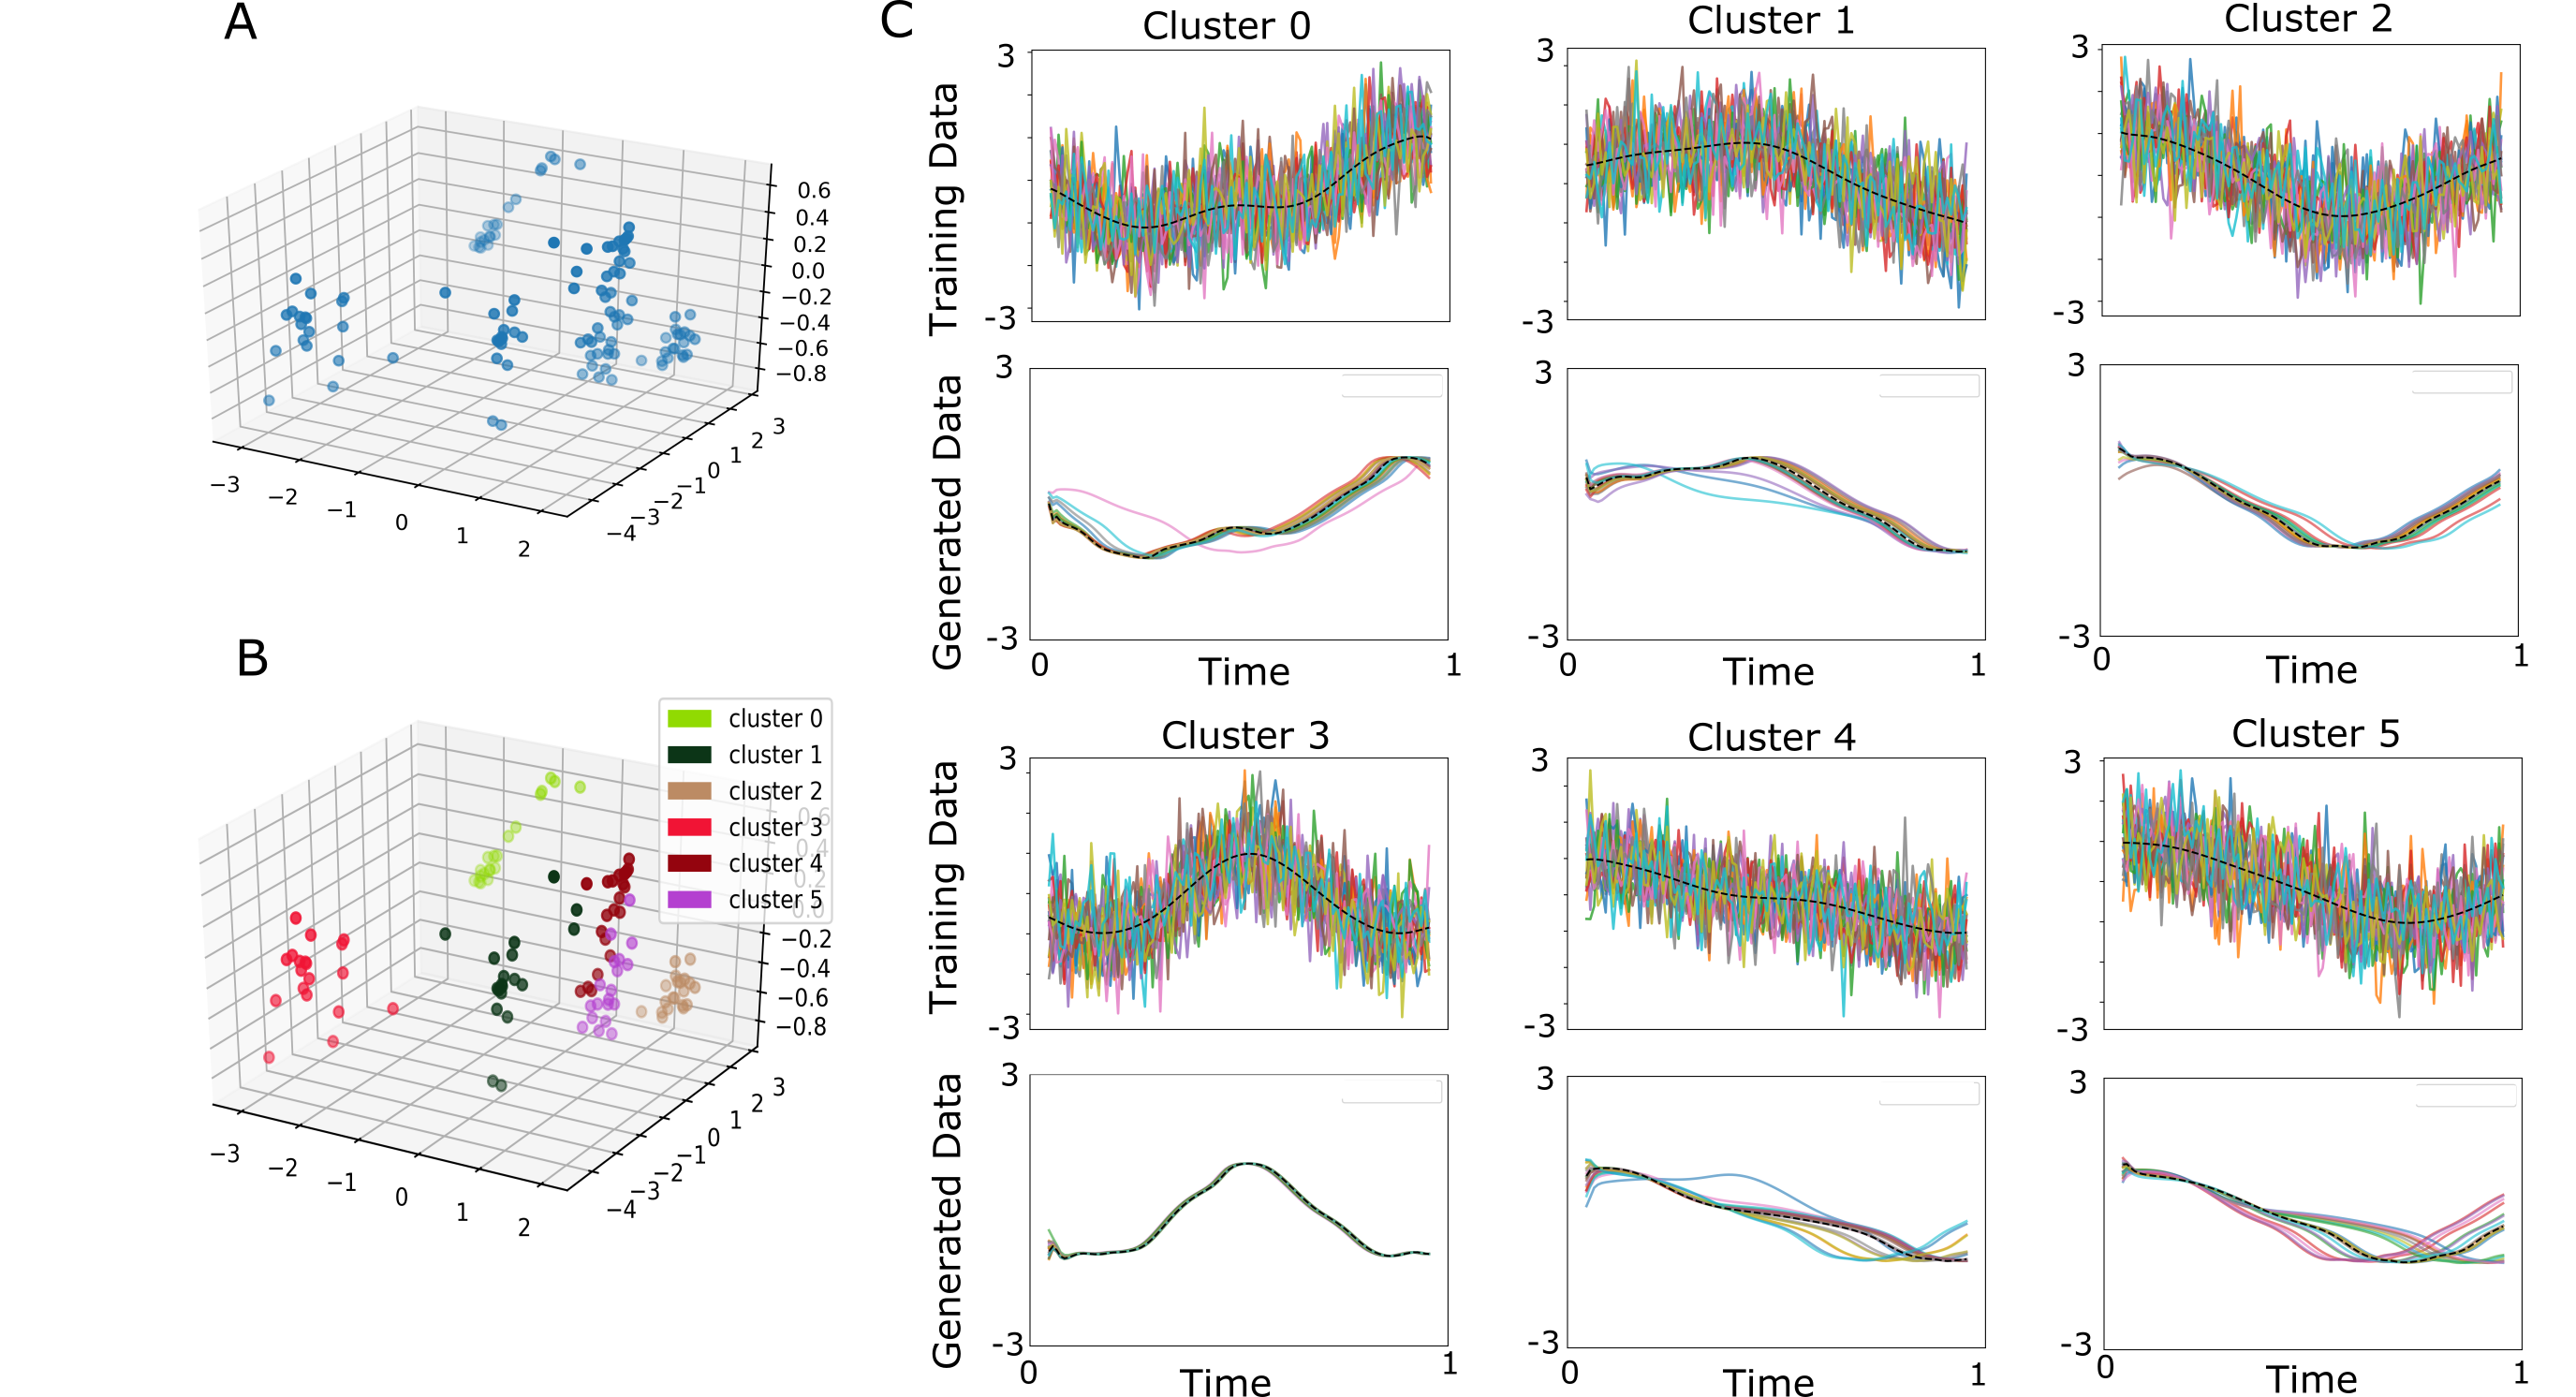
\includegraphics[width=\linewidth]{./figures/noisy_sim.png}
 % archetecture.png: 1149x508 px, 72dpi, 40.53x17.92 cm, bb=0 0 1149 508
    \caption[Demonstration of RVAgene working principle on simulated data with high noise.]{\textbf{Demonstration of RVAgene working principle on simulated data with high noise.} Gaussian noise drawn from $\cN(0,0.7)$ was added to the simulated data to produce a dataset with heavy noise. RVAgene learns the latent space shown in ({\bf A}). ({\bf B}) shows 6 clusters learned by k-means on the learned latent space. ({\bf C}) shows original training data and model generated data from random points in the latent space sampled from $\cN(\mu,0.4\bI)$ around each cluster mean $\mu$ for each of the 6 clusters detected by k-means.}
  \label{fig:figS1}
\end{figure}
\end{center}
\newpage

\begin{center}
\begin{figure}[H]
  \includegraphics[width=\linewidth]{./figures/sl_ESC_r.png}
 % archetecture.png: 1149x508 px, 72dpi, 40.53x17.92 cm, bb=0 0 1149 508
    \caption[Characterization of gene dynamics by linear fit using Pearson correlation coefficient for 5 sample genes in the ESC differentiation dataset]{Characterization of gene dynamics by linear fit using Pearson correlation coefficient for 5 sample genes in the ESC differentiation dataset  \citep{Klein2015}. Blue lines represents original data and orange lines represents linear fits. The Pearson correlation coefficient $r$ is given for each plot.}
  \label{fig:figS2}
\end{figure}
\end{center}
\newpage

\begin{center}
\centering
\begin{figure}[H]
  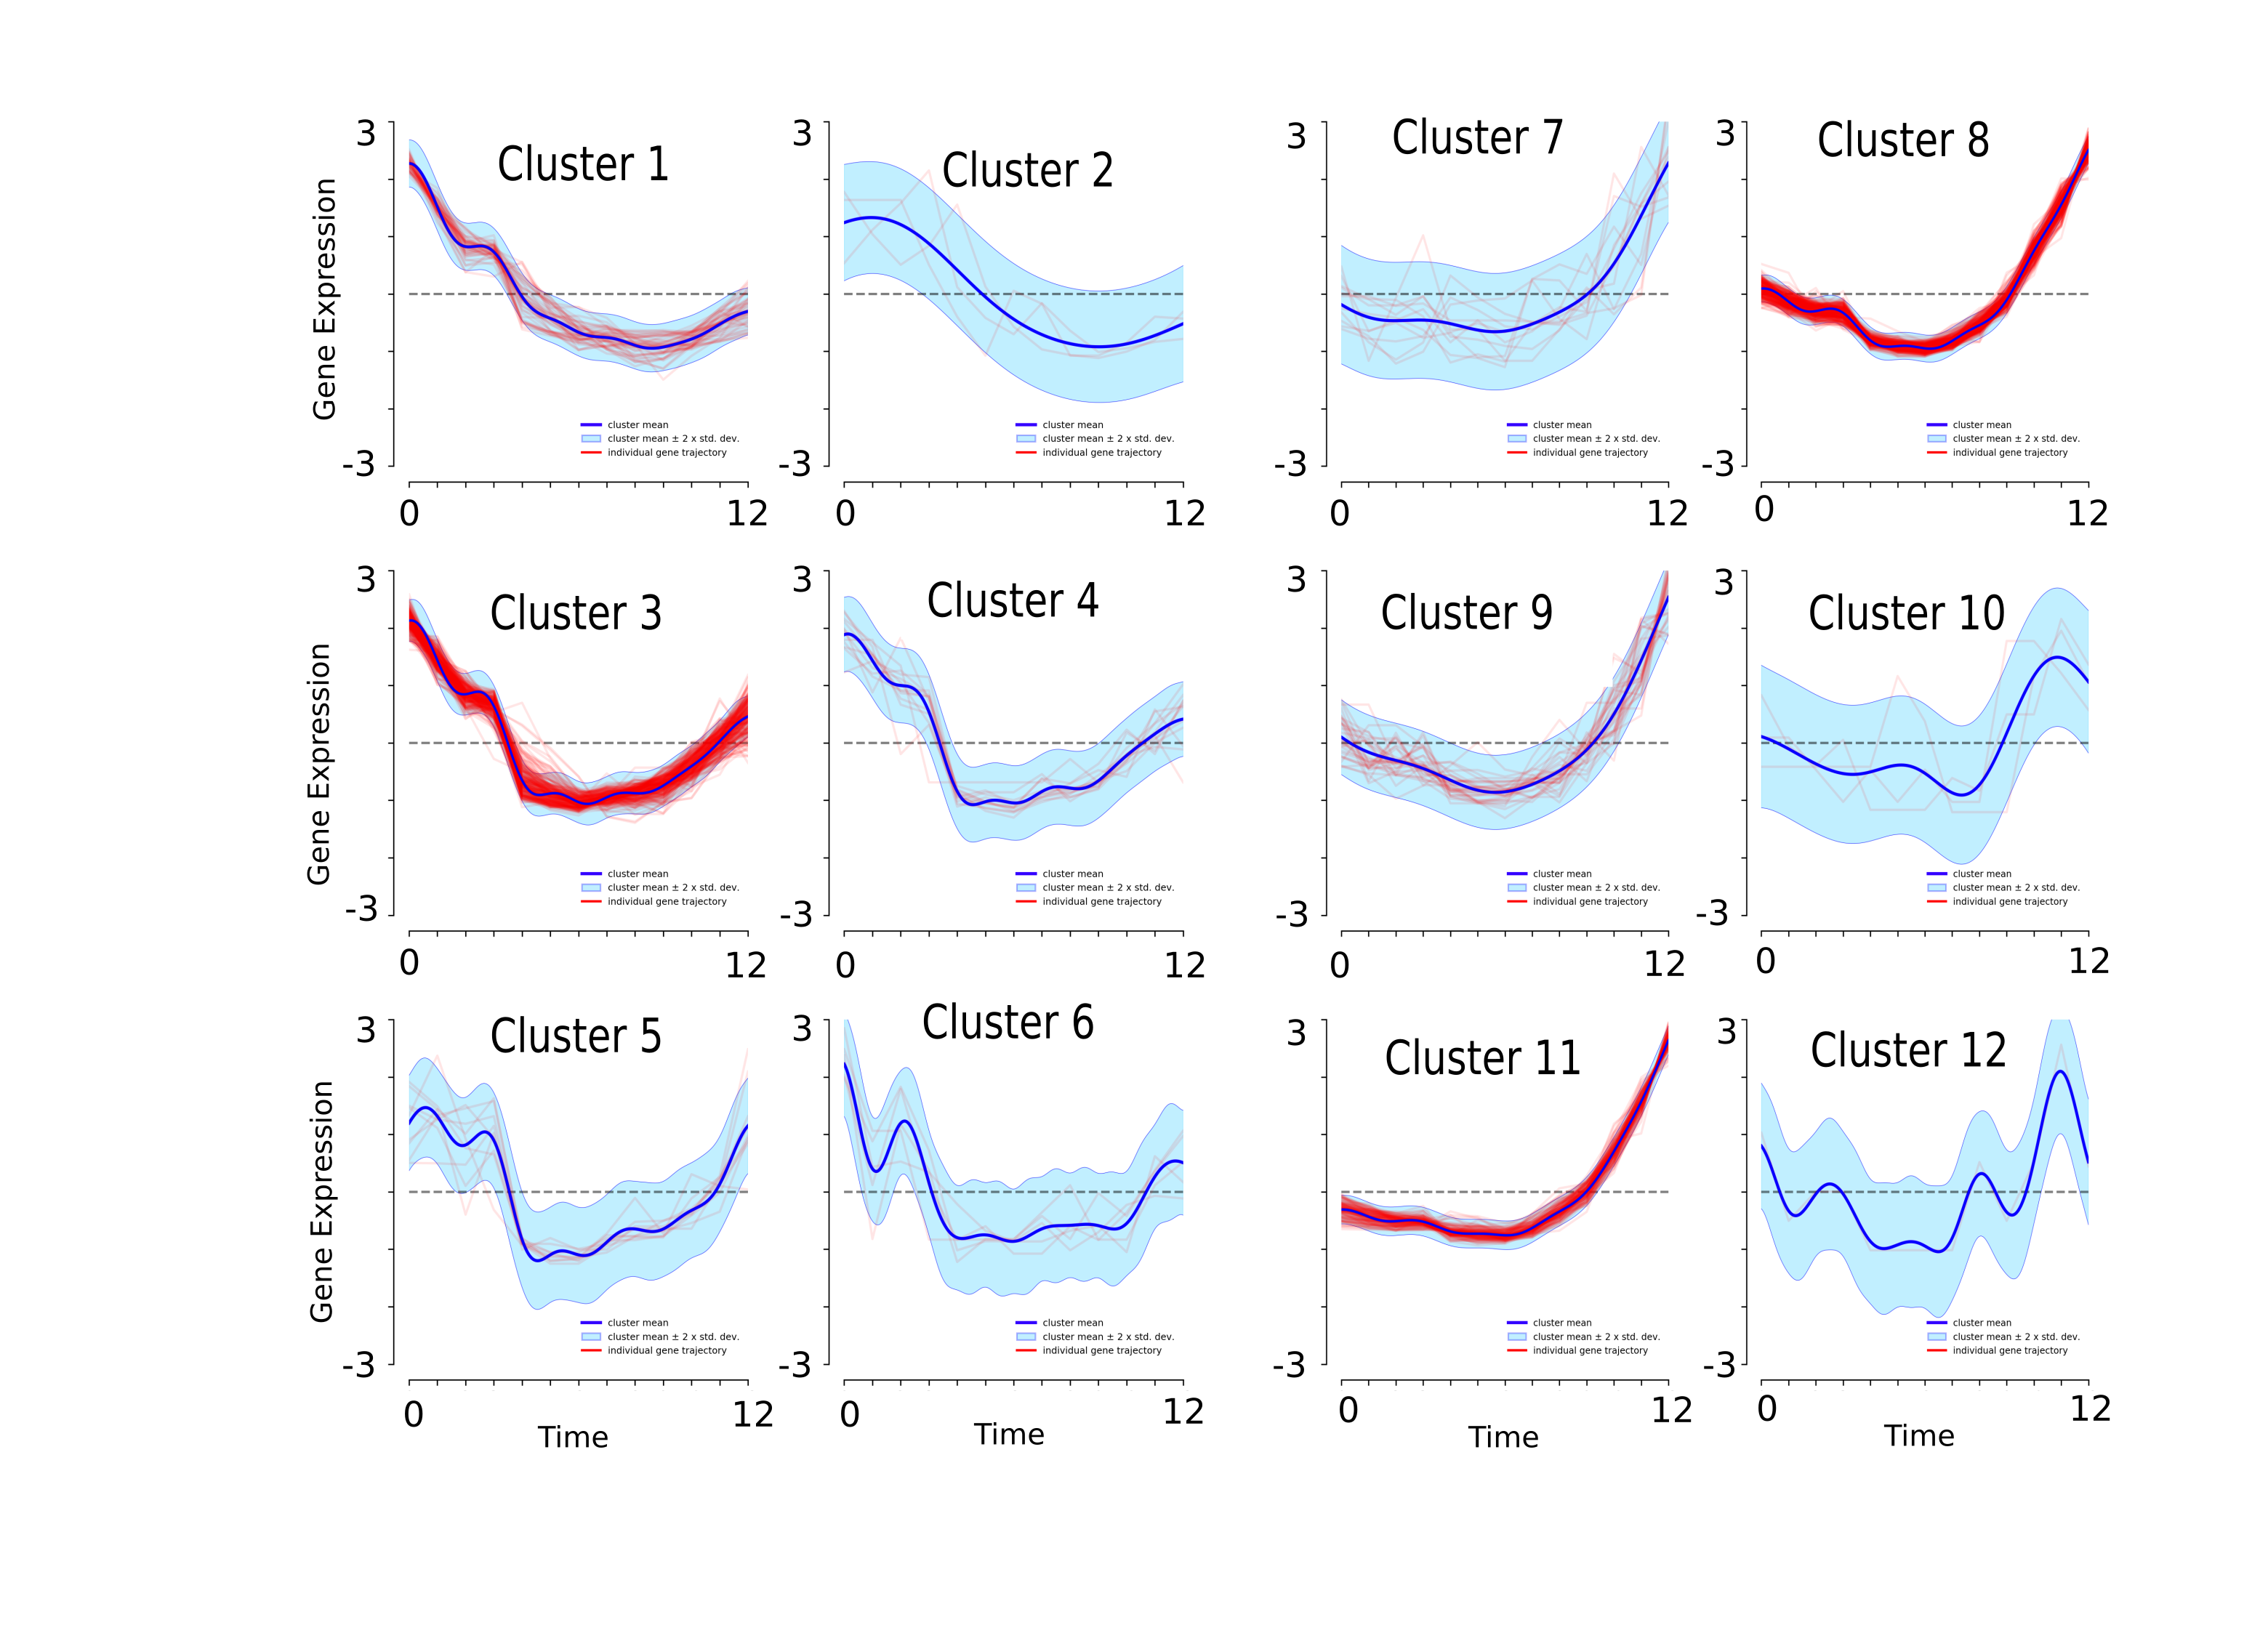
\includegraphics[width=\linewidth,height=0.4\textheight]{figures/fig4.png}
 % archetecture.png: 1149x508 px, 72dpi, 40.53x17.92 cm, bb=0 0 1149 508
    \caption[Clusters detected by the unsupervised clustering algorithm DPGP for ESC differentiation.]{\textbf{Clusters detected by the unsupervised clustering algorithm DPGP for ESC differentiation.} Clusters detected by DPGP in the ESC differentiation dataset  \citep{Klein2015} with default hyperparameters showing cluster means (black), mean $\pm$ 2 s.d. in (blue) and cluster members (red). }
   \label{fig:figS3}
\end{figure}
\end{center}
\newpage
\begin{center}
\begin{figure}
  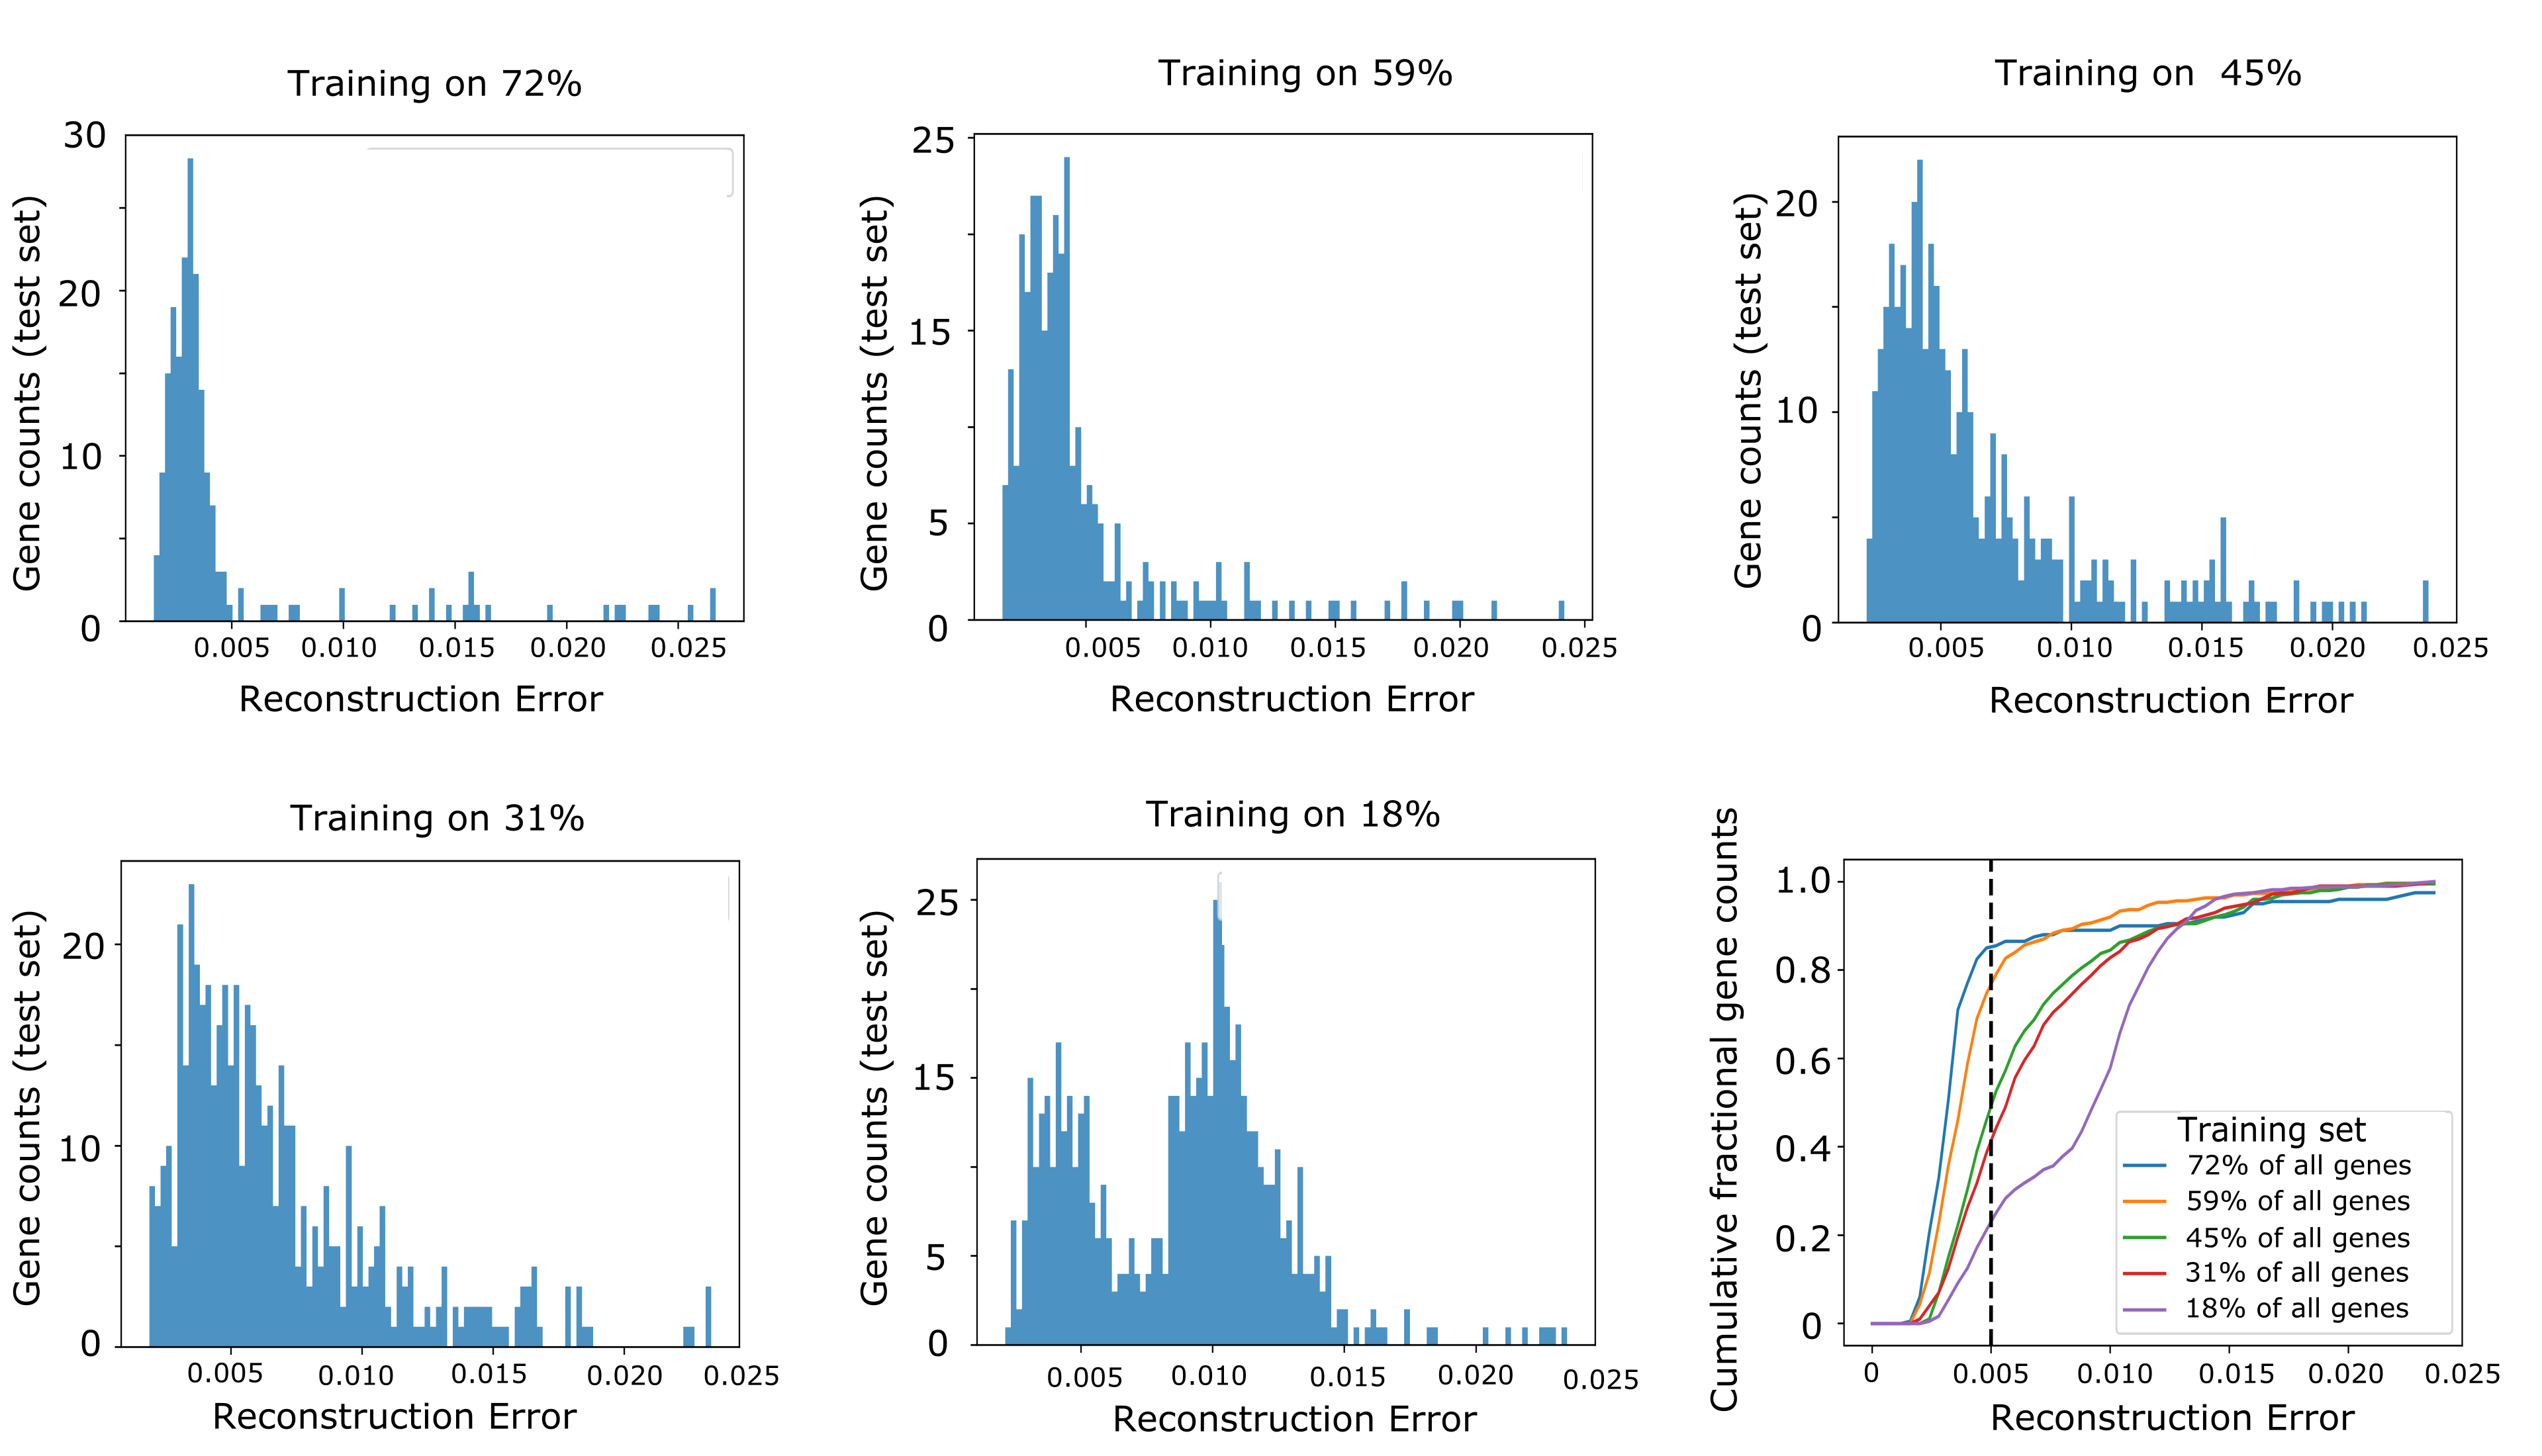
\includegraphics[width=\linewidth]{./figures/supp_varying_test_set_sizes.png}
 % archetecture.png: 1149x508 px, 72dpi, 40.53x17.92 cm, bb=0 0 1149 508
    \caption[Accuracy of RVAgene reconstructions for different train/test group sizes.]{{\bf Accuracy of RVAgene reconstructions for different train/test group sizes.} Distributions of reconstruction errors on randomly sampled sets of test genes, where the full data were split into test groups of: 200 genes (train on 72\%), 300 genes (train on 59\%), 400 genes (train on 45\%), 500 genes (train on 31\%), and 600 genes (train on 18\%). Cumulative fractional distribution of reconstruction errors (cumulative count/test set size) for all groups.}
  \label{fig:figS4}
\end{figure}
\end{center}
\newpage

\begin{center}
\begin{figure}[H]
  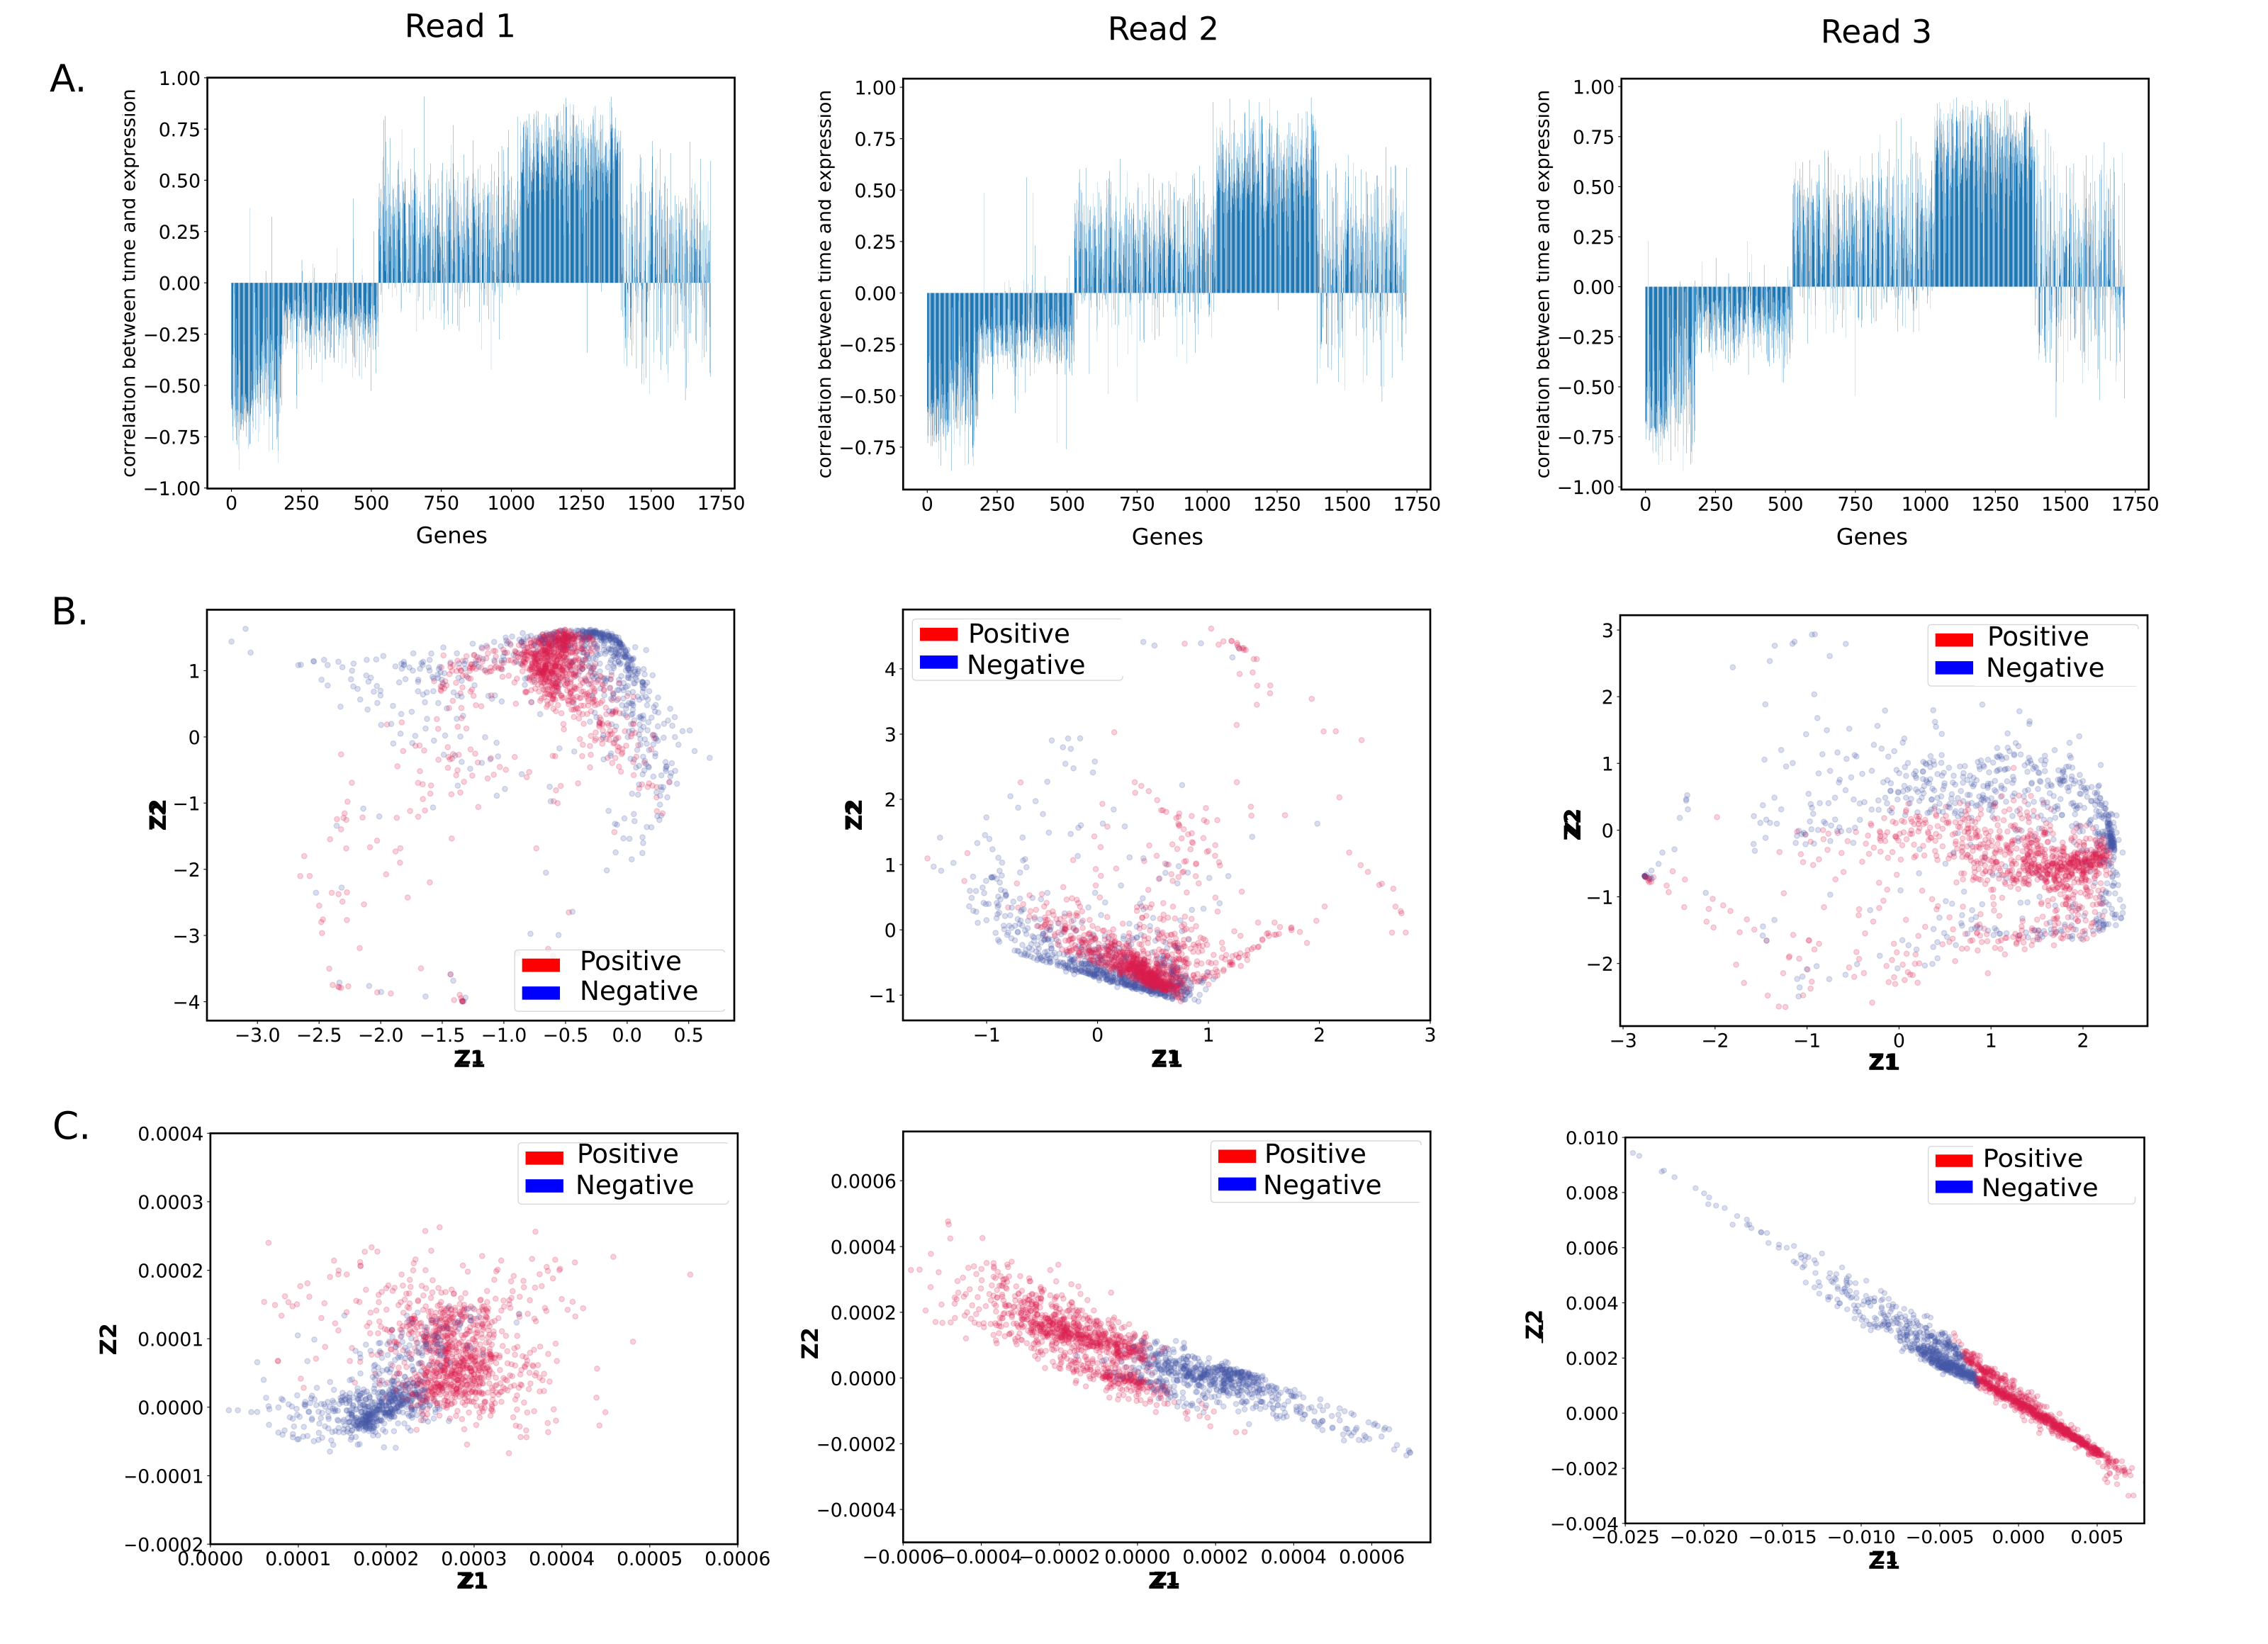
\includegraphics[width = \linewidth]{figures/fig8.png}
 % archetecture.png: 1149x508 px, 72dpi, 40.53x17.92 cm, bb=0 0 1149 508
    \caption[Modeling response to kidney injury and analysis of linear fits.]{\textbf{Modeling response to kidney injury and analysis of linear fits.}
    ({\bf A}) Pearson correlation coefficients between gene expression and time for each differentially expressed gene in the kidney injury dataset for each of the 3 replicates \citep{liu2017molecular}. ({\bf B}) RVAgene latent space representation of fitted model for each replicate; color represents positive or negative correlation coefficients. ({\bf C}) RVAgene latent space representation learnt for the same three replicates as in (B), but where every input gene was normalized  so that its expression sums to 1.}
  \label{fig:figS5}
\end{figure}
\end{center}
\newpage

\begin{center}
\begin{figure}[H]
  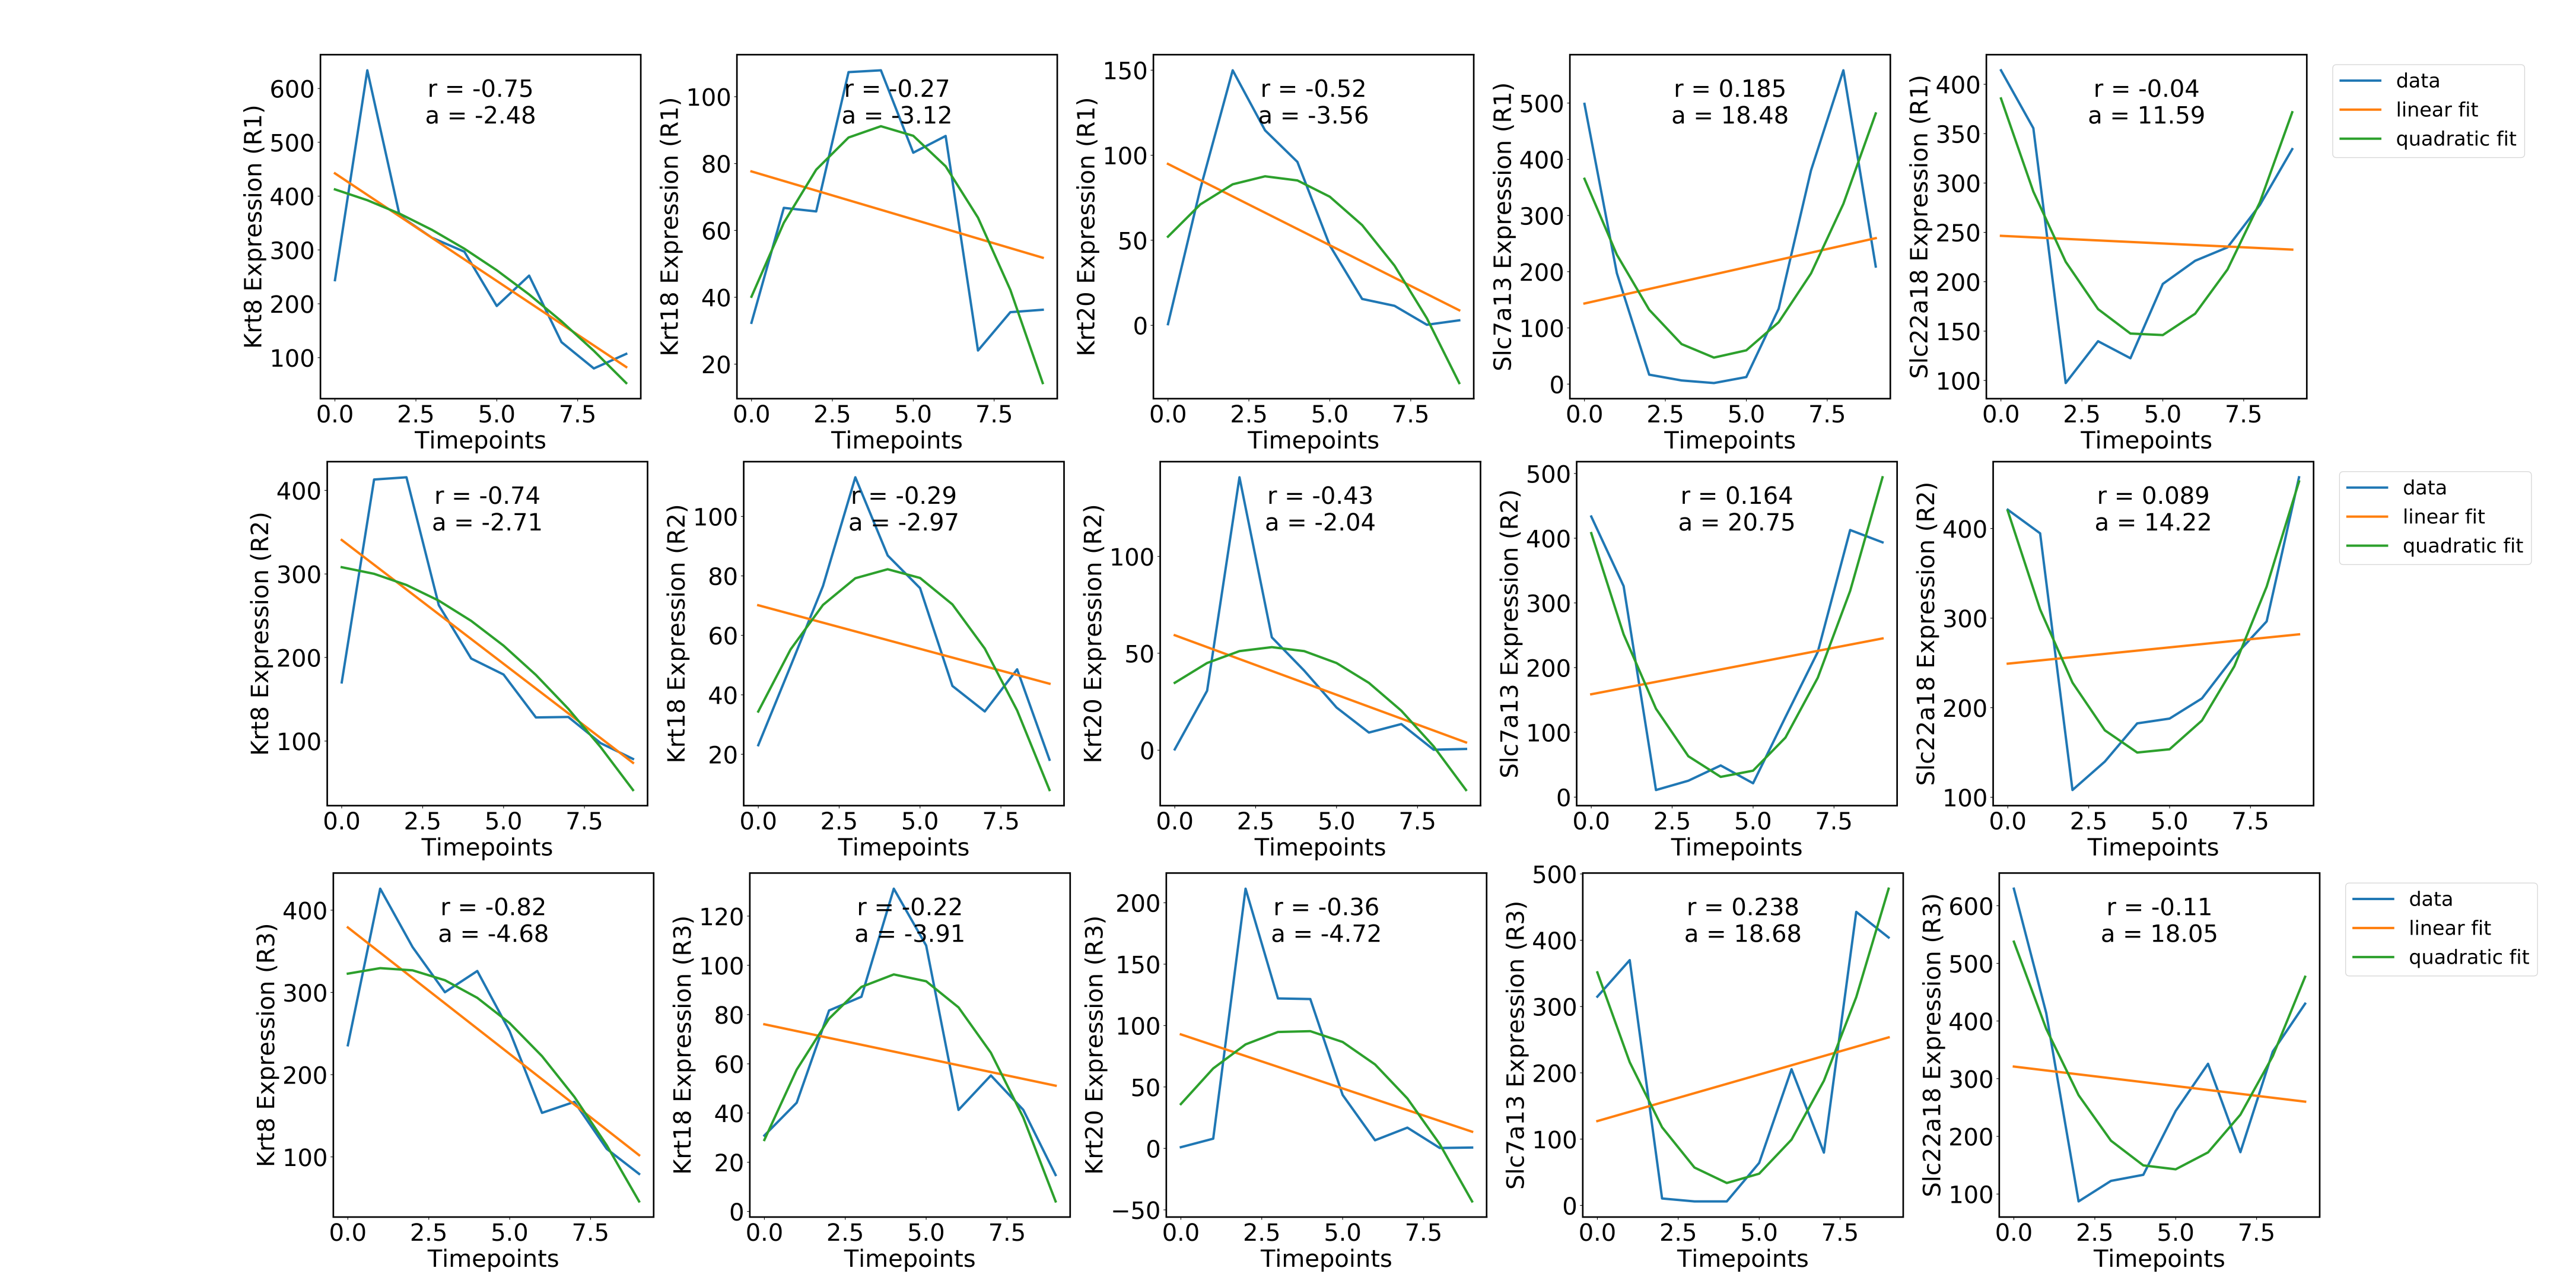
\includegraphics[width=\linewidth]{./figures/sl_JCI_r.png}
 % archetecture.png: 1149x508 px, 72dpi, 40.53x17.92 cm, bb=0 0 1149 508
    \caption[Comparison of linear and quadratic fits to describe gene dynamics in response to kidney injury.]{\textbf{Comparison of linear and quadratic fits to describe gene dynamics in response to kidney injury.}
    For each of the three replicates (R1-R3), five genes are shown, with experimental data (blue), linear fit (orange), and quadratic fit (green). 
    Pearson correlation coefficients, $r$, and quadratic coefficients, $a$ ($x = at^2 + bt + c$), are given for each plot.}
  \label{fig:figS6}
\end{figure}
\end{center}
\newpage

\begin{center}
\begin{figure}[H]
  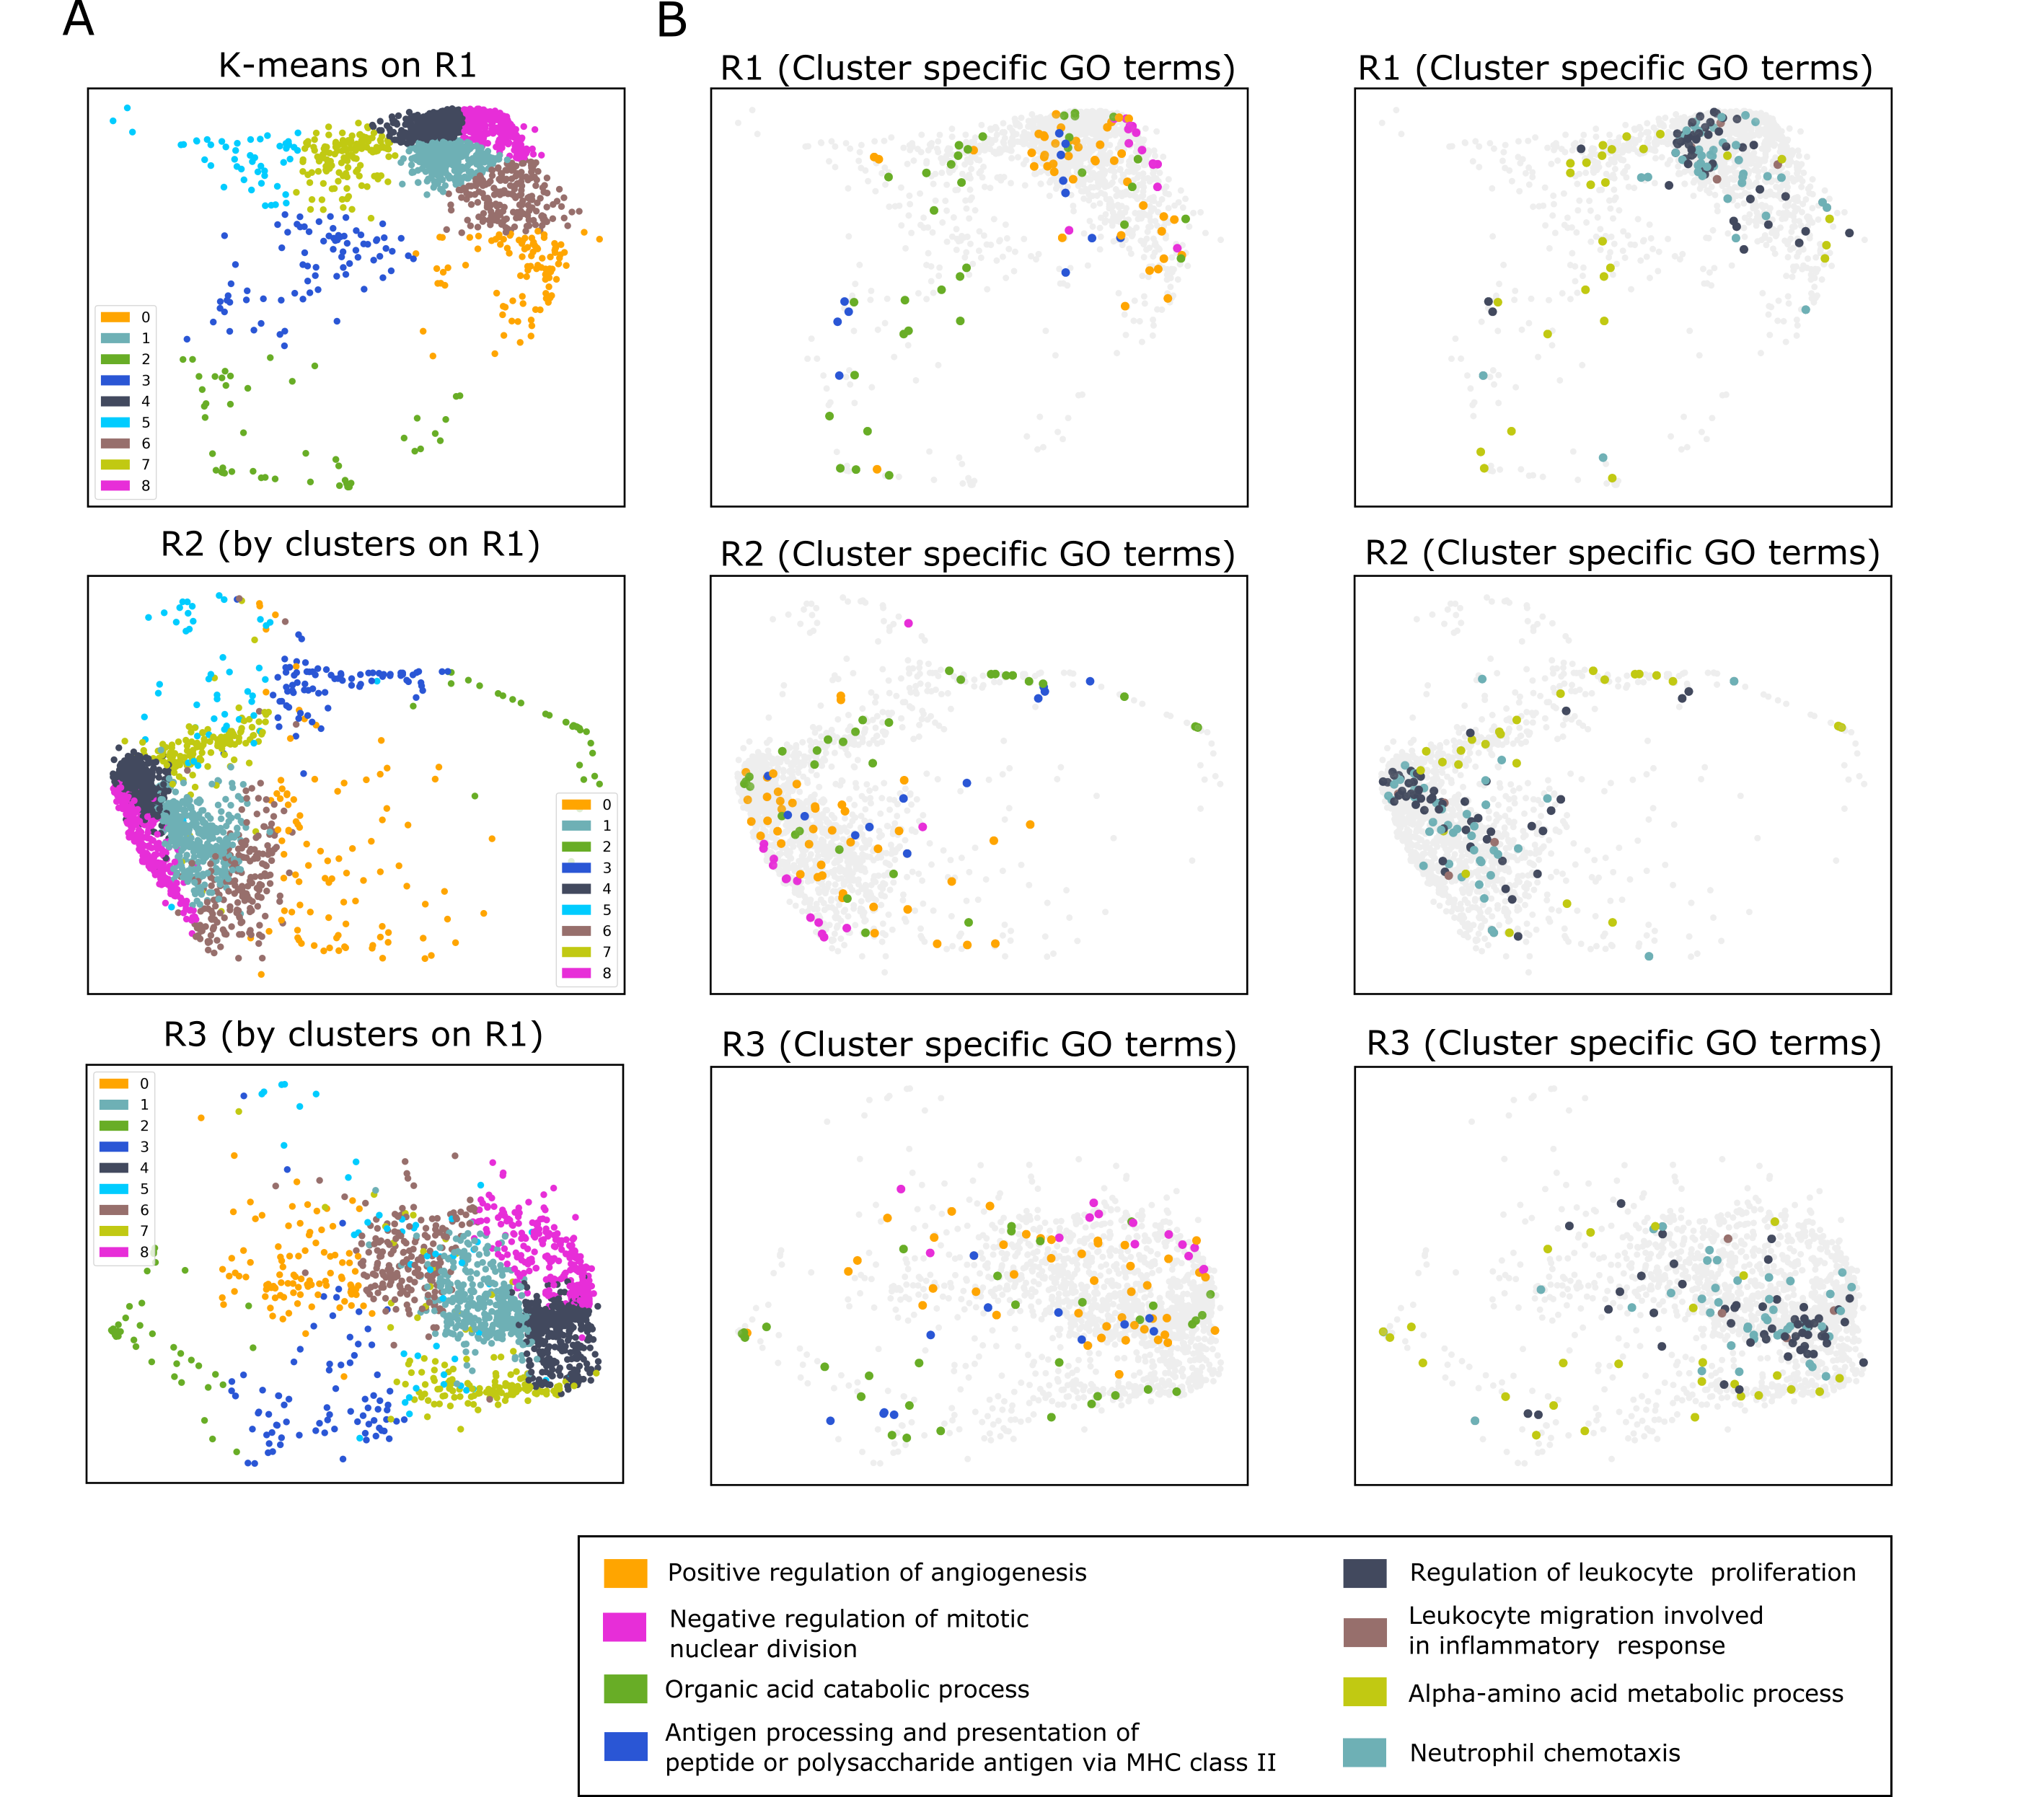
\includegraphics[width=\linewidth]{./figures/supp_go.png}
 % archetecture.png: 1149x508 px, 72dpi, 40.53x17.92 cm, bb=0 0 1149 508
    \caption[Clustering on R1 and cluster specific GO enrichment analysis.]{\textbf{Clustering on R1 and cluster specific GO enrichment analysis.} We performed k-means clustering on latent space learned by RVAgene on R1 with $k=9$. We also show learned latent space on R2 and R3 annotated by the clustering done on R1. All clusters (except cluster 5) appears well preserved. We perform GO analysis for each cluster and select one significant GO term from each cluster (except cluster 5) and show how all genes in the dataset corresponding to each GO term appears on the latent space for all three replicates. }
  \label{fig:figS8}
\end{figure}
\end{center}
\newpage

\begin{center}
\begin{figure}[H]
  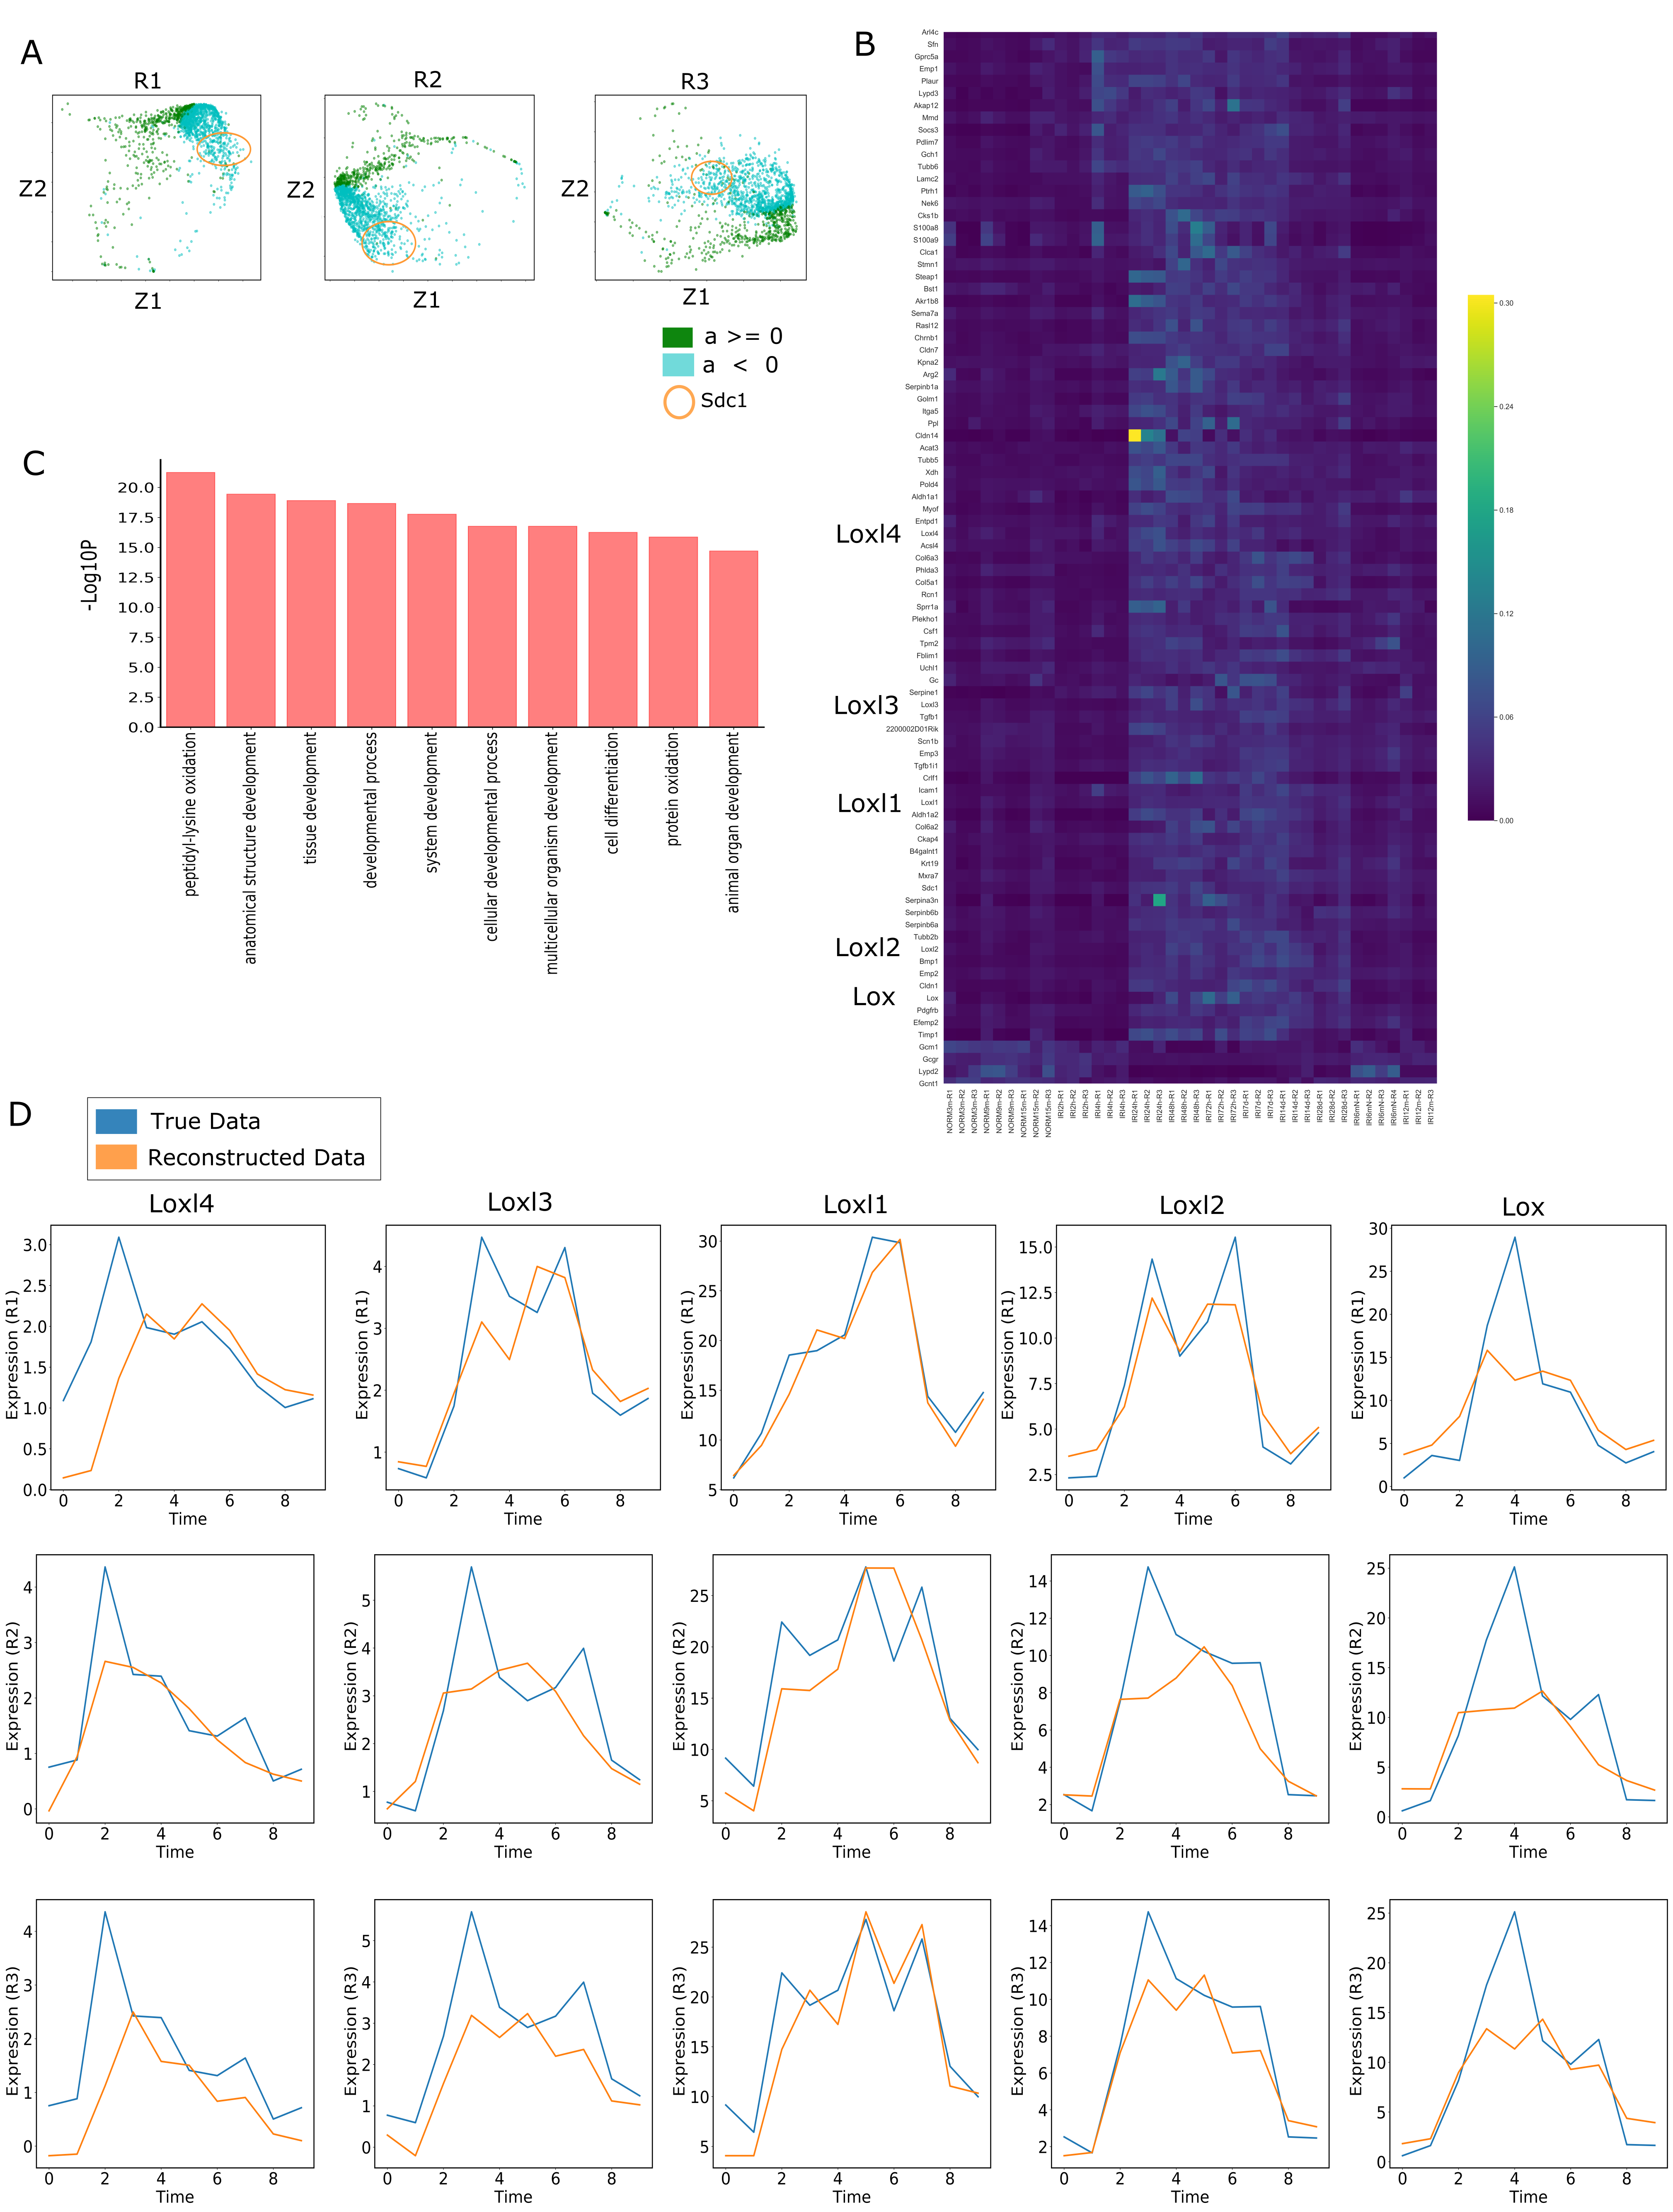
\includegraphics[width=\linewidth]{./figures/sdc_sl.png}
 % archetecture.png: 1149x508 px, 72dpi, 40.53x17.92 cm, bb=0 0 1149 508
    \caption[RVAgene latent space captures biological processes driving concordant gene expression changes (Sdc1).]{{\bf (A)} Latent space representations for replicates R1-R3 with local neighborhoods of Sdc1 marked (circles). ({\bf B}) Heatmap of expression changes over time course of injury for the Sdc1 neighborhood genes in the intersection of R1-R3; selected genes highlighted.  ({\bf C}) Histogram of -log10 p values of top GO terms for biological processes for gene set in (B).
    {\bf D}) Reconstructed vs true data plotted for each of the Lox genes identified in (B).}
  \label{fig:figS7}
\end{figure}
\end{center}

\begin{center}
\begin{figure}[H]
  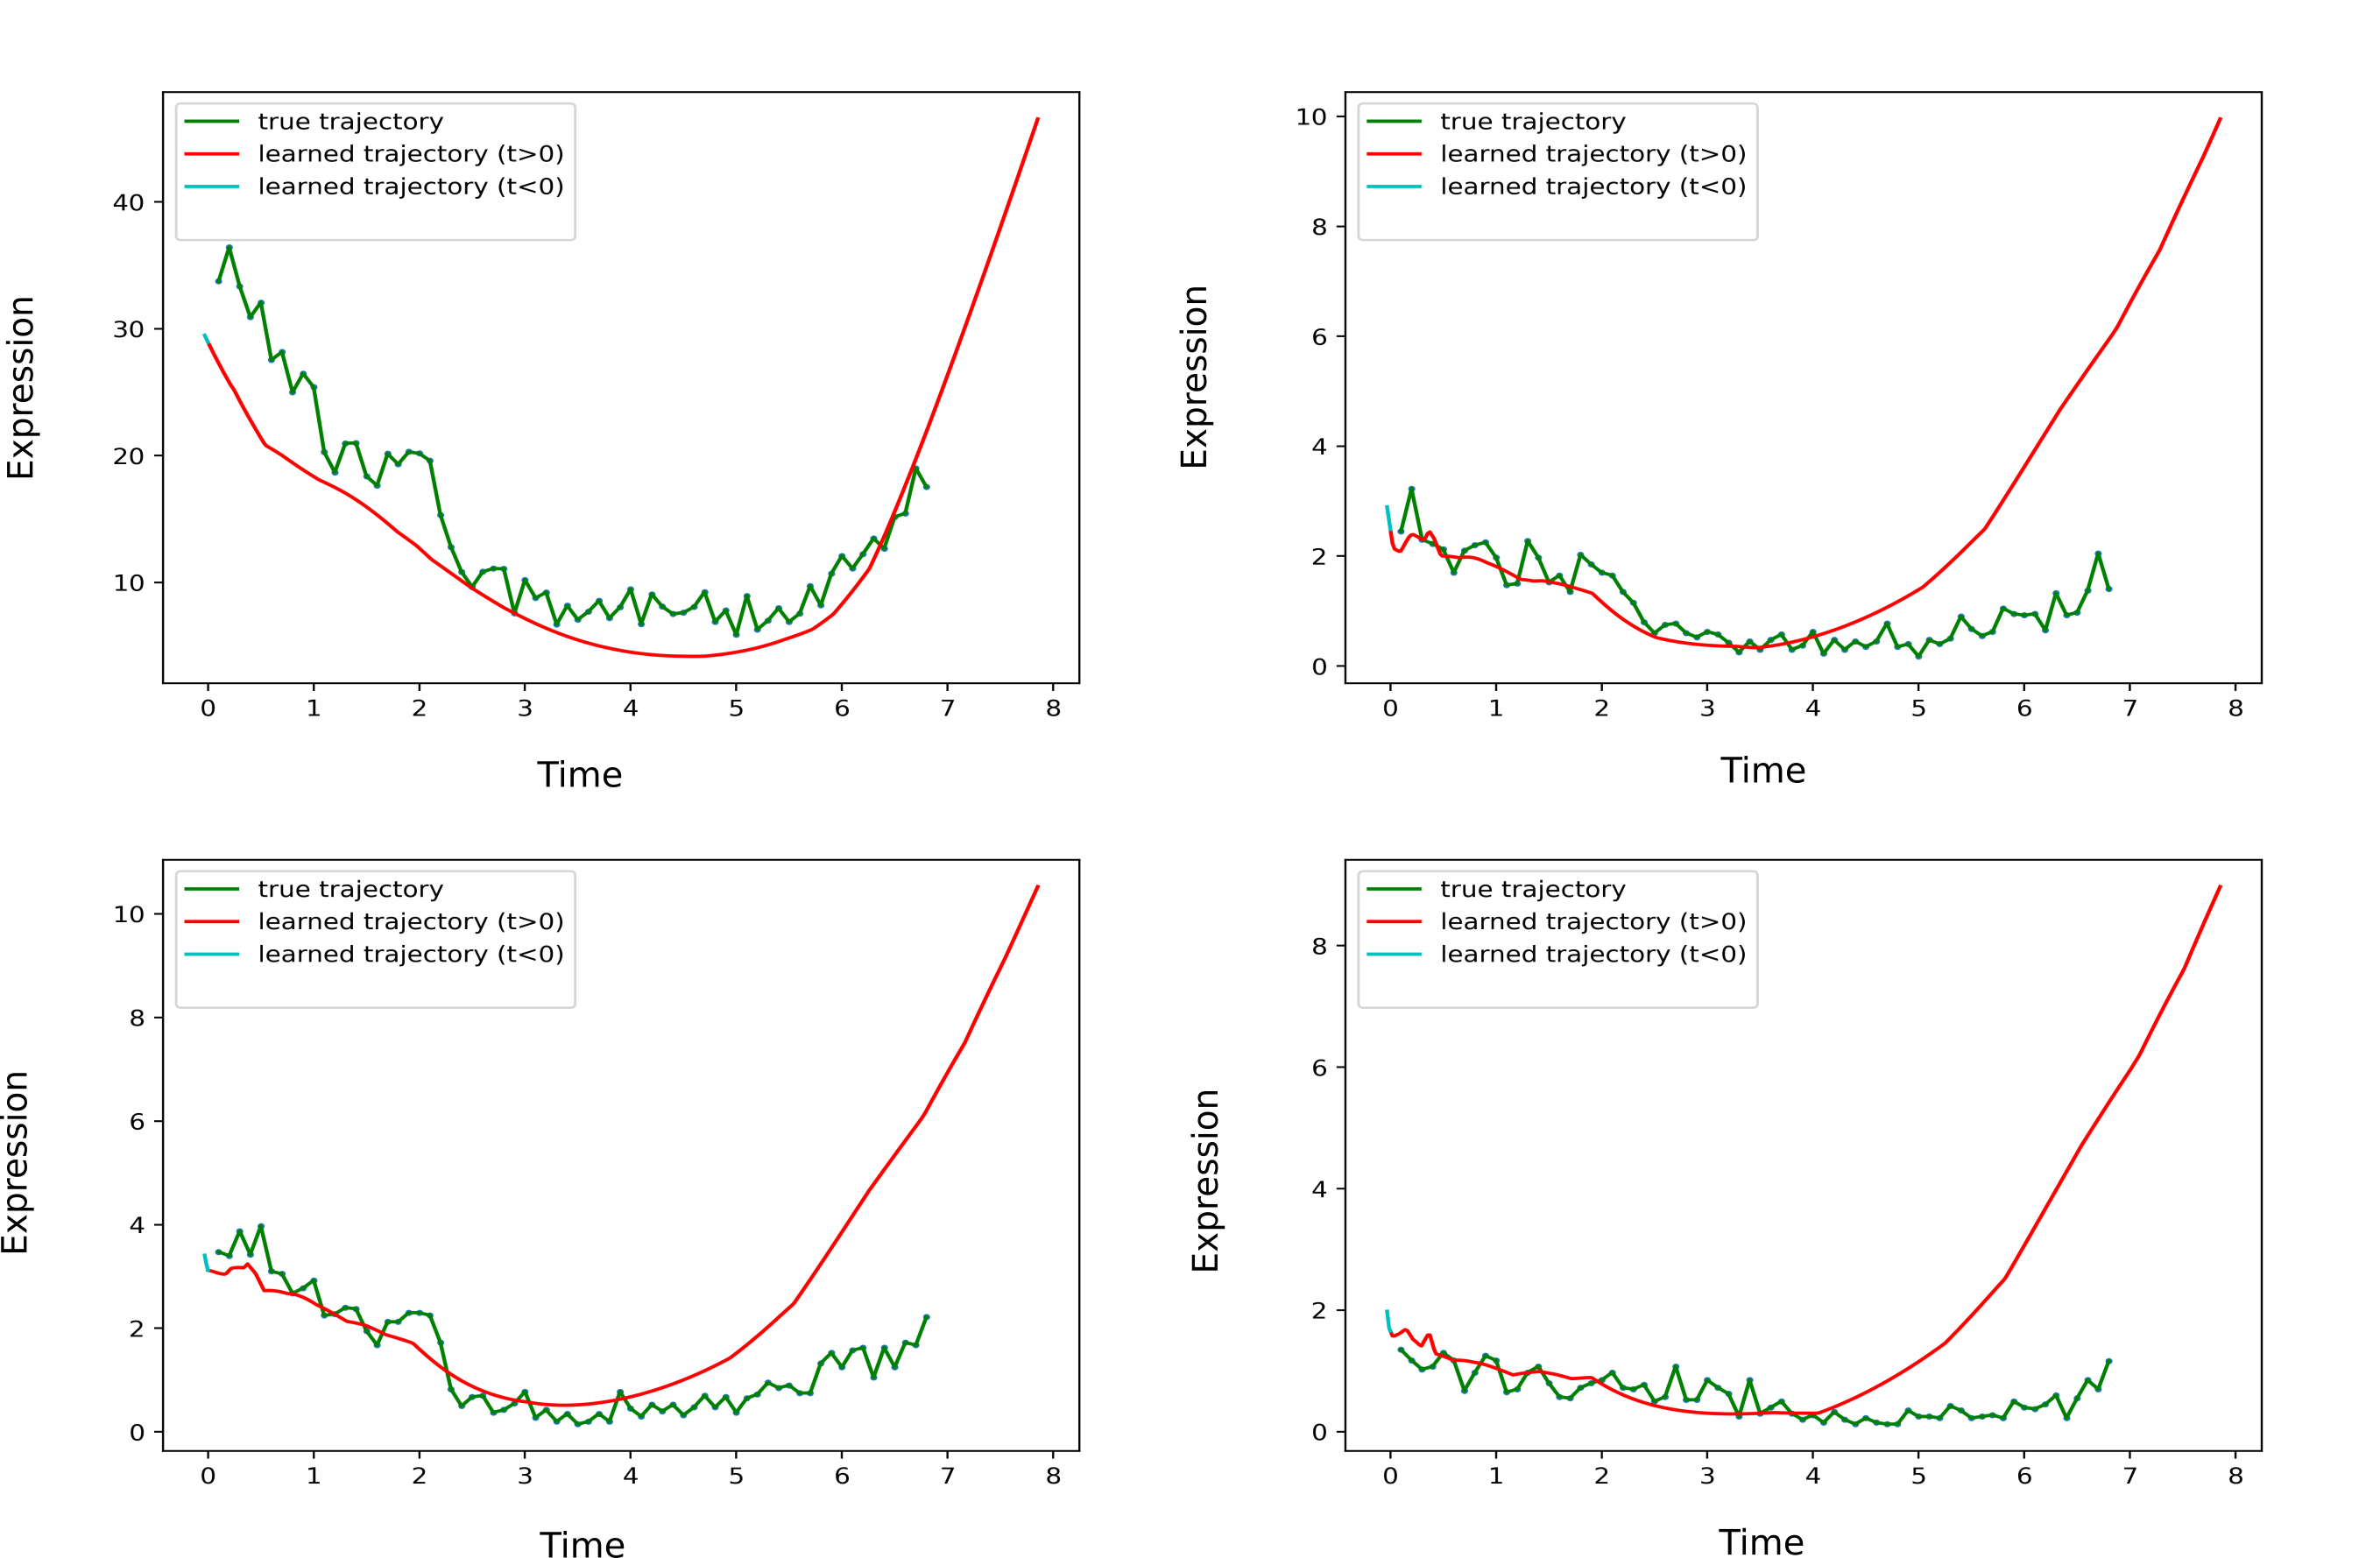
\includegraphics[width=\linewidth]{./figures/latent_ode_val_underfit.png}
 % archetecture.png: 1149x508 px, 72dpi, 40.53x17.92 cm, bb=0 0 1149 508
    \caption[Examples of continuous time prediction of ESC differentiation.]{\textbf{Examples of continuous time prediction of ESC differentiation.} Reconstruction (up to $t=6.8$) and future prediction (for $t>6.8$) for 4 example genes by a  latent ODE \citep{chen2018neural} trained on ESC data \citep{Klein2015} for 1000000 iterations, showing a good fit for the initial timepoints, but underfitting for the later timepoints.}
  \label{fig:figS9}
\end{figure}
\end{center}

%% RNASCAPE SUPP FIGURES
\begin{center}
\begin{figure}[H]
  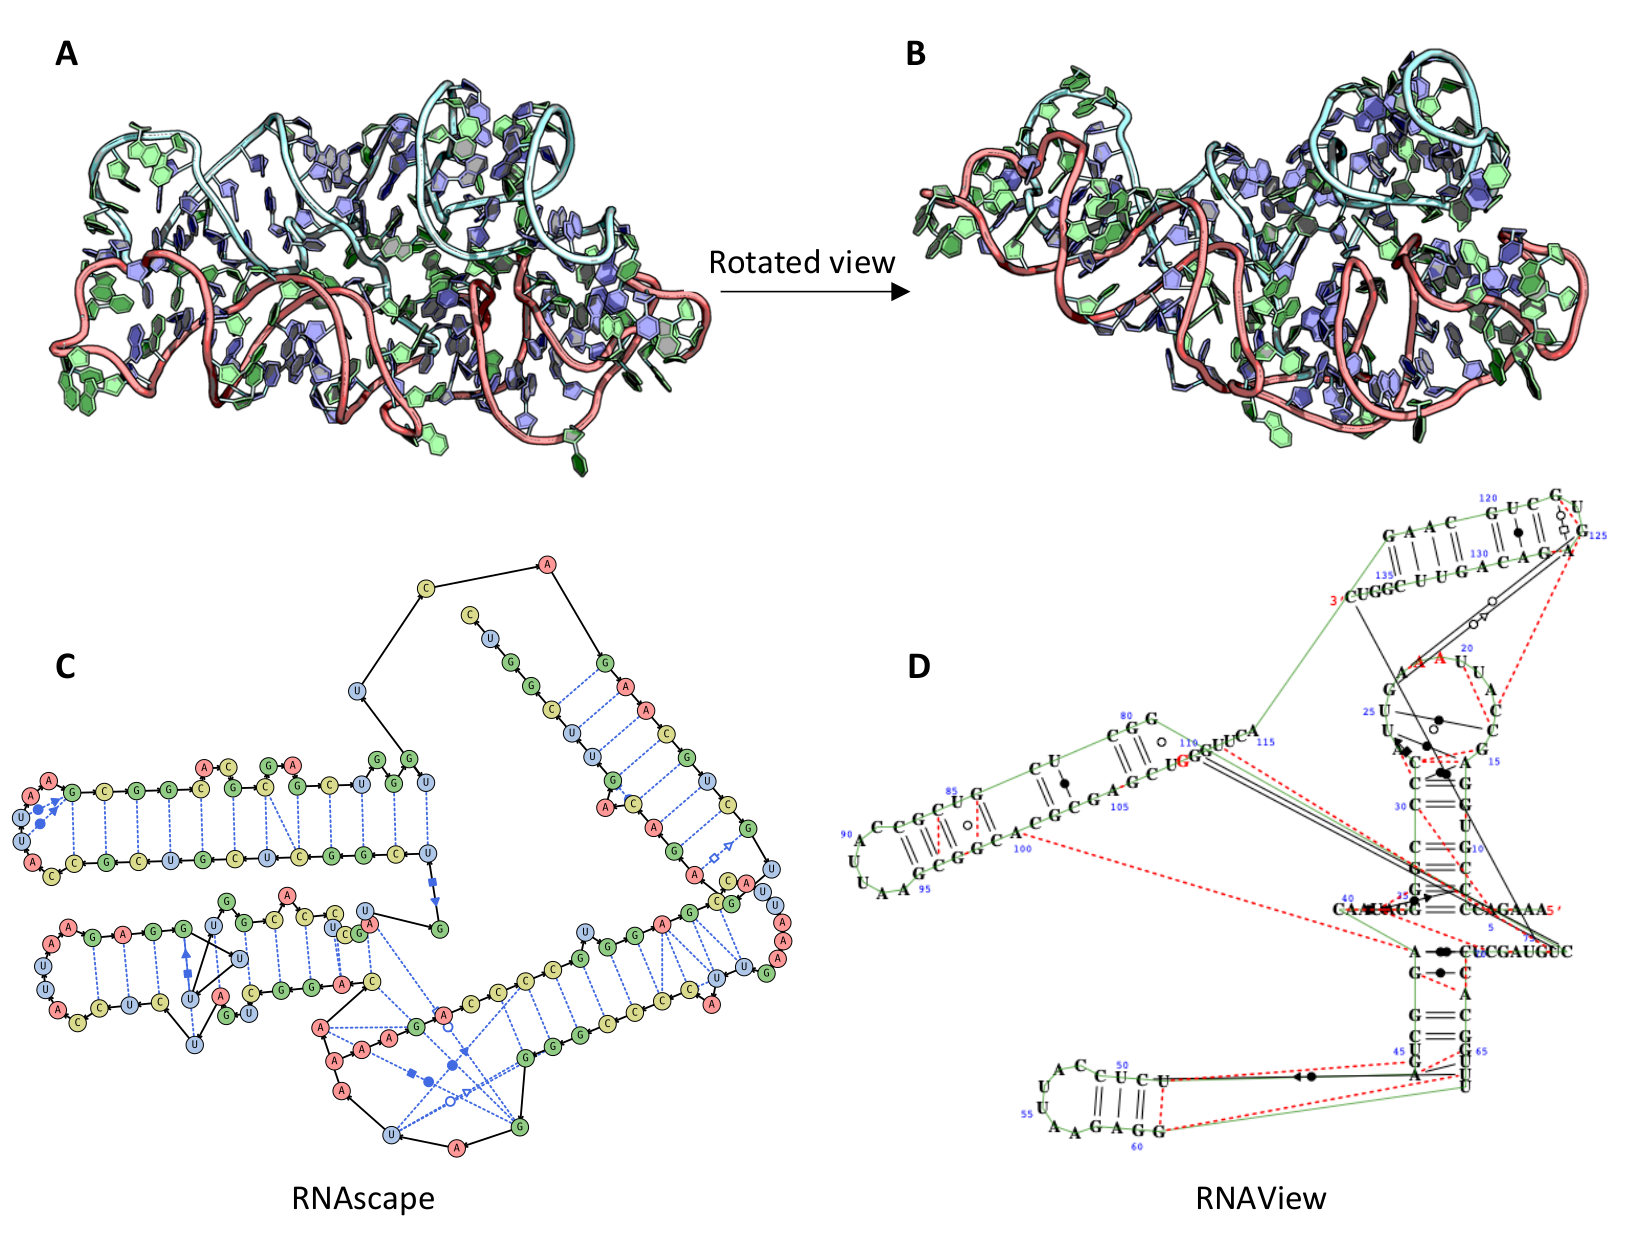
\includegraphics[width=\linewidth]{./rnascapefigs/figureS1.png}
 % archetecture.png: 1149x508 px, 72dpi, 40.53x17.92 cm, bb=0 0 1149 508
    \caption[Examples of continuous time prediction of ESC differentiation.]{\textbf{Examples of continuous time prediction of ESC differentiation.} Reconstruction (up to $t=6.8$) and future prediction (for $t>6.8$) for 4 example genes by a  latent ODE \citep{chen2018neural} trained on ESC data \citep{Klein2015} for 1000000 iterations, showing a good fit for the initial timepoints, but underfitting for the later timepoints.}
  \label{fig:rnascapeS1}
\end{figure}
\end{center}

\begin{center}
\begin{figure}[H]
  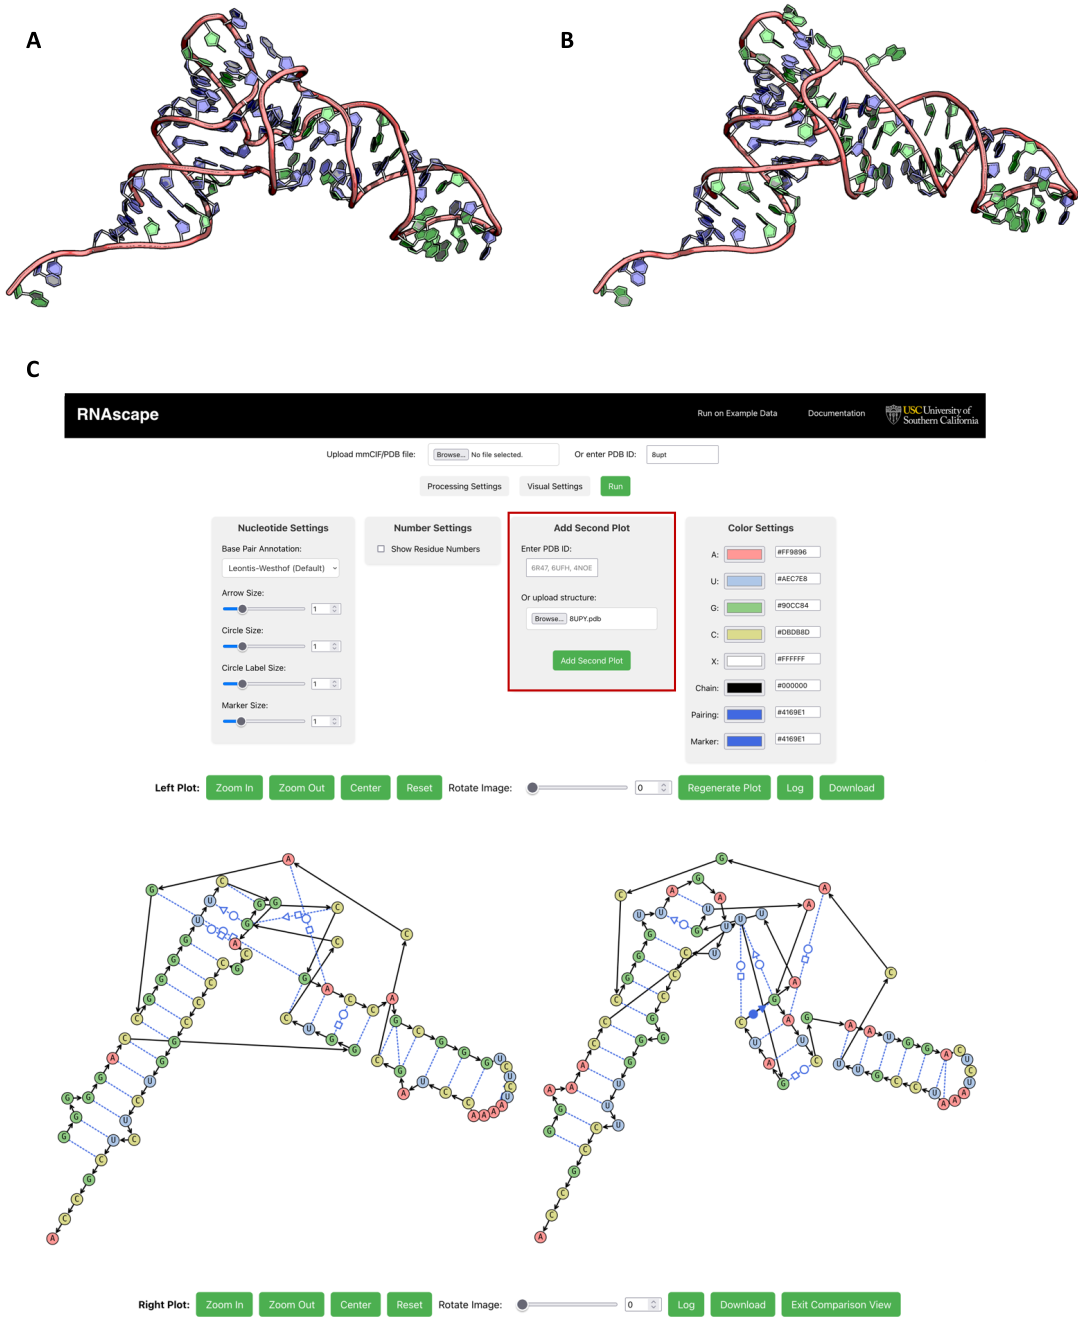
\includegraphics[width=\linewidth]{./rnascapefigs/figureS2.png}
 % archetecture.png: 1149x508 px, 72dpi, 40.53x17.92 cm, bb=0 0 1149 508
    \caption[Examples of continuous time prediction of ESC differentiation.]{\textbf{Examples of continuous time prediction of ESC differentiation.} Reconstruction (up to $t=6.8$) and future prediction (for $t>6.8$) for 4 example genes by a  latent ODE \citep{chen2018neural} trained on ESC data \citep{Klein2015} for 1000000 iterations, showing a good fit for the initial timepoints, but underfitting for the later timepoints.}
  \label{fig:rnascapeS2}
\end{figure}
\end{center}

\begin{center}
\begin{figure}[H]
  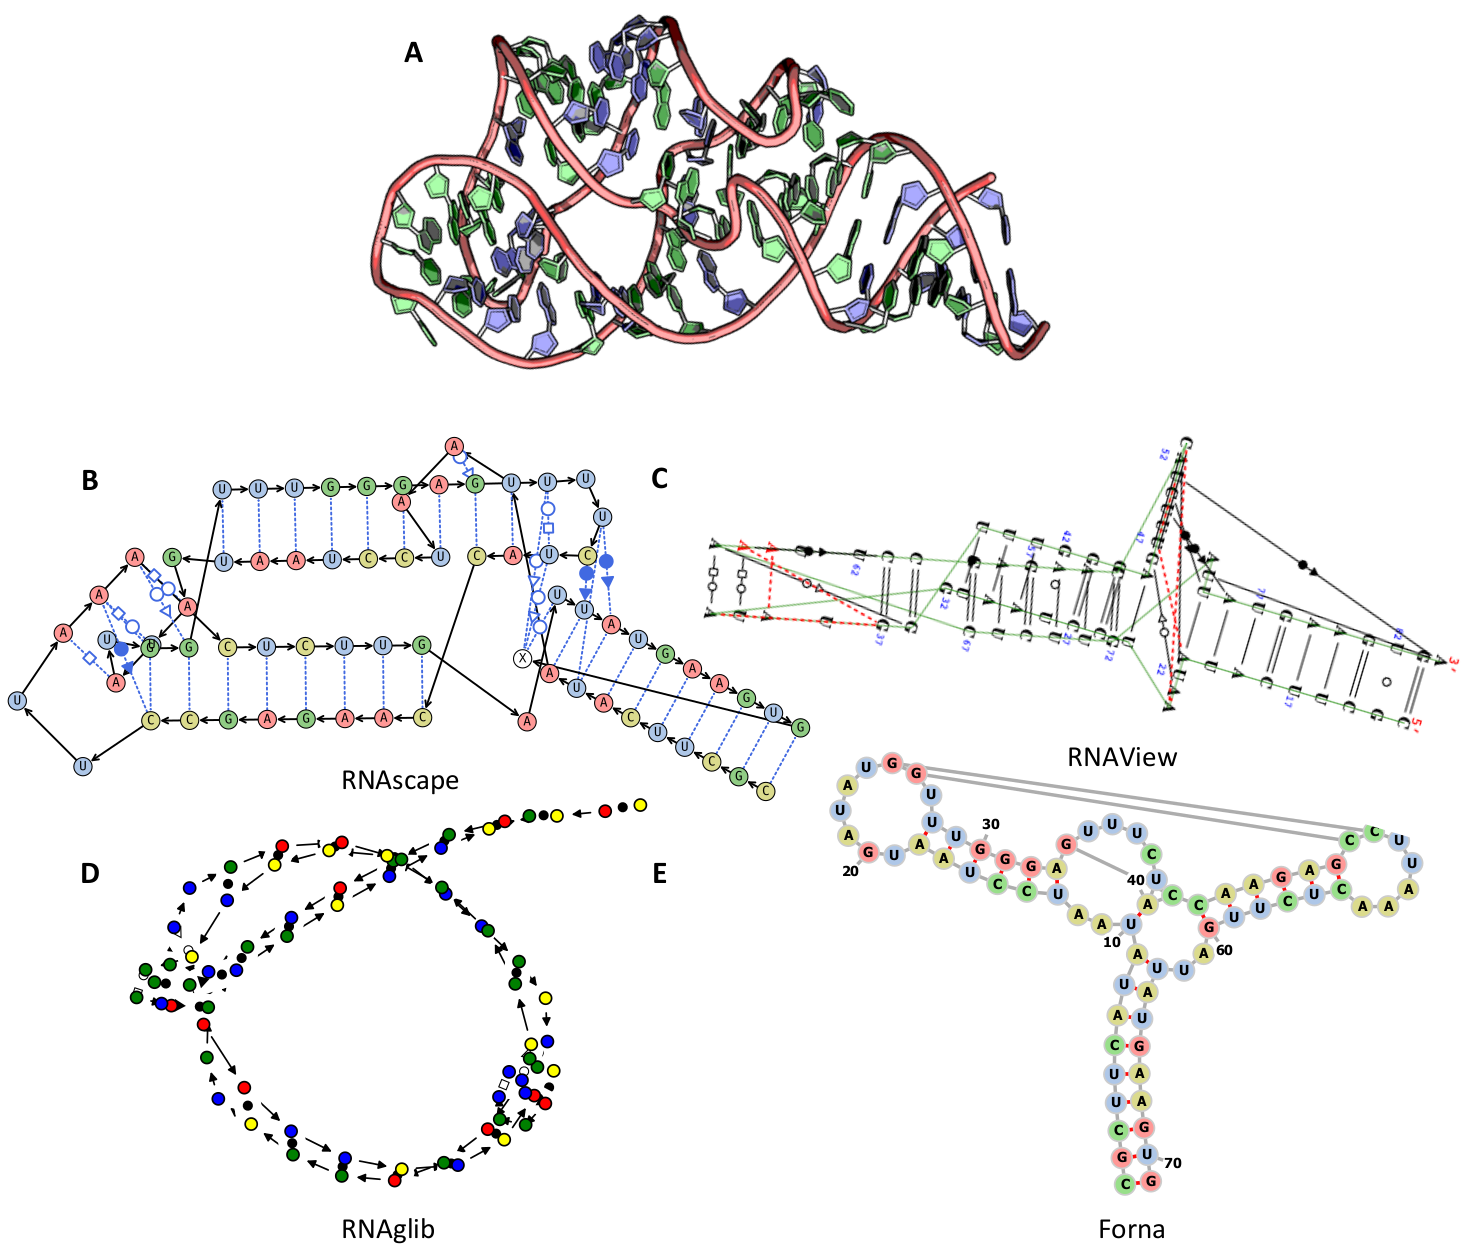
\includegraphics[width=\linewidth]{./rnascapefigs/figureS3.png}
 % archetecture.png: 1149x508 px, 72dpi, 40.53x17.92 cm, bb=0 0 1149 508
    \caption[Examples of continuous time prediction of ESC differentiation.]{\textbf{Examples of continuous time prediction of ESC differentiation.} Reconstruction (up to $t=6.8$) and future prediction (for $t>6.8$) for 4 example genes by a  latent ODE \citep{chen2018neural} trained on ESC data \citep{Klein2015} for 1000000 iterations, showing a good fit for the initial timepoints, but underfitting for the later timepoints.}
  \label{fig:rnascapeS3}
\end{figure}
\end{center}

%% DeepPBS SUPP FIGURES
\begin{center}
\begin{figure}[H]
  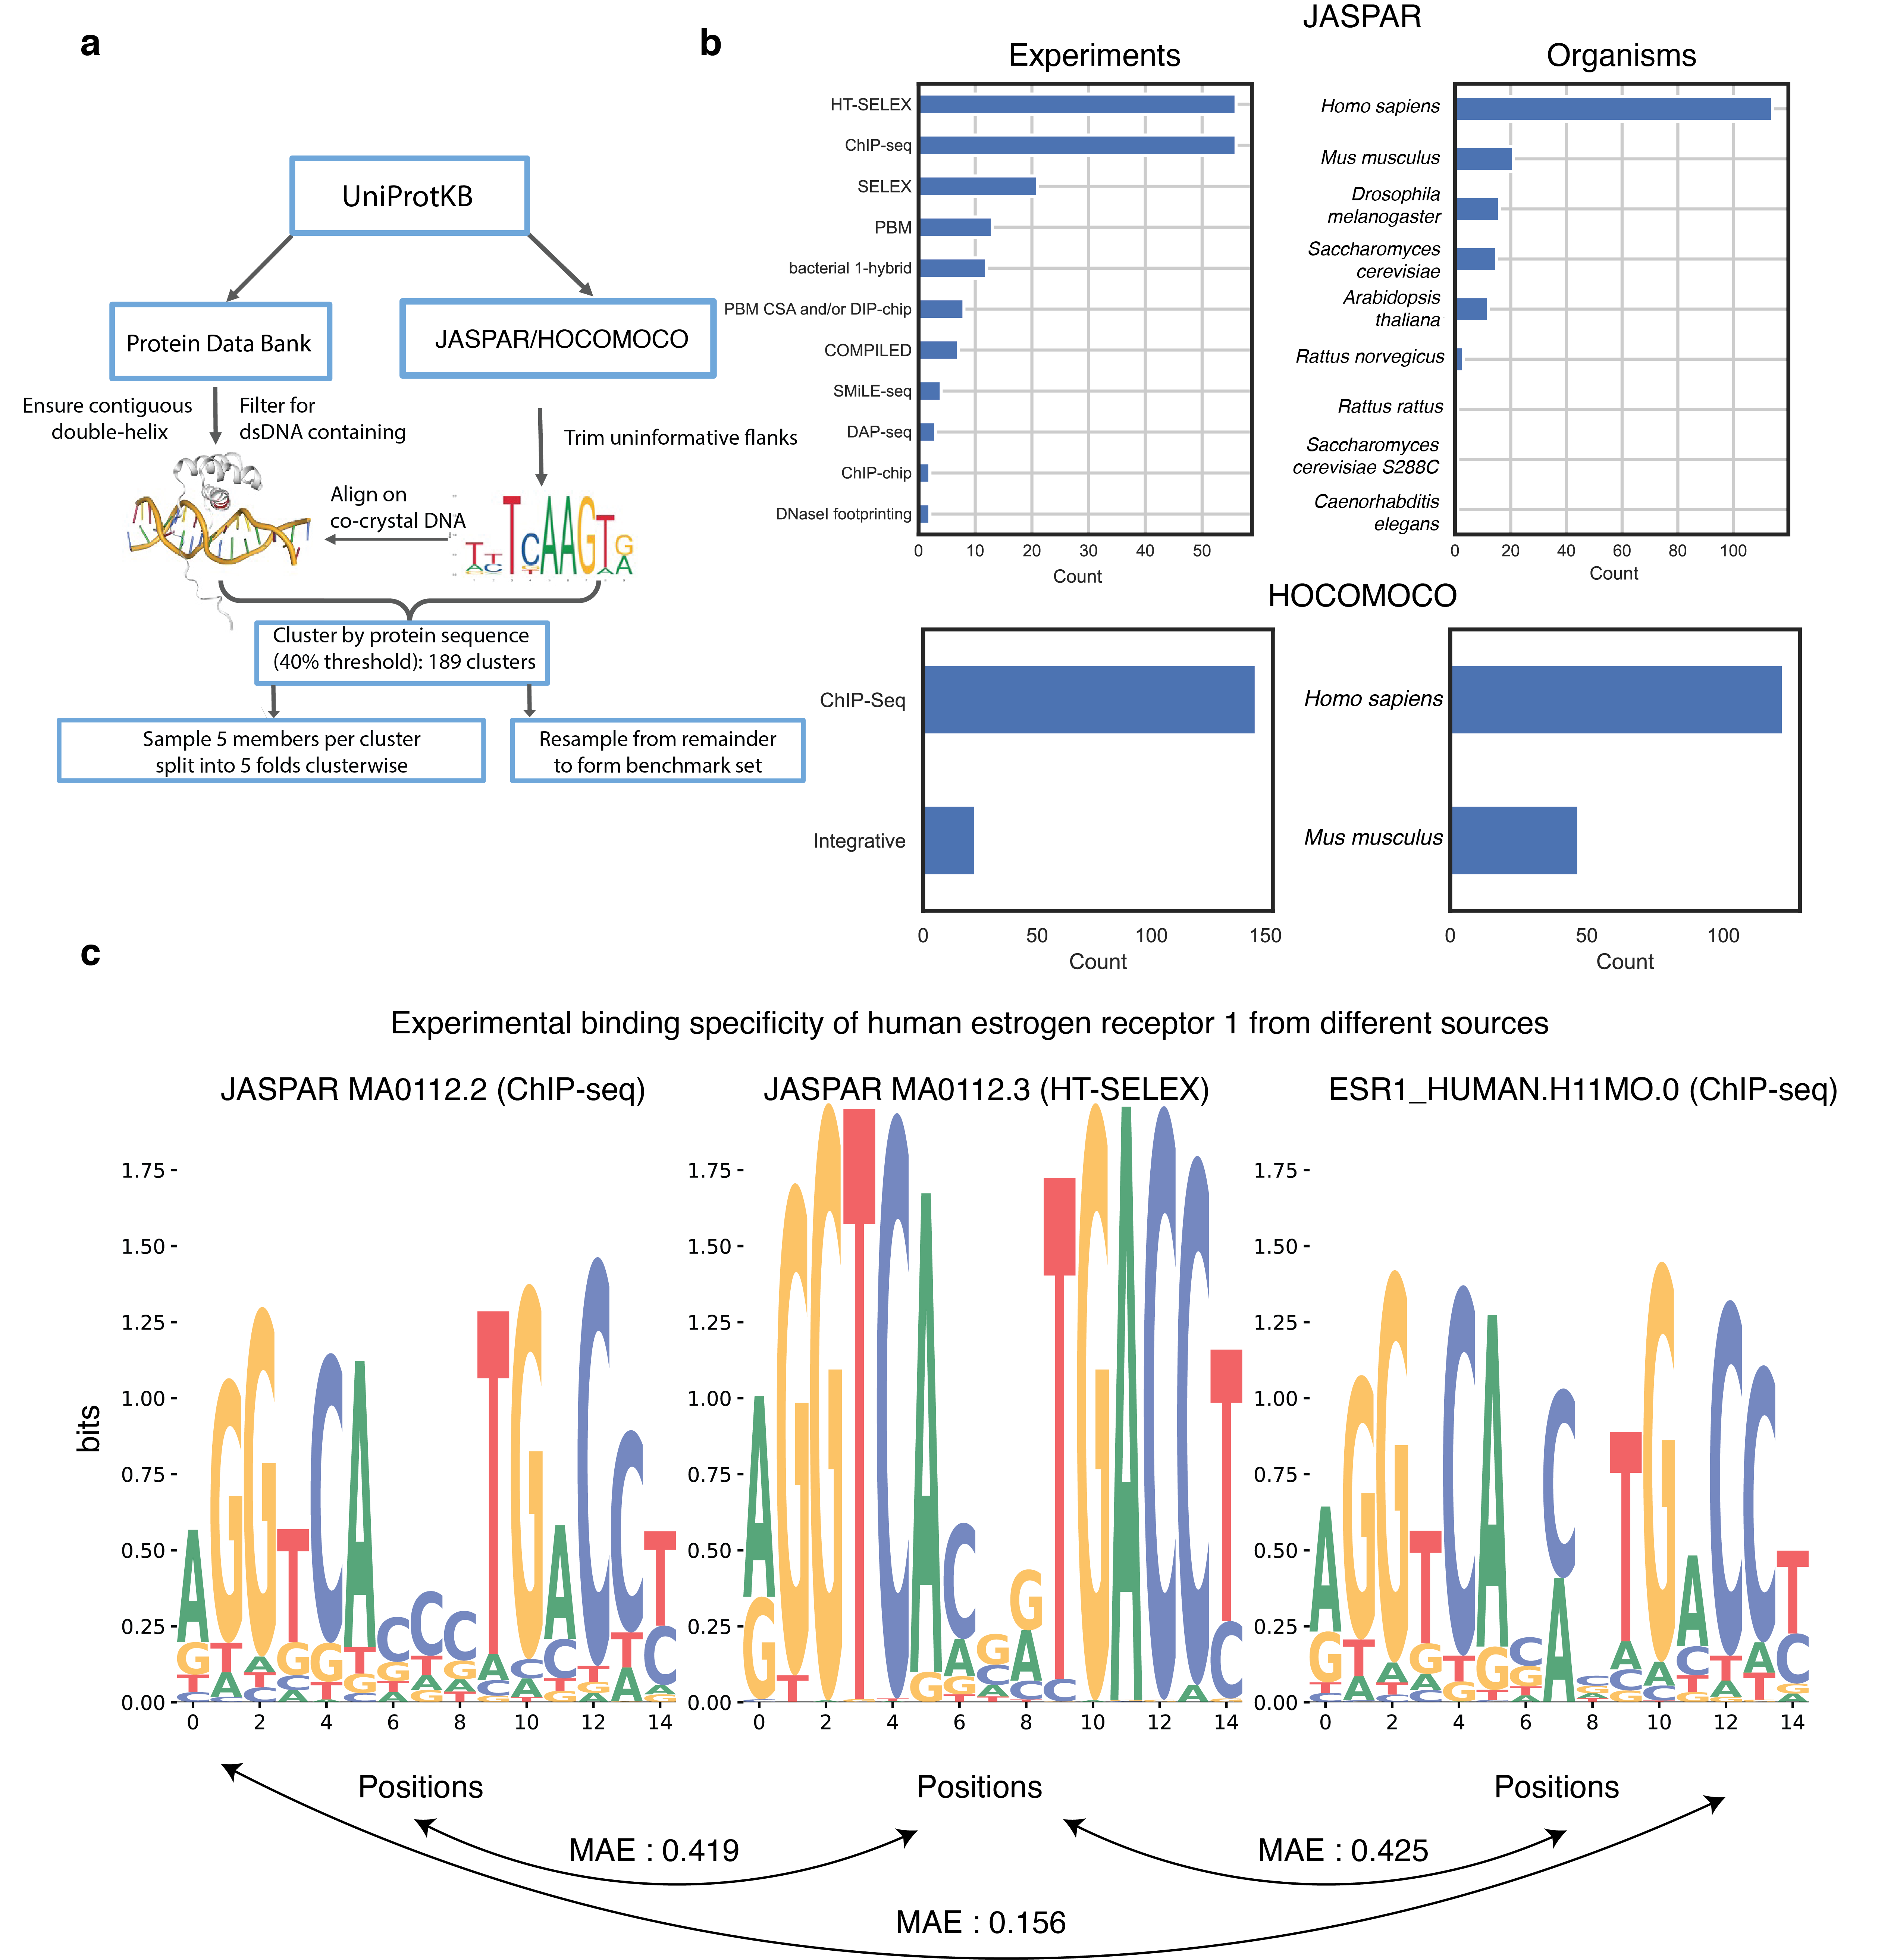
\includegraphics[width=\linewidth]{./pdnafigs/figS1.png}
 % archetecture.png: 1149x508 px, 72dpi, 40.53x17.92 cm, bb=0 0 1149 508
    \caption[Examples of continuous time prediction of ESC differentiation.]{\textbf{Examples of continuous time prediction of ESC differentiation.} Reconstruction (up to $t=6.8$) and future prediction (for $t>6.8$) for 4 example genes by a  latent ODE \citep{chen2018neural} trained on ESC data \citep{Klein2015} for 1000000 iterations, showing a good fit for the initial timepoints, but underfitting for the later timepoints.}
  \label{fig:pdnaS1}
\end{figure}
\end{center}

\begin{center}
\begin{figure}[H]
  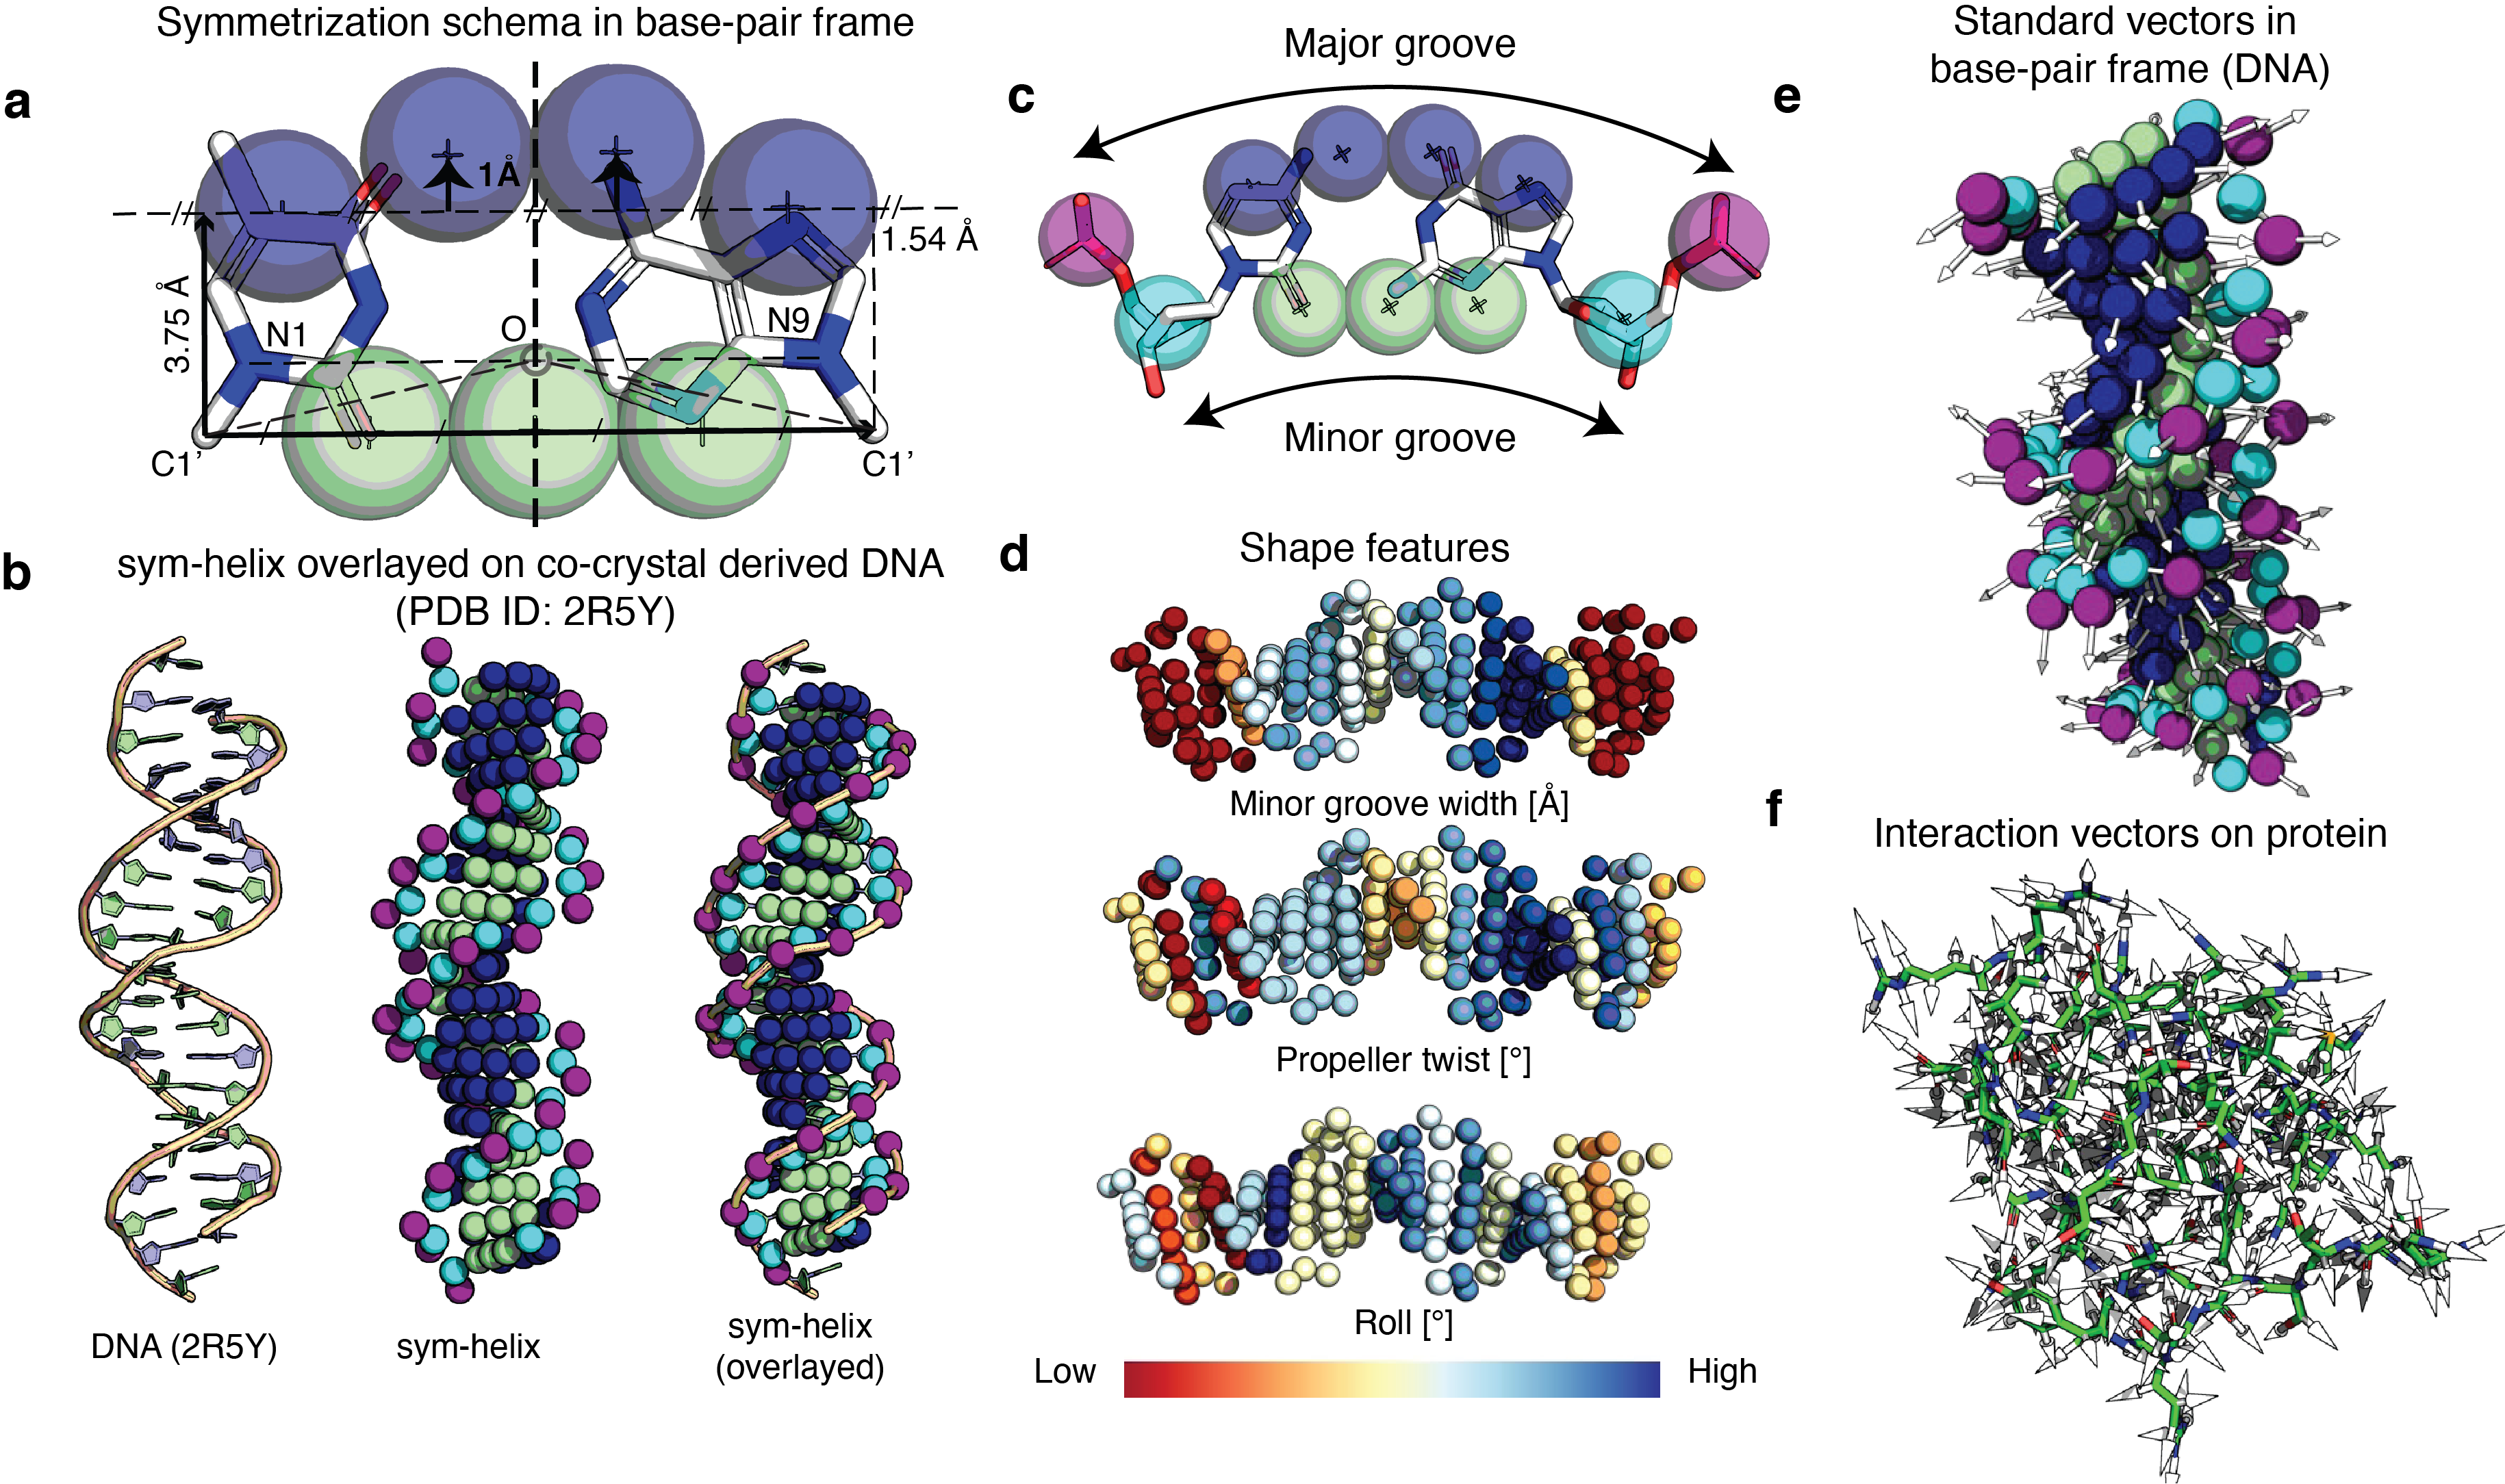
\includegraphics[width=\linewidth]{./pdnafigs/figS2.png}
 % archetecture.png: 1149x508 px, 72dpi, 40.53x17.92 cm, bb=0 0 1149 508
    \caption[Examples of continuous time prediction of ESC differentiation.]{\textbf{Examples of continuous time prediction of ESC differentiation.} Reconstruction (up to $t=6.8$) and future prediction (for $t>6.8$) for 4 example genes by a  latent ODE \citep{chen2018neural} trained on ESC data \citep{Klein2015} for 1000000 iterations, showing a good fit for the initial timepoints, but underfitting for the later timepoints.}
  \label{fig:pdnaS2}
\end{figure}
\end{center}

\begin{center}
\begin{figure}[H]
  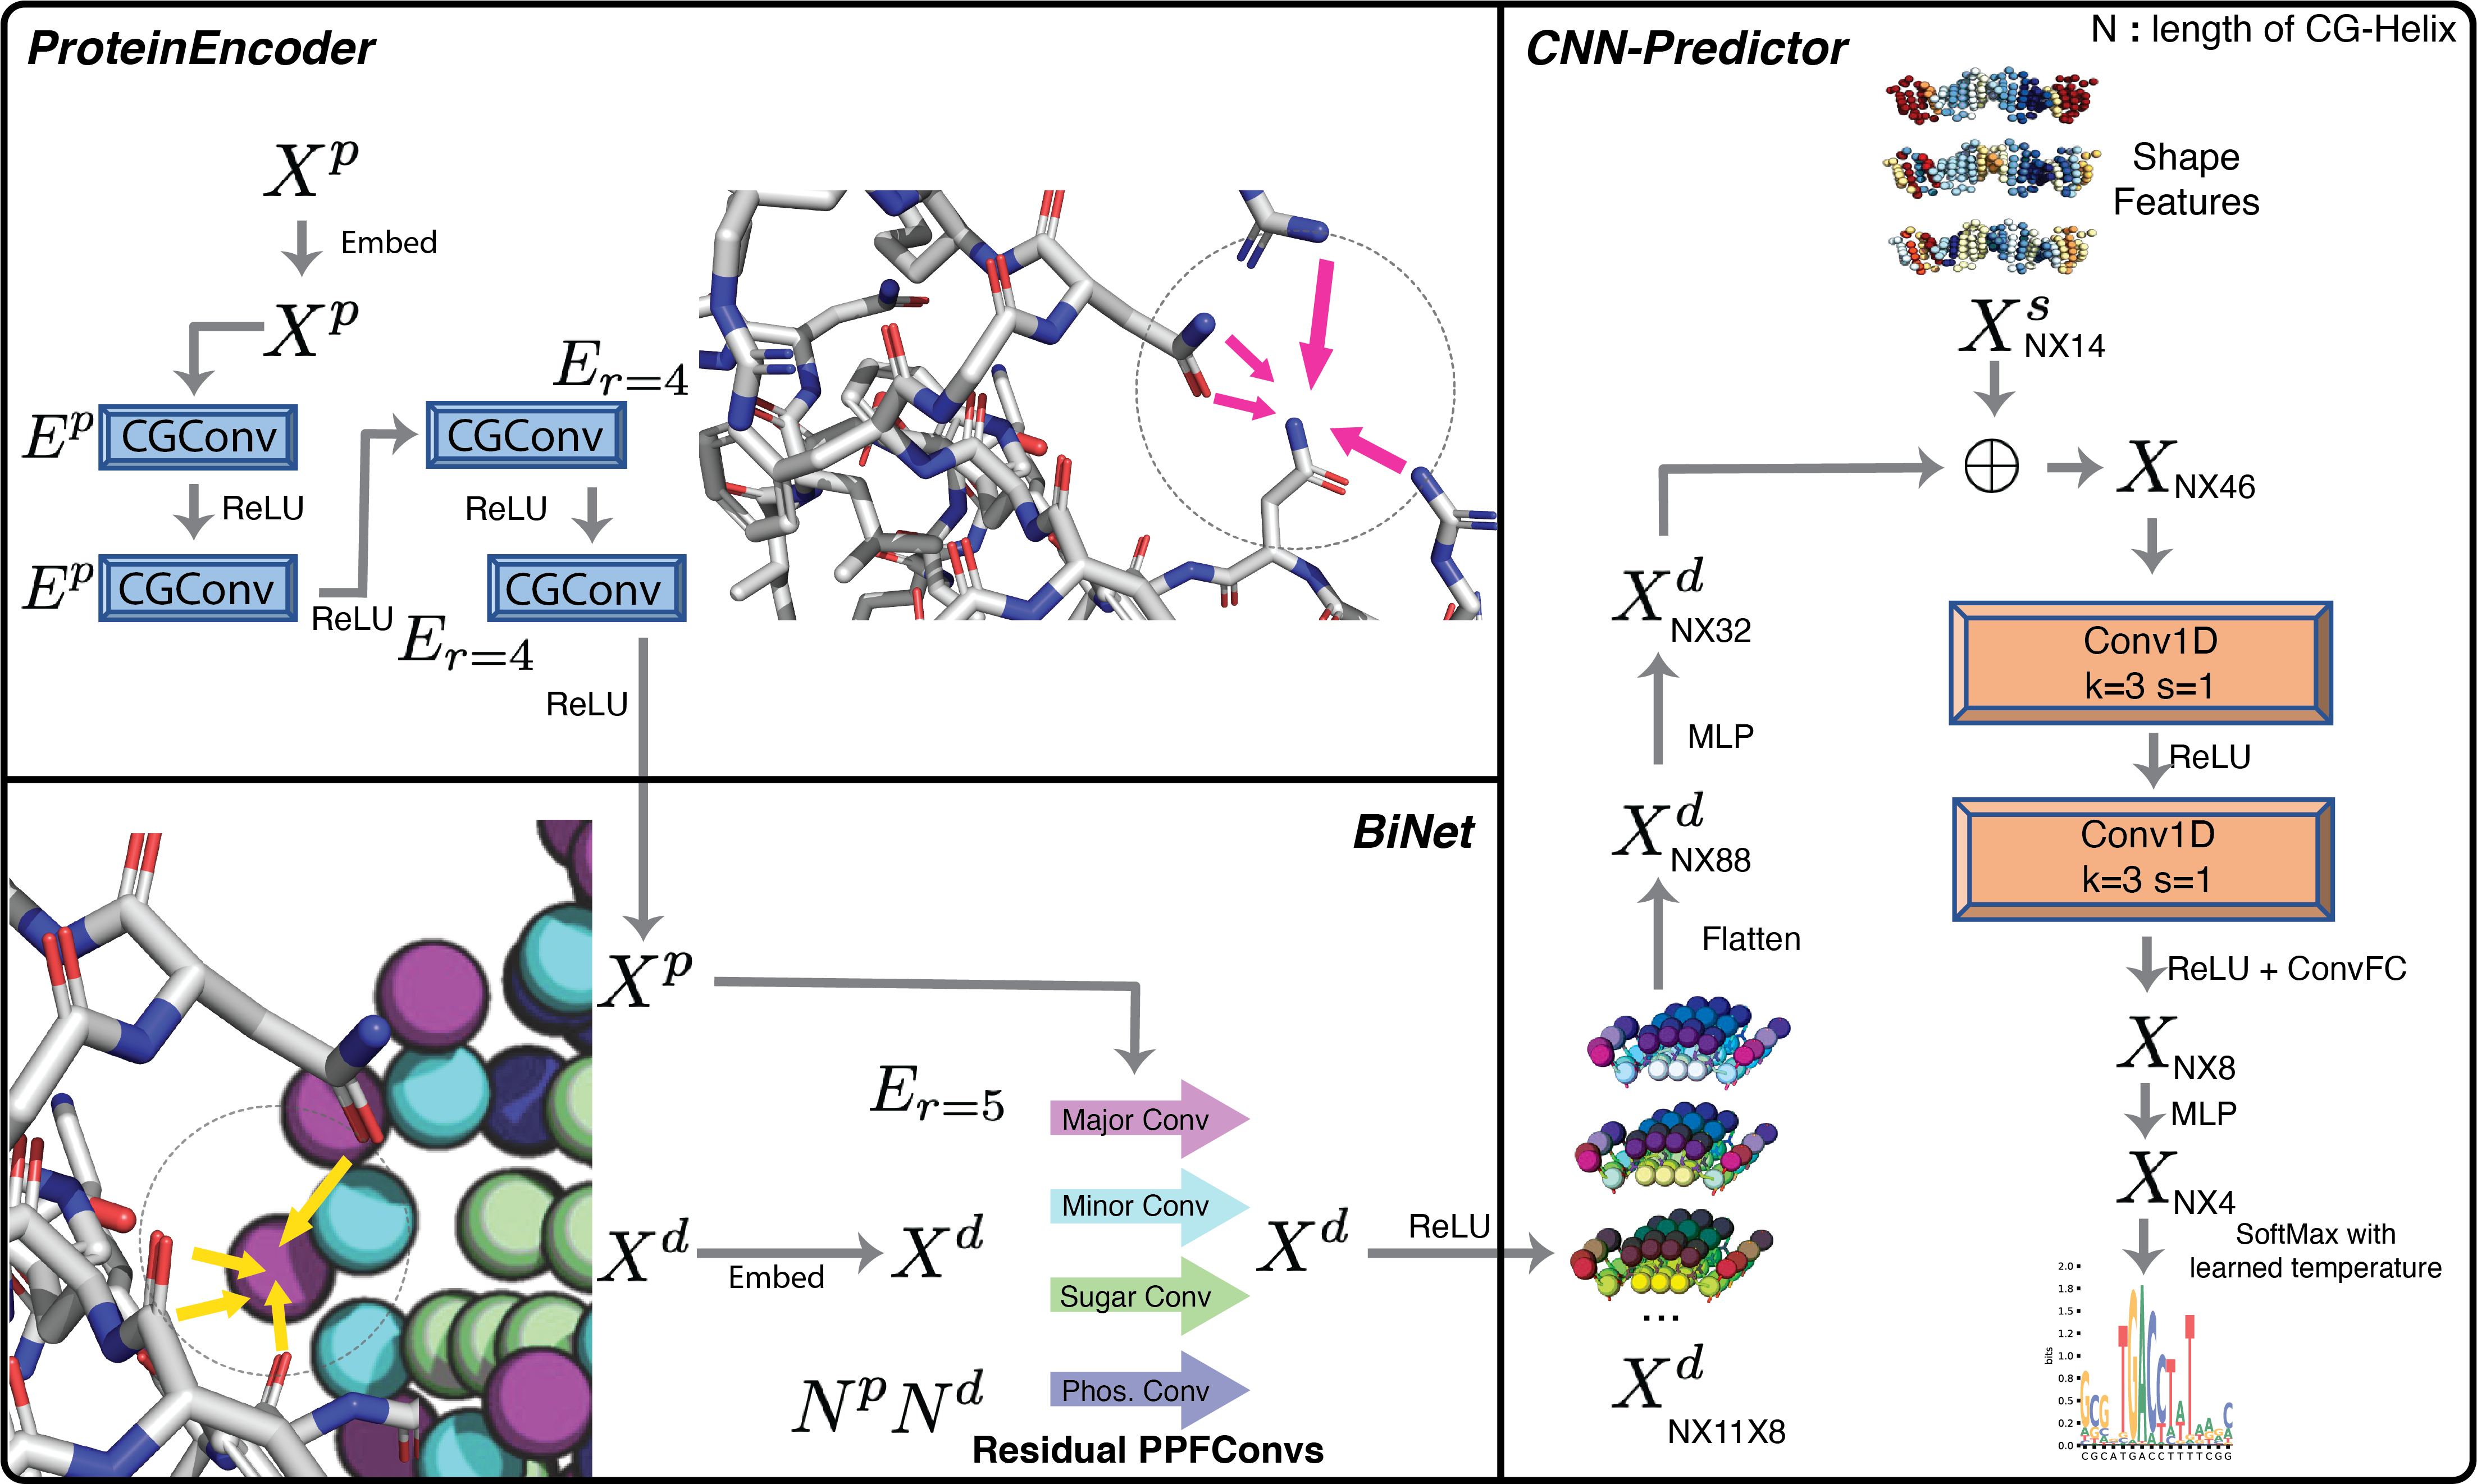
\includegraphics[width=\linewidth]{./pdnafigs/figS3.png}
 % archetecture.png: 1149x508 px, 72dpi, 40.53x17.92 cm, bb=0 0 1149 508
    \caption[Examples of continuous time prediction of ESC differentiation.]{\textbf{Examples of continuous time prediction of ESC differentiation.} Reconstruction (up to $t=6.8$) and future prediction (for $t>6.8$) for 4 example genes by a  latent ODE \citep{chen2018neural} trained on ESC data \citep{Klein2015} for 1000000 iterations, showing a good fit for the initial timepoints, but underfitting for the later timepoints.}
  \label{fig:pdnaS3}
\end{figure}
\end{center}

\begin{center}
\begin{figure}[H]
  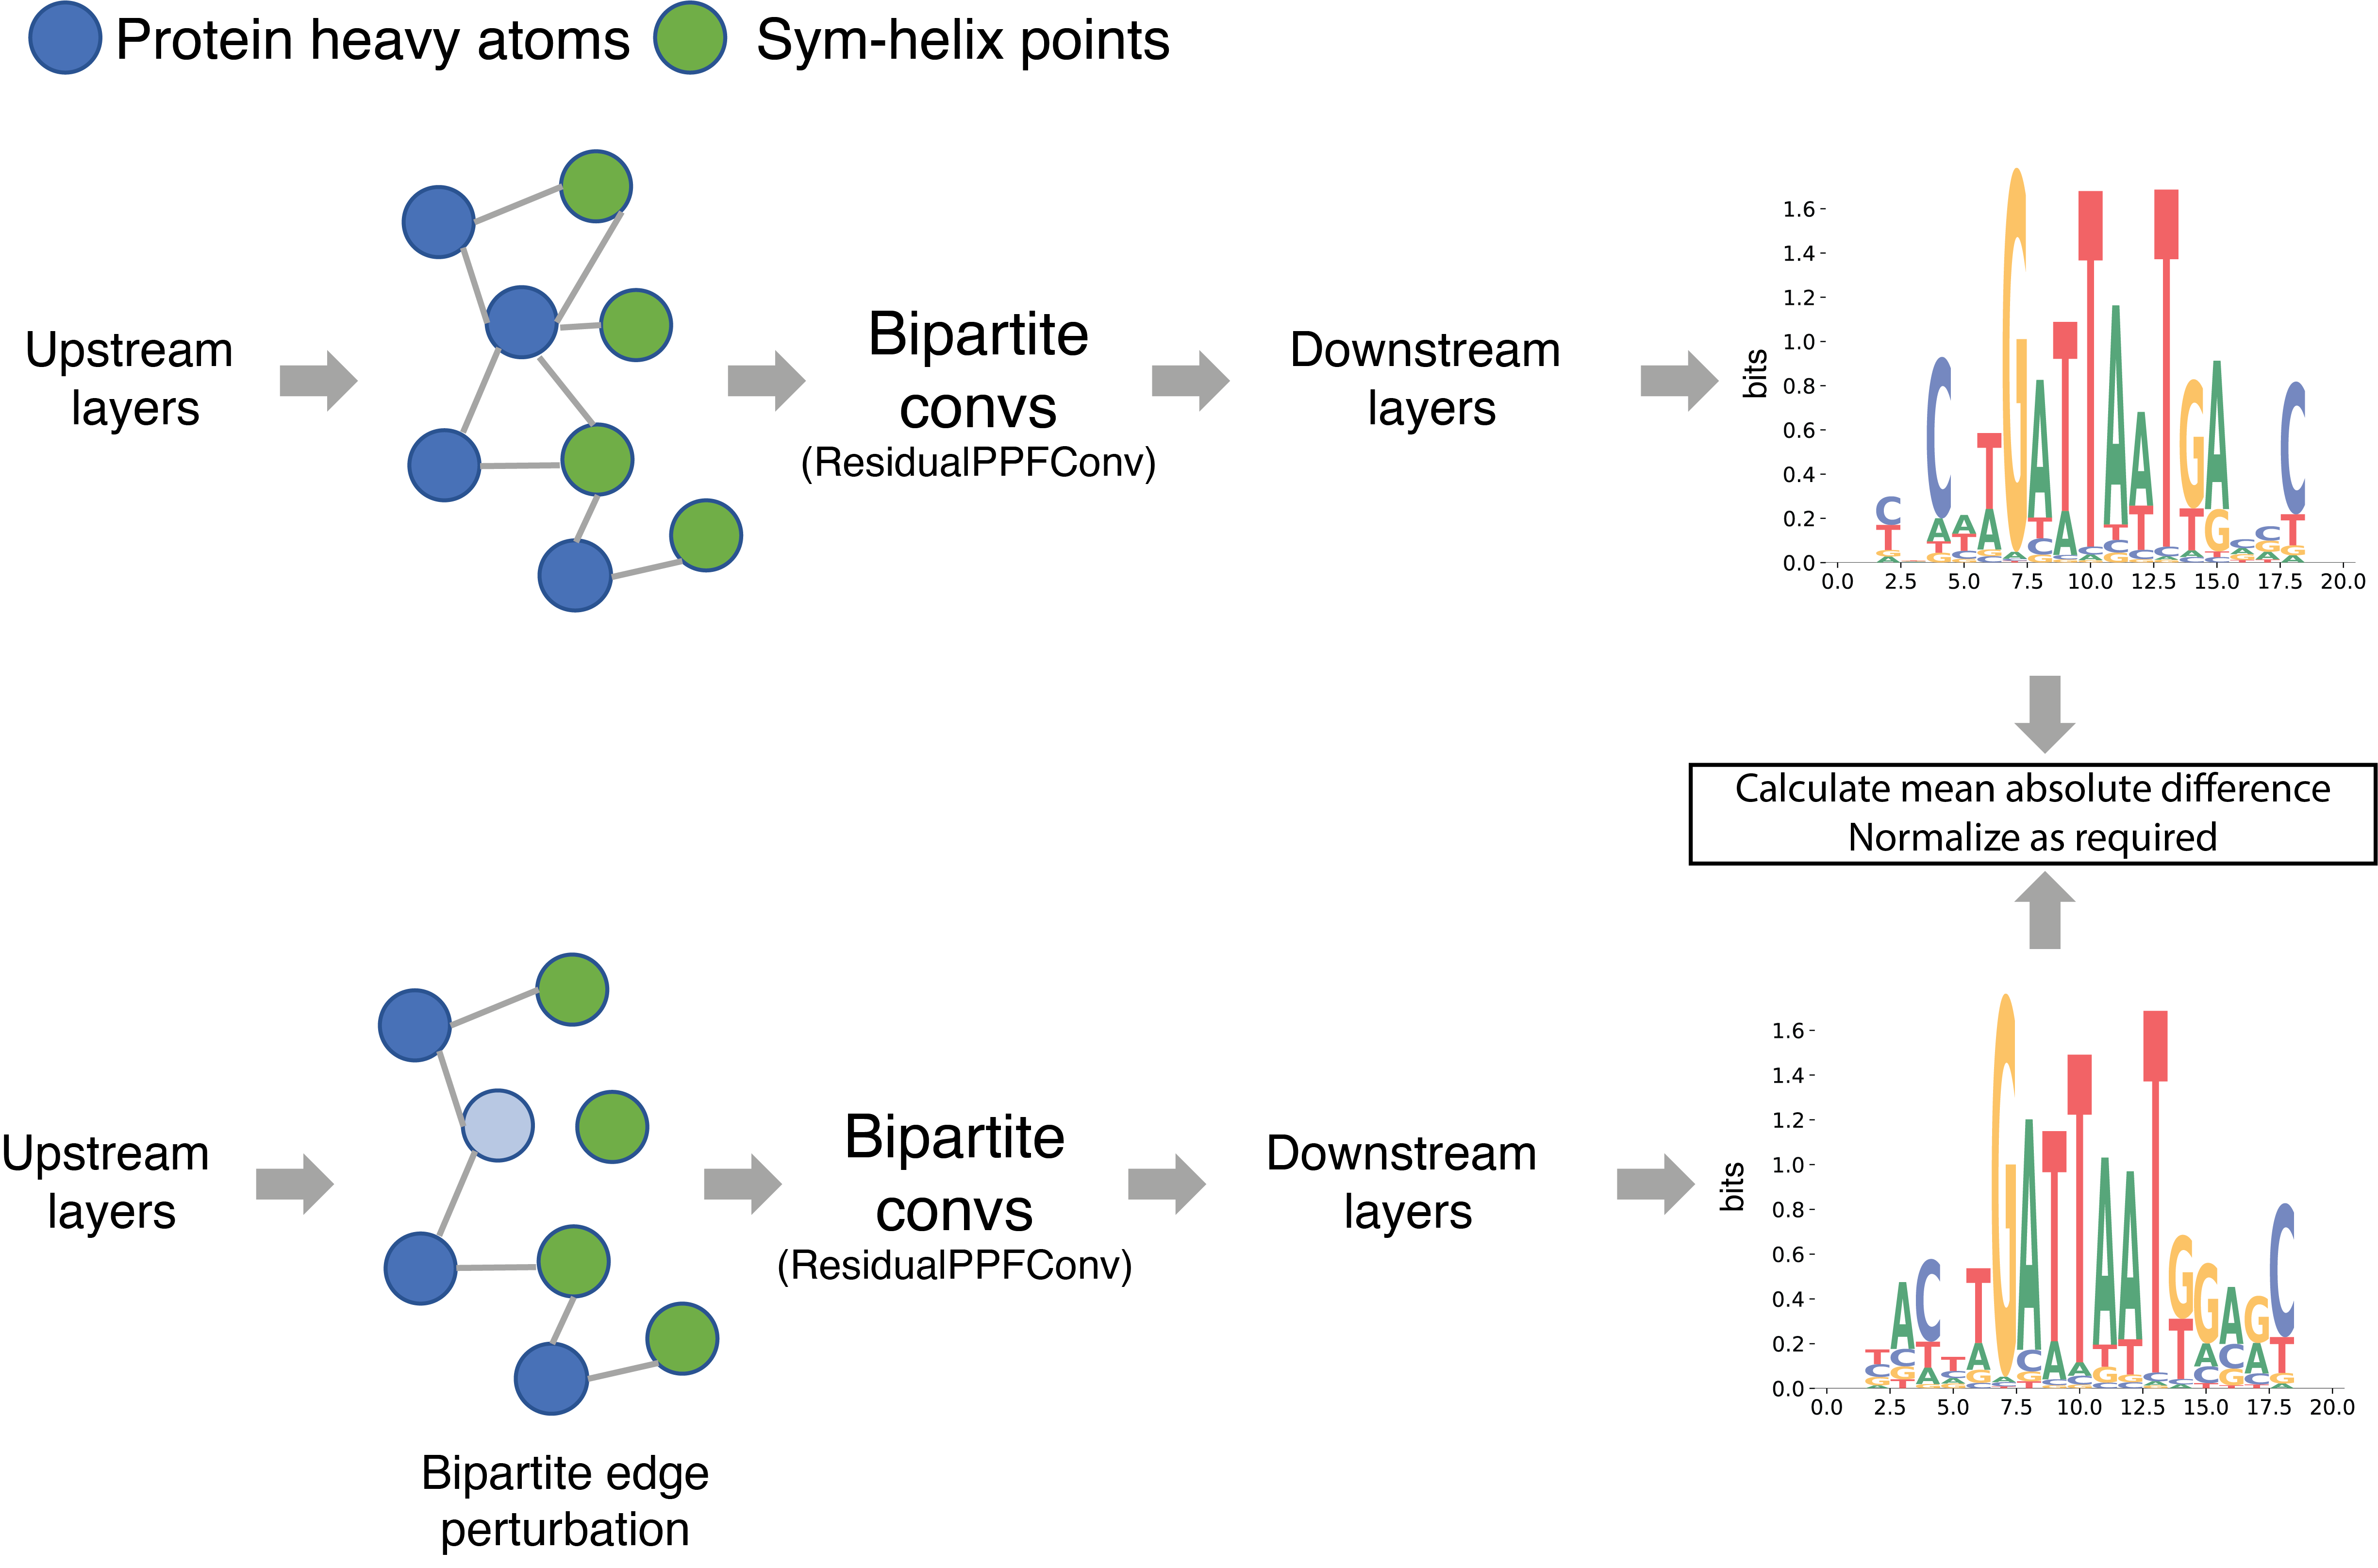
\includegraphics[width=\linewidth]{./pdnafigs/figS4.png}
 % archetecture.png: 1149x508 px, 72dpi, 40.53x17.92 cm, bb=0 0 1149 508
    \caption[Examples of continuous time prediction of ESC differentiation.]{\textbf{Examples of continuous time prediction of ESC differentiation.} Reconstruction (up to $t=6.8$) and future prediction (for $t>6.8$) for 4 example genes by a  latent ODE \citep{chen2018neural} trained on ESC data \citep{Klein2015} for 1000000 iterations, showing a good fit for the initial timepoints, but underfitting for the later timepoints.}
  \label{fig:pdnaS4}
\end{figure}
\end{center}

\begin{center}
\begin{figure}[H]
  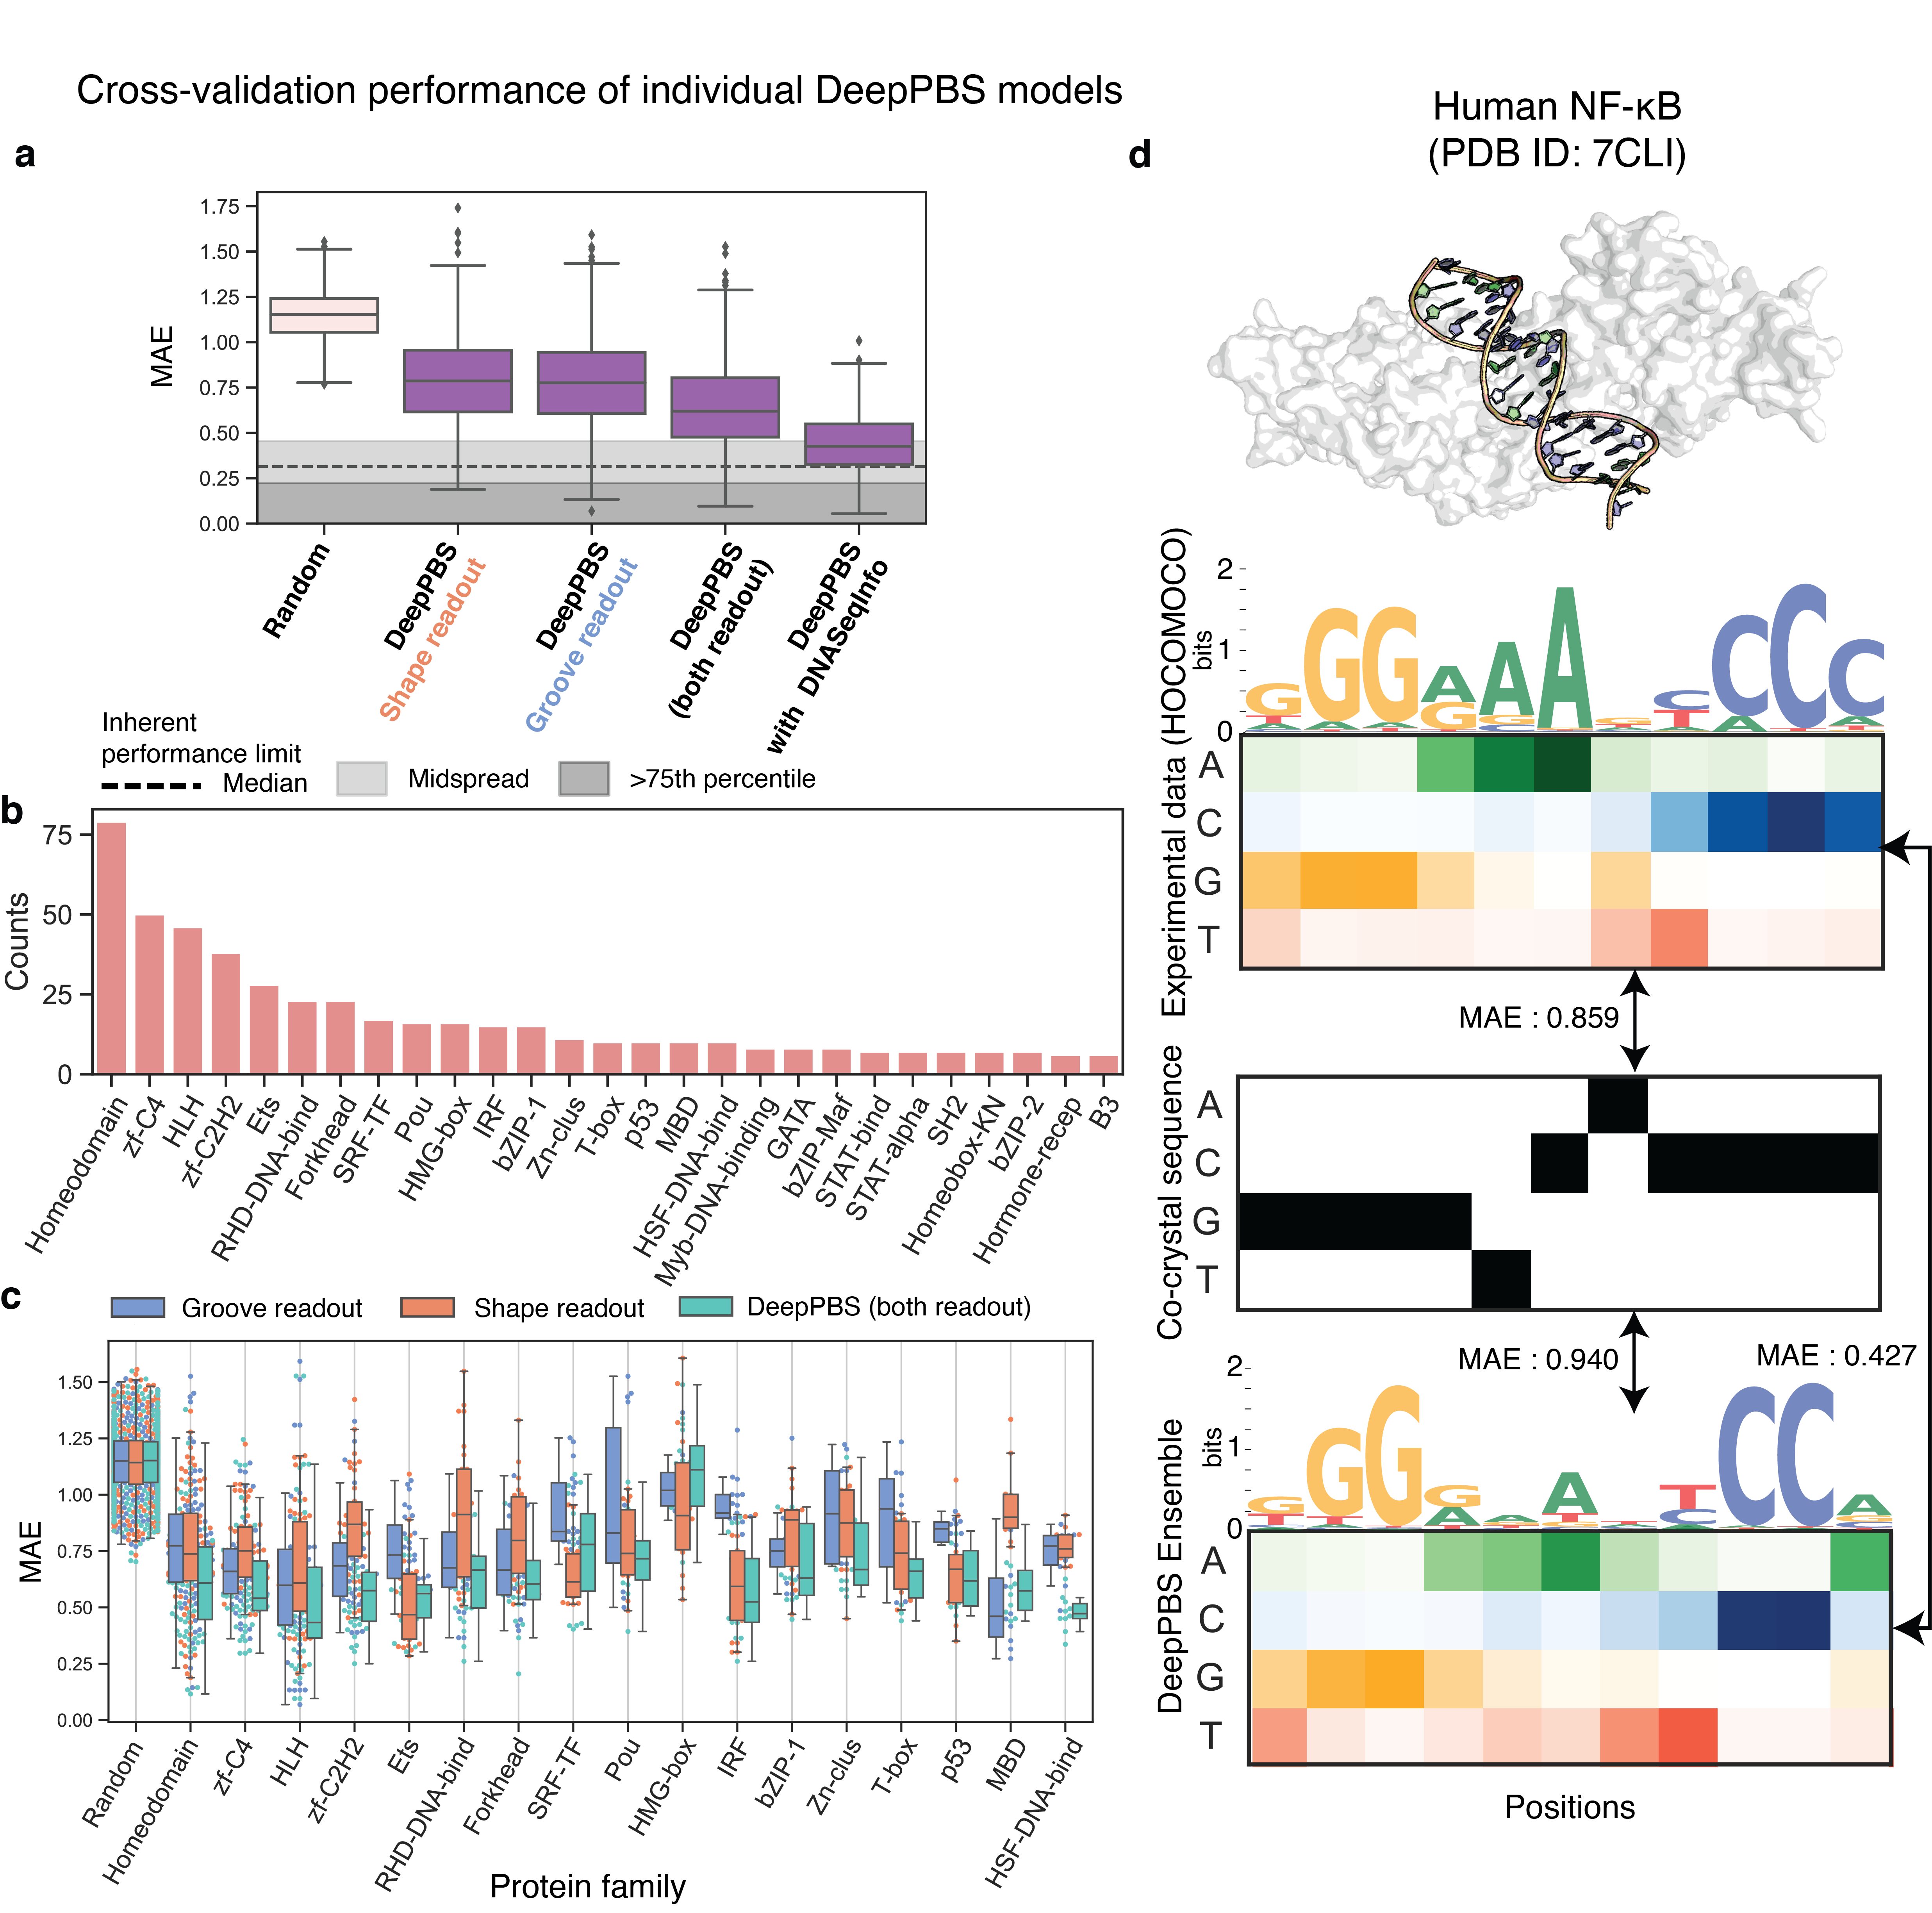
\includegraphics[width=\linewidth]{./pdnafigs/figS5.png}
 % archetecture.png: 1149x508 px, 72dpi, 40.53x17.92 cm, bb=0 0 1149 508
    \caption[Examples of continuous time prediction of ESC differentiation.]{\textbf{Examples of continuous time prediction of ESC differentiation.} Reconstruction (up to $t=6.8$) and future prediction (for $t>6.8$) for 4 example genes by a  latent ODE \citep{chen2018neural} trained on ESC data \citep{Klein2015} for 1000000 iterations, showing a good fit for the initial timepoints, but underfitting for the later timepoints.}
  \label{fig:pdnaS5}
\end{figure}
\end{center}

\begin{center}
\begin{figure}[H]
  \includegraphics[width=\linewidth]{./pdnafigs/figS6.png}
 % archetecture.png: 1149x508 px, 72dpi, 40.53x17.92 cm, bb=0 0 1149 508
    \caption[Examples of continuous time prediction of ESC differentiation.]{\textbf{Examples of continuous time prediction of ESC differentiation.} Reconstruction (up to $t=6.8$) and future prediction (for $t>6.8$) for 4 example genes by a  latent ODE \citep{chen2018neural} trained on ESC data \citep{Klein2015} for 1000000 iterations, showing a good fit for the initial timepoints, but underfitting for the later timepoints.}
  \label{fig:pdnaS6}
\end{figure}
\end{center}

\begin{center}
\begin{figure}[H]
  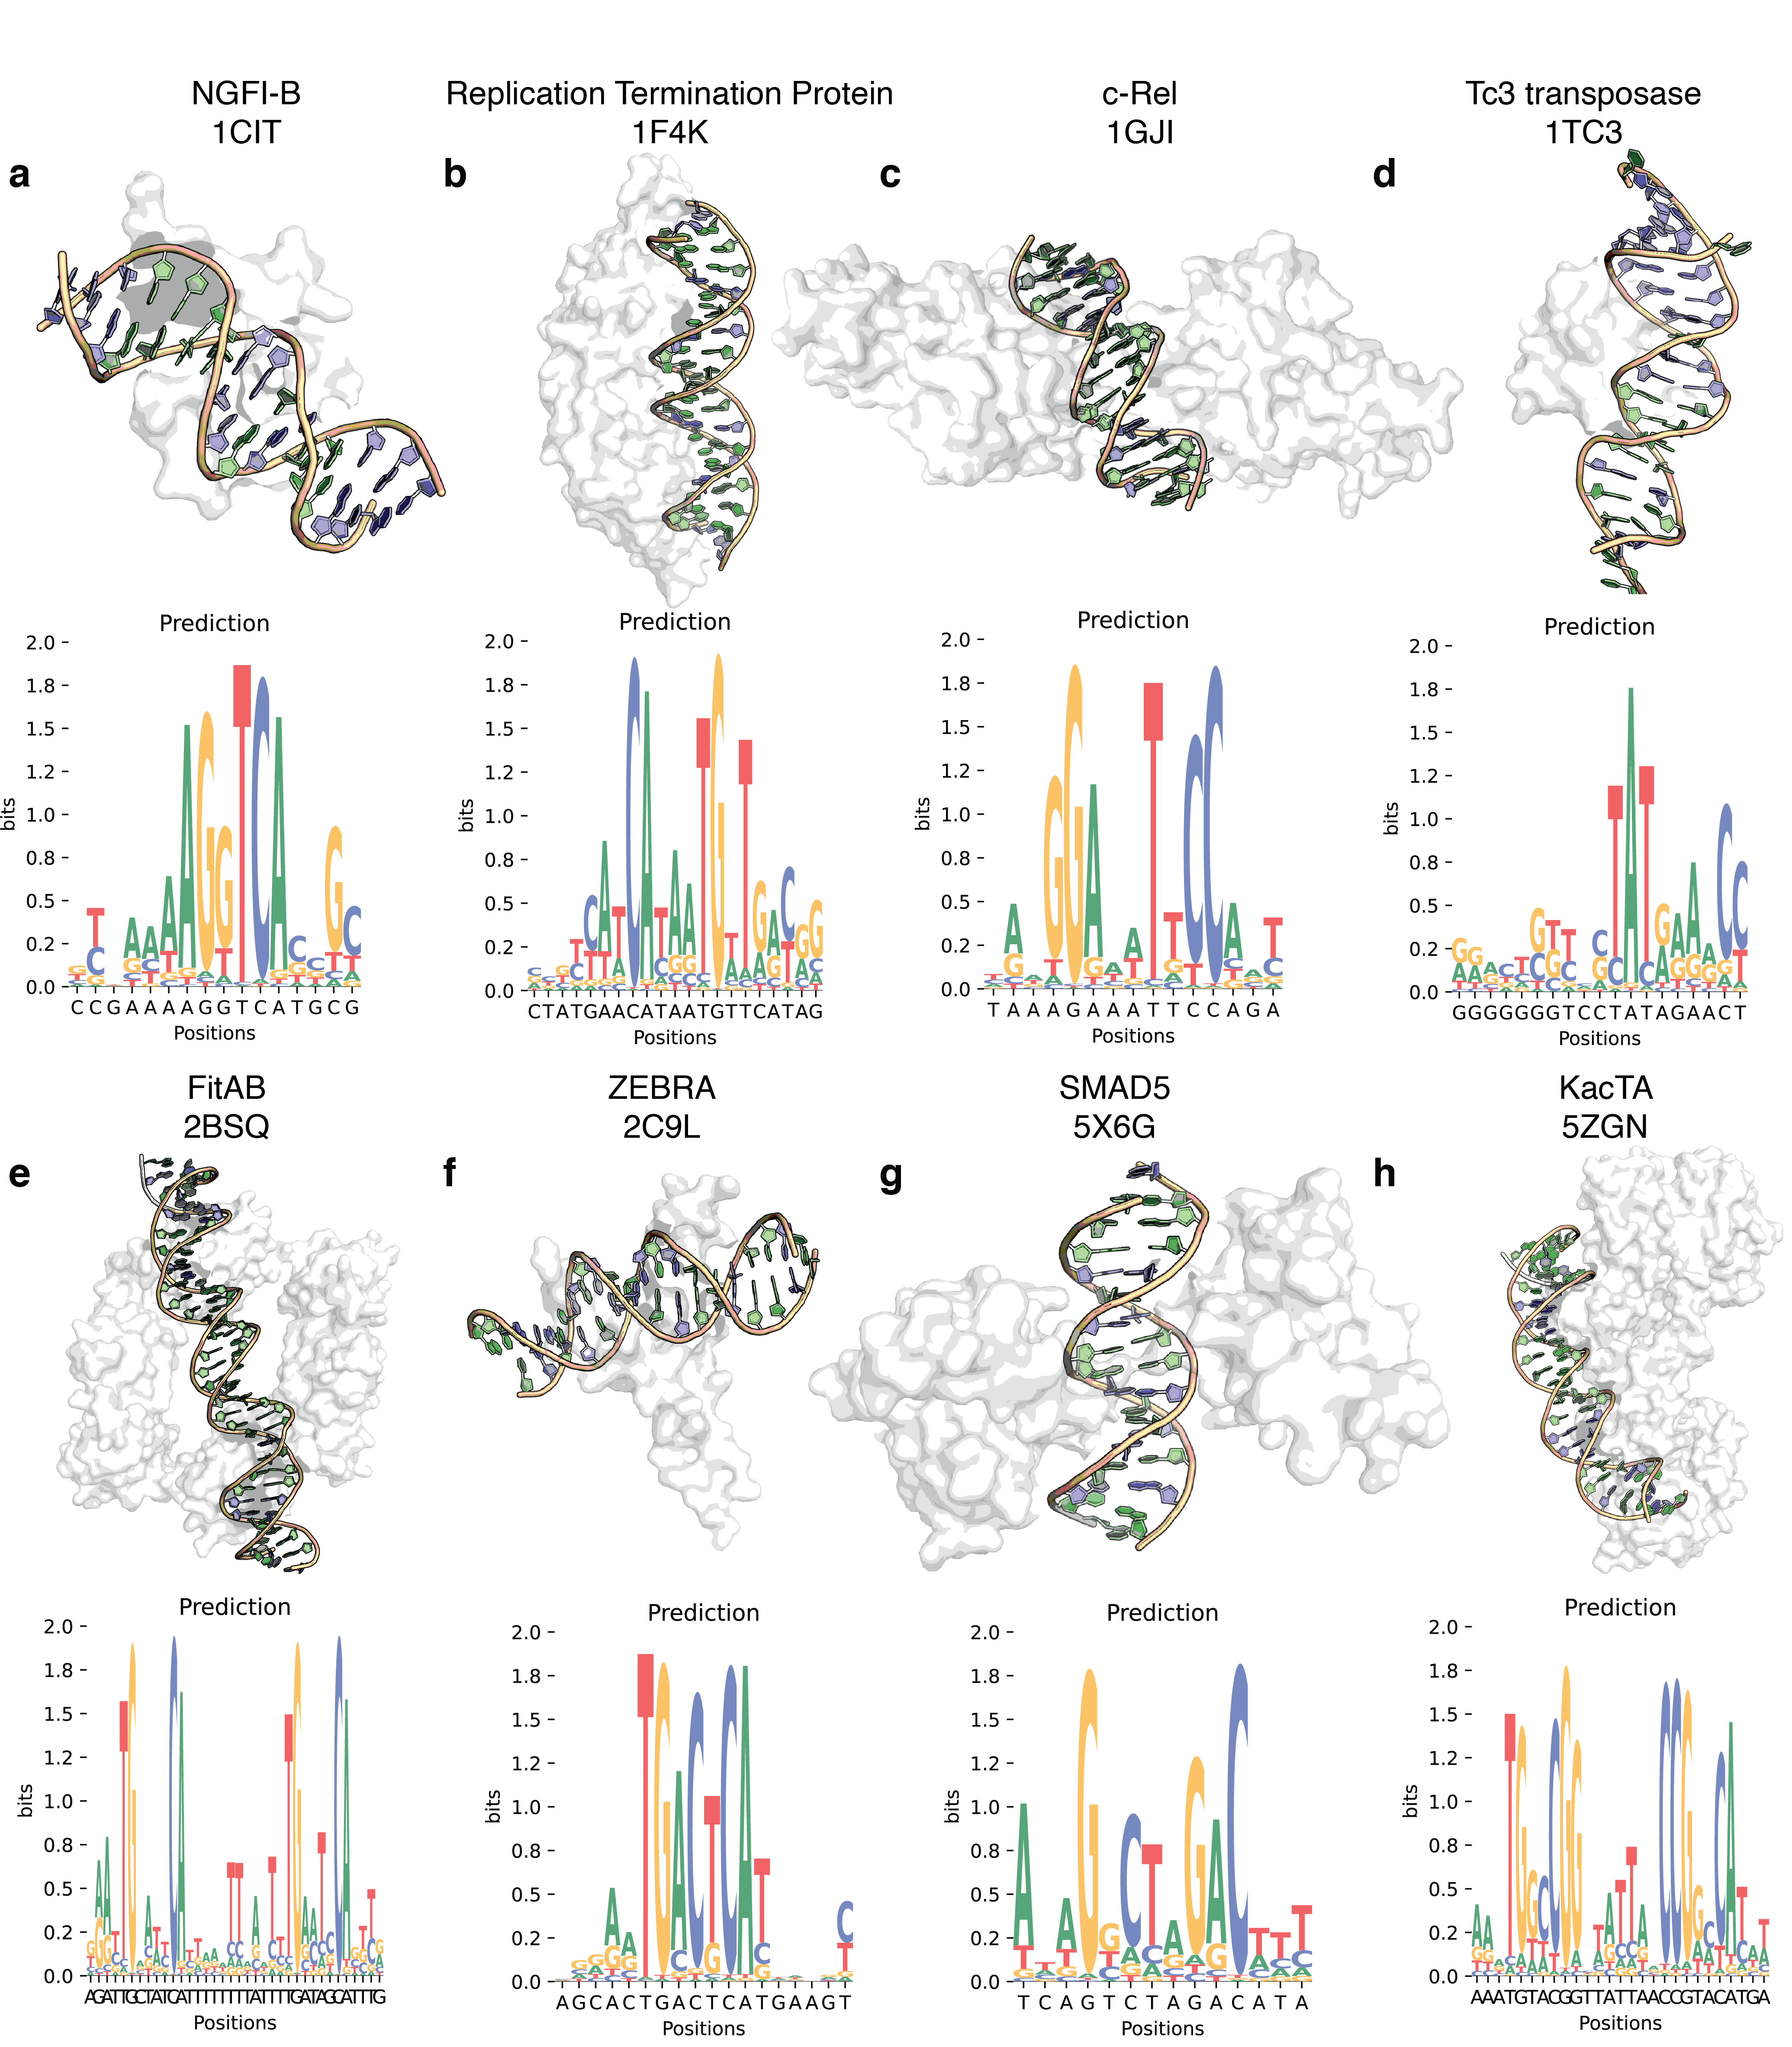
\includegraphics[width=\linewidth]{./pdnafigs/figS7.png}
 % archetecture.png: 1149x508 px, 72dpi, 40.53x17.92 cm, bb=0 0 1149 508
    \caption[Examples of continuous time prediction of ESC differentiation.]{\textbf{Examples of continuous time prediction of ESC differentiation.} Reconstruction (up to $t=6.8$) and future prediction (for $t>6.8$) for 4 example genes by a  latent ODE \citep{chen2018neural} trained on ESC data \citep{Klein2015} for 1000000 iterations, showing a good fit for the initial timepoints, but underfitting for the later timepoints.}
  \label{fig:pdnaS7}
\end{figure}
\end{center}

\begin{center}
\begin{figure}[H]
  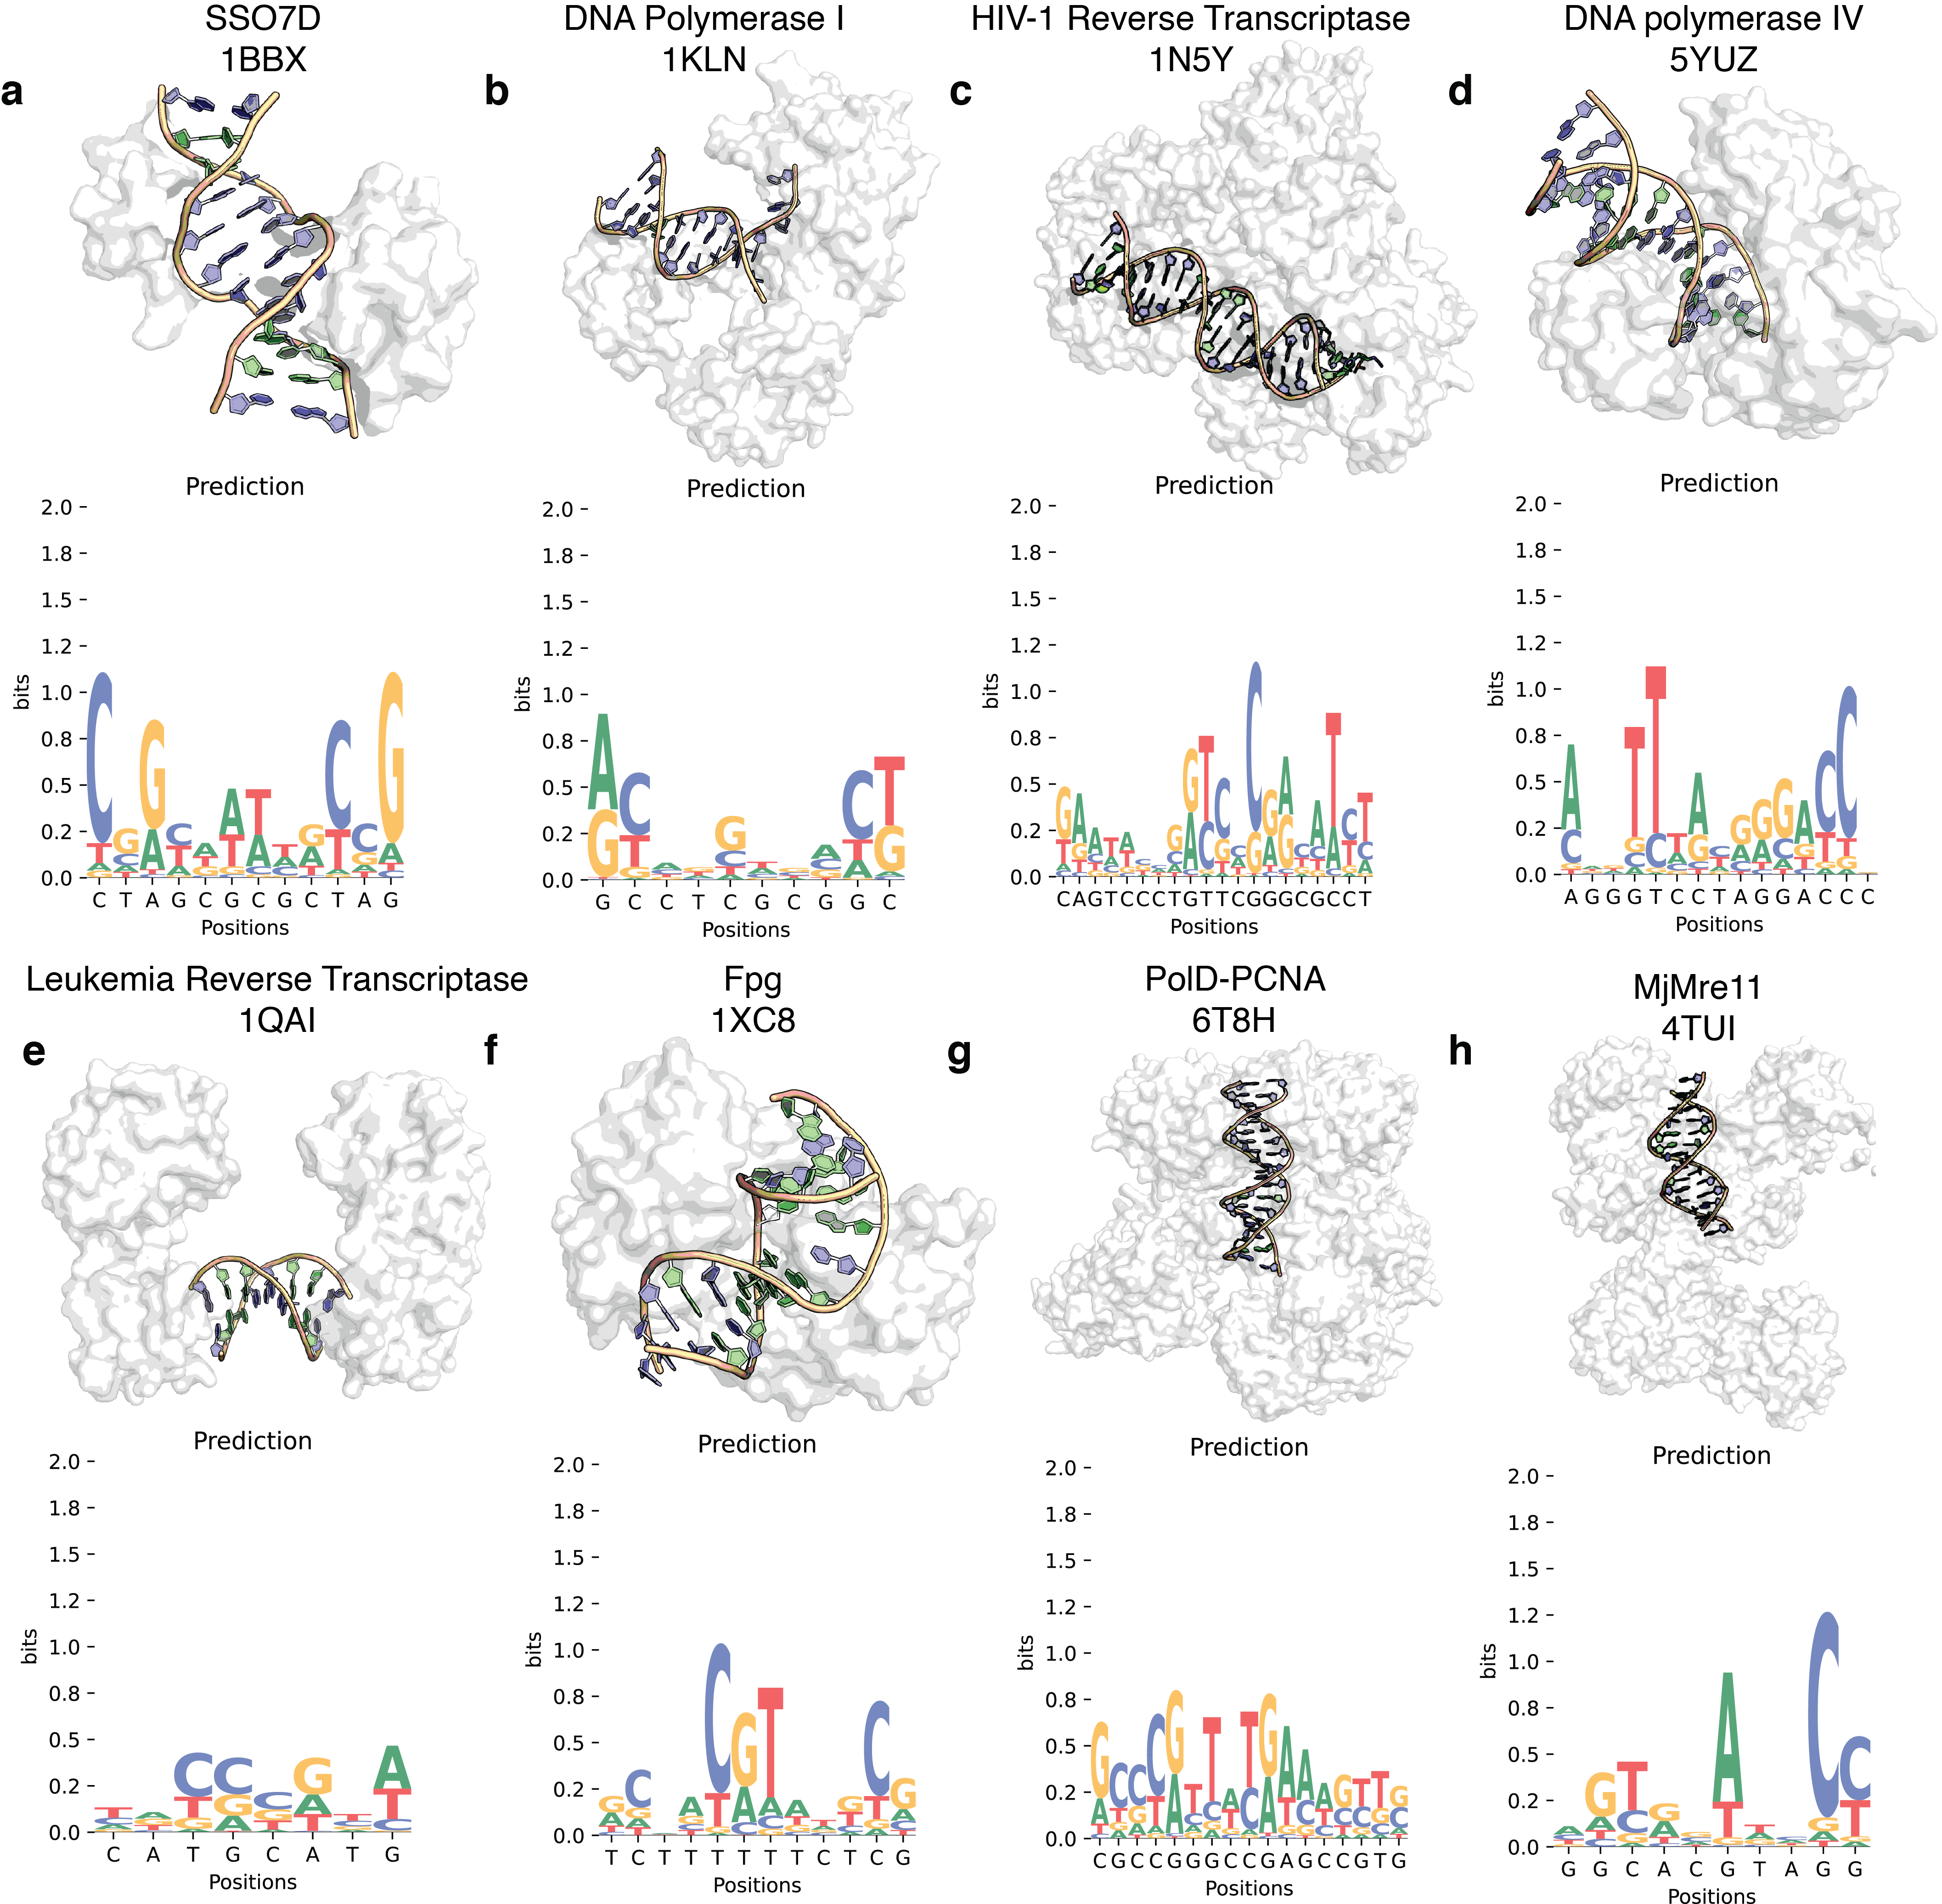
\includegraphics[width=\linewidth]{./pdnafigs/figS8.png}
 % archetecture.png: 1149x508 px, 72dpi, 40.53x17.92 cm, bb=0 0 1149 508
    \caption[Examples of continuous time prediction of ESC differentiation.]{\textbf{Examples of continuous time prediction of ESC differentiation.} Reconstruction (up to $t=6.8$) and future prediction (for $t>6.8$) for 4 example genes by a  latent ODE \citep{chen2018neural} trained on ESC data \citep{Klein2015} for 1000000 iterations, showing a good fit for the initial timepoints, but underfitting for the later timepoints.}
  \label{fig:pdnaS8}
\end{figure}
\end{center}

\begin{center}
\begin{figure}[H]
  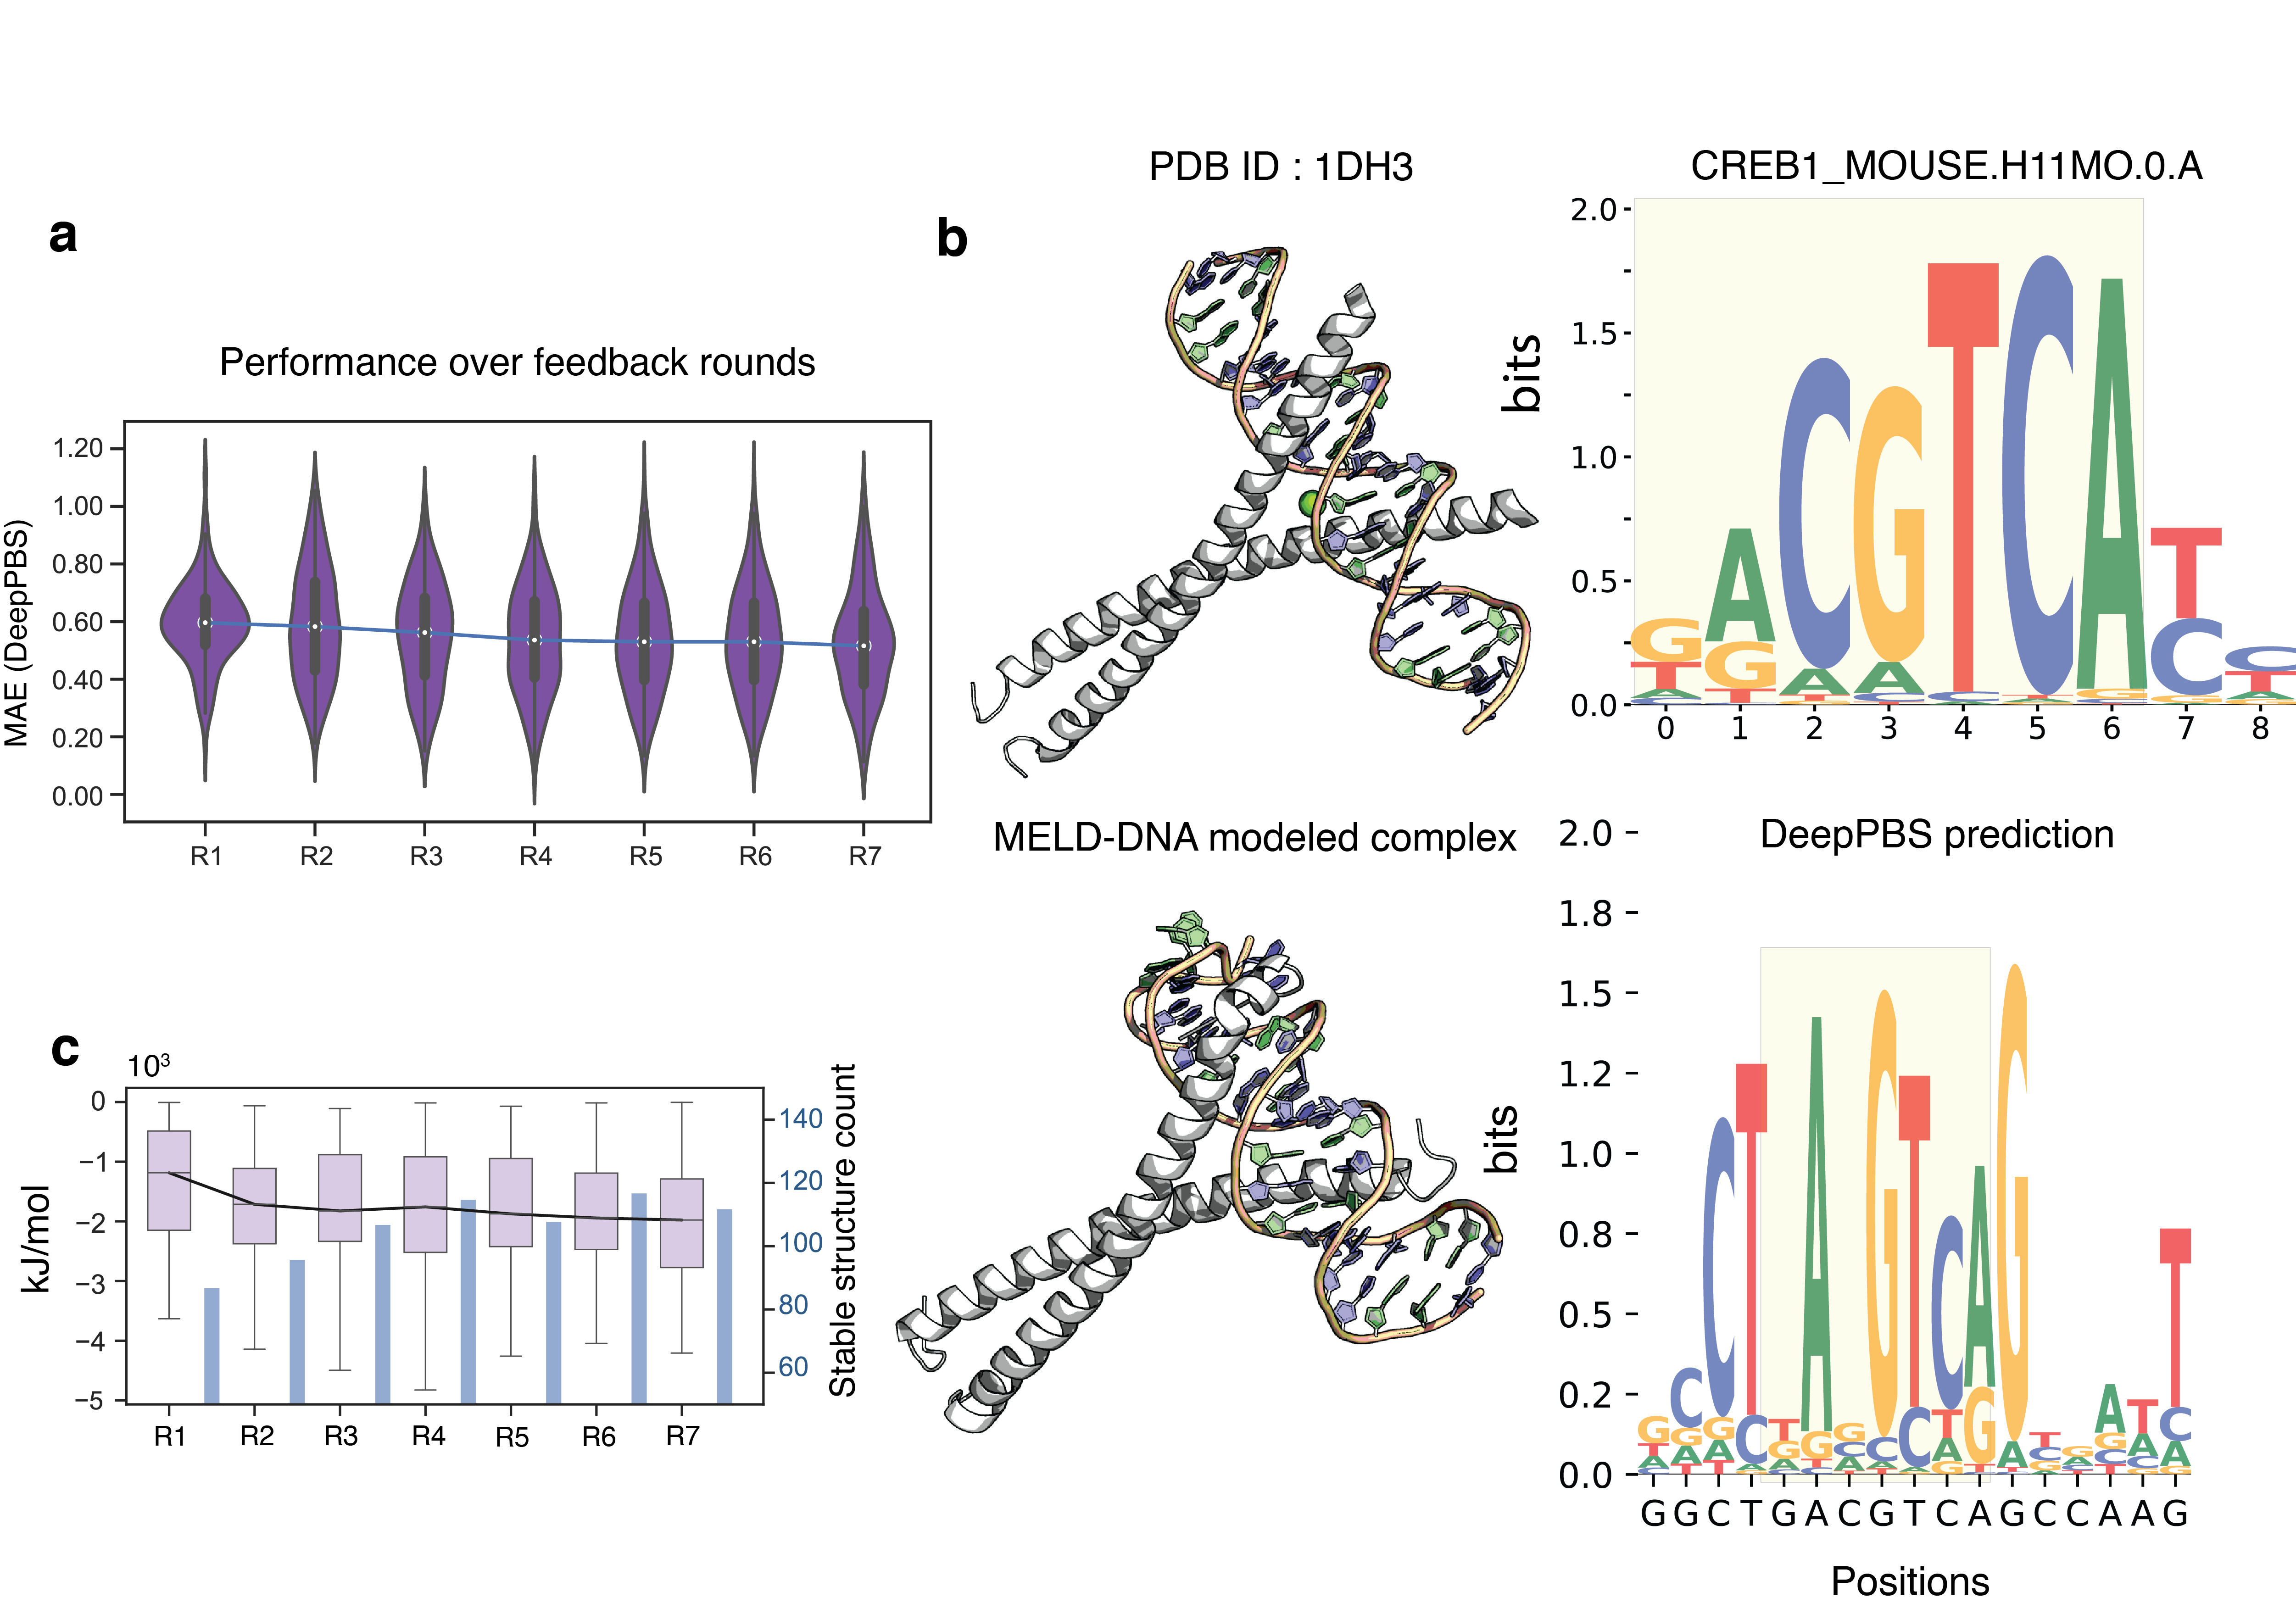
\includegraphics[width=\linewidth]{./pdnafigs/figS9.png}
 % archetecture.png: 1149x508 px, 72dpi, 40.53x17.92 cm, bb=0 0 1149 508
    \caption[Examples of continuous time prediction of ESC differentiation.]{\textbf{Examples of continuous time prediction of ESC differentiation.} Reconstruction (up to $t=6.8$) and future prediction (for $t>6.8$) for 4 example genes by a  latent ODE \citep{chen2018neural} trained on ESC data \citep{Klein2015} for 1000000 iterations, showing a good fit for the initial timepoints, but underfitting for the later timepoints.}
  \label{fig:pdnaS9}
\end{figure}
\end{center}

\begin{center}
\begin{figure}[H]
  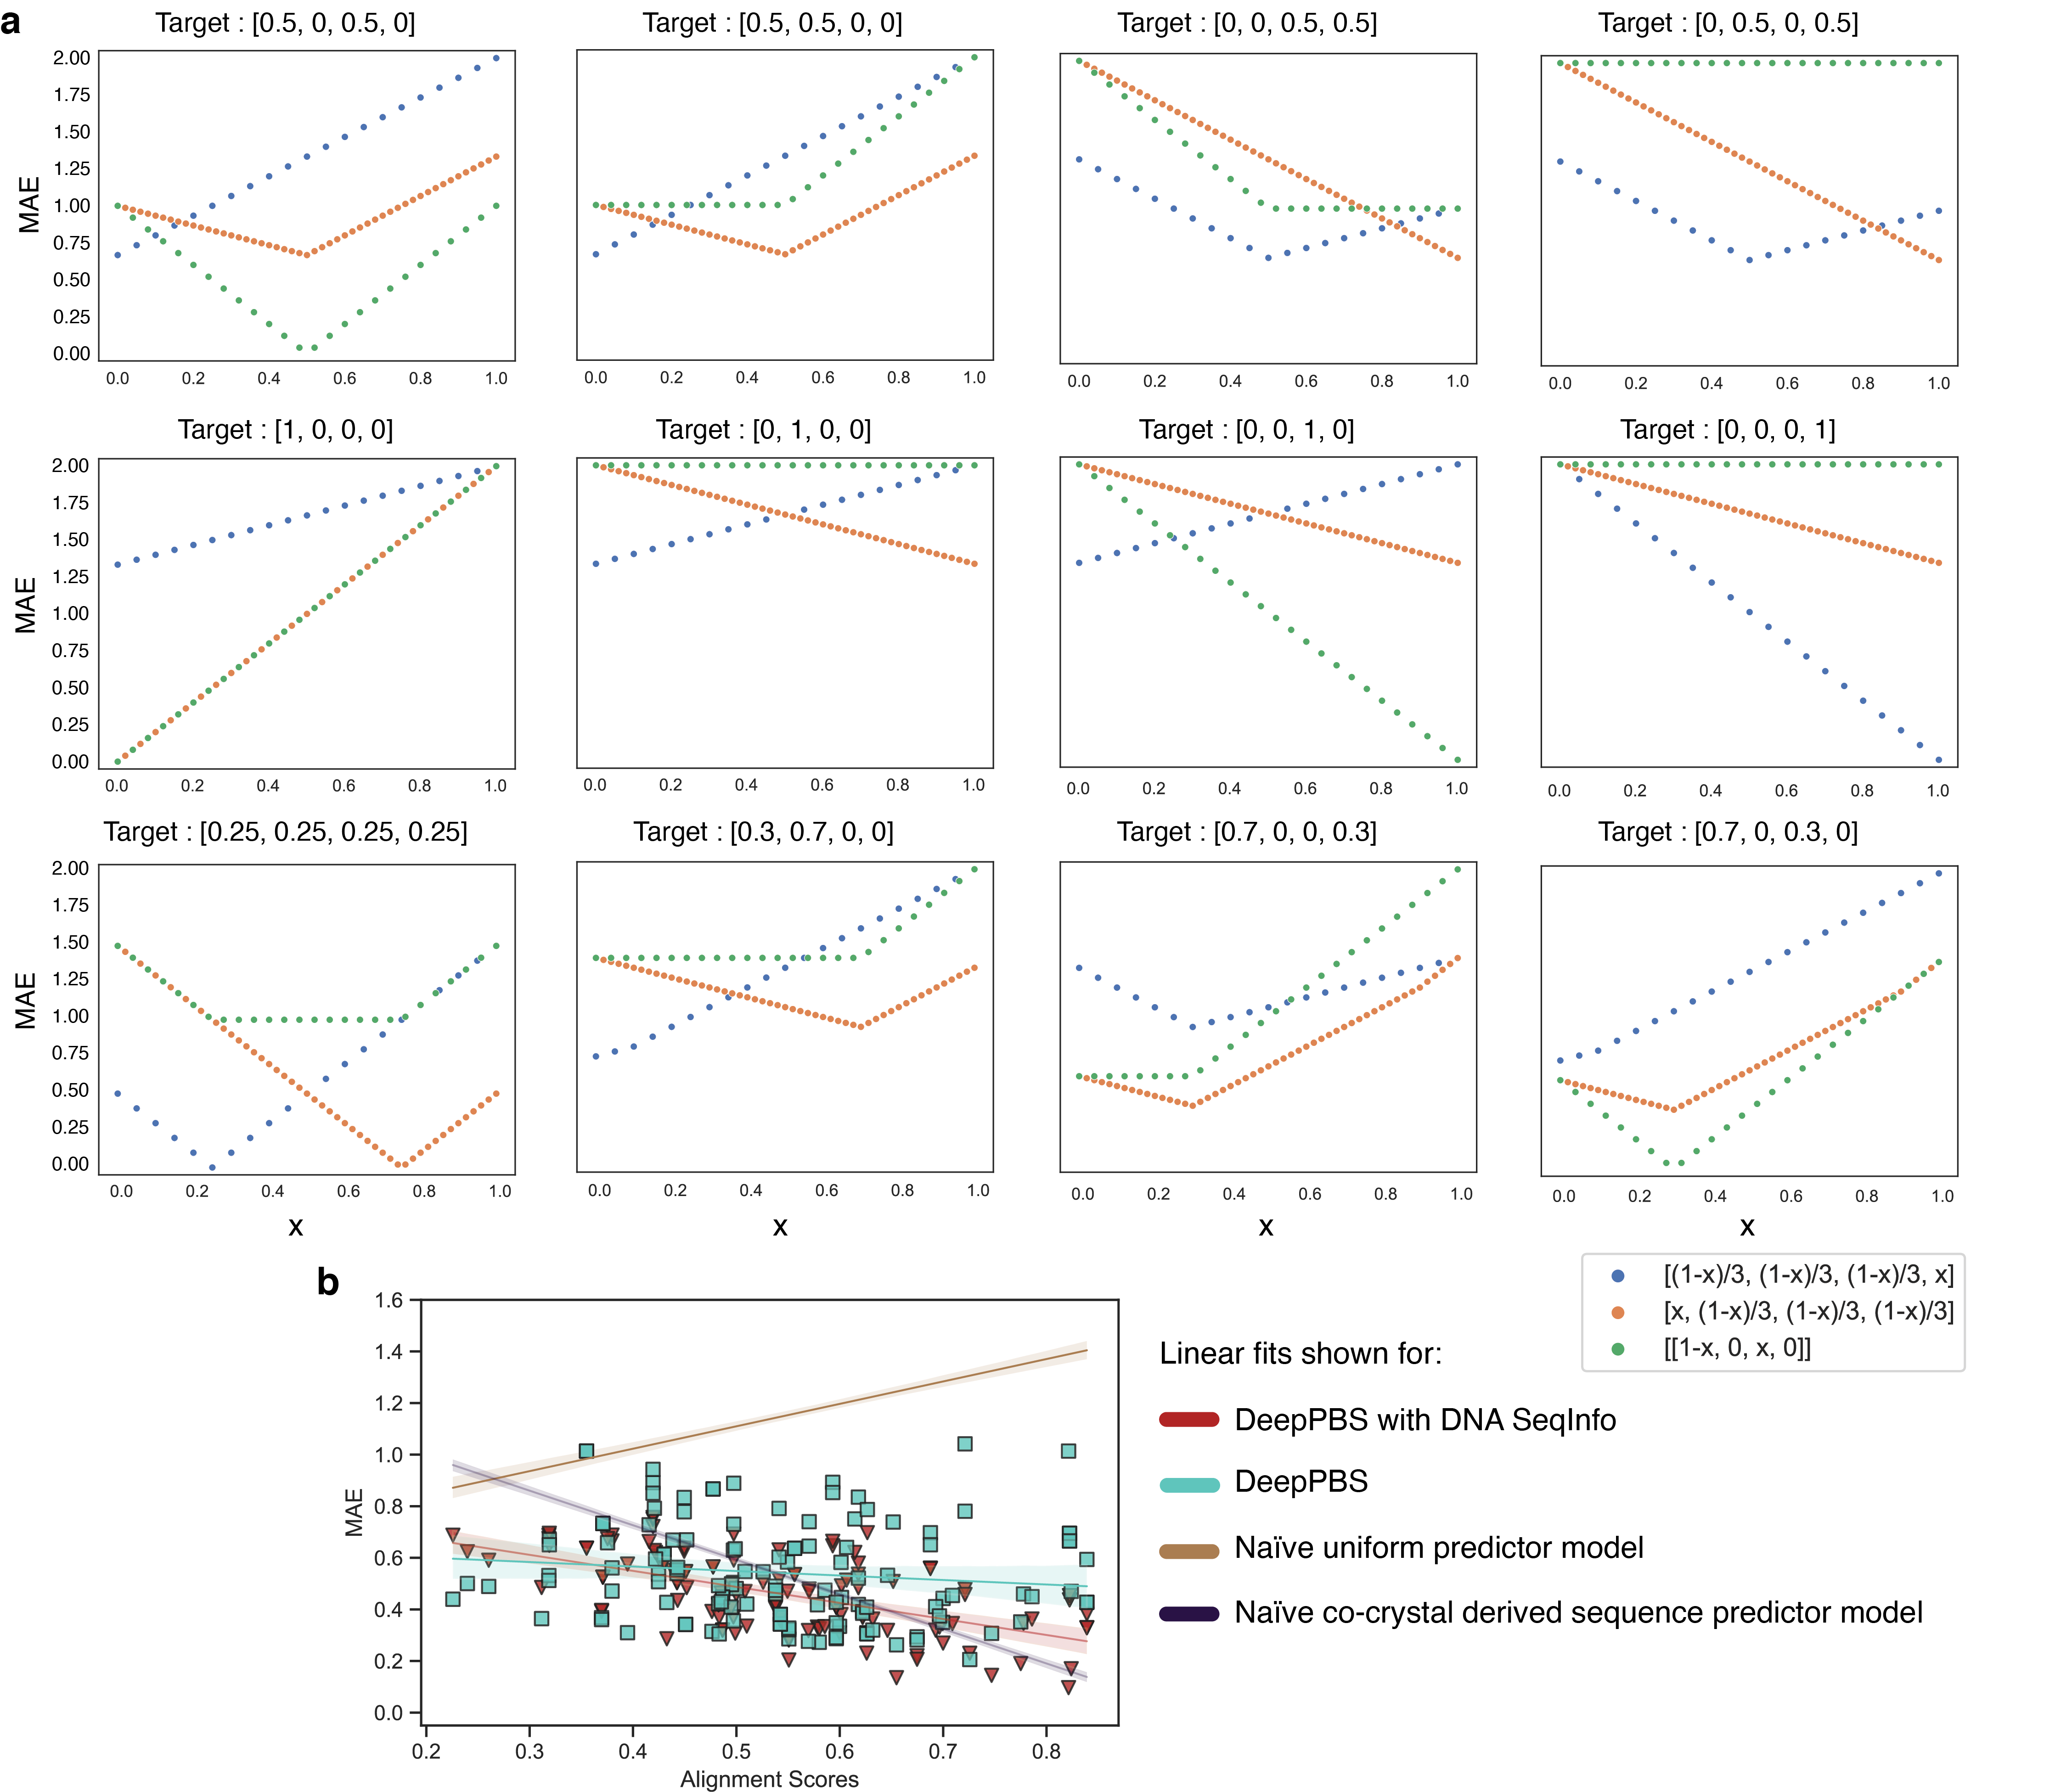
\includegraphics[width=\linewidth]{./pdnafigs/figS10.png}
 % archetecture.png: 1149x508 px, 72dpi, 40.53x17.92 cm, bb=0 0 1149 508
    \caption[Examples of continuous time prediction of ESC differentiation.]{\textbf{Examples of continuous time prediction of ESC differentiation.} Reconstruction (up to $t=6.8$) and future prediction (for $t>6.8$) for 4 example genes by a  latent ODE \citep{chen2018neural} trained on ESC data \citep{Klein2015} for 1000000 iterations, showing a good fit for the initial timepoints, but underfitting for the later timepoints.}
  \label{fig:pdnaS10}
\end{figure}
\end{center}

\begin{center}
\begin{figure}[H]
  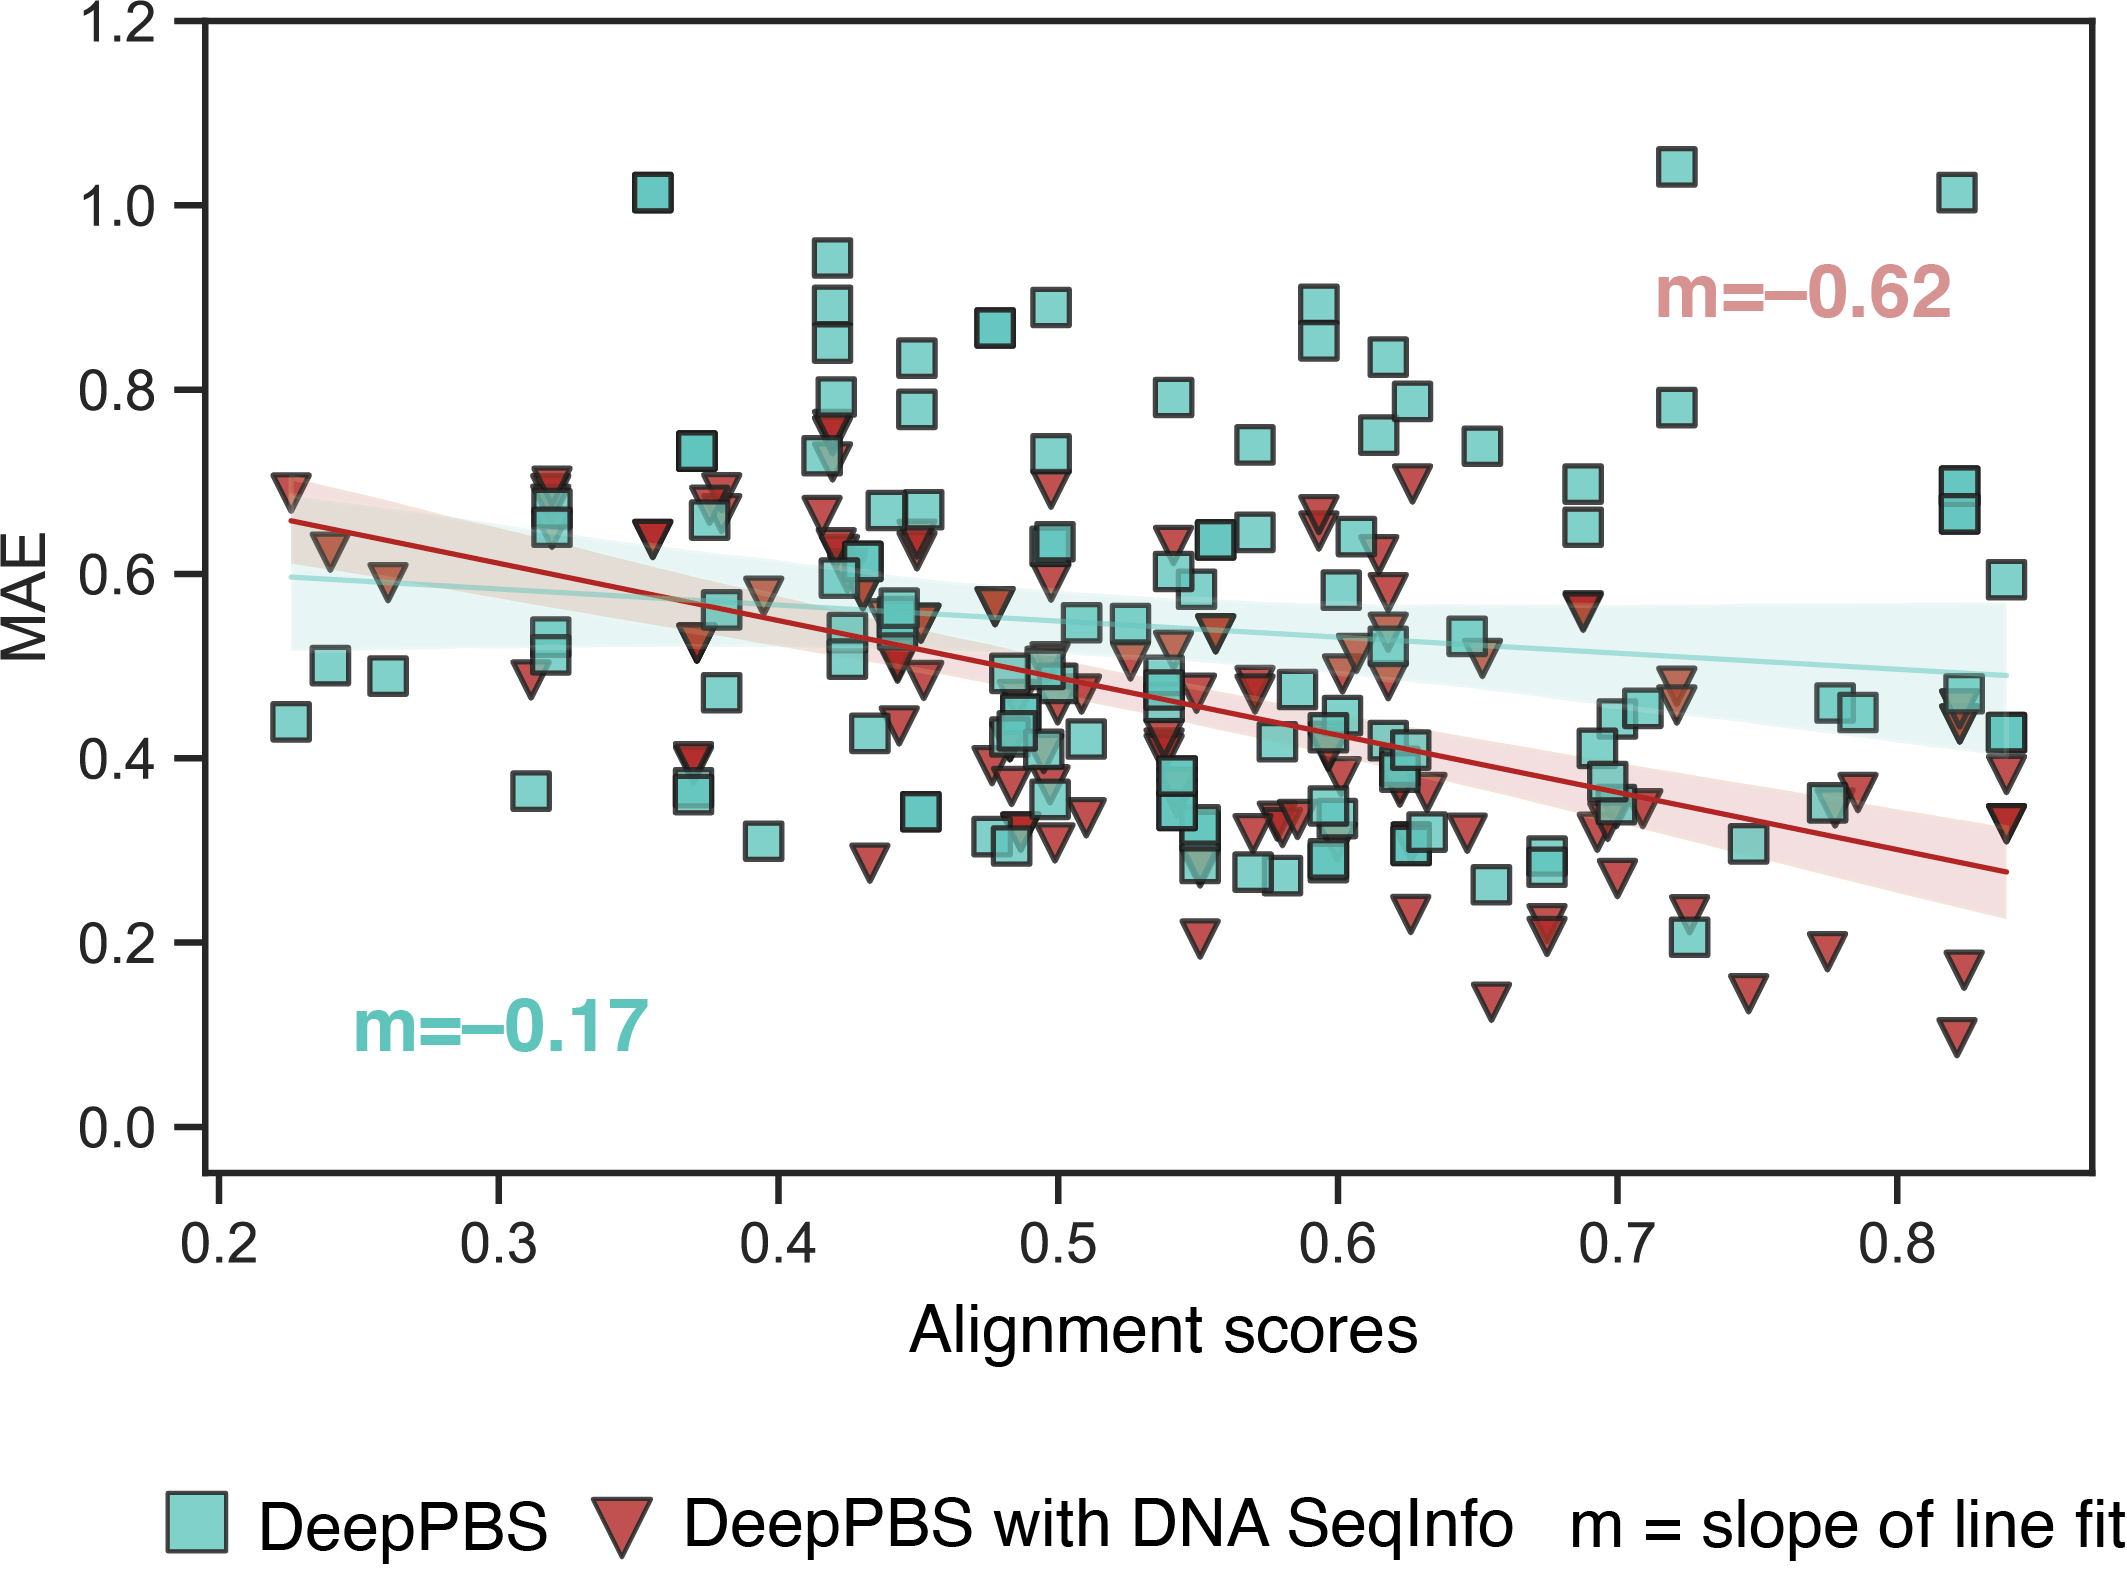
\includegraphics[width=\linewidth]{./pdnafigs/figS11.png}
 % archetecture.png: 1149x508 px, 72dpi, 40.53x17.92 cm, bb=0 0 1149 508
    \caption[Examples of continuous time prediction of ESC differentiation.]{\textbf{Examples of continuous time prediction of ESC differentiation.} Reconstruction (up to $t=6.8$) and future prediction (for $t>6.8$) for 4 example genes by a  latent ODE \citep{chen2018neural} trained on ESC data \citep{Klein2015} for 1000000 iterations, showing a good fit for the initial timepoints, but underfitting for the later timepoints.}
  \label{fig:pdnaS11}
\end{figure}
\end{center}

\begin{center}
\begin{figure}[H]
  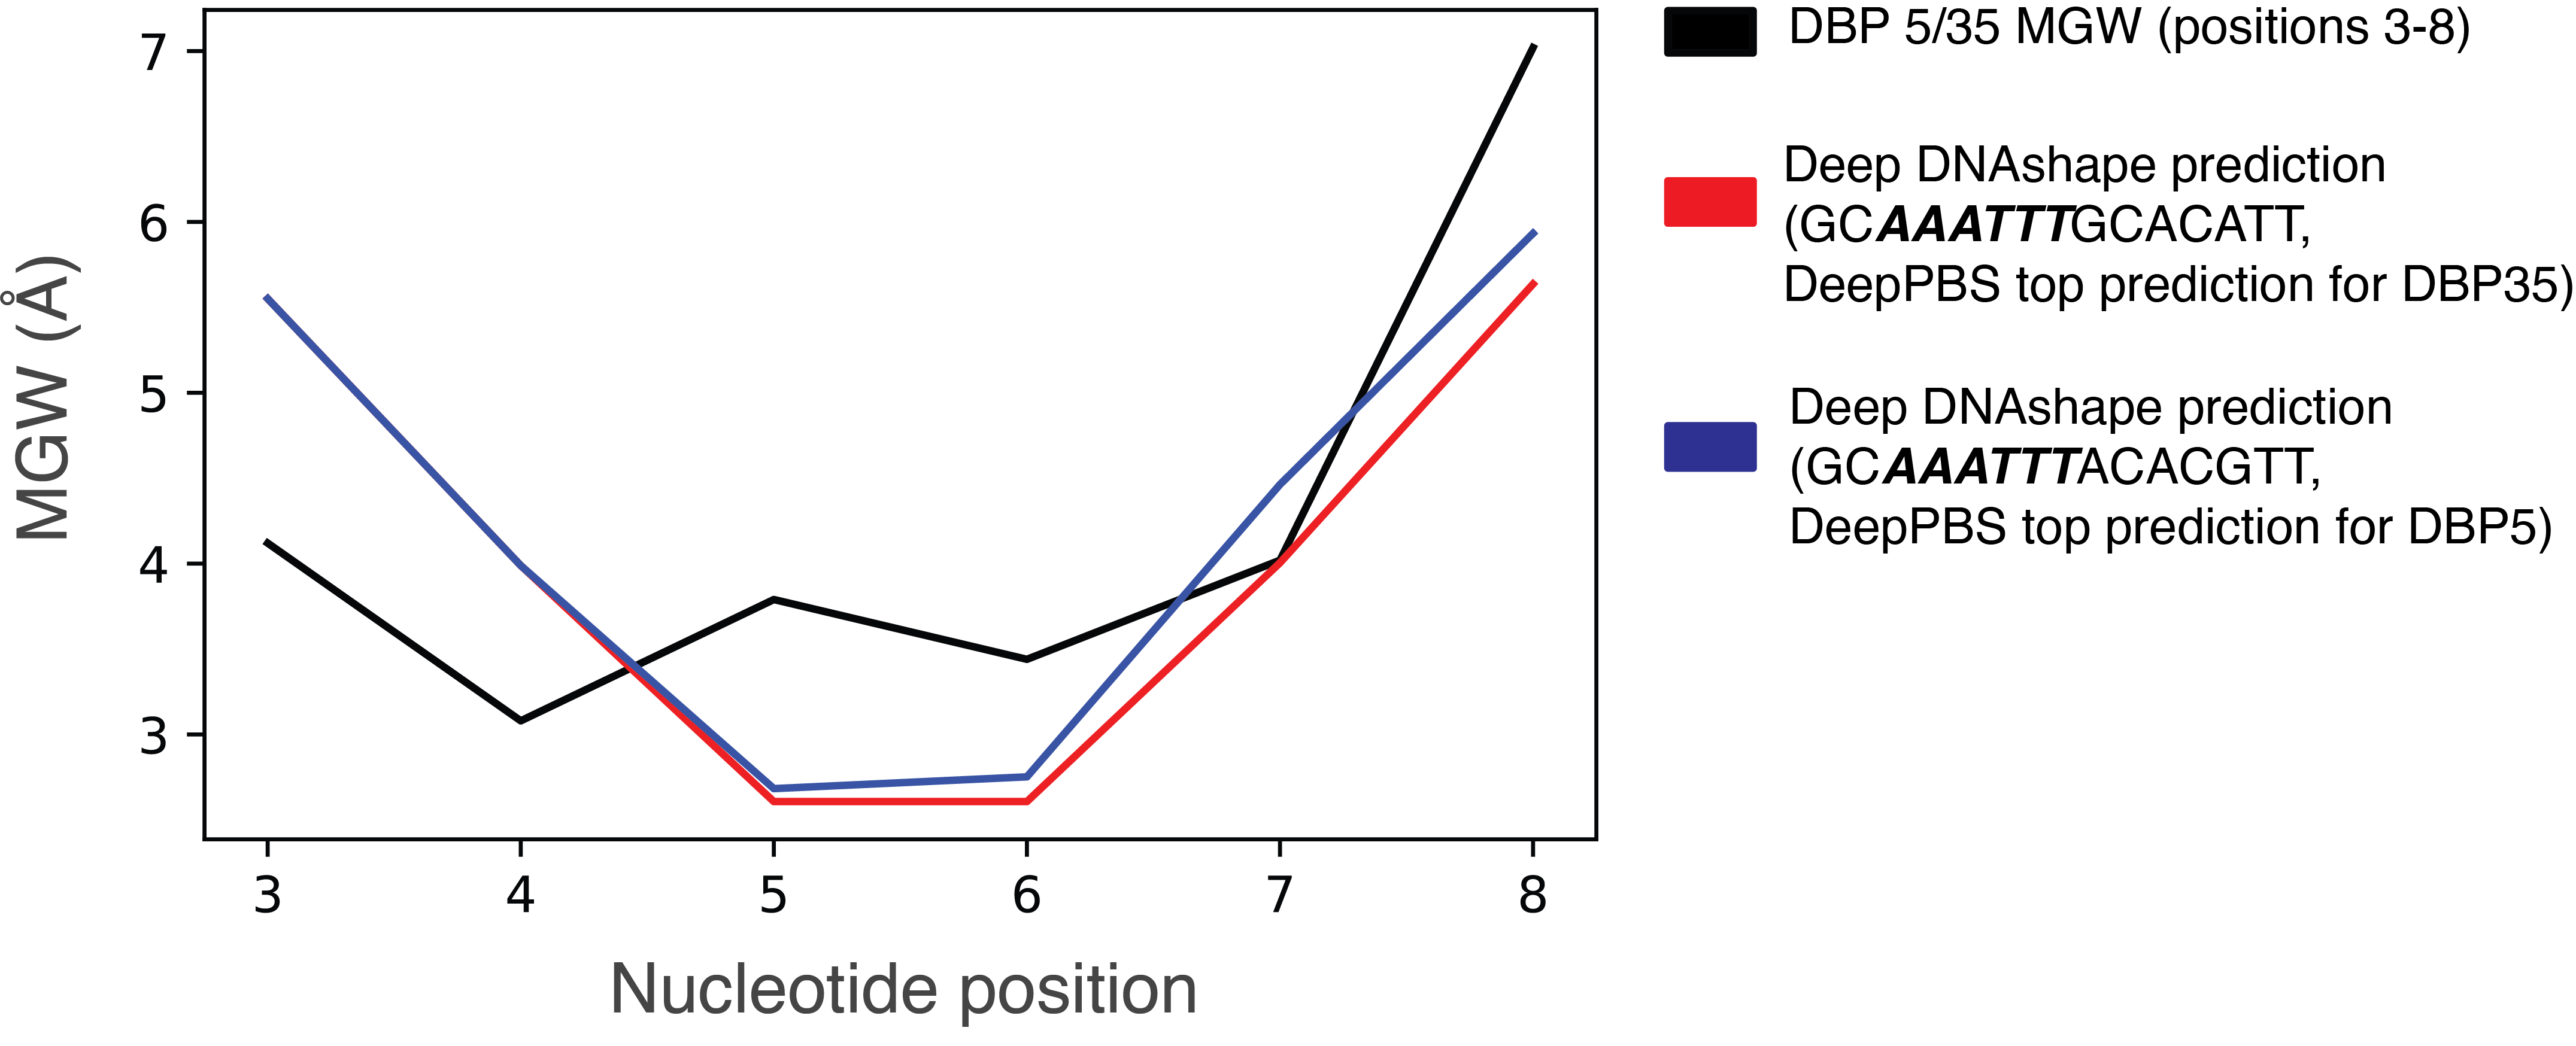
\includegraphics[width=\linewidth]{./pdnafigs/figS12.png}
 % archetecture.png: 1149x508 px, 72dpi, 40.53x17.92 cm, bb=0 0 1149 508
    \caption[Examples of continuous time prediction of ESC differentiation.]{\textbf{Examples of continuous time prediction of ESC differentiation.} Reconstruction (up to $t=6.8$) and future prediction (for $t>6.8$) for 4 example genes by a  latent ODE \citep{chen2018neural} trained on ESC data \citep{Klein2015} for 1000000 iterations, showing a good fit for the initial timepoints, but underfitting for the later timepoints.}
  \label{fig:pdnaS12}
\end{figure}
\end{center}

% Appendices
\phantomsection
\addcontentsline{toc}{chapter}{Appendices}%
\markboth{Appendices}{Appendices}%
\chapter*{Appendices}
\renewcommand\thesection{\Alph{section}}
\renewcommand*{\thesubsection}{\Alph{section}.\arabic{subsection}}
\begingroup
\numberwithin{equation}{section}
% Appendix source files
%\section{A Long Proof}
\label{app:long_proof}

\subsection{Part one}
A long proof that nobody is gonna read goes here.

\subsection{Part two}
Part two of the long proof that nobody is gonna read goes here.

\Blindtext[1]


%SetFonts


%\date{}							% Activate to display a given date or no date

\section*{Detailed calculation of the CCRF layer update}
Starting from the mean field variational inference result in eq. \ref{mean_field_VI_result} we have, %\red{(Kr\"{a}henb\"{u}hl, 2012)} we have,
\label{crf_detailed}
\begin{equation}
Q_i (H_i) \simeq \frac{1}{Z} \exp \left ( - \alpha || H_i - B_i ||^2  - \beta \sum_{j \in \mathcal{N}(i)} g_{ij} \int_{-\infty}^{\infty} Q(H_j) ||H_i - H_j ||^2 d H_j\right )
\end{equation}

where $H_i, B_i, H_j \in \mathbb{R}^N$. Evaluating this component-wise and using the definition of the $\ell_2$ norm, we can write the energy $E(H_i)$ as

\begin{equation}
E(H_i) = \alpha \sum_n^N (H_{in} - B_{in})^2 + \beta \sum_{j \in \mathcal{N}(i)} g_{ij} \sum_n^N \int_{-\infty}^{\infty} \cdots \int_{-\infty}^{\infty} Q(H_j) (H_{in} - H_{jn})^2 d H_{j1}\cdots dH_{jN}
\end{equation}.

Focusing on the inner most summation of second term, since each component of $H_i$ and $H_j$ is
independent (by eq. 10 of \citet{gao2019conditional}), we can write $Q(H_j) = \Pi_{k=1}^N Q_{jk}(H_{jk})$ and assume that each $Q_{jk}$ is individually normalized. The summation then becomes

\begin{multline}
 \sum_n^N \int_{-\infty}^{\infty}  Q(H_j) (H_{in} - H_{jn})^2 d H_{j1}\cdots dH_{jN} \\
= \sum_n^N \int_{-\infty}^{\infty} (H_{in} - H_{jn})^2  \Pi_{k=1}^N Q_{jk}(H_{jk}) d H_{jk} \\
= \sum_n^N \int_{-\infty}^{\infty} (H_{in} - H_{jn})^2  Q_{jn}(H_{jn}) d H_{jn}\int_{-\infty}^{\infty}  \Pi_{k\neq n}^N Q_{jk}(H_{jk}) d H_{jk} \\
\end{multline} 

where the last step follows because all the $Q_{jk}$'s integrate to 1. Therefore, we have that the energy is given by

\begin{equation}
E(H_i) = \sum_n^N \left [ \alpha (H_{in} - B_{in})^2 + \beta \sum_{j \in \mathcal{N}(i)} g_{ij}  \int_{-\infty}^{\infty} (H_{in} - H_{jn})^2  Q_{jn}(H_{jn}) d H_{jn} \right ]
\end{equation}

Taking the derivative of $E(H_i)$ with respect to the $k$ component of $H_i$ we have

\begin{multline}
\frac{\partial E(H_i)} {\partial H_{ik}} = 2\alpha (H_{ik} - B_{ik}) + \beta \sum_{j \in \mathcal{N}(i)} g_{ij} \int_{-\infty}^{\infty} 2 (H_{ik} - H_{jk})  Q_{jn}(H_{jk}) d H_{jk} \\
= 2\alpha (H_{ik} - B_{ik}) + 2\beta \sum_{j \in \mathcal{N}(i)} g_{ij}  (H_{ik} - \int_{-\infty}^{\infty} H_{jk} Q_{jk}(H_{jk})d H_{jk})
\end{multline}

setting this equal to zero and solving for $H_i$ we have

\begin{equation}
H_{ik}^* = \frac{\alpha B_{ik} + \beta  \sum\limits_{j \in \mathcal{N}(i)} g_{ij} \mathbb{E}_{ H_{jk} \sim Q_{jk} } [H_{jk}]} {\alpha +  \beta  \sum \limits_{j \in \mathcal{N}(i)} g_{ij} }
\end{equation}
%%%%%%% Raktim's section %%%%%%%%%%%%%%%%
\section*{Proposed Algorithm}
Given initial states $B_i$ of the nodes, $H_i^0 = B_i$ maximizes $Q_i^0 = \frac{1}{Z_i^0}exp(-c||H_i^0 - B_i||^2)$. Now, we can use the above update equation and approximately     compute (at $t$ th iteration) $H_i^{t+1}$ (maximising $Q_i^{t+1})$ using $H_i^t$ and so forth until convergence (i.e. upto some iteration K, after which $Q_i^t$ and $Q_i^{t+1}$ are not very different and hence, so are $H_i^{T}$ and $H_i^{T+1}$).
\\
Update for iteration k:
\begin{equation}
 H_{i}^{t+1} = \frac{\alpha B_{i} + \beta  \sum\limits_{j \in \mathcal{N}(i)} (g_{ij} H_j^t)} {\alpha +  \beta  \sum \limits_{j \in \mathcal{N}(i)} g_{ij} }
\end{equation}

We can get the aggregated values $(\sum \limits_{j \in \mathcal{N}(i)} (g_{ij} H_j^t),\sum \limits_{j \in \mathcal{N}(i)} g_{ij})$ for $i$th node in a message passing step using $E, B_i$ and $H_i^t$ $\forall i$.
%\begin{pmialgorithm}[0.9\textwidth]{H}{ Mean Field CCRF Layer}\vskip-2ex
%	\label{algo:tk-means}
%	\begin{algorithmic}[1]
%		\REQUIRE  $B_i$  $\forall i$, $E$ (adjacency information)
%		\STATE Initialize $H_i^0 = B_i$ $\forall i$\COMMENT{$H_i^0$ maximizes $Q_i^0 = \frac{1}{Z_i^0}exp(-c||H_i^0 - B_i||^2)$}
%		\FOR[$T$ signifies convergence]{$t=0,1,2,...,T-1$} 
%        \STATE compute $(\sum \limits_{j \in \mathcal{N}(i)} (g_{ij} H_j^t),\sum \limits_{j \in \mathcal{N}(i)} g_{ij})$ \COMMENT{message passing}
%        \STATE $H_i^{t'} = \alpha B_{i} + \beta  \sum\limits_{j \in \mathcal{N}(i)} (g_{ij} H_j^t)$ 
%        \STATE $H_i^{t+1} = H_i^{t'} / (\alpha +  \beta  \sum \limits_{j \in \mathcal{N}(i)} g_{ij} )$ 
%		\ENDFOR 
%		\STATE $H_i^* = H_i^T$
%		\RETURN $H_i^*$
%	\end{algorithmic}
%\end{pmialgorithm}
%Continued in next page ...
%\newpage
\section*{$Q_i^{(t)}$ and $H_i^{(t)}$ calculation for $t=1,2$}
\begin{align*}
\bE_{H_{jk}^{(0)}}[(H_{ik}^{(1)} - H_{jk}^{(0)})^2] &= \int_{x} exp[-\alpha(x - B_{jk})^2 ](H_{ik}^{(1)}-x)^2dx\\
 &=\int_{t} exp[-\alpha(t - (B_{jk} - H_{ik}^{(1)}))^2)t^2dt\\
 &=Var(T) + \bE[T]^2  \hspace{10pt}\text{($T = X - H_{ik}^{(1)}$)}\\
 &= \bE[T]^2 + const.\\
 &= (H_{ik}^{(1)} - B_{jk})^2\\
 \implies Q_i^{(1)} &= \frac{1}{Z_{i}^{(1)}}exp(-E(H_i^{(1)}))\\
 \implies E(H_i^{(1)}) &= \sum_{k=1}^{N}[\alpha(H_{ik}^{(1)} - B_{ik})^2 + \beta\sum_{j\in\cN(i)}g_{ij}(H_{ik}^{(1)} - B_{jk})^2]\\
 \text{Taking partial derivative and setting to 0:}\\
 H_{ik}^{(1)} &= \frac{\alpha B_{ik} +  \beta\sum_{j\in\cN(i)}g_{ij}B_{jk}}{\alpha + \beta\sum_{j\in\cN(i)}g_{ij}}\\
 ----- & ------\\
 \end{align*}
\begin{align*}
 \bE_{H_{jk}^{(1)}}[(H_{ik}^{(2)} - H_{jk}^{(1)})^2] &= \int_{x} exp[-\alpha(x - B_{jk})^2 - \beta\sum_{p\in\cN(j)}g_{jp}(x - B_{pk})^2](H_{ik}^{(2)}-x)^2dx\\
        &=\int_{t} exp[-\alpha(t - (B_{jk} - H_{ik}^{(2)}))^2 - \beta\sum_{p\in\cN(j)}g_{ip}(t  - (B_{pk} -H_{ik}^{(2)}))^2]t^2dt\\
 &=Var(T) + \bE[T]^2  \hspace{10pt}\text{($T = X - H_{ik}^{(2)}$)}\\
 &= \bE[T]^2 + const.\\
\end{align*}
\newpage
\begin{align*}
\bE[T] &= argmin_{t} (\alpha(t - (B_{jk} - H_{ik}^{(2)}))^2 + \beta\sum_{p\in\cN(j)}g_{jp}(t  - (B_{pk} -H_{ik}^{(2)}))^2)\\
\implies \bE[T] &= \frac{\alpha(B_{jk} - H_{ik}^{(2)}) + \beta\sum_{p\in\cN(j)}g_{jp}(B_{pk} -H_{ik}^{(2)})}{\alpha + \beta\sum_{p\in\cN(j)}g_{jp}} \\
\implies \bE[(H_{ik}^{(2)} - H_{jk}^{(1)})^2] &= \Big{[}\frac{\alpha(B_{jk} - H_{ik}^{(2)}) + \beta\sum_{p\in\cN(j)}g_{jp}(B_{pk} -H_{ik}^{(2)})}{\alpha + \beta\sum_{p\in\cN(j)}g_{jp}}\Big{]}^2\\
&=\Big{[}\frac{\alpha(H_{ik}^{(2)} - B_{jk}) + \beta\sum_{p\in\cN(j)}g_{jp}(H_{ik}^{(2)} - B_{pk})}{\alpha + \beta\sum_{p\in\cN(j)}g_{jp}}\Big{]}^2\\
&= \Big{[}\frac{H_{ik}^{(2)}(\alpha + \beta\sum_{p\in\cN(j)}g_{jp})}{\alpha + \beta\sum_{p\in\cN(j)}g_{jp}} - \frac{\alpha B_{jk} +  \beta\sum_{p\in\cN(j)}g_{jp}B_{pk}}{\alpha + \beta\sum_{p\in\cN(j)}g_{jp}}\Big{]}^2\\
&= \Big{[}H_{ik}^{(2)} - \frac{\alpha B_{jk} +  \beta\sum_{p\in\cN(j)}g_{jp}B_{pk}}{\alpha + \beta\sum_{p   \in\cN(j)}g_{jp}}\Big{]}^2\\
&=\Big{[}H_{ik}^{(2)} - H_{jk}^{(1)}\Big{]}^2\\
 &-----------\\
\end{align*} 
\begin{align*}
 Q_i^{(2)} &= \frac{1}{Z_{i}^{(2)}}exp(-E(H_i^{(2)})) \\
 \implies E(H_i^{(2)}) &= \sum_{k=1}^{N}[\alpha(H_{ik}^{(2)} - B_{ik})^2 + \beta\sum_{j\in\cN(i)}g_{ij}(H_{ik}^{(2)} - H_{jk}^{(1)})^2]\\
 \text{Taking partial derivative and setting to 0:}\\
 H_{ik}^{(2)} &= \frac{\alpha B_{ik} +  \beta\sum_{j\in\cN(i)}g_{ij}H_{jk}^{(1)}}{\alpha + \beta\sum_{j\in\cN(i)}g_{ij}}\\
\end{align*}
Similarly we can show the updates of eq.(7) holds true for t=3,4,...
\begin{center}
 ---------------------------------------
\end{center}


\endgroup

% In case your dissertation has multiple volumes.
% \addvolumecontents{thesis_part2}
% \addvolumecontents{thesis_part3}
% \addvolumecontents[lof]{thesis_part2}

\end{document}
